\documentclass[twoside]{book}

% Packages required by doxygen
\usepackage{fixltx2e}
\usepackage{calc}
\usepackage{doxygen}
\usepackage[export]{adjustbox} % also loads graphicx
\usepackage{graphicx}
\usepackage[utf8]{inputenc}
\usepackage{makeidx}
\usepackage{multicol}
\usepackage{multirow}
\PassOptionsToPackage{warn}{textcomp}
\usepackage{textcomp}
\usepackage[nointegrals]{wasysym}
\usepackage[table]{xcolor}

% Font selection
\usepackage[T1]{fontenc}
\usepackage[scaled=.90]{helvet}
\usepackage{courier}
\usepackage{amssymb}
\usepackage{sectsty}
\renewcommand{\familydefault}{\sfdefault}
\allsectionsfont{%
  \fontseries{bc}\selectfont%
  \color{darkgray}%
}
\renewcommand{\DoxyLabelFont}{%
  \fontseries{bc}\selectfont%
  \color{darkgray}%
}
\newcommand{\+}{\discretionary{\mbox{\scriptsize$\hookleftarrow$}}{}{}}

% Page & text layout
\usepackage{geometry}
\geometry{%
  a4paper,%
  top=2.5cm,%
  bottom=2.5cm,%
  left=2.5cm,%
  right=2.5cm%
}
\tolerance=750
\hfuzz=15pt
\hbadness=750
\setlength{\emergencystretch}{15pt}
\setlength{\parindent}{0cm}
\setlength{\parskip}{3ex plus 2ex minus 2ex}
\makeatletter
\renewcommand{\paragraph}{%
  \@startsection{paragraph}{4}{0ex}{-1.0ex}{1.0ex}{%
    \normalfont\normalsize\bfseries\SS@parafont%
  }%
}
\renewcommand{\subparagraph}{%
  \@startsection{subparagraph}{5}{0ex}{-1.0ex}{1.0ex}{%
    \normalfont\normalsize\bfseries\SS@subparafont%
  }%
}
\makeatother

% Headers & footers
\usepackage{fancyhdr}
\pagestyle{fancyplain}
\fancyhead[LE]{\fancyplain{}{\bfseries\thepage}}
\fancyhead[CE]{\fancyplain{}{}}
\fancyhead[RE]{\fancyplain{}{\bfseries\leftmark}}
\fancyhead[LO]{\fancyplain{}{\bfseries\rightmark}}
\fancyhead[CO]{\fancyplain{}{}}
\fancyhead[RO]{\fancyplain{}{\bfseries\thepage}}
\fancyfoot[LE]{\fancyplain{}{}}
\fancyfoot[CE]{\fancyplain{}{}}
\fancyfoot[RE]{\fancyplain{}{\bfseries\scriptsize Generated by Doxygen }}
\fancyfoot[LO]{\fancyplain{}{\bfseries\scriptsize Generated by Doxygen }}
\fancyfoot[CO]{\fancyplain{}{}}
\fancyfoot[RO]{\fancyplain{}{}}
\renewcommand{\footrulewidth}{0.4pt}
\renewcommand{\chaptermark}[1]{%
  \markboth{#1}{}%
}
\renewcommand{\sectionmark}[1]{%
  \markright{\thesection\ #1}%
}

% Indices & bibliography
\usepackage{natbib}
\usepackage[titles]{tocloft}
\setcounter{tocdepth}{3}
\setcounter{secnumdepth}{5}
\makeindex

% Custom commands
\newcommand{\clearemptydoublepage}{%
  \newpage{\pagestyle{empty}\cleardoublepage}%
}

\usepackage{caption}
\captionsetup{labelsep=space,justification=centering,font={bf},singlelinecheck=off,skip=4pt,position=top}

%===== C O N T E N T S =====

\begin{document}

% Titlepage & ToC
\pagenumbering{alph}
\begin{titlepage}
\vspace*{7cm}
\begin{center}%
{\Large Vex Team A \\[1ex]\large 1.\+0.\+2 }\\
\vspace*{1cm}
{\large Generated by Doxygen 1.8.13}\\
\end{center}
\end{titlepage}
\clearemptydoublepage
\pagenumbering{roman}
\tableofcontents
\clearemptydoublepage
\pagenumbering{arabic}

%--- Begin generated contents ---
\chapter{In\+The\+ZoneA}
\label{md__r_e_a_d_m_e}
\input{md__r_e_a_d_m_e}
\chapter{Namespace Index}
\subsection{Namespace List}
Here is a list of all namespaces with brief descriptions\+:\begin{DoxyCompactList}
\item\contentsline{section}{\textbf{ test\+Math} }{\pageref{namespacetest_math}}{}
\end{DoxyCompactList}

\chapter{Data Structure Index}
\section{Data Structures}
Here are the data structures with brief descriptions\+:\begin{DoxyCompactList}
\item\contentsline{section}{\hyperlink{structlcd__buttons}{lcd\+\_\+buttons} \\*Repreents the state of the lcd buttons }{\pageref{structlcd__buttons}}{}
\item\contentsline{section}{\hyperlink{structmenu}{menu} }{\pageref{structmenu}}{}
\item\contentsline{section}{\hyperlink{structmenu__result}{menu\+\_\+result} }{\pageref{structmenu__result}}{}
\item\contentsline{section}{\hyperlink{structpolar__cord}{polar\+\_\+cord} \\*A struct that contains polar cordinates }{\pageref{structpolar__cord}}{}
\end{DoxyCompactList}

\chapter{File Index}
\section{File List}
Here is a list of all files with brief descriptions\+:\begin{DoxyCompactList}
\item\contentsline{section}{\textbf{ test\+Math.\+py} }{\pageref{test_math_8py}}{}
\item\contentsline{section}{include/\textbf{ auto.\+h} \\*Autonomous declarations and macros }{\pageref{auto_8h}}{}
\item\contentsline{section}{include/\textbf{ battery.\+h} \\*Battery management related functions }{\pageref{battery_8h}}{}
\item\contentsline{section}{include/\textbf{ claw.\+h} \\*Code for controlling the claw that grabs the cones }{\pageref{claw_8h}}{}
\item\contentsline{section}{include/\textbf{ controller.\+h} \\*Controller definitions, macros and functions to assist with usig the vex controllers }{\pageref{controller_8h}}{}
\item\contentsline{section}{include/\textbf{ drive.\+h} \\*Drive base definitions and enumerations }{\pageref{drive_8h}}{}
\item\contentsline{section}{include/\textbf{ encoders.\+h} \\*Wrapper around encoder functions }{\pageref{encoders_8h}}{}
\item\contentsline{section}{include/\textbf{ gyro.\+h} }{\pageref{gyro_8h}}{}
\item\contentsline{section}{include/\textbf{ lcd.\+h} \\*L\+CD wrapper functions and macros }{\pageref{lcd_8h}}{}
\item\contentsline{section}{include/\textbf{ lifter.\+h} \\*Declarations and macros for controlling and manipulating the lifter }{\pageref{lifter_8h}}{}
\item\contentsline{section}{include/\textbf{ localization.\+h} \\*Declarations and macros for determining the location of the robot. [W\+IP] }{\pageref{localization_8h}}{}
\item\contentsline{section}{include/\textbf{ log.\+h} \\*Contains logging functions }{\pageref{log_8h}}{}
\item\contentsline{section}{include/\textbf{ main.\+h} \\*Header file for global functions }{\pageref{main_8h}}{}
\item\contentsline{section}{include/\textbf{ matrix.\+h} \\*Various Matrix operations.

None of the matrix operations below change the input matrices if an input is required. They all return a new matrix with the new changes. Because memory issues are so prevelant, be sure to use the  function to reclaim some of that memory }{\pageref{matrix_8h}}{}
\item\contentsline{section}{include/\textbf{ menu.\+h} \\*Contains menu functionality and abstraction }{\pageref{menu_8h}}{}
\item\contentsline{section}{include/\textbf{ mobile\+\_\+goal\+\_\+intake.\+h} }{\pageref{mobile__goal__intake_8h}}{}
\item\contentsline{section}{include/\textbf{ motor\+\_\+ports.\+h} \\*The motor port definitions

Macros for the different motors ports }{\pageref{motor__ports_8h}}{}
\item\contentsline{section}{include/\textbf{ partner.\+h} }{\pageref{partner_8h}}{}
\item\contentsline{section}{include/\textbf{ potentiometer.\+h} }{\pageref{potentiometer_8h}}{}
\item\contentsline{section}{include/\textbf{ sensor\+\_\+ports.\+h} }{\pageref{sensor__ports_8h}}{}
\item\contentsline{section}{include/\textbf{ slew.\+h} \\*Contains the slew rate controller wrapper for the motors }{\pageref{slew_8h}}{}
\item\contentsline{section}{include/\textbf{ toggle.\+h} }{\pageref{toggle_8h}}{}
\item\contentsline{section}{include/\textbf{ vlib.\+h} \\*Contains misc helpful functions }{\pageref{vlib_8h}}{}
\item\contentsline{section}{include/\textbf{ vmath.\+h} \\*Vex Specific Math Functions, includes\+: Cartesian to polar cordinates }{\pageref{vmath_8h}}{}
\item\contentsline{section}{src/\textbf{ auto.\+c} \\*File for autonomous code }{\pageref{auto_8c}}{}
\item\contentsline{section}{src/\textbf{ battery.\+c} }{\pageref{battery_8c}}{}
\item\contentsline{section}{src/\textbf{ claw.\+c} }{\pageref{claw_8c}}{}
\item\contentsline{section}{src/\textbf{ controller.\+c} }{\pageref{controller_8c}}{}
\item\contentsline{section}{src/\textbf{ drive.\+c} }{\pageref{drive_8c}}{}
\item\contentsline{section}{src/\textbf{ encoders.\+c} }{\pageref{encoders_8c}}{}
\item\contentsline{section}{src/\textbf{ gyro.\+c} }{\pageref{gyro_8c}}{}
\item\contentsline{section}{src/\textbf{ init.\+c} \\*File for initialization code }{\pageref{init_8c}}{}
\item\contentsline{section}{src/\textbf{ lcd.\+c} }{\pageref{lcd_8c}}{}
\item\contentsline{section}{src/\textbf{ lifter.\+c} }{\pageref{lifter_8c}}{}
\item\contentsline{section}{src/\textbf{ localization.\+c} }{\pageref{localization_8c}}{}
\item\contentsline{section}{src/\textbf{ log.\+c} }{\pageref{log_8c}}{}
\item\contentsline{section}{src/\textbf{ matrix.\+c} }{\pageref{matrix_8c}}{}
\item\contentsline{section}{src/\textbf{ menu.\+c} }{\pageref{menu_8c}}{}
\item\contentsline{section}{src/\textbf{ mobile\+\_\+goal\+\_\+intake.\+c} }{\pageref{mobile__goal__intake_8c}}{}
\item\contentsline{section}{src/\textbf{ opcontrol.\+c} \\*File for operator control code }{\pageref{opcontrol_8c}}{}
\item\contentsline{section}{src/\textbf{ partner.\+c} }{\pageref{partner_8c}}{}
\item\contentsline{section}{src/\textbf{ slew.\+c} }{\pageref{slew_8c}}{}
\item\contentsline{section}{src/\textbf{ toggle.\+c} }{\pageref{toggle_8c}}{}
\item\contentsline{section}{src/\textbf{ vlib.\+c} }{\pageref{vlib_8c}}{}
\item\contentsline{section}{src/\textbf{ vmath.\+c} }{\pageref{vmath_8c}}{}
\item\contentsline{section}{test\+\_\+code/\textbf{ test\+Math.\+py} }{\pageref{test__code_2test_math_8py}}{}
\end{DoxyCompactList}

\chapter{Namespace Documentation}
\hypertarget{namespacetest_math}{}\section{test\+Math Namespace Reference}
\label{namespacetest_math}\index{test\+Math@{test\+Math}}
\subsection*{Functions}
\begin{DoxyCompactItemize}
\item 
def \hyperlink{namespacetest_math_accae4d78fc0739220d35c06c2c0d5822}{test} (l1, l2)
\end{DoxyCompactItemize}


\subsection{Function Documentation}
\mbox{\Hypertarget{namespacetest_math_accae4d78fc0739220d35c06c2c0d5822}\label{namespacetest_math_accae4d78fc0739220d35c06c2c0d5822}} 
\index{test\+Math@{test\+Math}!test@{test}}
\index{test@{test}!test\+Math@{test\+Math}}
\subsubsection{\texorpdfstring{test()}{test()}}
{\footnotesize\ttfamily def test\+Math.\+test (\begin{DoxyParamCaption}\item[{}]{l1,  }\item[{}]{l2 }\end{DoxyParamCaption})}



Definition at line 3 of file test\+Math.\+py.



References print().


\begin{DoxyCode}
3 \textcolor{keyword}{def }\hyperlink{namespacetest_math_accae4d78fc0739220d35c06c2c0d5822}{test}(l1, l2):
4     \hyperlink{_a_p_i_8h_ae2dd7886efd463e815dadf10eb54777e}{print}(l1, l2)
5     \hyperlink{_a_p_i_8h_ae2dd7886efd463e815dadf10eb54777e}{print}(\textcolor{stringliteral}{"\(\backslash\)n"})
6     theta = l1-l2
7     x = ((l2)/(theta) + .5) - ((l2)/(theta) + .5) * cos(theta)
8     y = ((l2)/(theta) + .5) * sin(theta)
9     \hyperlink{_a_p_i_8h_ae2dd7886efd463e815dadf10eb54777e}{print}(x)
10     \hyperlink{_a_p_i_8h_ae2dd7886efd463e815dadf10eb54777e}{print}(y)
11     \hyperlink{_a_p_i_8h_ae2dd7886efd463e815dadf10eb54777e}{print}(degrees(theta))
12     \hyperlink{_a_p_i_8h_ae2dd7886efd463e815dadf10eb54777e}{print}(\textcolor{stringliteral}{"\(\backslash\)n"})
13     \hyperlink{_a_p_i_8h_ae2dd7886efd463e815dadf10eb54777e}{print}(\textcolor{stringliteral}{"\(\backslash\)n"})
14 
15 \hyperlink{namespacetest_math_accae4d78fc0739220d35c06c2c0d5822}{test}(1.0, .5)
16 \hyperlink{namespacetest_math_accae4d78fc0739220d35c06c2c0d5822}{test}(.5, 1.0)
17 \hyperlink{namespacetest_math_accae4d78fc0739220d35c06c2c0d5822}{test}(2.0, .5)
18 \hyperlink{namespacetest_math_accae4d78fc0739220d35c06c2c0d5822}{test}(.5, 2.0)
19 \hyperlink{namespacetest_math_accae4d78fc0739220d35c06c2c0d5822}{test}(1.0, 3.5)
20 \hyperlink{namespacetest_math_accae4d78fc0739220d35c06c2c0d5822}{test}(3.5, 1.0)
21 \hyperlink{namespacetest_math_accae4d78fc0739220d35c06c2c0d5822}{test}(5, .3) 
22 \hyperlink{namespacetest_math_accae4d78fc0739220d35c06c2c0d5822}{test}(.3, 5)
23 \hyperlink{namespacetest_math_accae4d78fc0739220d35c06c2c0d5822}{test}(1.0, 0)
24 \end{DoxyCode}
Here is the call graph for this function\+:\nopagebreak
\begin{figure}[H]
\begin{center}
\leavevmode
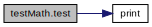
\includegraphics[width=225pt]{namespacetest_math_accae4d78fc0739220d35c06c2c0d5822_cgraph}
\end{center}
\end{figure}

\chapter{Data Structure Documentation}
\section{\+\_\+matrix Struct Reference}
\label{struct__matrix}\index{\+\_\+matrix@{\+\_\+matrix}}


{\ttfamily \#include $<$matrix.\+h$>$}

\subsection*{Data Fields}
\begin{DoxyCompactItemize}
\item 
double $\ast$ \textbf{ data}
\item 
int \textbf{ height}
\item 
int \textbf{ width}
\end{DoxyCompactItemize}


\subsection{Detailed Description}
A struct representing a matrix 

Definition at line \textbf{ 14} of file \textbf{ matrix.\+h}.



\subsection{Field Documentation}
\mbox{\label{struct__matrix_ad3fdadaa9e22623d5830e37663d500be}} 
\index{\+\_\+matrix@{\+\_\+matrix}!data@{data}}
\index{data@{data}!\+\_\+matrix@{\+\_\+matrix}}
\subsubsection{data}
{\footnotesize\ttfamily double$\ast$ \+\_\+matrix\+::data}



Definition at line \textbf{ 17} of file \textbf{ matrix.\+h}.



Referenced by \textbf{ covariance\+Matrix()}, \textbf{ dot\+Diagonal\+Matrix()}, \textbf{ dot\+Product\+Matrix()}, \textbf{ free\+Matrix()}, \textbf{ identity\+Matrix()}, \textbf{ make\+Matrix()}, \textbf{ mean\+Matrix()}, \textbf{ multiply\+Matrix()}, \textbf{ print\+Matrix()}, \textbf{ row\+Swap()}, \textbf{ scale\+Matrix()}, \textbf{ trace\+Matrix()}, and \textbf{ transpose\+Matrix()}.

\mbox{\label{struct__matrix_a8d3b2dbcf98704f11073d646273eb3b0}} 
\index{\+\_\+matrix@{\+\_\+matrix}!height@{height}}
\index{height@{height}!\+\_\+matrix@{\+\_\+matrix}}
\subsubsection{height}
{\footnotesize\ttfamily int \+\_\+matrix\+::height}



Definition at line \textbf{ 15} of file \textbf{ matrix.\+h}.



Referenced by \textbf{ covariance\+Matrix()}, \textbf{ dot\+Diagonal\+Matrix()}, \textbf{ dot\+Product\+Matrix()}, \textbf{ make\+Matrix()}, \textbf{ mean\+Matrix()}, \textbf{ multiply\+Matrix()}, \textbf{ print\+Matrix()}, \textbf{ row\+Swap()}, \textbf{ scale\+Matrix()}, \textbf{ trace\+Matrix()}, and \textbf{ transpose\+Matrix()}.

\mbox{\label{struct__matrix_a30d055d00e1b4afea4568f2aa1cf5c37}} 
\index{\+\_\+matrix@{\+\_\+matrix}!width@{width}}
\index{width@{width}!\+\_\+matrix@{\+\_\+matrix}}
\subsubsection{width}
{\footnotesize\ttfamily int \+\_\+matrix\+::width}



Definition at line \textbf{ 16} of file \textbf{ matrix.\+h}.



Referenced by \textbf{ covariance\+Matrix()}, \textbf{ dot\+Diagonal\+Matrix()}, \textbf{ dot\+Product\+Matrix()}, \textbf{ make\+Matrix()}, \textbf{ mean\+Matrix()}, \textbf{ multiply\+Matrix()}, \textbf{ print\+Matrix()}, \textbf{ row\+Swap()}, \textbf{ scale\+Matrix()}, \textbf{ trace\+Matrix()}, and \textbf{ transpose\+Matrix()}.



The documentation for this struct was generated from the following file\+:\begin{DoxyCompactItemize}
\item 
include/\textbf{ matrix.\+h}\end{DoxyCompactItemize}

\subsection{accelerometer\+\_\+odometry Struct Reference}
\label{structaccelerometer__odometry}\index{accelerometer\+\_\+odometry@{accelerometer\+\_\+odometry}}
\subsubsection*{Data Fields}
\begin{DoxyCompactItemize}
\item 
double \textbf{ x}
\item 
double \textbf{ y}
\end{DoxyCompactItemize}


\subsubsection{Detailed Description}


Definition at line \textbf{ 18} of file \textbf{ localization.\+c}.



\subsubsection{Field Documentation}
\mbox{\label{structaccelerometer__odometry_a83af671d99413a7c480678d5abb9c64a}} 
\index{accelerometer\+\_\+odometry@{accelerometer\+\_\+odometry}!x@{x}}
\index{x@{x}!accelerometer\+\_\+odometry@{accelerometer\+\_\+odometry}}
\paragraph{x}
{\footnotesize\ttfamily double accelerometer\+\_\+odometry\+::x}



Definition at line \textbf{ 19} of file \textbf{ localization.\+c}.

\mbox{\label{structaccelerometer__odometry_a4d812f516efdd477ae9f74fca2a07a2b}} 
\index{accelerometer\+\_\+odometry@{accelerometer\+\_\+odometry}!y@{y}}
\index{y@{y}!accelerometer\+\_\+odometry@{accelerometer\+\_\+odometry}}
\paragraph{y}
{\footnotesize\ttfamily double accelerometer\+\_\+odometry\+::y}



Definition at line \textbf{ 20} of file \textbf{ localization.\+c}.



The documentation for this struct was generated from the following file\+:\begin{DoxyCompactItemize}
\item 
src/\textbf{ localization.\+c}\end{DoxyCompactItemize}

\hypertarget{structcord}{}\section{cord Struct Reference}
\label{structcord}\index{cord@{cord}}


A struct that contains cartesian coordinates.  




{\ttfamily \#include $<$vmath.\+h$>$}

\subsection*{Data Fields}
\begin{DoxyCompactItemize}
\item 
float \hyperlink{structcord_a2eef9b681474b679cf87b0c20eced2cd}{x}
\item 
float \hyperlink{structcord_a4e7d289c55cfe511532e53a81dc19215}{y}
\end{DoxyCompactItemize}


\subsection{Detailed Description}
A struct that contains cartesian coordinates. 

\begin{DoxyDate}{Date}
9/9/2017 
\end{DoxyDate}
\begin{DoxyAuthor}{Author}
Chris Jerrett 
\end{DoxyAuthor}


Definition at line 32 of file vmath.\+h.



\subsection{Field Documentation}
\mbox{\Hypertarget{structcord_a2eef9b681474b679cf87b0c20eced2cd}\label{structcord_a2eef9b681474b679cf87b0c20eced2cd}} 
\index{cord@{cord}!x@{x}}
\index{x@{x}!cord@{cord}}
\subsubsection{\texorpdfstring{x}{x}}
{\footnotesize\ttfamily float cord\+::x}

the x coordinate 

Definition at line 34 of file vmath.\+h.



Referenced by get\+\_\+joystick\+\_\+cord(), and update\+\_\+drive\+\_\+motors().

\mbox{\Hypertarget{structcord_a4e7d289c55cfe511532e53a81dc19215}\label{structcord_a4e7d289c55cfe511532e53a81dc19215}} 
\index{cord@{cord}!y@{y}}
\index{y@{y}!cord@{cord}}
\subsubsection{\texorpdfstring{y}{y}}
{\footnotesize\ttfamily float cord\+::y}

the y coordinate 

Definition at line 36 of file vmath.\+h.



Referenced by get\+\_\+joystick\+\_\+cord(), and update\+\_\+drive\+\_\+motors().



The documentation for this struct was generated from the following file\+:\begin{DoxyCompactItemize}
\item 
include/\hyperlink{vmath_8h}{vmath.\+h}\end{DoxyCompactItemize}

\section{encoder\+\_\+odemtry Struct Reference}
\label{structencoder__odemtry}\index{encoder\+\_\+odemtry@{encoder\+\_\+odemtry}}
\subsection*{Data Fields}
\begin{DoxyCompactItemize}
\item 
double \textbf{ theta}
\item 
double \textbf{ x}
\item 
double \textbf{ y}
\end{DoxyCompactItemize}


\subsection{Detailed Description}


Definition at line \textbf{ 11} of file \textbf{ localization.\+c}.



\subsection{Field Documentation}
\mbox{\label{structencoder__odemtry_af1a1e2a2a7a2f89138a8c261a3b82898}} 
\index{encoder\+\_\+odemtry@{encoder\+\_\+odemtry}!theta@{theta}}
\index{theta@{theta}!encoder\+\_\+odemtry@{encoder\+\_\+odemtry}}
\subsubsection{theta}
{\footnotesize\ttfamily double encoder\+\_\+odemtry\+::theta}



Definition at line \textbf{ 14} of file \textbf{ localization.\+c}.



Referenced by \textbf{ integrate\+\_\+gyro\+\_\+w()}.

\mbox{\label{structencoder__odemtry_a9a803978381f9b89a031d520a627cbcf}} 
\index{encoder\+\_\+odemtry@{encoder\+\_\+odemtry}!x@{x}}
\index{x@{x}!encoder\+\_\+odemtry@{encoder\+\_\+odemtry}}
\subsubsection{x}
{\footnotesize\ttfamily double encoder\+\_\+odemtry\+::x}



Definition at line \textbf{ 12} of file \textbf{ localization.\+c}.

\mbox{\label{structencoder__odemtry_a955cbea800158b8c0cd5f36b253fe6bb}} 
\index{encoder\+\_\+odemtry@{encoder\+\_\+odemtry}!y@{y}}
\index{y@{y}!encoder\+\_\+odemtry@{encoder\+\_\+odemtry}}
\subsubsection{y}
{\footnotesize\ttfamily double encoder\+\_\+odemtry\+::y}



Definition at line \textbf{ 13} of file \textbf{ localization.\+c}.



The documentation for this struct was generated from the following file\+:\begin{DoxyCompactItemize}
\item 
src/\textbf{ localization.\+c}\end{DoxyCompactItemize}

\hypertarget{structlcd__buttons}{}\section{lcd\+\_\+buttons Struct Reference}
\label{structlcd__buttons}\index{lcd\+\_\+buttons@{lcd\+\_\+buttons}}


represents the state of the lcd buttons  




{\ttfamily \#include $<$lcd.\+h$>$}

\subsection*{Data Fields}
\begin{DoxyCompactItemize}
\item 
\hyperlink{lcd_8h_a0bbab92f5605e16a4162b6c5ccc2c29b}{button\+\_\+state} \hyperlink{structlcd__buttons_ae385efb5ec794acf5f11027f46c6c039}{left}
\item 
\hyperlink{lcd_8h_a0bbab92f5605e16a4162b6c5ccc2c29b}{button\+\_\+state} \hyperlink{structlcd__buttons_a293342810ac56f73979b08f144d6e6b9}{middle}
\item 
\hyperlink{lcd_8h_a0bbab92f5605e16a4162b6c5ccc2c29b}{button\+\_\+state} \hyperlink{structlcd__buttons_a2437d744e09ca1bb91ab4ca53ef77198}{right}
\end{DoxyCompactItemize}


\subsection{Detailed Description}
represents the state of the lcd buttons 

\begin{DoxyAuthor}{Author}
Chris Jerrett 
\end{DoxyAuthor}
\begin{DoxyDate}{Date}
9/9/2017 
\end{DoxyDate}


Definition at line 48 of file lcd.\+h.



\subsection{Field Documentation}
\mbox{\Hypertarget{structlcd__buttons_ae385efb5ec794acf5f11027f46c6c039}\label{structlcd__buttons_ae385efb5ec794acf5f11027f46c6c039}} 
\index{lcd\+\_\+buttons@{lcd\+\_\+buttons}!left@{left}}
\index{left@{left}!lcd\+\_\+buttons@{lcd\+\_\+buttons}}
\subsubsection{\texorpdfstring{left}{left}}
{\footnotesize\ttfamily \hyperlink{lcd_8h_a0bbab92f5605e16a4162b6c5ccc2c29b}{button\+\_\+state} lcd\+\_\+buttons\+::left}



Definition at line 49 of file lcd.\+h.



Referenced by lcd\+\_\+get\+\_\+pressed\+\_\+buttons().

\mbox{\Hypertarget{structlcd__buttons_a293342810ac56f73979b08f144d6e6b9}\label{structlcd__buttons_a293342810ac56f73979b08f144d6e6b9}} 
\index{lcd\+\_\+buttons@{lcd\+\_\+buttons}!middle@{middle}}
\index{middle@{middle}!lcd\+\_\+buttons@{lcd\+\_\+buttons}}
\subsubsection{\texorpdfstring{middle}{middle}}
{\footnotesize\ttfamily \hyperlink{lcd_8h_a0bbab92f5605e16a4162b6c5ccc2c29b}{button\+\_\+state} lcd\+\_\+buttons\+::middle}



Definition at line 50 of file lcd.\+h.



Referenced by lcd\+\_\+get\+\_\+pressed\+\_\+buttons().

\mbox{\Hypertarget{structlcd__buttons_a2437d744e09ca1bb91ab4ca53ef77198}\label{structlcd__buttons_a2437d744e09ca1bb91ab4ca53ef77198}} 
\index{lcd\+\_\+buttons@{lcd\+\_\+buttons}!right@{right}}
\index{right@{right}!lcd\+\_\+buttons@{lcd\+\_\+buttons}}
\subsubsection{\texorpdfstring{right}{right}}
{\footnotesize\ttfamily \hyperlink{lcd_8h_a0bbab92f5605e16a4162b6c5ccc2c29b}{button\+\_\+state} lcd\+\_\+buttons\+::right}



Definition at line 51 of file lcd.\+h.



Referenced by lcd\+\_\+get\+\_\+pressed\+\_\+buttons().



The documentation for this struct was generated from the following file\+:\begin{DoxyCompactItemize}
\item 
include/\hyperlink{lcd_8h}{lcd.\+h}\end{DoxyCompactItemize}

\subsection{location Struct Reference}
\label{structlocation}\index{location@{location}}


Vector storing the cartesian cords and an angle.  




{\ttfamily \#include $<$localization.\+h$>$}

\subsubsection*{Data Fields}
\begin{DoxyCompactItemize}
\item 
int \textbf{ theta}
\item 
int \textbf{ x}
\item 
int \textbf{ y}
\end{DoxyCompactItemize}


\subsubsection{Detailed Description}
Vector storing the cartesian cords and an angle. 

Definition at line \textbf{ 24} of file \textbf{ localization.\+h}.



\subsubsection{Field Documentation}
\mbox{\label{structlocation_a4b415222b4dcf34e49dacd22384be9eb}} 
\index{location@{location}!theta@{theta}}
\index{theta@{theta}!location@{location}}
\paragraph{theta}
{\footnotesize\ttfamily int location\+::theta}



Definition at line \textbf{ 27} of file \textbf{ localization.\+h}.

\mbox{\label{structlocation_aacd18b2506c49d221cfc37b2119e3c3c}} 
\index{location@{location}!x@{x}}
\index{x@{x}!location@{location}}
\paragraph{x}
{\footnotesize\ttfamily int location\+::x}



Definition at line \textbf{ 25} of file \textbf{ localization.\+h}.

\mbox{\label{structlocation_ad7197d1981d4ea5d8b36041473cac815}} 
\index{location@{location}!y@{y}}
\index{y@{y}!location@{location}}
\paragraph{y}
{\footnotesize\ttfamily int location\+::y}



Definition at line \textbf{ 26} of file \textbf{ localization.\+h}.



The documentation for this struct was generated from the following file\+:\begin{DoxyCompactItemize}
\item 
include/\textbf{ localization.\+h}\end{DoxyCompactItemize}

\hypertarget{structmenu__t}{}\section{menu\+\_\+t Struct Reference}
\label{structmenu__t}\index{menu\+\_\+t@{menu\+\_\+t}}


Represents a specific instance of a menu. Will cause a memory leak if not deinitialized via denint\+\_\+menu.  




{\ttfamily \#include $<$menu.\+h$>$}

\subsection*{Data Fields}
\begin{DoxyCompactItemize}
\item 
int \hyperlink{structmenu__t_a2acb18066898677ec5e2dc40eec811c5}{current}
\begin{DoxyCompactList}\small\item\em contains the current index of menu. \end{DoxyCompactList}\item 
unsigned int \hyperlink{structmenu__t_a023063461c4a247e574abd6a55faf765}{length}
\begin{DoxyCompactList}\small\item\em contains the length of options char$\ast$$\ast$. \end{DoxyCompactList}\item 
int \hyperlink{structmenu__t_ace9cbaecd7bf311be0ef230da657f406}{max}
\begin{DoxyCompactList}\small\item\em contains the maximum int value of menu. Defaults to minimum int value \end{DoxyCompactList}\item 
float \hyperlink{structmenu__t_a14b11d0a7610484462c8a6e93068a2c1}{max\+\_\+f}
\begin{DoxyCompactList}\small\item\em contains the maximum float value of menu. Defaults to minimum int value \end{DoxyCompactList}\item 
int \hyperlink{structmenu__t_a6891bc6c94f1e995cc62a05b13328de5}{min}
\begin{DoxyCompactList}\small\item\em contains the minimum int value of menu. Defaults to minimum int value \end{DoxyCompactList}\item 
float \hyperlink{structmenu__t_a0a6e4f711992fb69e8a57c2af1ab7a05}{min\+\_\+f}
\begin{DoxyCompactList}\small\item\em contains the minimum float value of menu. Defaults to minimum int value \end{DoxyCompactList}\item 
char $\ast$$\ast$ \hyperlink{structmenu__t_ad695cd88051e34817f0f582d4e43c33a}{options}
\begin{DoxyCompactList}\small\item\em contains the array of string options. \end{DoxyCompactList}\item 
char \hyperlink{structmenu__t_a5e3af2830962c2bbcb0a983f2c040c65}{prompt} \mbox{[}16\mbox{]}
\begin{DoxyCompactList}\small\item\em contains the prompt to display on the first line. Step is how much the int menu will increase of decrease with each press. Defaults to one \end{DoxyCompactList}\item 
int \hyperlink{structmenu__t_adc50450bc59ea66a8d67424adc46e24e}{step}
\begin{DoxyCompactList}\small\item\em contains the step int value of menu. Step is how much the int menu will increase of decrease with each press. Defaults to one \end{DoxyCompactList}\item 
float \hyperlink{structmenu__t_a84cfd9226f6554c63ca9f4b11f94d12d}{step\+\_\+f}
\begin{DoxyCompactList}\small\item\em contains the step float value of menu. Step is how much the int menu will increase of decrease with each press. Defaults to 1.\+0f \end{DoxyCompactList}\item 
enum \hyperlink{menu_8h_a6bbf4baf5018b0d76aab6c2e6bf85e62}{menu\+\_\+type} \hyperlink{structmenu__t_a110244ceb7d2a7cba95cfc5758d61c01}{type}
\begin{DoxyCompactList}\small\item\em contains the type of menu. \end{DoxyCompactList}\end{DoxyCompactItemize}


\subsection{Detailed Description}
Represents a specific instance of a menu. Will cause a memory leak if not deinitialized via denint\+\_\+menu. 

\begin{DoxyAuthor}{Author}
Chris Jerrett 
\end{DoxyAuthor}
\begin{DoxyDate}{Date}
9/8/17 
\end{DoxyDate}
\begin{DoxySeeAlso}{See also}
\hyperlink{menu_8h}{menu.\+h} 

\hyperlink{structmenu__t}{menu\+\_\+t} 

\hyperlink{menu_8c_adcee778eac0edb821427d32949106dc5}{create\+\_\+menu} 

init\+\_\+menu 

\hyperlink{menu_8c_abfadedb104f89f672dd3045499975a71}{display\+\_\+menu} 

\hyperlink{menu_8h_a6bbf4baf5018b0d76aab6c2e6bf85e62}{menu\+\_\+type} 

\hyperlink{menu_8c_a05a36619ac6c9ba4544eddb83ee2a50d}{denint\+\_\+menu} 
\end{DoxySeeAlso}


Definition at line 64 of file menu.\+h.



\subsection{Field Documentation}
\mbox{\Hypertarget{structmenu__t_a2acb18066898677ec5e2dc40eec811c5}\label{structmenu__t_a2acb18066898677ec5e2dc40eec811c5}} 
\index{menu\+\_\+t@{menu\+\_\+t}!current@{current}}
\index{current@{current}!menu\+\_\+t@{menu\+\_\+t}}
\subsubsection{\texorpdfstring{current}{current}}
{\footnotesize\ttfamily int menu\+\_\+t\+::current}



contains the current index of menu. 

\begin{DoxyAuthor}{Author}
Chris Jerrett 
\end{DoxyAuthor}
\begin{DoxyDate}{Date}
9/8/17 
\end{DoxyDate}


Definition at line 138 of file menu.\+h.



Referenced by calculate\+\_\+current\+\_\+display(), and display\+\_\+menu().

\mbox{\Hypertarget{structmenu__t_a023063461c4a247e574abd6a55faf765}\label{structmenu__t_a023063461c4a247e574abd6a55faf765}} 
\index{menu\+\_\+t@{menu\+\_\+t}!length@{length}}
\index{length@{length}!menu\+\_\+t@{menu\+\_\+t}}
\subsubsection{\texorpdfstring{length}{length}}
{\footnotesize\ttfamily unsigned int menu\+\_\+t\+::length}



contains the length of options char$\ast$$\ast$. 

\begin{DoxyAuthor}{Author}
Chris Jerrett 
\end{DoxyAuthor}
\begin{DoxyDate}{Date}
9/8/17 
\end{DoxyDate}


Definition at line 84 of file menu.\+h.



Referenced by calculate\+\_\+current\+\_\+display(), and init\+\_\+menu\+\_\+var().

\mbox{\Hypertarget{structmenu__t_ace9cbaecd7bf311be0ef230da657f406}\label{structmenu__t_ace9cbaecd7bf311be0ef230da657f406}} 
\index{menu\+\_\+t@{menu\+\_\+t}!max@{max}}
\index{max@{max}!menu\+\_\+t@{menu\+\_\+t}}
\subsubsection{\texorpdfstring{max}{max}}
{\footnotesize\ttfamily int menu\+\_\+t\+::max}



contains the maximum int value of menu. Defaults to minimum int value 

\begin{DoxyAuthor}{Author}
Chris Jerrett 
\end{DoxyAuthor}
\begin{DoxyDate}{Date}
9/8/17 
\end{DoxyDate}


Definition at line 100 of file menu.\+h.



Referenced by calculate\+\_\+current\+\_\+display(), create\+\_\+menu(), and init\+\_\+menu\+\_\+int().

\mbox{\Hypertarget{structmenu__t_a14b11d0a7610484462c8a6e93068a2c1}\label{structmenu__t_a14b11d0a7610484462c8a6e93068a2c1}} 
\index{menu\+\_\+t@{menu\+\_\+t}!max\+\_\+f@{max\+\_\+f}}
\index{max\+\_\+f@{max\+\_\+f}!menu\+\_\+t@{menu\+\_\+t}}
\subsubsection{\texorpdfstring{max\+\_\+f}{max\_f}}
{\footnotesize\ttfamily float menu\+\_\+t\+::max\+\_\+f}



contains the maximum float value of menu. Defaults to minimum int value 

\begin{DoxyAuthor}{Author}
Chris Jerrett 
\end{DoxyAuthor}
\begin{DoxyDate}{Date}
9/8/17 
\end{DoxyDate}


Definition at line 124 of file menu.\+h.



Referenced by calculate\+\_\+current\+\_\+display(), create\+\_\+menu(), and init\+\_\+menu\+\_\+float().

\mbox{\Hypertarget{structmenu__t_a6891bc6c94f1e995cc62a05b13328de5}\label{structmenu__t_a6891bc6c94f1e995cc62a05b13328de5}} 
\index{menu\+\_\+t@{menu\+\_\+t}!min@{min}}
\index{min@{min}!menu\+\_\+t@{menu\+\_\+t}}
\subsubsection{\texorpdfstring{min}{min}}
{\footnotesize\ttfamily int menu\+\_\+t\+::min}



contains the minimum int value of menu. Defaults to minimum int value 

\begin{DoxyAuthor}{Author}
Chris Jerrett 
\end{DoxyAuthor}
\begin{DoxyDate}{Date}
9/8/17 
\end{DoxyDate}


Definition at line 92 of file menu.\+h.



Referenced by calculate\+\_\+current\+\_\+display(), create\+\_\+menu(), and init\+\_\+menu\+\_\+int().

\mbox{\Hypertarget{structmenu__t_a0a6e4f711992fb69e8a57c2af1ab7a05}\label{structmenu__t_a0a6e4f711992fb69e8a57c2af1ab7a05}} 
\index{menu\+\_\+t@{menu\+\_\+t}!min\+\_\+f@{min\+\_\+f}}
\index{min\+\_\+f@{min\+\_\+f}!menu\+\_\+t@{menu\+\_\+t}}
\subsubsection{\texorpdfstring{min\+\_\+f}{min\_f}}
{\footnotesize\ttfamily float menu\+\_\+t\+::min\+\_\+f}



contains the minimum float value of menu. Defaults to minimum int value 

\begin{DoxyAuthor}{Author}
Chris Jerrett 
\end{DoxyAuthor}
\begin{DoxyDate}{Date}
9/8/17 
\end{DoxyDate}


Definition at line 116 of file menu.\+h.



Referenced by calculate\+\_\+current\+\_\+display(), create\+\_\+menu(), and init\+\_\+menu\+\_\+float().

\mbox{\Hypertarget{structmenu__t_ad695cd88051e34817f0f582d4e43c33a}\label{structmenu__t_ad695cd88051e34817f0f582d4e43c33a}} 
\index{menu\+\_\+t@{menu\+\_\+t}!options@{options}}
\index{options@{options}!menu\+\_\+t@{menu\+\_\+t}}
\subsubsection{\texorpdfstring{options}{options}}
{\footnotesize\ttfamily char$\ast$$\ast$ menu\+\_\+t\+::options}



contains the array of string options. 

\begin{DoxyAuthor}{Author}
Chris Jerrett 
\end{DoxyAuthor}
\begin{DoxyDate}{Date}
9/8/17 
\end{DoxyDate}


Definition at line 77 of file menu.\+h.



Referenced by calculate\+\_\+current\+\_\+display(), denint\+\_\+menu(), and init\+\_\+menu\+\_\+var().

\mbox{\Hypertarget{structmenu__t_a5e3af2830962c2bbcb0a983f2c040c65}\label{structmenu__t_a5e3af2830962c2bbcb0a983f2c040c65}} 
\index{menu\+\_\+t@{menu\+\_\+t}!prompt@{prompt}}
\index{prompt@{prompt}!menu\+\_\+t@{menu\+\_\+t}}
\subsubsection{\texorpdfstring{prompt}{prompt}}
{\footnotesize\ttfamily char menu\+\_\+t\+::prompt\mbox{[}16\mbox{]}}



contains the prompt to display on the first line. Step is how much the int menu will increase of decrease with each press. Defaults to one 

\begin{DoxyAuthor}{Author}
Chris Jerrett 
\end{DoxyAuthor}
\begin{DoxyDate}{Date}
9/8/17 
\end{DoxyDate}


Definition at line 145 of file menu.\+h.



Referenced by create\+\_\+menu(), denint\+\_\+menu(), and display\+\_\+menu().

\mbox{\Hypertarget{structmenu__t_adc50450bc59ea66a8d67424adc46e24e}\label{structmenu__t_adc50450bc59ea66a8d67424adc46e24e}} 
\index{menu\+\_\+t@{menu\+\_\+t}!step@{step}}
\index{step@{step}!menu\+\_\+t@{menu\+\_\+t}}
\subsubsection{\texorpdfstring{step}{step}}
{\footnotesize\ttfamily int menu\+\_\+t\+::step}



contains the step int value of menu. Step is how much the int menu will increase of decrease with each press. Defaults to one 

\begin{DoxyAuthor}{Author}
Chris Jerrett 
\end{DoxyAuthor}
\begin{DoxyDate}{Date}
9/8/17 
\end{DoxyDate}


Definition at line 108 of file menu.\+h.



Referenced by calculate\+\_\+current\+\_\+display(), create\+\_\+menu(), and init\+\_\+menu\+\_\+int().

\mbox{\Hypertarget{structmenu__t_a84cfd9226f6554c63ca9f4b11f94d12d}\label{structmenu__t_a84cfd9226f6554c63ca9f4b11f94d12d}} 
\index{menu\+\_\+t@{menu\+\_\+t}!step\+\_\+f@{step\+\_\+f}}
\index{step\+\_\+f@{step\+\_\+f}!menu\+\_\+t@{menu\+\_\+t}}
\subsubsection{\texorpdfstring{step\+\_\+f}{step\_f}}
{\footnotesize\ttfamily float menu\+\_\+t\+::step\+\_\+f}



contains the step float value of menu. Step is how much the int menu will increase of decrease with each press. Defaults to 1.\+0f 

\begin{DoxyAuthor}{Author}
Chris Jerrett 
\end{DoxyAuthor}
\begin{DoxyDate}{Date}
9/8/17 
\end{DoxyDate}


Definition at line 132 of file menu.\+h.



Referenced by calculate\+\_\+current\+\_\+display(), create\+\_\+menu(), and init\+\_\+menu\+\_\+float().

\mbox{\Hypertarget{structmenu__t_a110244ceb7d2a7cba95cfc5758d61c01}\label{structmenu__t_a110244ceb7d2a7cba95cfc5758d61c01}} 
\index{menu\+\_\+t@{menu\+\_\+t}!type@{type}}
\index{type@{type}!menu\+\_\+t@{menu\+\_\+t}}
\subsubsection{\texorpdfstring{type}{type}}
{\footnotesize\ttfamily enum \hyperlink{menu_8h_a6bbf4baf5018b0d76aab6c2e6bf85e62}{menu\+\_\+type} menu\+\_\+t\+::type}



contains the type of menu. 

\begin{DoxyAuthor}{Author}
Chris Jerrett 
\end{DoxyAuthor}
\begin{DoxyDate}{Date}
9/8/17 
\end{DoxyDate}


Definition at line 70 of file menu.\+h.



Referenced by calculate\+\_\+current\+\_\+display(), and create\+\_\+menu().



The documentation for this struct was generated from the following file\+:\begin{DoxyCompactItemize}
\item 
include/\hyperlink{menu_8h}{menu.\+h}\end{DoxyCompactItemize}

\subsection{polar\+\_\+cord Struct Reference}
\label{structpolar__cord}\index{polar\+\_\+cord@{polar\+\_\+cord}}


A struct that contains polar coordinates.  




{\ttfamily \#include $<$vmath.\+h$>$}

\subsubsection*{Data Fields}
\begin{DoxyCompactItemize}
\item 
float \textbf{ angle}
\begin{DoxyCompactList}\small\item\em the angle of the vector \end{DoxyCompactList}\item 
float \textbf{ magnitue}
\begin{DoxyCompactList}\small\item\em the magnitude of the vector \end{DoxyCompactList}\end{DoxyCompactItemize}


\subsubsection{Detailed Description}
A struct that contains polar coordinates. 

\begin{DoxyDate}{Date}
9/9/2017 
\end{DoxyDate}
\begin{DoxyAuthor}{Author}
Chris Jerrett 
\end{DoxyAuthor}


Definition at line \textbf{ 24} of file \textbf{ vmath.\+h}.



\subsubsection{Field Documentation}
\mbox{\label{structpolar__cord_a81b3a11d38d76719b02fcd425adaa216}} 
\index{polar\+\_\+cord@{polar\+\_\+cord}!angle@{angle}}
\index{angle@{angle}!polar\+\_\+cord@{polar\+\_\+cord}}
\paragraph{angle}
{\footnotesize\ttfamily float polar\+\_\+cord\+::angle}



the angle of the vector 



Definition at line \textbf{ 26} of file \textbf{ vmath.\+h}.



Referenced by \textbf{ cartesian\+\_\+to\+\_\+polar()}.

\mbox{\label{structpolar__cord_aec2e25fecc82af176f0fcd23f1e02f0c}} 
\index{polar\+\_\+cord@{polar\+\_\+cord}!magnitue@{magnitue}}
\index{magnitue@{magnitue}!polar\+\_\+cord@{polar\+\_\+cord}}
\paragraph{magnitue}
{\footnotesize\ttfamily float polar\+\_\+cord\+::magnitue}



the magnitude of the vector 



Definition at line \textbf{ 28} of file \textbf{ vmath.\+h}.



Referenced by \textbf{ cartesian\+\_\+to\+\_\+polar()}.



The documentation for this struct was generated from the following file\+:\begin{DoxyCompactItemize}
\item 
include/\textbf{ vmath.\+h}\end{DoxyCompactItemize}

\chapter{File Documentation}
\section{include/auto.h File Reference}
\label{auto_8h}\index{include/auto.\+h@{include/auto.\+h}}


Autonomous declarations and macros.  


{\ttfamily \#include \char`\"{}drive.\+h\char`\"{}}\newline
{\ttfamily \#include \char`\"{}sensor\+\_\+ports.\+h\char`\"{}}\newline
{\ttfamily \#include \char`\"{}lifter.\+h\char`\"{}}\newline
{\ttfamily \#include \char`\"{}claw.\+h\char`\"{}}\newline
Include dependency graph for auto.\+h\+:
\nopagebreak
\begin{figure}[H]
\begin{center}
\leavevmode
\includegraphics[width=350pt]{auto_8h__incl}
\end{center}
\end{figure}
This graph shows which files directly or indirectly include this file\+:
\nopagebreak
\begin{figure}[H]
\begin{center}
\leavevmode
\includegraphics[width=158pt]{auto_8h__dep__incl}
\end{center}
\end{figure}
\subsection*{Macros}
\begin{DoxyCompactItemize}
\item 
\#define \textbf{ F\+R\+O\+N\+T\+\_\+\+L\+E\+F\+T\+\_\+\+I\+ME}~0
\begin{DoxyCompactList}\small\item\em Front left motor integrated motor encoder. \end{DoxyCompactList}\item 
\#define \textbf{ G\+O\+A\+L\+\_\+\+H\+E\+I\+G\+HT}~1325
\begin{DoxyCompactList}\small\item\em The height of the goal using potentiometer readings. \end{DoxyCompactList}\item 
\#define \textbf{ M\+I\+D\+\_\+\+L\+E\+F\+T\+\_\+\+D\+R\+I\+VE}~1
\begin{DoxyCompactList}\small\item\em Middle left motor integrated motor encoder. \end{DoxyCompactList}\item 
\#define \textbf{ M\+I\+D\+\_\+\+R\+I\+G\+H\+T\+\_\+\+D\+R\+I\+VE}~4
\begin{DoxyCompactList}\small\item\em Middle right motor integrated motor encoder. \end{DoxyCompactList}\item 
\#define \textbf{ S\+T\+O\+P\+\_\+\+O\+NE}~500
\begin{DoxyCompactList}\small\item\em First Stop position for stationary autonomous. \end{DoxyCompactList}\end{DoxyCompactItemize}


\subsection{Detailed Description}
Autonomous declarations and macros. 

\begin{DoxyAuthor}{Author}
Chris Jerrett 
\end{DoxyAuthor}
\begin{DoxyDate}{Date}
9/18/2017 
\end{DoxyDate}


Definition in file \textbf{ auto.\+h}.



\subsection{Macro Definition Documentation}
\mbox{\label{auto_8h_a7bc3203ebc61f8414788156a8616047c}} 
\index{auto.\+h@{auto.\+h}!F\+R\+O\+N\+T\+\_\+\+L\+E\+F\+T\+\_\+\+I\+ME@{F\+R\+O\+N\+T\+\_\+\+L\+E\+F\+T\+\_\+\+I\+ME}}
\index{F\+R\+O\+N\+T\+\_\+\+L\+E\+F\+T\+\_\+\+I\+ME@{F\+R\+O\+N\+T\+\_\+\+L\+E\+F\+T\+\_\+\+I\+ME}!auto.\+h@{auto.\+h}}
\subsubsection{F\+R\+O\+N\+T\+\_\+\+L\+E\+F\+T\+\_\+\+I\+ME}
{\footnotesize\ttfamily \#define F\+R\+O\+N\+T\+\_\+\+L\+E\+F\+T\+\_\+\+I\+ME~0}



Front left motor integrated motor encoder. 



Definition at line \textbf{ 18} of file \textbf{ auto.\+h}.

\mbox{\label{auto_8h_a83cf08759ac4ffc3ea6e3b7f9c406b3c}} 
\index{auto.\+h@{auto.\+h}!G\+O\+A\+L\+\_\+\+H\+E\+I\+G\+HT@{G\+O\+A\+L\+\_\+\+H\+E\+I\+G\+HT}}
\index{G\+O\+A\+L\+\_\+\+H\+E\+I\+G\+HT@{G\+O\+A\+L\+\_\+\+H\+E\+I\+G\+HT}!auto.\+h@{auto.\+h}}
\subsubsection{G\+O\+A\+L\+\_\+\+H\+E\+I\+G\+HT}
{\footnotesize\ttfamily \#define G\+O\+A\+L\+\_\+\+H\+E\+I\+G\+HT~1325}



The height of the goal using potentiometer readings. 



Definition at line \textbf{ 38} of file \textbf{ auto.\+h}.



Referenced by \textbf{ autonomous()}.

\mbox{\label{auto_8h_a811b1777cccc7f0e3abbec1874715f0a}} 
\index{auto.\+h@{auto.\+h}!M\+I\+D\+\_\+\+L\+E\+F\+T\+\_\+\+D\+R\+I\+VE@{M\+I\+D\+\_\+\+L\+E\+F\+T\+\_\+\+D\+R\+I\+VE}}
\index{M\+I\+D\+\_\+\+L\+E\+F\+T\+\_\+\+D\+R\+I\+VE@{M\+I\+D\+\_\+\+L\+E\+F\+T\+\_\+\+D\+R\+I\+VE}!auto.\+h@{auto.\+h}}
\subsubsection{M\+I\+D\+\_\+\+L\+E\+F\+T\+\_\+\+D\+R\+I\+VE}
{\footnotesize\ttfamily \#define M\+I\+D\+\_\+\+L\+E\+F\+T\+\_\+\+D\+R\+I\+VE~1}



Middle left motor integrated motor encoder. 



Definition at line \textbf{ 23} of file \textbf{ auto.\+h}.



Referenced by \textbf{ autonomous()}.

\mbox{\label{auto_8h_a2919b1b6b7bf06fab5b5bbf09d8d2761}} 
\index{auto.\+h@{auto.\+h}!M\+I\+D\+\_\+\+R\+I\+G\+H\+T\+\_\+\+D\+R\+I\+VE@{M\+I\+D\+\_\+\+R\+I\+G\+H\+T\+\_\+\+D\+R\+I\+VE}}
\index{M\+I\+D\+\_\+\+R\+I\+G\+H\+T\+\_\+\+D\+R\+I\+VE@{M\+I\+D\+\_\+\+R\+I\+G\+H\+T\+\_\+\+D\+R\+I\+VE}!auto.\+h@{auto.\+h}}
\subsubsection{M\+I\+D\+\_\+\+R\+I\+G\+H\+T\+\_\+\+D\+R\+I\+VE}
{\footnotesize\ttfamily \#define M\+I\+D\+\_\+\+R\+I\+G\+H\+T\+\_\+\+D\+R\+I\+VE~4}



Middle right motor integrated motor encoder. 



Definition at line \textbf{ 28} of file \textbf{ auto.\+h}.



Referenced by \textbf{ autonomous()}.

\mbox{\label{auto_8h_a67c9207ce99d4414dce28d8c42ba1d2a}} 
\index{auto.\+h@{auto.\+h}!S\+T\+O\+P\+\_\+\+O\+NE@{S\+T\+O\+P\+\_\+\+O\+NE}}
\index{S\+T\+O\+P\+\_\+\+O\+NE@{S\+T\+O\+P\+\_\+\+O\+NE}!auto.\+h@{auto.\+h}}
\subsubsection{S\+T\+O\+P\+\_\+\+O\+NE}
{\footnotesize\ttfamily \#define S\+T\+O\+P\+\_\+\+O\+NE~500}



First Stop position for stationary autonomous. 



Definition at line \textbf{ 33} of file \textbf{ auto.\+h}.


\section{auto.\+h}
\label{auto_8h_source}\index{include/auto.\+h@{include/auto.\+h}}

\begin{DoxyCode}
00001 
00007 \textcolor{preprocessor}{#ifndef \_AUTO\_H\_}
00008 \textcolor{preprocessor}{#define \_AUTO\_H\_}
00009 
00010 \textcolor{preprocessor}{#include "drive.h"}
00011 \textcolor{preprocessor}{#include "sensor_ports.h"}
00012 \textcolor{preprocessor}{#include "lifter.h"}
00013 \textcolor{preprocessor}{#include "claw.h"}
00014 
00018 \textcolor{preprocessor}{#define FRONT\_LEFT\_IME 0}
00019 
00023 \textcolor{preprocessor}{#define MID\_LEFT\_DRIVE 1}
00024 
00028 \textcolor{preprocessor}{#define MID\_RIGHT\_DRIVE 4}
00029 
00033 \textcolor{preprocessor}{#define STOP\_ONE 500}
00034 
00038 \textcolor{preprocessor}{#define GOAL\_HEIGHT 1325}
00039 
00040 
00041 \textcolor{preprocessor}{#endif}
\end{DoxyCode}

\hypertarget{battery_8h}{}\section{include/battery.h File Reference}
\label{battery_8h}\index{include/battery.\+h@{include/battery.\+h}}

\input{battery_8h_source}
\section{include/claw.h File Reference}
\label{claw_8h}\index{include/claw.\+h@{include/claw.\+h}}


Code for controlling the claw that grabs the cones.  


{\ttfamily \#include \char`\"{}slew.\+h\char`\"{}}\newline
{\ttfamily \#include $<$A\+P\+I.\+h$>$}\newline
{\ttfamily \#include \char`\"{}controller.\+h\char`\"{}}\newline
{\ttfamily \#include \char`\"{}motor\+\_\+ports.\+h\char`\"{}}\newline
{\ttfamily \#include \char`\"{}sensor\+\_\+ports.\+h\char`\"{}}\newline
Include dependency graph for claw.\+h\+:\nopagebreak
\begin{figure}[H]
\begin{center}
\leavevmode
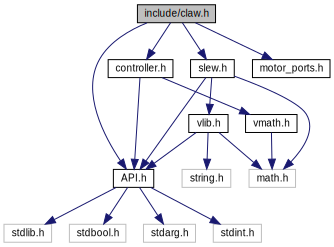
\includegraphics[width=350pt]{claw_8h__incl}
\end{center}
\end{figure}
This graph shows which files directly or indirectly include this file\+:\nopagebreak
\begin{figure}[H]
\begin{center}
\leavevmode
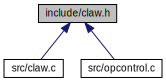
\includegraphics[width=335pt]{claw_8h__dep__incl}
\end{center}
\end{figure}
\subsection*{Macros}
\begin{DoxyCompactItemize}
\item 
\#define \textbf{ C\+L\+A\+W\+\_\+\+C\+L\+O\+SE}~\textbf{ M\+A\+S\+T\+ER}, 6, J\+O\+Y\+\_\+\+UP
\begin{DoxyCompactList}\small\item\em The joystick parameters for closing the claw. \end{DoxyCompactList}\item 
\#define \textbf{ C\+L\+A\+W\+\_\+\+C\+L\+O\+S\+E\+\_\+\+V\+AL}~3000
\begin{DoxyCompactList}\small\item\em The potentiometer value for a closed claw. \end{DoxyCompactList}\item 
\#define \textbf{ C\+L\+A\+W\+\_\+D}~.\+1
\begin{DoxyCompactList}\small\item\em The derivative constant for the claw P\+ID controller. \end{DoxyCompactList}\item 
\#define \textbf{ C\+L\+A\+W\+\_\+I}~0
\begin{DoxyCompactList}\small\item\em The integral constant for the claw P\+ID controller. \end{DoxyCompactList}\item 
\#define \textbf{ C\+L\+A\+W\+\_\+\+O\+P\+EN}~\textbf{ M\+A\+S\+T\+ER}, 6, J\+O\+Y\+\_\+\+D\+O\+WN
\begin{DoxyCompactList}\small\item\em The joystick parameters for opening the claw. \end{DoxyCompactList}\item 
\#define \textbf{ C\+L\+A\+W\+\_\+\+O\+P\+E\+N\+\_\+\+V\+AL}~1500
\begin{DoxyCompactList}\small\item\em The potentiometer value for a open claw. \end{DoxyCompactList}\item 
\#define \textbf{ C\+L\+A\+W\+\_\+P}~.\+1
\begin{DoxyCompactList}\small\item\em The proportional constant for the claw P\+ID controller. \end{DoxyCompactList}\item 
\#define \textbf{ M\+A\+X\+\_\+\+C\+L\+A\+W\+\_\+\+S\+P\+E\+ED}~50
\begin{DoxyCompactList}\small\item\em The max motor vlaue of the claw. \end{DoxyCompactList}\item 
\#define \textbf{ M\+I\+N\+\_\+\+C\+L\+A\+W\+\_\+\+S\+P\+E\+ED}~-\/50
\begin{DoxyCompactList}\small\item\em The min motor vlaue of the claw. \end{DoxyCompactList}\end{DoxyCompactItemize}
\subsection*{Enumerations}
\begin{DoxyCompactItemize}
\item 
enum \textbf{ claw\+\_\+state} \{ \textbf{ C\+L\+A\+W\+\_\+\+O\+P\+E\+N\+\_\+\+S\+T\+A\+TE}, 
\textbf{ C\+L\+A\+W\+\_\+\+C\+L\+O\+S\+E\+\_\+\+S\+T\+A\+TE}
 \}\begin{DoxyCompactList}\small\item\em The different states of the claw. \end{DoxyCompactList}
\end{DoxyCompactItemize}
\subsection*{Functions}
\begin{DoxyCompactItemize}
\item 
void \textbf{ close\+\_\+claw} ()
\begin{DoxyCompactList}\small\item\em Drives the motors to close the claw. \end{DoxyCompactList}\item 
unsigned int \textbf{ get\+Claw\+Ticks} ()
\begin{DoxyCompactList}\small\item\em Gets the claw position in potentiometer ticks. \end{DoxyCompactList}\item 
void \textbf{ open\+\_\+claw} ()
\begin{DoxyCompactList}\small\item\em Drives the motors to open the claw. \end{DoxyCompactList}\item 
void \textbf{ set\+\_\+claw\+\_\+motor} (const int v)
\begin{DoxyCompactList}\small\item\em sets the claw motor speed \end{DoxyCompactList}\item 
void \textbf{ update\+\_\+claw} ()
\begin{DoxyCompactList}\small\item\em Updates the claw motor values. \end{DoxyCompactList}\end{DoxyCompactItemize}


\subsection{Detailed Description}
Code for controlling the claw that grabs the cones. 

\begin{DoxyAuthor}{Author}
Chris Jerrett, Christian Desimone 
\end{DoxyAuthor}
\begin{DoxyDate}{Date}
8/30/2017 
\end{DoxyDate}


Definition in file \textbf{ claw.\+h}.



\subsection{Macro Definition Documentation}
\mbox{\label{claw_8h_af2a18397e9efae0be9470a76797b2077}} 
\index{claw.\+h@{claw.\+h}!C\+L\+A\+W\+\_\+\+C\+L\+O\+SE@{C\+L\+A\+W\+\_\+\+C\+L\+O\+SE}}
\index{C\+L\+A\+W\+\_\+\+C\+L\+O\+SE@{C\+L\+A\+W\+\_\+\+C\+L\+O\+SE}!claw.\+h@{claw.\+h}}
\subsubsection{C\+L\+A\+W\+\_\+\+C\+L\+O\+SE}
{\footnotesize\ttfamily \#define C\+L\+A\+W\+\_\+\+C\+L\+O\+SE~\textbf{ M\+A\+S\+T\+ER}, 6, J\+O\+Y\+\_\+\+UP}



The joystick parameters for closing the claw. 

\begin{DoxyAuthor}{Author}
Chris Jerrett 
\end{DoxyAuthor}


Definition at line \textbf{ 47} of file \textbf{ claw.\+h}.



Referenced by \textbf{ update\+\_\+claw()}.

\mbox{\label{claw_8h_a78d3e6f3d4b60e1be137fdc6dd144224}} 
\index{claw.\+h@{claw.\+h}!C\+L\+A\+W\+\_\+\+C\+L\+O\+S\+E\+\_\+\+V\+AL@{C\+L\+A\+W\+\_\+\+C\+L\+O\+S\+E\+\_\+\+V\+AL}}
\index{C\+L\+A\+W\+\_\+\+C\+L\+O\+S\+E\+\_\+\+V\+AL@{C\+L\+A\+W\+\_\+\+C\+L\+O\+S\+E\+\_\+\+V\+AL}!claw.\+h@{claw.\+h}}
\subsubsection{C\+L\+A\+W\+\_\+\+C\+L\+O\+S\+E\+\_\+\+V\+AL}
{\footnotesize\ttfamily \#define C\+L\+A\+W\+\_\+\+C\+L\+O\+S\+E\+\_\+\+V\+AL~3000}



The potentiometer value for a closed claw. 

\begin{DoxyAuthor}{Author}
Chris Jerrett 
\end{DoxyAuthor}


Definition at line \textbf{ 59} of file \textbf{ claw.\+h}.



Referenced by \textbf{ update\+\_\+claw()}.

\mbox{\label{claw_8h_afa5b4892ddbbfd14068e08422386bc3f}} 
\index{claw.\+h@{claw.\+h}!C\+L\+A\+W\+\_\+D@{C\+L\+A\+W\+\_\+D}}
\index{C\+L\+A\+W\+\_\+D@{C\+L\+A\+W\+\_\+D}!claw.\+h@{claw.\+h}}
\subsubsection{C\+L\+A\+W\+\_\+D}
{\footnotesize\ttfamily \#define C\+L\+A\+W\+\_\+D~.\+1}



The derivative constant for the claw P\+ID controller. 

\begin{DoxyAuthor}{Author}
Chris Jerrett 
\end{DoxyAuthor}


Definition at line \textbf{ 25} of file \textbf{ claw.\+h}.



Referenced by \textbf{ update\+\_\+claw()}.

\mbox{\label{claw_8h_a012d8ac544ee8a7a6413cee1b456773c}} 
\index{claw.\+h@{claw.\+h}!C\+L\+A\+W\+\_\+I@{C\+L\+A\+W\+\_\+I}}
\index{C\+L\+A\+W\+\_\+I@{C\+L\+A\+W\+\_\+I}!claw.\+h@{claw.\+h}}
\subsubsection{C\+L\+A\+W\+\_\+I}
{\footnotesize\ttfamily \#define C\+L\+A\+W\+\_\+I~0}



The integral constant for the claw P\+ID controller. 

\begin{DoxyAuthor}{Author}
Chris Jerrett 
\end{DoxyAuthor}


Definition at line \textbf{ 30} of file \textbf{ claw.\+h}.

\mbox{\label{claw_8h_ae42993ee3f6f4a0e47f99060fe736ba0}} 
\index{claw.\+h@{claw.\+h}!C\+L\+A\+W\+\_\+\+O\+P\+EN@{C\+L\+A\+W\+\_\+\+O\+P\+EN}}
\index{C\+L\+A\+W\+\_\+\+O\+P\+EN@{C\+L\+A\+W\+\_\+\+O\+P\+EN}!claw.\+h@{claw.\+h}}
\subsubsection{C\+L\+A\+W\+\_\+\+O\+P\+EN}
{\footnotesize\ttfamily \#define C\+L\+A\+W\+\_\+\+O\+P\+EN~\textbf{ M\+A\+S\+T\+ER}, 6, J\+O\+Y\+\_\+\+D\+O\+WN}



The joystick parameters for opening the claw. 

\begin{DoxyAuthor}{Author}
Chris Jerrett 
\end{DoxyAuthor}


Definition at line \textbf{ 53} of file \textbf{ claw.\+h}.



Referenced by \textbf{ update\+\_\+claw()}.

\mbox{\label{claw_8h_a519372d8dfa1706d706053ab035ea0b9}} 
\index{claw.\+h@{claw.\+h}!C\+L\+A\+W\+\_\+\+O\+P\+E\+N\+\_\+\+V\+AL@{C\+L\+A\+W\+\_\+\+O\+P\+E\+N\+\_\+\+V\+AL}}
\index{C\+L\+A\+W\+\_\+\+O\+P\+E\+N\+\_\+\+V\+AL@{C\+L\+A\+W\+\_\+\+O\+P\+E\+N\+\_\+\+V\+AL}!claw.\+h@{claw.\+h}}
\subsubsection{C\+L\+A\+W\+\_\+\+O\+P\+E\+N\+\_\+\+V\+AL}
{\footnotesize\ttfamily \#define C\+L\+A\+W\+\_\+\+O\+P\+E\+N\+\_\+\+V\+AL~1500}



The potentiometer value for a open claw. 

\begin{DoxyAuthor}{Author}
Chris Jerrett 
\end{DoxyAuthor}


Definition at line \textbf{ 65} of file \textbf{ claw.\+h}.



Referenced by \textbf{ update\+\_\+claw()}.

\mbox{\label{claw_8h_a1f95cce21c67a6f43850ab9660c2d68a}} 
\index{claw.\+h@{claw.\+h}!C\+L\+A\+W\+\_\+P@{C\+L\+A\+W\+\_\+P}}
\index{C\+L\+A\+W\+\_\+P@{C\+L\+A\+W\+\_\+P}!claw.\+h@{claw.\+h}}
\subsubsection{C\+L\+A\+W\+\_\+P}
{\footnotesize\ttfamily \#define C\+L\+A\+W\+\_\+P~.\+1}



The proportional constant for the claw P\+ID controller. 

\begin{DoxyAuthor}{Author}
Chris Jerrett 
\end{DoxyAuthor}


Definition at line \textbf{ 20} of file \textbf{ claw.\+h}.



Referenced by \textbf{ update\+\_\+claw()}.

\mbox{\label{claw_8h_ae3be50b28977dac719f086e131ba8fd7}} 
\index{claw.\+h@{claw.\+h}!M\+A\+X\+\_\+\+C\+L\+A\+W\+\_\+\+S\+P\+E\+ED@{M\+A\+X\+\_\+\+C\+L\+A\+W\+\_\+\+S\+P\+E\+ED}}
\index{M\+A\+X\+\_\+\+C\+L\+A\+W\+\_\+\+S\+P\+E\+ED@{M\+A\+X\+\_\+\+C\+L\+A\+W\+\_\+\+S\+P\+E\+ED}!claw.\+h@{claw.\+h}}
\subsubsection{M\+A\+X\+\_\+\+C\+L\+A\+W\+\_\+\+S\+P\+E\+ED}
{\footnotesize\ttfamily \#define M\+A\+X\+\_\+\+C\+L\+A\+W\+\_\+\+S\+P\+E\+ED~50}



The max motor vlaue of the claw. 

\begin{DoxyAuthor}{Author}
Chris Jerrett 
\end{DoxyAuthor}


Definition at line \textbf{ 36} of file \textbf{ claw.\+h}.



Referenced by \textbf{ open\+\_\+claw()}.

\mbox{\label{claw_8h_a7306e61a4209c74862aa81d7b3de74e5}} 
\index{claw.\+h@{claw.\+h}!M\+I\+N\+\_\+\+C\+L\+A\+W\+\_\+\+S\+P\+E\+ED@{M\+I\+N\+\_\+\+C\+L\+A\+W\+\_\+\+S\+P\+E\+ED}}
\index{M\+I\+N\+\_\+\+C\+L\+A\+W\+\_\+\+S\+P\+E\+ED@{M\+I\+N\+\_\+\+C\+L\+A\+W\+\_\+\+S\+P\+E\+ED}!claw.\+h@{claw.\+h}}
\subsubsection{M\+I\+N\+\_\+\+C\+L\+A\+W\+\_\+\+S\+P\+E\+ED}
{\footnotesize\ttfamily \#define M\+I\+N\+\_\+\+C\+L\+A\+W\+\_\+\+S\+P\+E\+ED~-\/50}



The min motor vlaue of the claw. 

\begin{DoxyAuthor}{Author}
Chris Jerrett 
\end{DoxyAuthor}


Definition at line \textbf{ 41} of file \textbf{ claw.\+h}.



Referenced by \textbf{ close\+\_\+claw()}.



\subsection{Enumeration Type Documentation}
\mbox{\label{claw_8h_a600668fd307d596c3812126657335324}} 
\index{claw.\+h@{claw.\+h}!claw\+\_\+state@{claw\+\_\+state}}
\index{claw\+\_\+state@{claw\+\_\+state}!claw.\+h@{claw.\+h}}
\subsubsection{claw\+\_\+state}
{\footnotesize\ttfamily enum \textbf{ claw\+\_\+state}}



The different states of the claw. 

\begin{DoxyAuthor}{Author}
Chris Jerrett 
\end{DoxyAuthor}
\begin{DoxyEnumFields}{Enumerator}
\raisebox{\heightof{T}}[0pt][0pt]{\index{C\+L\+A\+W\+\_\+\+O\+P\+E\+N\+\_\+\+S\+T\+A\+TE@{C\+L\+A\+W\+\_\+\+O\+P\+E\+N\+\_\+\+S\+T\+A\+TE}!claw.\+h@{claw.\+h}}\index{claw.\+h@{claw.\+h}!C\+L\+A\+W\+\_\+\+O\+P\+E\+N\+\_\+\+S\+T\+A\+TE@{C\+L\+A\+W\+\_\+\+O\+P\+E\+N\+\_\+\+S\+T\+A\+TE}}}\mbox{\label{claw_8h_a600668fd307d596c3812126657335324ab871ce9ec2796d275c09bf01abcac2cd}} 
C\+L\+A\+W\+\_\+\+O\+P\+E\+N\+\_\+\+S\+T\+A\+TE&\\
\hline

\raisebox{\heightof{T}}[0pt][0pt]{\index{C\+L\+A\+W\+\_\+\+C\+L\+O\+S\+E\+\_\+\+S\+T\+A\+TE@{C\+L\+A\+W\+\_\+\+C\+L\+O\+S\+E\+\_\+\+S\+T\+A\+TE}!claw.\+h@{claw.\+h}}\index{claw.\+h@{claw.\+h}!C\+L\+A\+W\+\_\+\+C\+L\+O\+S\+E\+\_\+\+S\+T\+A\+TE@{C\+L\+A\+W\+\_\+\+C\+L\+O\+S\+E\+\_\+\+S\+T\+A\+TE}}}\mbox{\label{claw_8h_a600668fd307d596c3812126657335324a3948a2d760f710e9087edded3df98b5f}} 
C\+L\+A\+W\+\_\+\+C\+L\+O\+S\+E\+\_\+\+S\+T\+A\+TE&\\
\hline

\end{DoxyEnumFields}


Definition at line \textbf{ 101} of file \textbf{ claw.\+h}.


\begin{DoxyCode}
00101                 \{
00102   CLAW_OPEN_STATE,
00103   CLAW_CLOSE_STATE
00104 \};
\end{DoxyCode}


\subsection{Function Documentation}
\mbox{\label{claw_8h_ac42dd40dbb37219295286859c6b068c2}} 
\index{claw.\+h@{claw.\+h}!close\+\_\+claw@{close\+\_\+claw}}
\index{close\+\_\+claw@{close\+\_\+claw}!claw.\+h@{claw.\+h}}
\subsubsection{close\+\_\+claw()}
{\footnotesize\ttfamily void close\+\_\+claw (\begin{DoxyParamCaption}{ }\end{DoxyParamCaption})}



Drives the motors to close the claw. 

\begin{DoxyAuthor}{Author}
Chris Jerrett 
\end{DoxyAuthor}


Definition at line \textbf{ 67} of file \textbf{ claw.\+c}.



References \textbf{ C\+L\+A\+W\+\_\+\+M\+O\+T\+OR}, \textbf{ M\+I\+N\+\_\+\+C\+L\+A\+W\+\_\+\+S\+P\+E\+ED}, and \textbf{ set\+\_\+motor\+\_\+immediate()}.



Referenced by \textbf{ autonomous()}.


\begin{DoxyCode}
00067                   \{
00068   set_motor_immediate(CLAW_MOTOR, MIN_CLAW_SPEED);
00069 \}
\end{DoxyCode}
\mbox{\label{claw_8h_addd2004effae7c94400aed1fe6a90ead}} 
\index{claw.\+h@{claw.\+h}!get\+Claw\+Ticks@{get\+Claw\+Ticks}}
\index{get\+Claw\+Ticks@{get\+Claw\+Ticks}!claw.\+h@{claw.\+h}}
\subsubsection{get\+Claw\+Ticks()}
{\footnotesize\ttfamily unsigned int get\+Claw\+Ticks (\begin{DoxyParamCaption}{ }\end{DoxyParamCaption})}



Gets the claw position in potentiometer ticks. 

\begin{DoxyAuthor}{Author}
Chris Jerrett 
\end{DoxyAuthor}


Definition at line \textbf{ 51} of file \textbf{ claw.\+c}.



References \textbf{ C\+L\+A\+W\+\_\+\+P\+OT}.



Referenced by \textbf{ update\+\_\+claw()}.


\begin{DoxyCode}
00051                            \{
00052   \textcolor{keywordflow}{return} analogRead(CLAW_POT);
00053 \}
\end{DoxyCode}
\mbox{\label{claw_8h_a03023ca28f671b9fa7bac07782ccd8c1}} 
\index{claw.\+h@{claw.\+h}!open\+\_\+claw@{open\+\_\+claw}}
\index{open\+\_\+claw@{open\+\_\+claw}!claw.\+h@{claw.\+h}}
\subsubsection{open\+\_\+claw()}
{\footnotesize\ttfamily void open\+\_\+claw (\begin{DoxyParamCaption}{ }\end{DoxyParamCaption})}



Drives the motors to open the claw. 

\begin{DoxyAuthor}{Author}
Chris Jerrett 
\end{DoxyAuthor}


Definition at line \textbf{ 59} of file \textbf{ claw.\+c}.



References \textbf{ C\+L\+A\+W\+\_\+\+M\+O\+T\+OR}, \textbf{ M\+A\+X\+\_\+\+C\+L\+A\+W\+\_\+\+S\+P\+E\+ED}, and \textbf{ set\+\_\+motor\+\_\+immediate()}.



Referenced by \textbf{ autonomous()}.


\begin{DoxyCode}
00059                  \{
00060   set_motor_immediate(CLAW_MOTOR, MAX_CLAW_SPEED);
00061 \}
\end{DoxyCode}
\mbox{\label{claw_8h_a3a57f998b1884d39b0cc786689f7086f}} 
\index{claw.\+h@{claw.\+h}!set\+\_\+claw\+\_\+motor@{set\+\_\+claw\+\_\+motor}}
\index{set\+\_\+claw\+\_\+motor@{set\+\_\+claw\+\_\+motor}!claw.\+h@{claw.\+h}}
\subsubsection{set\+\_\+claw\+\_\+motor()}
{\footnotesize\ttfamily void set\+\_\+claw\+\_\+motor (\begin{DoxyParamCaption}\item[{const int}]{v }\end{DoxyParamCaption})}



sets the claw motor speed 

\begin{DoxyAuthor}{Author}
Chris Jerrett 
\end{DoxyAuthor}


Definition at line \textbf{ 43} of file \textbf{ claw.\+c}.



References \textbf{ C\+L\+A\+W\+\_\+\+M\+O\+T\+OR}, and \textbf{ set\+\_\+motor\+\_\+immediate()}.



Referenced by \textbf{ update\+\_\+claw()}.


\begin{DoxyCode}
00043                                 \{
00044   set_motor_immediate(CLAW_MOTOR, v);
00045 \}
\end{DoxyCode}
\mbox{\label{claw_8h_a0122b78972344264b8a276a559cfce4a}} 
\index{claw.\+h@{claw.\+h}!update\+\_\+claw@{update\+\_\+claw}}
\index{update\+\_\+claw@{update\+\_\+claw}!claw.\+h@{claw.\+h}}
\subsubsection{update\+\_\+claw()}
{\footnotesize\ttfamily void update\+\_\+claw (\begin{DoxyParamCaption}{ }\end{DoxyParamCaption})}



Updates the claw motor values. 

\begin{DoxyAuthor}{Author}
Chris Jerrett 
\end{DoxyAuthor}


Definition at line \textbf{ 7} of file \textbf{ claw.\+c}.



References \textbf{ C\+L\+A\+W\+\_\+\+C\+L\+O\+SE}, \textbf{ C\+L\+A\+W\+\_\+\+C\+L\+O\+S\+E\+\_\+\+S\+T\+A\+TE}, \textbf{ C\+L\+A\+W\+\_\+\+C\+L\+O\+S\+E\+\_\+\+V\+AL}, \textbf{ C\+L\+A\+W\+\_\+D}, \textbf{ C\+L\+A\+W\+\_\+\+O\+P\+EN}, \textbf{ C\+L\+A\+W\+\_\+\+O\+P\+E\+N\+\_\+\+S\+T\+A\+TE}, \textbf{ C\+L\+A\+W\+\_\+\+O\+P\+E\+N\+\_\+\+V\+AL}, \textbf{ C\+L\+A\+W\+\_\+P}, \textbf{ get\+Claw\+Ticks()}, and \textbf{ set\+\_\+claw\+\_\+motor()}.



Referenced by \textbf{ operator\+Control()}.


\begin{DoxyCode}
00007                    \{
00008   \textcolor{comment}{//Set the Error used in calculating d}
00009   \textcolor{keyword}{static} \textcolor{keywordtype}{int} last\_error = 0;
00010   \textcolor{comment}{//Set the initial claw state to open}
00011   \textcolor{keyword}{static} \textcolor{keyword}{enum} claw_state state = CLAW_OPEN_STATE;
00012   \textcolor{comment}{//Listen for input and either close or open the claw}
00013   \textcolor{keywordflow}{if}(joystickGetDigital(CLAW_CLOSE))\{
00014     state = CLAW_CLOSE_STATE;
00015   \}
00016   \textcolor{keywordflow}{else} \textcolor{keywordflow}{if}(joystickGetDigital(CLAW_OPEN))\{
00017     state = CLAW_OPEN_STATE;
00018   \} \textcolor{keywordflow}{else} \{
00019     \textcolor{comment}{//set the default motor speed}
00020     \textcolor{keywordtype}{int} p = 0;
00021     \textcolor{comment}{//Change the base speed to the difference between the target}
00022     \textcolor{comment}{// and the current value}
00023     \textcolor{keywordflow}{if}(state == CLAW_OPEN_STATE) \{
00024       p = getClawTicks() - CLAW_OPEN_VAL;
00025     \} \textcolor{keywordflow}{else} \{
00026       p = getClawTicks() - CLAW_CLOSE_VAL;
00027     \}
00028     \textcolor{comment}{//Set the d value to the difference between the current p and the last p}
00029     \textcolor{keywordtype}{int} d = (p - last\_error);
00030     \textcolor{comment}{//Set last error for use the next time the function is run}
00031     last\_error = p;
00032     \textcolor{comment}{//Construct the final motor speed value}
00033     \textcolor{keywordtype}{int} motor = CLAW_P * p + CLAW_D * d;
00034     \textcolor{comment}{//Set the motor speed}
00035     set_claw_motor(motor);
00036   \}
00037 \}
\end{DoxyCode}

\section{claw.\+h}
\label{claw_8h_source}\index{include/claw.\+h@{include/claw.\+h}}

\begin{DoxyCode}
00001 
00007 \textcolor{preprocessor}{#ifndef \_CLAW\_H\_}
00008 \textcolor{preprocessor}{#define \_CLAW\_H\_}
00009 
00010 \textcolor{preprocessor}{#include "slew.h"}
00011 \textcolor{preprocessor}{#include <API.h>}
00012 \textcolor{preprocessor}{#include "controller.h"}
00013 \textcolor{preprocessor}{#include "motor_ports.h"}
00014 \textcolor{preprocessor}{#include "sensor_ports.h"}
00015 
00020 \textcolor{preprocessor}{#define CLAW\_P .1}
00021 
00025 \textcolor{preprocessor}{#define CLAW\_D .1}
00026 
00030 \textcolor{preprocessor}{#define CLAW\_I 0}
00031 
00036 \textcolor{preprocessor}{#define MAX\_CLAW\_SPEED 50}
00037 
00041 \textcolor{preprocessor}{#define MIN\_CLAW\_SPEED -50}
00042 
00047 \textcolor{preprocessor}{#define CLAW\_CLOSE MASTER, 6, JOY\_UP}
00048 
00053 \textcolor{preprocessor}{#define CLAW\_OPEN MASTER, 6, JOY\_DOWN}
00054 
00059 \textcolor{preprocessor}{#define CLAW\_CLOSE\_VAL 3000}
00060 
00065 \textcolor{preprocessor}{#define CLAW\_OPEN\_VAL 1500}
00066 
00071 \textcolor{keywordtype}{void} update_claw();
00072 
00077 \textcolor{keywordtype}{void} set_claw_motor(\textcolor{keyword}{const} \textcolor{keywordtype}{int} v);
00078 
00083 \textcolor{keywordtype}{unsigned} \textcolor{keywordtype}{int} getClawTicks();
00084 
00089 \textcolor{keywordtype}{void} open_claw();
00090 
00095 \textcolor{keywordtype}{void} close_claw();
00096 
00101 \textcolor{keyword}{enum} claw_state \{
00102   CLAW_OPEN_STATE,
00103   CLAW_CLOSE_STATE
00104 \};
00105 
00106 \textcolor{preprocessor}{#endif}
\end{DoxyCode}

\section{include/controller.h File Reference}
\label{controller_8h}\index{include/controller.\+h@{include/controller.\+h}}


controller definitions, macros and functions to assist with usig the vex controllers.  


{\ttfamily \#include \char`\"{}vmath.\+h\char`\"{}}\newline
{\ttfamily \#include $<$A\+P\+I.\+h$>$}\newline
Include dependency graph for controller.\+h\+:\nopagebreak
\begin{figure}[H]
\begin{center}
\leavevmode
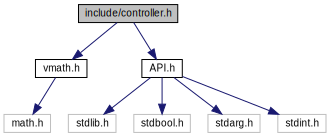
\includegraphics[width=190pt]{controller_8h__incl}
\end{center}
\end{figure}
This graph shows which files directly or indirectly include this file\+:\nopagebreak
\begin{figure}[H]
\begin{center}
\leavevmode
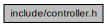
\includegraphics[width=350pt]{controller_8h__dep__incl}
\end{center}
\end{figure}
\subsection*{Macros}
\begin{DoxyCompactItemize}
\item 
\#define \textbf{ L\+E\+F\+T\+\_\+\+B\+U\+M\+P\+E\+RS}~6
\item 
\#define \textbf{ L\+E\+F\+T\+\_\+\+B\+U\+T\+T\+O\+NS}~7
\item 
\#define \textbf{ L\+E\+F\+T\+\_\+\+J\+O\+Y\+\_\+X}~4
\begin{DoxyCompactList}\small\item\em the left x joystick on controller \end{DoxyCompactList}\item 
\#define \textbf{ L\+E\+F\+T\+\_\+\+J\+O\+Y\+\_\+Y}~3
\begin{DoxyCompactList}\small\item\em the left y joystick on controller \end{DoxyCompactList}\item 
\#define \textbf{ M\+A\+S\+T\+ER}~1
\begin{DoxyCompactList}\small\item\em the master controller \end{DoxyCompactList}\item 
\#define \textbf{ P\+A\+R\+T\+N\+ER}~2
\begin{DoxyCompactList}\small\item\em the slave/partner controller \end{DoxyCompactList}\item 
\#define \textbf{ R\+I\+G\+H\+T\+\_\+\+B\+U\+M\+P\+E\+RS}~5
\item 
\#define \textbf{ R\+I\+G\+H\+T\+\_\+\+B\+U\+T\+T\+O\+NS}~8
\item 
\#define \textbf{ R\+I\+G\+H\+T\+\_\+\+J\+O\+Y\+\_\+X}~1
\begin{DoxyCompactList}\small\item\em the right x joystick on controller \end{DoxyCompactList}\item 
\#define \textbf{ R\+I\+G\+H\+T\+\_\+\+J\+O\+Y\+\_\+Y}~2
\begin{DoxyCompactList}\small\item\em the right y joystick on controller \end{DoxyCompactList}\end{DoxyCompactItemize}
\subsection*{Enumerations}
\begin{DoxyCompactItemize}
\item 
enum \textbf{ joystick} \{ \textbf{ R\+I\+G\+H\+T\+\_\+\+J\+OY}, 
\textbf{ L\+E\+F\+T\+\_\+\+J\+OY}
 \}\begin{DoxyCompactList}\small\item\em Represents a joystick on the controller. \end{DoxyCompactList}
\end{DoxyCompactItemize}
\subsection*{Functions}
\begin{DoxyCompactItemize}
\item 
struct \textbf{ cord} \textbf{ get\+\_\+joystick\+\_\+cord} (enum \textbf{ joystick} \textbf{ side}, int controller)
\begin{DoxyCompactList}\small\item\em Gets the location of a joystick on the controller. \end{DoxyCompactList}\end{DoxyCompactItemize}


\subsection{Detailed Description}
controller definitions, macros and functions to assist with usig the vex controllers. 

\begin{DoxyAuthor}{Author}
Chris Jerrett, Christian Desimone 
\end{DoxyAuthor}
\begin{DoxyDate}{Date}
9/9/2017 
\end{DoxyDate}


Definition in file \textbf{ controller.\+h}.



\subsection{Macro Definition Documentation}
\mbox{\label{controller_8h_ad61eb6d28a76985afb8d39ef925541bb}} 
\index{controller.\+h@{controller.\+h}!L\+E\+F\+T\+\_\+\+B\+U\+M\+P\+E\+RS@{L\+E\+F\+T\+\_\+\+B\+U\+M\+P\+E\+RS}}
\index{L\+E\+F\+T\+\_\+\+B\+U\+M\+P\+E\+RS@{L\+E\+F\+T\+\_\+\+B\+U\+M\+P\+E\+RS}!controller.\+h@{controller.\+h}}
\subsubsection{L\+E\+F\+T\+\_\+\+B\+U\+M\+P\+E\+RS}
{\footnotesize\ttfamily \#define L\+E\+F\+T\+\_\+\+B\+U\+M\+P\+E\+RS~6}



Definition at line \textbf{ 18} of file \textbf{ controller.\+h}.

\mbox{\label{controller_8h_a9b885de9f143efd0c862ceb054256536}} 
\index{controller.\+h@{controller.\+h}!L\+E\+F\+T\+\_\+\+B\+U\+T\+T\+O\+NS@{L\+E\+F\+T\+\_\+\+B\+U\+T\+T\+O\+NS}}
\index{L\+E\+F\+T\+\_\+\+B\+U\+T\+T\+O\+NS@{L\+E\+F\+T\+\_\+\+B\+U\+T\+T\+O\+NS}!controller.\+h@{controller.\+h}}
\subsubsection{L\+E\+F\+T\+\_\+\+B\+U\+T\+T\+O\+NS}
{\footnotesize\ttfamily \#define L\+E\+F\+T\+\_\+\+B\+U\+T\+T\+O\+NS~7}



Definition at line \textbf{ 16} of file \textbf{ controller.\+h}.

\mbox{\label{controller_8h_ac055a23829dc64aa20b8e2e1bcfbf316}} 
\index{controller.\+h@{controller.\+h}!L\+E\+F\+T\+\_\+\+J\+O\+Y\+\_\+X@{L\+E\+F\+T\+\_\+\+J\+O\+Y\+\_\+X}}
\index{L\+E\+F\+T\+\_\+\+J\+O\+Y\+\_\+X@{L\+E\+F\+T\+\_\+\+J\+O\+Y\+\_\+X}!controller.\+h@{controller.\+h}}
\subsubsection{L\+E\+F\+T\+\_\+\+J\+O\+Y\+\_\+X}
{\footnotesize\ttfamily \#define L\+E\+F\+T\+\_\+\+J\+O\+Y\+\_\+X~4}



the left x joystick on controller 

\begin{DoxyDate}{Date}
9/1/2017 
\end{DoxyDate}
\begin{DoxyAuthor}{Author}
Chris Jerrett 
\end{DoxyAuthor}


Definition at line \textbf{ 53} of file \textbf{ controller.\+h}.



Referenced by \textbf{ get\+\_\+joystick\+\_\+cord()}.

\mbox{\label{controller_8h_ae0a2b64db5fc4f4bf4b169185be93db3}} 
\index{controller.\+h@{controller.\+h}!L\+E\+F\+T\+\_\+\+J\+O\+Y\+\_\+Y@{L\+E\+F\+T\+\_\+\+J\+O\+Y\+\_\+Y}}
\index{L\+E\+F\+T\+\_\+\+J\+O\+Y\+\_\+Y@{L\+E\+F\+T\+\_\+\+J\+O\+Y\+\_\+Y}!controller.\+h@{controller.\+h}}
\subsubsection{L\+E\+F\+T\+\_\+\+J\+O\+Y\+\_\+Y}
{\footnotesize\ttfamily \#define L\+E\+F\+T\+\_\+\+J\+O\+Y\+\_\+Y~3}



the left y joystick on controller 

\begin{DoxyDate}{Date}
9/1/2017 
\end{DoxyDate}
\begin{DoxyAuthor}{Author}
Chris Jerrett 
\end{DoxyAuthor}


Definition at line \textbf{ 60} of file \textbf{ controller.\+h}.



Referenced by \textbf{ get\+\_\+joystick\+\_\+cord()}.

\mbox{\label{controller_8h_a3fa2d3bf1901157f734a584d47b25d8b}} 
\index{controller.\+h@{controller.\+h}!M\+A\+S\+T\+ER@{M\+A\+S\+T\+ER}}
\index{M\+A\+S\+T\+ER@{M\+A\+S\+T\+ER}!controller.\+h@{controller.\+h}}
\subsubsection{M\+A\+S\+T\+ER}
{\footnotesize\ttfamily \#define M\+A\+S\+T\+ER~1}



the master controller 

\begin{DoxyDate}{Date}
9/1/2017 
\end{DoxyDate}
\begin{DoxyAuthor}{Author}
Chris Jerrett 
\end{DoxyAuthor}


Definition at line \textbf{ 25} of file \textbf{ controller.\+h}.



Referenced by \textbf{ update\+\_\+drive\+\_\+motors()}, and \textbf{ update\+Intake()}.

\mbox{\label{controller_8h_a136e64cf351535da81cacb6a546cade6}} 
\index{controller.\+h@{controller.\+h}!P\+A\+R\+T\+N\+ER@{P\+A\+R\+T\+N\+ER}}
\index{P\+A\+R\+T\+N\+ER@{P\+A\+R\+T\+N\+ER}!controller.\+h@{controller.\+h}}
\subsubsection{P\+A\+R\+T\+N\+ER}
{\footnotesize\ttfamily \#define P\+A\+R\+T\+N\+ER~2}



the slave/partner controller 

\begin{DoxyDate}{Date}
9/1/2017 
\end{DoxyDate}
\begin{DoxyAuthor}{Author}
Chris Jerrett 
\end{DoxyAuthor}


Definition at line \textbf{ 32} of file \textbf{ controller.\+h}.



Referenced by \textbf{ update\+\_\+control()}, \textbf{ update\+\_\+drive\+\_\+motors()}, and \textbf{ update\+Intake()}.

\mbox{\label{controller_8h_a635896b08789914290171051d1b82465}} 
\index{controller.\+h@{controller.\+h}!R\+I\+G\+H\+T\+\_\+\+B\+U\+M\+P\+E\+RS@{R\+I\+G\+H\+T\+\_\+\+B\+U\+M\+P\+E\+RS}}
\index{R\+I\+G\+H\+T\+\_\+\+B\+U\+M\+P\+E\+RS@{R\+I\+G\+H\+T\+\_\+\+B\+U\+M\+P\+E\+RS}!controller.\+h@{controller.\+h}}
\subsubsection{R\+I\+G\+H\+T\+\_\+\+B\+U\+M\+P\+E\+RS}
{\footnotesize\ttfamily \#define R\+I\+G\+H\+T\+\_\+\+B\+U\+M\+P\+E\+RS~5}



Definition at line \textbf{ 17} of file \textbf{ controller.\+h}.

\mbox{\label{controller_8h_a68881b6085c880930037b20764fe5aee}} 
\index{controller.\+h@{controller.\+h}!R\+I\+G\+H\+T\+\_\+\+B\+U\+T\+T\+O\+NS@{R\+I\+G\+H\+T\+\_\+\+B\+U\+T\+T\+O\+NS}}
\index{R\+I\+G\+H\+T\+\_\+\+B\+U\+T\+T\+O\+NS@{R\+I\+G\+H\+T\+\_\+\+B\+U\+T\+T\+O\+NS}!controller.\+h@{controller.\+h}}
\subsubsection{R\+I\+G\+H\+T\+\_\+\+B\+U\+T\+T\+O\+NS}
{\footnotesize\ttfamily \#define R\+I\+G\+H\+T\+\_\+\+B\+U\+T\+T\+O\+NS~8}



Definition at line \textbf{ 15} of file \textbf{ controller.\+h}.

\mbox{\label{controller_8h_ad74f84aad465437cc1e0f914dbd6fab5}} 
\index{controller.\+h@{controller.\+h}!R\+I\+G\+H\+T\+\_\+\+J\+O\+Y\+\_\+X@{R\+I\+G\+H\+T\+\_\+\+J\+O\+Y\+\_\+X}}
\index{R\+I\+G\+H\+T\+\_\+\+J\+O\+Y\+\_\+X@{R\+I\+G\+H\+T\+\_\+\+J\+O\+Y\+\_\+X}!controller.\+h@{controller.\+h}}
\subsubsection{R\+I\+G\+H\+T\+\_\+\+J\+O\+Y\+\_\+X}
{\footnotesize\ttfamily \#define R\+I\+G\+H\+T\+\_\+\+J\+O\+Y\+\_\+X~1}



the right x joystick on controller 

\begin{DoxyDate}{Date}
9/1/2017 
\end{DoxyDate}
\begin{DoxyAuthor}{Author}
Chris Jerrett 
\end{DoxyAuthor}


Definition at line \textbf{ 39} of file \textbf{ controller.\+h}.



Referenced by \textbf{ get\+\_\+joystick\+\_\+cord()}.

\mbox{\label{controller_8h_a99457bf9dee795334411ea77f0858b16}} 
\index{controller.\+h@{controller.\+h}!R\+I\+G\+H\+T\+\_\+\+J\+O\+Y\+\_\+Y@{R\+I\+G\+H\+T\+\_\+\+J\+O\+Y\+\_\+Y}}
\index{R\+I\+G\+H\+T\+\_\+\+J\+O\+Y\+\_\+Y@{R\+I\+G\+H\+T\+\_\+\+J\+O\+Y\+\_\+Y}!controller.\+h@{controller.\+h}}
\subsubsection{R\+I\+G\+H\+T\+\_\+\+J\+O\+Y\+\_\+Y}
{\footnotesize\ttfamily \#define R\+I\+G\+H\+T\+\_\+\+J\+O\+Y\+\_\+Y~2}



the right y joystick on controller 

\begin{DoxyDate}{Date}
9/1/2017 
\end{DoxyDate}
\begin{DoxyAuthor}{Author}
Chris Jerrett 
\end{DoxyAuthor}


Definition at line \textbf{ 46} of file \textbf{ controller.\+h}.



Referenced by \textbf{ get\+\_\+joystick\+\_\+cord()}.



\subsection{Enumeration Type Documentation}
\mbox{\label{controller_8h_ac365c9e892abe4a1b85ae8f56a4eae5a}} 
\index{controller.\+h@{controller.\+h}!joystick@{joystick}}
\index{joystick@{joystick}!controller.\+h@{controller.\+h}}
\subsubsection{joystick}
{\footnotesize\ttfamily enum \textbf{ joystick}}



Represents a joystick on the controller. 

\begin{DoxyDate}{Date}
9/10/2017 
\end{DoxyDate}
\begin{DoxyAuthor}{Author}
Chris Jerrett 
\end{DoxyAuthor}
\begin{DoxyEnumFields}{Enumerator}
\raisebox{\heightof{T}}[0pt][0pt]{\index{R\+I\+G\+H\+T\+\_\+\+J\+OY@{R\+I\+G\+H\+T\+\_\+\+J\+OY}!controller.\+h@{controller.\+h}}\index{controller.\+h@{controller.\+h}!R\+I\+G\+H\+T\+\_\+\+J\+OY@{R\+I\+G\+H\+T\+\_\+\+J\+OY}}}\mbox{\label{controller_8h_ac365c9e892abe4a1b85ae8f56a4eae5aae08a2d362c677f96f72d93047513cafe}} 
R\+I\+G\+H\+T\+\_\+\+J\+OY&The right joystick \\
\hline

\raisebox{\heightof{T}}[0pt][0pt]{\index{L\+E\+F\+T\+\_\+\+J\+OY@{L\+E\+F\+T\+\_\+\+J\+OY}!controller.\+h@{controller.\+h}}\index{controller.\+h@{controller.\+h}!L\+E\+F\+T\+\_\+\+J\+OY@{L\+E\+F\+T\+\_\+\+J\+OY}}}\mbox{\label{controller_8h_ac365c9e892abe4a1b85ae8f56a4eae5aaf822d7888862e67a3c624775b85c50a9}} 
L\+E\+F\+T\+\_\+\+J\+OY&The left joystick \\
\hline

\end{DoxyEnumFields}


Definition at line \textbf{ 67} of file \textbf{ controller.\+h}.


\begin{DoxyCode}
00067               \{
00069   RIGHT_JOY,
00071   LEFT_JOY,
00072 \};
\end{DoxyCode}


\subsection{Function Documentation}
\mbox{\label{controller_8h_a0ce0176099c0bb15ad8c36123222059d}} 
\index{controller.\+h@{controller.\+h}!get\+\_\+joystick\+\_\+cord@{get\+\_\+joystick\+\_\+cord}}
\index{get\+\_\+joystick\+\_\+cord@{get\+\_\+joystick\+\_\+cord}!controller.\+h@{controller.\+h}}
\subsubsection{get\+\_\+joystick\+\_\+cord()}
{\footnotesize\ttfamily struct \textbf{ cord} get\+\_\+joystick\+\_\+cord (\begin{DoxyParamCaption}\item[{enum \textbf{ joystick}}]{side,  }\item[{int}]{controller }\end{DoxyParamCaption})}



Gets the location of a joystick on the controller. 

\begin{DoxyAuthor}{Author}
Chris Jerrett 
\end{DoxyAuthor}


Definition at line \textbf{ 7} of file \textbf{ controller.\+c}.



References \textbf{ L\+E\+F\+T\+\_\+\+J\+O\+Y\+\_\+X}, \textbf{ L\+E\+F\+T\+\_\+\+J\+O\+Y\+\_\+Y}, \textbf{ R\+I\+G\+H\+T\+\_\+\+J\+OY}, \textbf{ R\+I\+G\+H\+T\+\_\+\+J\+O\+Y\+\_\+X}, \textbf{ R\+I\+G\+H\+T\+\_\+\+J\+O\+Y\+\_\+Y}, \textbf{ cord\+::x}, and \textbf{ cord\+::y}.


\begin{DoxyCode}
00007                                                                   \{
00008   \textcolor{keywordtype}{int} x;
00009   \textcolor{keywordtype}{int} y;
00010   \textcolor{comment}{//Get the joystick value for either the right or left,}
00011   \textcolor{comment}{//depending on the mode}
00012   \textcolor{keywordflow}{if}(side == RIGHT_JOY) \{
00013     y = joystickGetAnalog(controller, RIGHT_JOY_X);
00014     x = joystickGetAnalog(controller, RIGHT_JOY_Y);
00015   \} \textcolor{keywordflow}{else} \{
00016     y = joystickGetAnalog(controller, LEFT_JOY_X);
00017     x = joystickGetAnalog(controller, LEFT_JOY_Y);
00018   \}
00019   \textcolor{comment}{//Define a coordinate for the joystick value}
00020   \textcolor{keyword}{struct }cord c;
00021   c.x = x;
00022   c.y = y;
00023   \textcolor{keywordflow}{return} c;
00024 \}
\end{DoxyCode}

\subsection{controller.\+h}
\label{controller_8h_source}\index{include/controller.\+h@{include/controller.\+h}}

\begin{DoxyCode}
00001 
00009 \textcolor{preprocessor}{#ifndef \_CONTROLLER\_H\_}
00010 \textcolor{preprocessor}{#define \_CONTROLLER\_H\_}
00011 
00012 \textcolor{preprocessor}{#include "vmath.h"}
00013 \textcolor{preprocessor}{#include <API.h>}
00014 
00015 \textcolor{preprocessor}{#define RIGHT\_BUTTONS 8}
00016 \textcolor{preprocessor}{#define LEFT\_BUTTONS 7}
00017 \textcolor{preprocessor}{#define RIGHT\_BUMPERS 5}
00018 \textcolor{preprocessor}{#define LEFT\_BUMPERS 6}
00019 
00023 \textcolor{keyword}{typedef} \textcolor{keyword}{enum} \{
00024   JOY1_5D = 0,
00025   JOY1_5U = 1,
00026   JOY1_6D = 2,
00027   JOY1_6U = 3,
00028   JOY1_7U = 4,
00029   JOY1_7L = 5,
00030   JOY1_7R = 6,
00031   JOY1_7D = 7,
00032   JOY1_8U = 8,
00033   JOY1_8L = 9,
00034   JOY1_8R = 10,
00035   JOY1_8D = 11,
00036 
00037   JOY2_5D = 12,
00038   JOY2_5U = 13,
00039   JOY2_6D = 14,
00040   JOY2_6U = 15,
00041   JOY2_7U = 16,
00042   JOY2_7L = 17,
00043   JOY2_7R = 18,
00044   JOY2_7D = 19,
00045   JOY2_8U = 20,
00046   JOY2_8L = 21,
00047   JOY2_8R = 22,
00048   JOY2_8D = 23,
00049 
00050   LCD_LEFT = 24,
00051   LCD_CENT = 25,
00052   LCD_RIGHT = 26
00053 \} button_t;
00054 
00060 \textcolor{preprocessor}{#define MASTER 1}
00061 
00067 \textcolor{preprocessor}{#define PARTNER 2}
00068 
00074 \textcolor{preprocessor}{#define RIGHT\_JOY\_X 1}
00075 
00081 \textcolor{preprocessor}{#define RIGHT\_JOY\_Y 2}
00082 
00088 \textcolor{preprocessor}{#define LEFT\_JOY\_X 4}
00089 
00095 \textcolor{preprocessor}{#define LEFT\_JOY\_Y 3}
00096 
00102 \textcolor{keyword}{enum} joystick \{
00104   RIGHT_JOY,
00106   LEFT_JOY,
00107 \};
00108 
00113 \textcolor{keyword}{struct }cord get_joystick_cord(enum joystick side, int controller);
00114 
00115 \textcolor{preprocessor}{#endif}
\end{DoxyCode}

\hypertarget{drive_8h}{}\section{include/drive.h File Reference}
\label{drive_8h}\index{include/drive.\+h@{include/drive.\+h}}


Drive base definitions and enumerations.  


{\ttfamily \#include $<$A\+P\+I.\+h$>$}\newline
{\ttfamily \#include \char`\"{}partner.\+h\char`\"{}}\newline
Include dependency graph for drive.\+h\+:\nopagebreak
\begin{figure}[H]
\begin{center}
\leavevmode
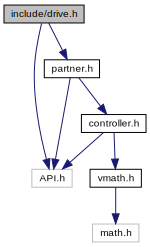
\includegraphics[width=350pt]{drive_8h__incl}
\end{center}
\end{figure}
This graph shows which files directly or indirectly include this file\+:\nopagebreak
\begin{figure}[H]
\begin{center}
\leavevmode
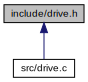
\includegraphics[width=350pt]{drive_8h__dep__incl}
\end{center}
\end{figure}
\subsection*{Macros}
\begin{DoxyCompactItemize}
\item 
\#define \hyperlink{drive_8h_a3d683c4ec93ad778fc5914cd5671a793}{D\+E\+A\+D\+S\+P\+OT}~10
\item 
\#define \hyperlink{drive_8h_a4679d8ea8690999a6c6c7c0cb245c879}{T\+H\+R\+E\+S\+H\+O\+LD}~10
\end{DoxyCompactItemize}
\subsection*{Typedefs}
\begin{DoxyCompactItemize}
\item 
typedef enum \hyperlink{drive_8h_afc015eff6557e84151d2e53b94375445}{side} \hyperlink{drive_8h_a9df2afd2f1acb97019655e5e730609c7}{side\+\_\+t}
\begin{DoxyCompactList}\small\item\em enumeration indication side of the robot. \end{DoxyCompactList}\end{DoxyCompactItemize}
\subsection*{Enumerations}
\begin{DoxyCompactItemize}
\item 
enum \hyperlink{drive_8h_afc015eff6557e84151d2e53b94375445}{side} \{ \hyperlink{drive_8h_afc015eff6557e84151d2e53b94375445adb45120aafd37a973140edee24708065}{L\+E\+FT}, 
\hyperlink{drive_8h_afc015eff6557e84151d2e53b94375445a627abe5a430420baf29ebe1940a7f2fb}{B\+O\+TH}, 
\hyperlink{drive_8h_afc015eff6557e84151d2e53b94375445aec8379af7490bb9eaaf579cf17876f38}{R\+I\+G\+HT}
 \}\begin{DoxyCompactList}\small\item\em enumeration indication side of the robot. \end{DoxyCompactList}
\end{DoxyCompactItemize}
\subsection*{Functions}
\begin{DoxyCompactItemize}
\item 
void \hyperlink{drive_8h_a8df41fd50094c065eedc81fc5e6595d1}{set\+\_\+side\+\_\+speed} (\hyperlink{drive_8h_a9df2afd2f1acb97019655e5e730609c7}{side\+\_\+t} \hyperlink{drive_8h_afc015eff6557e84151d2e53b94375445}{side}, int speed)
\begin{DoxyCompactList}\small\item\em sets the speed of one side of the robot. \end{DoxyCompactList}\item 
void \hyperlink{drive_8h_a53d6e35d53ec3e0b1b1c489d8203f204}{set\+Thresh} (int t)
\begin{DoxyCompactList}\small\item\em Sets the deadzone threshhold on the drive. \end{DoxyCompactList}\item 
void \hyperlink{drive_8h_a8224a4626a934d30ed587671b7004bf8}{update\+\_\+drive\+\_\+motors} ()
\begin{DoxyCompactList}\small\item\em Updates the drive motors during teleop. \end{DoxyCompactList}\end{DoxyCompactItemize}


\subsection{Detailed Description}
Drive base definitions and enumerations. 

\begin{DoxyAuthor}{Author}
Christian Desimone 
\end{DoxyAuthor}
\begin{DoxyDate}{Date}
9/9/2017 
\end{DoxyDate}


\subsection{Macro Definition Documentation}
\mbox{\Hypertarget{drive_8h_a3d683c4ec93ad778fc5914cd5671a793}\label{drive_8h_a3d683c4ec93ad778fc5914cd5671a793}} 
\index{drive.\+h@{drive.\+h}!D\+E\+A\+D\+S\+P\+OT@{D\+E\+A\+D\+S\+P\+OT}}
\index{D\+E\+A\+D\+S\+P\+OT@{D\+E\+A\+D\+S\+P\+OT}!drive.\+h@{drive.\+h}}
\subsubsection{\texorpdfstring{D\+E\+A\+D\+S\+P\+OT}{DEADSPOT}}
{\footnotesize\ttfamily \#define D\+E\+A\+D\+S\+P\+OT~10}



Definition at line 14 of file drive.\+h.

\mbox{\Hypertarget{drive_8h_a4679d8ea8690999a6c6c7c0cb245c879}\label{drive_8h_a4679d8ea8690999a6c6c7c0cb245c879}} 
\index{drive.\+h@{drive.\+h}!T\+H\+R\+E\+S\+H\+O\+LD@{T\+H\+R\+E\+S\+H\+O\+LD}}
\index{T\+H\+R\+E\+S\+H\+O\+LD@{T\+H\+R\+E\+S\+H\+O\+LD}!drive.\+h@{drive.\+h}}
\subsubsection{\texorpdfstring{T\+H\+R\+E\+S\+H\+O\+LD}{THRESHOLD}}
{\footnotesize\ttfamily \#define T\+H\+R\+E\+S\+H\+O\+LD~10}



Definition at line 15 of file drive.\+h.



Referenced by joystick\+Exp().



\subsection{Typedef Documentation}
\mbox{\Hypertarget{drive_8h_a9df2afd2f1acb97019655e5e730609c7}\label{drive_8h_a9df2afd2f1acb97019655e5e730609c7}} 
\index{drive.\+h@{drive.\+h}!side\+\_\+t@{side\+\_\+t}}
\index{side\+\_\+t@{side\+\_\+t}!drive.\+h@{drive.\+h}}
\subsubsection{\texorpdfstring{side\+\_\+t}{side\_t}}
{\footnotesize\ttfamily typedef enum \hyperlink{drive_8h_afc015eff6557e84151d2e53b94375445}{side}  \hyperlink{drive_8h_a9df2afd2f1acb97019655e5e730609c7}{side\+\_\+t}}



enumeration indication side of the robot. 

\begin{DoxyAuthor}{Author}
Christian Desimone 
\end{DoxyAuthor}
\begin{DoxyDate}{Date}
9/7/2017 Side can be right, both of left. Contained in side typedef, so enum is unnecessary. 
\end{DoxyDate}


\subsection{Enumeration Type Documentation}
\mbox{\Hypertarget{drive_8h_afc015eff6557e84151d2e53b94375445}\label{drive_8h_afc015eff6557e84151d2e53b94375445}} 
\index{drive.\+h@{drive.\+h}!side@{side}}
\index{side@{side}!drive.\+h@{drive.\+h}}
\subsubsection{\texorpdfstring{side}{side}}
{\footnotesize\ttfamily enum \hyperlink{drive_8h_afc015eff6557e84151d2e53b94375445}{side}}



enumeration indication side of the robot. 

\begin{DoxyAuthor}{Author}
Christian Desimone 
\end{DoxyAuthor}
\begin{DoxyDate}{Date}
9/7/2017 Side can be right, both of left. Contained in side typedef, so enum is unnecessary. 
\end{DoxyDate}
\begin{DoxyEnumFields}{Enumerator}
\raisebox{\heightof{T}}[0pt][0pt]{\index{L\+E\+FT@{L\+E\+FT}!drive.\+h@{drive.\+h}}\index{drive.\+h@{drive.\+h}!L\+E\+FT@{L\+E\+FT}}}\mbox{\Hypertarget{drive_8h_afc015eff6557e84151d2e53b94375445adb45120aafd37a973140edee24708065}\label{drive_8h_afc015eff6557e84151d2e53b94375445adb45120aafd37a973140edee24708065}} 
L\+E\+FT&\\
\hline

\raisebox{\heightof{T}}[0pt][0pt]{\index{B\+O\+TH@{B\+O\+TH}!drive.\+h@{drive.\+h}}\index{drive.\+h@{drive.\+h}!B\+O\+TH@{B\+O\+TH}}}\mbox{\Hypertarget{drive_8h_afc015eff6557e84151d2e53b94375445a627abe5a430420baf29ebe1940a7f2fb}\label{drive_8h_afc015eff6557e84151d2e53b94375445a627abe5a430420baf29ebe1940a7f2fb}} 
B\+O\+TH&\\
\hline

\raisebox{\heightof{T}}[0pt][0pt]{\index{R\+I\+G\+HT@{R\+I\+G\+HT}!drive.\+h@{drive.\+h}}\index{drive.\+h@{drive.\+h}!R\+I\+G\+HT@{R\+I\+G\+HT}}}\mbox{\Hypertarget{drive_8h_afc015eff6557e84151d2e53b94375445aec8379af7490bb9eaaf579cf17876f38}\label{drive_8h_afc015eff6557e84151d2e53b94375445aec8379af7490bb9eaaf579cf17876f38}} 
R\+I\+G\+HT&\\
\hline

\end{DoxyEnumFields}


Definition at line 22 of file drive.\+h.


\begin{DoxyCode}
22                  \{
23   \hyperlink{drive_8h_afc015eff6557e84151d2e53b94375445adb45120aafd37a973140edee24708065}{LEFT},
24   \hyperlink{drive_8h_afc015eff6557e84151d2e53b94375445a627abe5a430420baf29ebe1940a7f2fb}{BOTH},
25   \hyperlink{drive_8h_afc015eff6557e84151d2e53b94375445aec8379af7490bb9eaaf579cf17876f38}{RIGHT}
26 \} \hyperlink{drive_8h_a9df2afd2f1acb97019655e5e730609c7}{side\_t};
\end{DoxyCode}


\subsection{Function Documentation}
\mbox{\Hypertarget{drive_8h_a8df41fd50094c065eedc81fc5e6595d1}\label{drive_8h_a8df41fd50094c065eedc81fc5e6595d1}} 
\index{drive.\+h@{drive.\+h}!set\+\_\+side\+\_\+speed@{set\+\_\+side\+\_\+speed}}
\index{set\+\_\+side\+\_\+speed@{set\+\_\+side\+\_\+speed}!drive.\+h@{drive.\+h}}
\subsubsection{\texorpdfstring{set\+\_\+side\+\_\+speed()}{set\_side\_speed()}}
{\footnotesize\ttfamily void set\+\_\+side\+\_\+speed (\begin{DoxyParamCaption}\item[{\hyperlink{drive_8h_a9df2afd2f1acb97019655e5e730609c7}{side\+\_\+t}}]{side,  }\item[{int}]{speed }\end{DoxyParamCaption})}



sets the speed of one side of the robot. 

\begin{DoxyAuthor}{Author}
Christian Desimone 
\end{DoxyAuthor}

\begin{DoxyParams}{Parameters}
{\em side} & a side enum which indicates the size. \\
\hline
{\em speed} & the speed of the side. Can range from -\/127 -\/ 127 negative being back and positive forwards \\
\hline
\end{DoxyParams}


Definition at line 50 of file drive.\+c.



References B\+O\+TH, L\+E\+FT, M\+O\+T\+O\+R\+\_\+\+B\+A\+C\+K\+\_\+\+L\+E\+FT, M\+O\+T\+O\+R\+\_\+\+B\+A\+C\+K\+\_\+\+R\+I\+G\+HT, M\+O\+T\+O\+R\+\_\+\+F\+R\+O\+N\+T\+\_\+\+L\+E\+FT, M\+O\+T\+O\+R\+\_\+\+F\+R\+O\+N\+T\+\_\+\+R\+I\+G\+HT, M\+O\+T\+O\+R\+\_\+\+M\+I\+D\+D\+L\+E\+\_\+\+L\+E\+FT, M\+O\+T\+O\+R\+\_\+\+M\+I\+D\+D\+L\+E\+\_\+\+R\+I\+G\+HT, R\+I\+G\+HT, and set\+\_\+motor\+\_\+slew().



Referenced by autonomous(), and update\+\_\+drive\+\_\+motors().


\begin{DoxyCode}
50                                            \{
51   \textcolor{keywordflow}{if}(\hyperlink{drive_8h_afc015eff6557e84151d2e53b94375445}{side} == \hyperlink{drive_8h_afc015eff6557e84151d2e53b94375445aec8379af7490bb9eaaf579cf17876f38}{RIGHT} || \hyperlink{drive_8h_afc015eff6557e84151d2e53b94375445}{side} == \hyperlink{drive_8h_afc015eff6557e84151d2e53b94375445a627abe5a430420baf29ebe1940a7f2fb}{BOTH})\{
52     \hyperlink{slew_8h_a7dff2b79dffe55fb936d977594d7c01d}{set\_motor\_slew}(\hyperlink{motor__ports_8h_ad85c5f3d6a2d00789c8c67b960c46c2b}{MOTOR\_BACK\_RIGHT} , -speed);
53     \hyperlink{slew_8h_a7dff2b79dffe55fb936d977594d7c01d}{set\_motor\_slew}(\hyperlink{motor__ports_8h_a6f48bcc6d5fce24caeae0b17954c277a}{MOTOR\_FRONT\_RIGHT}, -speed);
54     \hyperlink{slew_8h_a7dff2b79dffe55fb936d977594d7c01d}{set\_motor\_slew}(\hyperlink{motor__ports_8h_a0da3f792b8f28ab09b339295859d8334}{MOTOR\_MIDDLE\_RIGHT}, -speed);
55   \}
56   \textcolor{keywordflow}{if}(\hyperlink{drive_8h_afc015eff6557e84151d2e53b94375445}{side} == \hyperlink{drive_8h_afc015eff6557e84151d2e53b94375445adb45120aafd37a973140edee24708065}{LEFT} || \hyperlink{drive_8h_afc015eff6557e84151d2e53b94375445}{side} == \hyperlink{drive_8h_afc015eff6557e84151d2e53b94375445a627abe5a430420baf29ebe1940a7f2fb}{BOTH})\{
57     \hyperlink{slew_8h_a7dff2b79dffe55fb936d977594d7c01d}{set\_motor\_slew}(\hyperlink{motor__ports_8h_a36e9fda07b5cd4408170fe907b75a8b7}{MOTOR\_BACK\_LEFT}, speed);
58     \hyperlink{slew_8h_a7dff2b79dffe55fb936d977594d7c01d}{set\_motor\_slew}(\hyperlink{motor__ports_8h_ac7dd3397e2f909b4dc11f2a2e6f28800}{MOTOR\_MIDDLE\_LEFT}, speed);
59     \hyperlink{slew_8h_a7dff2b79dffe55fb936d977594d7c01d}{set\_motor\_slew}(\hyperlink{motor__ports_8h_a743b47e164fb23b30f4f2f228db0b338}{MOTOR\_FRONT\_LEFT}, speed);
60   \}
61 \}
\end{DoxyCode}
Here is the call graph for this function\+:\nopagebreak
\begin{figure}[H]
\begin{center}
\leavevmode
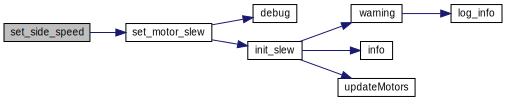
\includegraphics[width=350pt]{drive_8h_a8df41fd50094c065eedc81fc5e6595d1_cgraph}
\end{center}
\end{figure}
Here is the caller graph for this function\+:\nopagebreak
\begin{figure}[H]
\begin{center}
\leavevmode
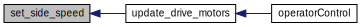
\includegraphics[width=350pt]{drive_8h_a8df41fd50094c065eedc81fc5e6595d1_icgraph}
\end{center}
\end{figure}
\mbox{\Hypertarget{drive_8h_a53d6e35d53ec3e0b1b1c489d8203f204}\label{drive_8h_a53d6e35d53ec3e0b1b1c489d8203f204}} 
\index{drive.\+h@{drive.\+h}!set\+Thresh@{set\+Thresh}}
\index{set\+Thresh@{set\+Thresh}!drive.\+h@{drive.\+h}}
\subsubsection{\texorpdfstring{set\+Thresh()}{setThresh()}}
{\footnotesize\ttfamily void set\+Thresh (\begin{DoxyParamCaption}\item[{int}]{t }\end{DoxyParamCaption})}



Sets the deadzone threshhold on the drive. 

\begin{DoxyAuthor}{Author}
Chris Jerrett 
\end{DoxyAuthor}


Definition at line 17 of file drive.\+c.



References thresh.


\begin{DoxyCode}
17                      \{
18   \hyperlink{drive_8c_a6cf8bf160a02413bc3d5d18b0294b581}{thresh} = t;
19 \}
\end{DoxyCode}
\mbox{\Hypertarget{drive_8h_a8224a4626a934d30ed587671b7004bf8}\label{drive_8h_a8224a4626a934d30ed587671b7004bf8}} 
\index{drive.\+h@{drive.\+h}!update\+\_\+drive\+\_\+motors@{update\+\_\+drive\+\_\+motors}}
\index{update\+\_\+drive\+\_\+motors@{update\+\_\+drive\+\_\+motors}!drive.\+h@{drive.\+h}}
\subsubsection{\texorpdfstring{update\+\_\+drive\+\_\+motors()}{update\_drive\_motors()}}
{\footnotesize\ttfamily void update\+\_\+drive\+\_\+motors (\begin{DoxyParamCaption}{ }\end{DoxyParamCaption})}



Updates the drive motors during teleop. 

\begin{DoxyAuthor}{Author}
Christian Desimone 
\end{DoxyAuthor}
\begin{DoxyDate}{Date}
9/5/17 
\end{DoxyDate}


Definition at line 21 of file drive.\+c.



References get\+\_\+mode(), joystick\+Get\+Analog(), L\+E\+FT, M\+A\+S\+T\+ER, P\+A\+R\+T\+N\+ER, P\+A\+R\+T\+N\+E\+R\+\_\+\+C\+O\+N\+T\+R\+O\+L\+L\+E\+R\+\_\+\+M\+O\+DE, R\+I\+G\+HT, set\+\_\+side\+\_\+speed(), thresh, cord\+::x, and cord\+::y.



Referenced by operator\+Control().


\begin{DoxyCode}
21                           \{
22 
23   \textcolor{keywordtype}{int} \hyperlink{structcord_a2eef9b681474b679cf87b0c20eced2cd}{x} = 0;
24   \textcolor{keywordtype}{int} \hyperlink{structcord_a4e7d289c55cfe511532e53a81dc19215}{y} = 0;
25   \textcolor{keywordflow}{if}(\hyperlink{partner_8h_aacc86d07e59d3b919f5c5eae2ce5d404}{get\_mode}() == \hyperlink{partner_8h_afb2b5bca5ceab5f6efd8bac14a568324a60c19a56177d369da54f4e3d942c7df7}{PARTNER\_CONTROLLER\_MODE}) \{
26     x = (\hyperlink{_a_p_i_8h_ad56fcec15d1a48deb8780bb0fc38be4d}{joystickGetAnalog}(\hyperlink{controller_8h_a136e64cf351535da81cacb6a546cade6}{PARTNER}, 3));
27     y = (\hyperlink{_a_p_i_8h_ad56fcec15d1a48deb8780bb0fc38be4d}{joystickGetAnalog}(\hyperlink{controller_8h_a136e64cf351535da81cacb6a546cade6}{PARTNER}, 1));
28   \} \textcolor{keywordflow}{else} \{
29     x = -(\hyperlink{_a_p_i_8h_ad56fcec15d1a48deb8780bb0fc38be4d}{joystickGetAnalog}(\hyperlink{controller_8h_a3fa2d3bf1901157f734a584d47b25d8b}{MASTER}, 3));
30     y = (\hyperlink{_a_p_i_8h_ad56fcec15d1a48deb8780bb0fc38be4d}{joystickGetAnalog}(\hyperlink{controller_8h_a3fa2d3bf1901157f734a584d47b25d8b}{MASTER}, 1));
31   \}
32 
33   \textcolor{comment}{//x = joystickExp(x);}
34   \textcolor{comment}{//y = joystickExp(y);}
35   \textcolor{keywordflow}{if}(x < thresh && x > -\hyperlink{drive_8c_a6cf8bf160a02413bc3d5d18b0294b581}{thresh})\{
36     x = 0;
37   \}
38   \textcolor{keywordflow}{if}(y < thresh && y > -\hyperlink{drive_8c_a6cf8bf160a02413bc3d5d18b0294b581}{thresh})\{
39     y = 0;
40   \}
41 
42   \textcolor{keywordtype}{int} r = (x + \hyperlink{structcord_a4e7d289c55cfe511532e53a81dc19215}{y});
43   \textcolor{keywordtype}{int} l = -(x - \hyperlink{structcord_a4e7d289c55cfe511532e53a81dc19215}{y});
44 
45   \hyperlink{drive_8c_a8df41fd50094c065eedc81fc5e6595d1}{set\_side\_speed}(\hyperlink{drive_8h_afc015eff6557e84151d2e53b94375445adb45120aafd37a973140edee24708065}{LEFT}, l);
46   \hyperlink{drive_8c_a8df41fd50094c065eedc81fc5e6595d1}{set\_side\_speed}(\hyperlink{drive_8h_afc015eff6557e84151d2e53b94375445aec8379af7490bb9eaaf579cf17876f38}{RIGHT}, -r);
47 
48 \}
\end{DoxyCode}
Here is the call graph for this function\+:\nopagebreak
\begin{figure}[H]
\begin{center}
\leavevmode
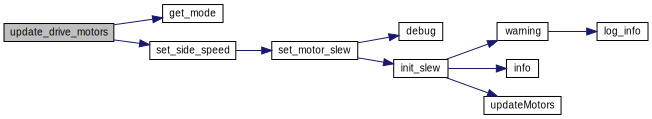
\includegraphics[width=350pt]{drive_8h_a8224a4626a934d30ed587671b7004bf8_cgraph}
\end{center}
\end{figure}
Here is the caller graph for this function\+:\nopagebreak
\begin{figure}[H]
\begin{center}
\leavevmode
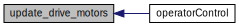
\includegraphics[width=311pt]{drive_8h_a8224a4626a934d30ed587671b7004bf8_icgraph}
\end{center}
\end{figure}

\subsection{drive.\+h}
\label{drive_8h_source}\index{include/drive.\+h@{include/drive.\+h}}

\begin{DoxyCode}
00001 
00008 \textcolor{preprocessor}{#ifndef \_DRIVE\_H\_}
00009 \textcolor{preprocessor}{#define \_DRIVE\_H\_}
00010 
00011 \textcolor{preprocessor}{#include <API.h>}
00012 \textcolor{preprocessor}{#include "partner.h"}
00013 
00018 \textcolor{preprocessor}{#define THRESHOLD 10}
00019 
00026 \textcolor{keyword}{typedef} \textcolor{keyword}{enum} side\{
00027   LEFT,
00028   BOTH,
00029   RIGHT
00030 \} side_t;
00031 
00038 \textcolor{keywordtype}{void} set_side_speed(side_t side, \textcolor{keywordtype}{int} speed);
00039 
00044 \textcolor{keywordtype}{void} setThresh(\textcolor{keywordtype}{int} t);
00045 
00051 \textcolor{keywordtype}{void} update_drive_motors();
00052 
00053 \textcolor{preprocessor}{#endif}
\end{DoxyCode}

\hypertarget{encoders_8h}{}\section{include/encoders.h File Reference}
\label{encoders_8h}\index{include/encoders.\+h@{include/encoders.\+h}}


wrapper around encoder functions  


{\ttfamily \#include $<$A\+P\+I.\+h$>$}\newline
\subsection*{Macros}
\begin{DoxyCompactItemize}
\item 
\#define \hyperlink{encoders_8h_a87db35d2735ef045f57d446b3bfe8d48}{I\+M\+E\+\_\+\+N\+U\+M\+B\+ER}~0
\begin{DoxyCompactList}\small\item\em The number of I\+M\+Es. This number is compared against the number detect in init\+\_\+encoders. \end{DoxyCompactList}\end{DoxyCompactItemize}
\subsection*{Functions}
\begin{DoxyCompactItemize}
\item 
int \hyperlink{encoders_8h_aed261dd4dae33a48c42f2e363c84760f}{get\+\_\+encoder\+\_\+ticks} (unsigned char address)
\begin{DoxyCompactList}\small\item\em Gets the encoder ticks since last reset. \end{DoxyCompactList}\item 
int \hyperlink{encoders_8h_a8e6b77703c5cf18e00709b052fb4bf22}{get\+\_\+encoder\+\_\+velocity} (unsigned char address)
\begin{DoxyCompactList}\small\item\em Gets the encoder reads. \end{DoxyCompactList}\item 
bool \hyperlink{encoders_8h_aa6ec1ca17e907babd52803ecba451cd3}{init\+\_\+encoders} ()
\begin{DoxyCompactList}\small\item\em Initializes all motor encoders. \end{DoxyCompactList}\end{DoxyCompactItemize}


\subsection{Detailed Description}
wrapper around encoder functions 

\begin{DoxyAuthor}{Author}
Chris Jerrett 
\end{DoxyAuthor}
\begin{DoxyDate}{Date}
9/9/2017 
\end{DoxyDate}


\subsection{Macro Definition Documentation}
\mbox{\Hypertarget{encoders_8h_a87db35d2735ef045f57d446b3bfe8d48}\label{encoders_8h_a87db35d2735ef045f57d446b3bfe8d48}} 
\index{encoders.\+h@{encoders.\+h}!I\+M\+E\+\_\+\+N\+U\+M\+B\+ER@{I\+M\+E\+\_\+\+N\+U\+M\+B\+ER}}
\index{I\+M\+E\+\_\+\+N\+U\+M\+B\+ER@{I\+M\+E\+\_\+\+N\+U\+M\+B\+ER}!encoders.\+h@{encoders.\+h}}
\subsubsection{\texorpdfstring{I\+M\+E\+\_\+\+N\+U\+M\+B\+ER}{IME\_NUMBER}}
{\footnotesize\ttfamily \#define I\+M\+E\+\_\+\+N\+U\+M\+B\+ER~0}



The number of I\+M\+Es. This number is compared against the number detect in init\+\_\+encoders. 

\begin{DoxySeeAlso}{See also}
\hyperlink{encoders_8h_aa6ec1ca17e907babd52803ecba451cd3}{init\+\_\+encoders()} 
\end{DoxySeeAlso}
\begin{DoxyAuthor}{Author}
Chris Jerrett 
\end{DoxyAuthor}
\begin{DoxyDate}{Date}
9/9/2017 
\end{DoxyDate}
\begin{DoxySeeAlso}{See also}
\hyperlink{encoders_8h_a87db35d2735ef045f57d446b3bfe8d48}{I\+M\+E\+\_\+\+N\+U\+M\+B\+ER} 
\end{DoxySeeAlso}


Definition at line 21 of file encoders.\+h.



Referenced by init\+\_\+encoders().



\subsection{Function Documentation}
\mbox{\Hypertarget{encoders_8h_aed261dd4dae33a48c42f2e363c84760f}\label{encoders_8h_aed261dd4dae33a48c42f2e363c84760f}} 
\index{encoders.\+h@{encoders.\+h}!get\+\_\+encoder\+\_\+ticks@{get\+\_\+encoder\+\_\+ticks}}
\index{get\+\_\+encoder\+\_\+ticks@{get\+\_\+encoder\+\_\+ticks}!encoders.\+h@{encoders.\+h}}
\subsubsection{\texorpdfstring{get\+\_\+encoder\+\_\+ticks()}{get\_encoder\_ticks()}}
{\footnotesize\ttfamily int get\+\_\+encoder\+\_\+ticks (\begin{DoxyParamCaption}\item[{unsigned char}]{address }\end{DoxyParamCaption})}



Gets the encoder ticks since last reset. 

\begin{DoxyAuthor}{Author}
Chris Jerrett 
\end{DoxyAuthor}
\begin{DoxyDate}{Date}
9/15/2017 
\end{DoxyDate}


Definition at line 12 of file encoders.\+c.


\begin{DoxyCode}
12                                              \{
13   \textcolor{keywordtype}{int} i = 0;
14   imeGet(address, &i);
15   \textcolor{keywordflow}{return} i;
16 \}
\end{DoxyCode}
\mbox{\Hypertarget{encoders_8h_a8e6b77703c5cf18e00709b052fb4bf22}\label{encoders_8h_a8e6b77703c5cf18e00709b052fb4bf22}} 
\index{encoders.\+h@{encoders.\+h}!get\+\_\+encoder\+\_\+velocity@{get\+\_\+encoder\+\_\+velocity}}
\index{get\+\_\+encoder\+\_\+velocity@{get\+\_\+encoder\+\_\+velocity}!encoders.\+h@{encoders.\+h}}
\subsubsection{\texorpdfstring{get\+\_\+encoder\+\_\+velocity()}{get\_encoder\_velocity()}}
{\footnotesize\ttfamily int get\+\_\+encoder\+\_\+velocity (\begin{DoxyParamCaption}\item[{unsigned char}]{address }\end{DoxyParamCaption})}



Gets the encoder reads. 

\begin{DoxyAuthor}{Author}
Chris Jerrett 
\end{DoxyAuthor}
\begin{DoxyDate}{Date}
9/15/2017 
\end{DoxyDate}


Definition at line 18 of file encoders.\+c.


\begin{DoxyCode}
18                                                 \{
19   \textcolor{keywordtype}{int} i = 0;
20   imeGetVelocity(address, &i);
21   \textcolor{keywordflow}{return} i;
22 \}
\end{DoxyCode}
\mbox{\Hypertarget{encoders_8h_aa6ec1ca17e907babd52803ecba451cd3}\label{encoders_8h_aa6ec1ca17e907babd52803ecba451cd3}} 
\index{encoders.\+h@{encoders.\+h}!init\+\_\+encoders@{init\+\_\+encoders}}
\index{init\+\_\+encoders@{init\+\_\+encoders}!encoders.\+h@{encoders.\+h}}
\subsubsection{\texorpdfstring{init\+\_\+encoders()}{init\_encoders()}}
{\footnotesize\ttfamily bool init\+\_\+encoders (\begin{DoxyParamCaption}{ }\end{DoxyParamCaption})}



Initializes all motor encoders. 

\begin{DoxyAuthor}{Author}
Chris Jerrett 
\end{DoxyAuthor}
\begin{DoxyDate}{Date}
9/9/2017 
\end{DoxyDate}
\begin{DoxySeeAlso}{See also}
\hyperlink{encoders_8h_a87db35d2735ef045f57d446b3bfe8d48}{I\+M\+E\+\_\+\+N\+U\+M\+B\+ER} 
\end{DoxySeeAlso}


Definition at line 4 of file encoders.\+c.



References I\+M\+E\+\_\+\+N\+U\+M\+B\+ER.



Referenced by initialize().


\begin{DoxyCode}
4                      \{
5 \textcolor{preprocessor}{  #ifdef IME\_NUMBER}
6   \textcolor{keywordflow}{return} imeInitializeAll() == \hyperlink{encoders_8h_a87db35d2735ef045f57d446b3bfe8d48}{IME\_NUMBER};
7 \textcolor{preprocessor}{  #else}
8   \textcolor{keywordflow}{return} imeInitializeAll();
9 \textcolor{preprocessor}{  #endif}
10 \}
\end{DoxyCode}

\subsection{encoders.\+h}
\label{encoders_8h_source}\index{include/encoders.\+h@{include/encoders.\+h}}

\begin{DoxyCode}
00001 
00007 \textcolor{preprocessor}{#ifndef \_ENCODERS\_H\_}
00008 \textcolor{preprocessor}{#define \_ENCODERS\_H\_}
00009 
00010 \textcolor{preprocessor}{#include <API.h>}
00011 
00020 \textcolor{preprocessor}{#define IME\_NUMBER 6}
00021 
00028 \textcolor{keywordtype}{bool} init_encoders();
00029 
00035 \textcolor{keywordtype}{int} get_encoder_ticks(\textcolor{keywordtype}{unsigned} \textcolor{keywordtype}{char} address);
00036 
00042 \textcolor{keywordtype}{int} get_encoder_velocity(\textcolor{keywordtype}{unsigned} \textcolor{keywordtype}{char} address);
00043 
00044 \textcolor{preprocessor}{#endif}
\end{DoxyCode}

\subsection{include/lcd.h File Reference}
\label{lcd_8h}\index{include/lcd.\+h@{include/lcd.\+h}}


L\+CD wrapper functions and macros.  


\subsubsection*{Data Structures}
\begin{DoxyCompactItemize}
\item 
struct \textbf{ lcd\+\_\+buttons}
\begin{DoxyCompactList}\small\item\em represents the state of the lcd buttons \end{DoxyCompactList}\end{DoxyCompactItemize}
\subsubsection*{Enumerations}
\begin{DoxyCompactItemize}
\item 
enum \textbf{ button\+\_\+state} \{ \textbf{ R\+E\+L\+E\+A\+S\+ED} = false, 
\textbf{ P\+R\+E\+S\+S\+ED} = true
 \}\begin{DoxyCompactList}\small\item\em Represents the state of a button. \end{DoxyCompactList}
\end{DoxyCompactItemize}
\subsubsection*{Functions}
\begin{DoxyCompactItemize}
\item 
void \textbf{ init\+\_\+main\+\_\+lcd} (F\+I\+LE $\ast$lcd)
\begin{DoxyCompactList}\small\item\em Initializes the lcd screen. \end{DoxyCompactList}\item 
void \textbf{ lcd\+\_\+clear} ()
\begin{DoxyCompactList}\small\item\em Clears the lcd. \end{DoxyCompactList}\item 
\textbf{ lcd\+\_\+buttons} \textbf{ lcd\+\_\+get\+\_\+pressed\+\_\+buttons} ()
\begin{DoxyCompactList}\small\item\em Returns the pressed buttons. \end{DoxyCompactList}\item 
void \textbf{ lcd\+\_\+print} (unsigned int \textbf{ line}, const char $\ast$str)
\begin{DoxyCompactList}\small\item\em prints a string to a line on the lcd \end{DoxyCompactList}\item 
void \textbf{ lcd\+\_\+printf} (unsigned int \textbf{ line}, const char $\ast$format\+\_\+str,...)
\begin{DoxyCompactList}\small\item\em prints a formated string to a line on the lcd. \end{DoxyCompactList}\item 
void \textbf{ lcd\+\_\+set\+\_\+backlight} (bool \textbf{ state})
\begin{DoxyCompactList}\small\item\em sets the backlight of the lcd \end{DoxyCompactList}\item 
void \textbf{ promt\+\_\+confirmation} (const char $\ast$confirm\+\_\+text)
\begin{DoxyCompactList}\small\item\em Prompts the user to confirm a string. \end{DoxyCompactList}\end{DoxyCompactItemize}


\subsubsection{Detailed Description}
L\+CD wrapper functions and macros. 

\begin{DoxyAuthor}{Author}
Chris Jerrett 
\end{DoxyAuthor}
\begin{DoxyDate}{Date}
9/9/2017 
\end{DoxyDate}


Definition in file \textbf{ lcd.\+h}.



\subsubsection{Enumeration Type Documentation}
\mbox{\label{lcd_8h_a0bbab92f5605e16a4162b6c5ccc2c29b}} 
\index{lcd.\+h@{lcd.\+h}!button\+\_\+state@{button\+\_\+state}}
\index{button\+\_\+state@{button\+\_\+state}!lcd.\+h@{lcd.\+h}}
\paragraph{button\+\_\+state}
{\footnotesize\ttfamily enum \textbf{ button\+\_\+state}}



Represents the state of a button. 

A button can be pressed of R\+E\+L\+E\+A\+S\+ED. Release is false which is also 0. P\+R\+E\+S\+S\+ED is true or 1.

\begin{DoxyAuthor}{Author}
Chris Jerrett 
\end{DoxyAuthor}
\begin{DoxyDate}{Date}
9/9/2017 
\end{DoxyDate}
\begin{DoxyEnumFields}{Enumerator}
\raisebox{\heightof{T}}[0pt][0pt]{\index{R\+E\+L\+E\+A\+S\+ED@{R\+E\+L\+E\+A\+S\+ED}!lcd.\+h@{lcd.\+h}}\index{lcd.\+h@{lcd.\+h}!R\+E\+L\+E\+A\+S\+ED@{R\+E\+L\+E\+A\+S\+ED}}}\mbox{\label{lcd_8h_a0bbab92f5605e16a4162b6c5ccc2c29baa38d18fe73a7fc82c112b6917d0b5cd0}} 
R\+E\+L\+E\+A\+S\+ED&A released button. \\
\hline

\raisebox{\heightof{T}}[0pt][0pt]{\index{P\+R\+E\+S\+S\+ED@{P\+R\+E\+S\+S\+ED}!lcd.\+h@{lcd.\+h}}\index{lcd.\+h@{lcd.\+h}!P\+R\+E\+S\+S\+ED@{P\+R\+E\+S\+S\+ED}}}\mbox{\label{lcd_8h_a0bbab92f5605e16a4162b6c5ccc2c29ba5ef9a100ac8b4b8d6dec477c377b7901}} 
P\+R\+E\+S\+S\+ED&A pressed button. \\
\hline

\end{DoxyEnumFields}


Definition at line \textbf{ 36} of file \textbf{ lcd.\+h}.


\begin{DoxyCode}
00036              \{
00038   RELEASED = \textcolor{keyword}{false},
00040   PRESSED = \textcolor{keyword}{true},
00041 \} button_state;
\end{DoxyCode}


\subsubsection{Function Documentation}
\mbox{\label{lcd_8h_a93b26f37d6b1687ad54c90feedfd29ca}} 
\index{lcd.\+h@{lcd.\+h}!init\+\_\+main\+\_\+lcd@{init\+\_\+main\+\_\+lcd}}
\index{init\+\_\+main\+\_\+lcd@{init\+\_\+main\+\_\+lcd}!lcd.\+h@{lcd.\+h}}
\paragraph{init\+\_\+main\+\_\+lcd()}
{\footnotesize\ttfamily void init\+\_\+main\+\_\+lcd (\begin{DoxyParamCaption}\item[{F\+I\+LE $\ast$}]{lcd }\end{DoxyParamCaption})}



Initializes the lcd screen. 

Also will initialize the lcd\+\_\+port var. Must be called before any lcd function can be called. 
\begin{DoxyParams}{Parameters}
{\em lcd} & the urart port of the lcd screen \\
\hline
\end{DoxyParams}
\begin{DoxySeeAlso}{See also}
uart1 

uart2 
\end{DoxySeeAlso}
\begin{DoxyAuthor}{Author}
Chris Jerrett 
\end{DoxyAuthor}
\begin{DoxyDate}{Date}
9/9/2017 
\end{DoxyDate}


Definition at line \textbf{ 62} of file \textbf{ lcd.\+c}.



References \textbf{ lcd\+\_\+clear()}, \textbf{ lcd\+\_\+port}, and \textbf{ lcd\+Init()}.



Referenced by \textbf{ initialize()}.


\begin{DoxyCode}
00062                               \{
00063   lcd_port = lcd;
00064   lcdInit(lcd);
00065   lcd_clear();
00066 \}
\end{DoxyCode}
Here is the call graph for this function\+:
\nopagebreak
\begin{figure}[H]
\begin{center}
\leavevmode
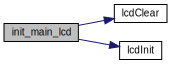
\includegraphics[width=350pt]{lcd_8h_a93b26f37d6b1687ad54c90feedfd29ca_cgraph}
\end{center}
\end{figure}
Here is the caller graph for this function\+:
\nopagebreak
\begin{figure}[H]
\begin{center}
\leavevmode
\includegraphics[width=242pt]{lcd_8h_a93b26f37d6b1687ad54c90feedfd29ca_icgraph}
\end{center}
\end{figure}
\mbox{\label{lcd_8h_a35c08b1fa742e650f4873939707b893b}} 
\index{lcd.\+h@{lcd.\+h}!lcd\+\_\+clear@{lcd\+\_\+clear}}
\index{lcd\+\_\+clear@{lcd\+\_\+clear}!lcd.\+h@{lcd.\+h}}
\paragraph{lcd\+\_\+clear()}
{\footnotesize\ttfamily void lcd\+\_\+clear (\begin{DoxyParamCaption}{ }\end{DoxyParamCaption})}



Clears the lcd. 

\begin{DoxyAuthor}{Author}
Chris Jerrett 
\end{DoxyAuthor}
\begin{DoxyDate}{Date}
9/9/2017 
\end{DoxyDate}


Definition at line \textbf{ 47} of file \textbf{ lcd.\+c}.



References \textbf{ lcd\+\_\+assert()}, \textbf{ lcd\+\_\+port}, and \textbf{ lcd\+Clear()}.



Referenced by \textbf{ display\+\_\+menu()}, and \textbf{ init\+\_\+main\+\_\+lcd()}.


\begin{DoxyCode}
00047                  \{
00048   lcd_assert();
00049   lcdClear(lcd_port);
00050 \}
\end{DoxyCode}
Here is the call graph for this function\+:
\nopagebreak
\begin{figure}[H]
\begin{center}
\leavevmode
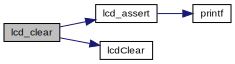
\includegraphics[width=308pt]{lcd_8h_a35c08b1fa742e650f4873939707b893b_cgraph}
\end{center}
\end{figure}
Here is the caller graph for this function\+:
\nopagebreak
\begin{figure}[H]
\begin{center}
\leavevmode
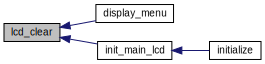
\includegraphics[width=337pt]{lcd_8h_a35c08b1fa742e650f4873939707b893b_icgraph}
\end{center}
\end{figure}
\mbox{\label{lcd_8h_ac7b3225ccc82fcbe067ba9da934f010d}} 
\index{lcd.\+h@{lcd.\+h}!lcd\+\_\+get\+\_\+pressed\+\_\+buttons@{lcd\+\_\+get\+\_\+pressed\+\_\+buttons}}
\index{lcd\+\_\+get\+\_\+pressed\+\_\+buttons@{lcd\+\_\+get\+\_\+pressed\+\_\+buttons}!lcd.\+h@{lcd.\+h}}
\paragraph{lcd\+\_\+get\+\_\+pressed\+\_\+buttons()}
{\footnotesize\ttfamily \textbf{ lcd\+\_\+buttons} lcd\+\_\+get\+\_\+pressed\+\_\+buttons (\begin{DoxyParamCaption}{ }\end{DoxyParamCaption})}



Returns the pressed buttons. 

\begin{DoxyReturn}{Returns}
a struct containing the states of all three buttons. 
\end{DoxyReturn}
\begin{DoxyAuthor}{Author}
Chris Jerrett 
\end{DoxyAuthor}
\begin{DoxyDate}{Date}
9/9/2017 
\end{DoxyDate}
\begin{DoxySeeAlso}{See also}
\doxyref{lcd\+\_\+buttons}{p.}{structlcd__buttons} 
\end{DoxySeeAlso}


Definition at line \textbf{ 28} of file \textbf{ lcd.\+c}.



References \textbf{ lcd\+\_\+assert()}, \textbf{ lcd\+\_\+port}, \textbf{ lcd\+Read\+Buttons()}, \textbf{ lcd\+\_\+buttons\+::left}, \textbf{ lcd\+\_\+buttons\+::middle}, \textbf{ P\+R\+E\+S\+S\+ED}, \textbf{ R\+E\+L\+E\+A\+S\+ED}, and \textbf{ lcd\+\_\+buttons\+::right}.



Referenced by \textbf{ display\+\_\+menu()}, and \textbf{ promt\+\_\+confirmation()}.


\begin{DoxyCode}
00028                                       \{
00029   lcd_assert();
00030   \textcolor{keywordtype}{unsigned} \textcolor{keywordtype}{int} btn\_binary = lcdReadButtons(lcd_port);
00031   \textcolor{keywordtype}{bool} left = btn\_binary & 0x1;   \textcolor{comment}{// 0001}
00032   \textcolor{keywordtype}{bool} middle = btn\_binary & 0x2; \textcolor{comment}{// 0010}
00033   \textcolor{keywordtype}{bool} right = btn\_binary & 0x4;  \textcolor{comment}{// 0100}
00034   lcd_buttons btns;
00035   btns.left = left ? PRESSED : RELEASED;
00036   btns.middle = middle ? PRESSED : RELEASED;
00037   btns.right = right ? PRESSED : RELEASED;
00038 
00039   \textcolor{keywordflow}{return} btns;
00040 \}
\end{DoxyCode}
Here is the call graph for this function\+:
\nopagebreak
\begin{figure}[H]
\begin{center}
\leavevmode
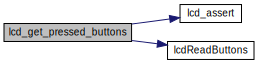
\includegraphics[width=350pt]{lcd_8h_ac7b3225ccc82fcbe067ba9da934f010d_cgraph}
\end{center}
\end{figure}
Here is the caller graph for this function\+:
\nopagebreak
\begin{figure}[H]
\begin{center}
\leavevmode
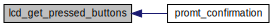
\includegraphics[width=345pt]{lcd_8h_ac7b3225ccc82fcbe067ba9da934f010d_icgraph}
\end{center}
\end{figure}
\mbox{\label{lcd_8h_adabd3f7cdda45119604b488caf22bba8}} 
\index{lcd.\+h@{lcd.\+h}!lcd\+\_\+print@{lcd\+\_\+print}}
\index{lcd\+\_\+print@{lcd\+\_\+print}!lcd.\+h@{lcd.\+h}}
\paragraph{lcd\+\_\+print()}
{\footnotesize\ttfamily void lcd\+\_\+print (\begin{DoxyParamCaption}\item[{unsigned int}]{line,  }\item[{const char $\ast$}]{str }\end{DoxyParamCaption})}



prints a string to a line on the lcd 


\begin{DoxyParams}{Parameters}
{\em line} & the line to print on \\
\hline
{\em str} & string to print \\
\hline
\end{DoxyParams}
\begin{DoxyAuthor}{Author}
Chris Jerrett 
\end{DoxyAuthor}
\begin{DoxyDate}{Date}
9/9/2017 
\end{DoxyDate}


Definition at line \textbf{ 75} of file \textbf{ lcd.\+c}.



References \textbf{ lcd\+\_\+assert()}, \textbf{ lcd\+\_\+port}, and \textbf{ lcd\+Set\+Text()}.



Referenced by \textbf{ display\+\_\+menu()}, and \textbf{ promt\+\_\+confirmation()}.


\begin{DoxyCode}
00075                                                    \{
00076   lcd_assert();
00077   lcdSetText(lcd_port, line, str);
00078 \}
\end{DoxyCode}
Here is the call graph for this function\+:
\nopagebreak
\begin{figure}[H]
\begin{center}
\leavevmode
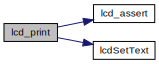
\includegraphics[width=306pt]{lcd_8h_adabd3f7cdda45119604b488caf22bba8_cgraph}
\end{center}
\end{figure}
Here is the caller graph for this function\+:
\nopagebreak
\begin{figure}[H]
\begin{center}
\leavevmode
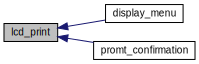
\includegraphics[width=271pt]{lcd_8h_adabd3f7cdda45119604b488caf22bba8_icgraph}
\end{center}
\end{figure}
\mbox{\label{lcd_8h_aa0d4ca88701dfecf98796e2028482b69}} 
\index{lcd.\+h@{lcd.\+h}!lcd\+\_\+printf@{lcd\+\_\+printf}}
\index{lcd\+\_\+printf@{lcd\+\_\+printf}!lcd.\+h@{lcd.\+h}}
\paragraph{lcd\+\_\+printf()}
{\footnotesize\ttfamily void lcd\+\_\+printf (\begin{DoxyParamCaption}\item[{unsigned int}]{line,  }\item[{const char $\ast$}]{format\+\_\+str,  }\item[{}]{... }\end{DoxyParamCaption})}



prints a formated string to a line on the lcd. 

Smilar to printf 
\begin{DoxyParams}{Parameters}
{\em line} & the line to print on \\
\hline
{\em format\+\_\+str} & format string string to print \\
\hline
\end{DoxyParams}
\begin{DoxyAuthor}{Author}
Chris Jerrett 
\end{DoxyAuthor}
\begin{DoxyDate}{Date}
9/9/2017 
\end{DoxyDate}


Definition at line \textbf{ 87} of file \textbf{ lcd.\+c}.



References \textbf{ lcd\+\_\+assert()}, \textbf{ lcd\+\_\+port}, and \textbf{ lcd\+Print()}.


\begin{DoxyCode}
00087                                                                 \{
00088   lcd_assert();
00089   lcdPrint(lcd_port, line, format\_str);
00090 \}
\end{DoxyCode}
Here is the call graph for this function\+:
\nopagebreak
\begin{figure}[H]
\begin{center}
\leavevmode
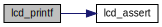
\includegraphics[width=308pt]{lcd_8h_aa0d4ca88701dfecf98796e2028482b69_cgraph}
\end{center}
\end{figure}
\mbox{\label{lcd_8h_a245902a4d48a6d9bd1ab308bf9b7e6b5}} 
\index{lcd.\+h@{lcd.\+h}!lcd\+\_\+set\+\_\+backlight@{lcd\+\_\+set\+\_\+backlight}}
\index{lcd\+\_\+set\+\_\+backlight@{lcd\+\_\+set\+\_\+backlight}!lcd.\+h@{lcd.\+h}}
\paragraph{lcd\+\_\+set\+\_\+backlight()}
{\footnotesize\ttfamily void lcd\+\_\+set\+\_\+backlight (\begin{DoxyParamCaption}\item[{bool}]{state }\end{DoxyParamCaption})}



sets the backlight of the lcd 


\begin{DoxyParams}{Parameters}
{\em state} & a boolean representing the state of the backlight. true = on, false = off. \\
\hline
\end{DoxyParams}
\begin{DoxyAuthor}{Author}
Chris Jerrett 
\end{DoxyAuthor}
\begin{DoxyDate}{Date}
9/9/2017 
\end{DoxyDate}


Definition at line \textbf{ 99} of file \textbf{ lcd.\+c}.



References \textbf{ lcd\+\_\+assert()}, \textbf{ lcd\+\_\+port}, and \textbf{ lcd\+Set\+Backlight()}.


\begin{DoxyCode}
00099                                    \{
00100   lcd_assert();
00101   lcdSetBacklight(lcd_port, state);
00102 \}
\end{DoxyCode}
Here is the call graph for this function\+:
\nopagebreak
\begin{figure}[H]
\begin{center}
\leavevmode
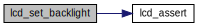
\includegraphics[width=350pt]{lcd_8h_a245902a4d48a6d9bd1ab308bf9b7e6b5_cgraph}
\end{center}
\end{figure}
\mbox{\label{lcd_8h_a99f4683e1990edf624ab216bf327cba4}} 
\index{lcd.\+h@{lcd.\+h}!promt\+\_\+confirmation@{promt\+\_\+confirmation}}
\index{promt\+\_\+confirmation@{promt\+\_\+confirmation}!lcd.\+h@{lcd.\+h}}
\paragraph{promt\+\_\+confirmation()}
{\footnotesize\ttfamily void promt\+\_\+confirmation (\begin{DoxyParamCaption}\item[{const char $\ast$}]{confirm\+\_\+text }\end{DoxyParamCaption})}



Prompts the user to confirm a string. 

User must press middle button to confirm. Function is not thread safe and will stall a thread.


\begin{DoxyParams}{Parameters}
{\em confirm\+\_\+text} & the text for the user to confirm. \\
\hline
\end{DoxyParams}
\begin{DoxyAuthor}{Author}
Chris Jerrett 
\end{DoxyAuthor}
\begin{DoxyDate}{Date}
9/9/2017 
\end{DoxyDate}


Definition at line \textbf{ 113} of file \textbf{ lcd.\+c}.



References \textbf{ delay()}, \textbf{ lcd\+\_\+assert()}, \textbf{ lcd\+\_\+get\+\_\+pressed\+\_\+buttons()}, \textbf{ lcd\+\_\+print()}, and \textbf{ P\+R\+E\+S\+S\+ED}.


\begin{DoxyCode}
00113                                                   \{
00114   lcd_assert();
00115   lcd_print(1, confirm\_text);
00116   \textcolor{keywordflow}{while} (lcd_get_pressed_buttons().middle != PRESSED) \{
00117     delay(200);
00118   \}
00119 \}
\end{DoxyCode}
Here is the call graph for this function\+:
\nopagebreak
\begin{figure}[H]
\begin{center}
\leavevmode
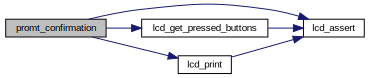
\includegraphics[width=350pt]{lcd_8h_a99f4683e1990edf624ab216bf327cba4_cgraph}
\end{center}
\end{figure}

\subsection{lcd.\+h}
\label{lcd_8h_source}\index{include/lcd.\+h@{include/lcd.\+h}}

\begin{DoxyCode}
00001 
00008 \textcolor{preprocessor}{#ifndef \_LCD\_H\_}
00009 \textcolor{preprocessor}{#define \_LCD\_H\_}
00010 
00011 \textcolor{preprocessor}{#include <API.h>}
00012 
00018 \textcolor{preprocessor}{#define TOP\_ROW 1}
00019 
00025 \textcolor{preprocessor}{#define BOTTOM\_ROW 2}
00026 
00036 \textcolor{keyword}{typedef} \textcolor{keyword}{enum} \{
00038   RELEASED = \textcolor{keyword}{false},
00040   PRESSED = \textcolor{keyword}{true},
00041 \} button_state;
00042 
00048 \textcolor{keyword}{typedef} \textcolor{keyword}{struct }\{
00049   button_state left;
00050   button_state middle;
00051   button_state right;
00052 \} lcd_buttons;
00053 
00054 
00062 lcd_buttons lcd_get_pressed_buttons();
00063 
00069 \textcolor{keywordtype}{void} lcd_clear();
00070 
00080 \textcolor{keywordtype}{void} init_main_lcd(FILE *lcd);
00081 
00089 \textcolor{keywordtype}{void} lcd_print(\textcolor{keywordtype}{unsigned} \textcolor{keywordtype}{int} line, \textcolor{keyword}{const} \textcolor{keywordtype}{char} *str);
00090 
00098 \textcolor{keywordtype}{void} lcd_printf(\textcolor{keywordtype}{unsigned} \textcolor{keywordtype}{int} line, \textcolor{keyword}{const} \textcolor{keywordtype}{char} *format\_str, ...);
00099 
00106 \textcolor{keywordtype}{void} lcd_set_backlight(\textcolor{keywordtype}{bool} state);
00107 
00117 \textcolor{keywordtype}{void} promt_confirmation(\textcolor{keyword}{const} \textcolor{keywordtype}{char} *confirm\_text);
00118 
00119 \textcolor{preprocessor}{#endif}
\end{DoxyCode}

\subsection{include/lifter.h File Reference}
\label{lifter_8h}\index{include/lifter.\+h@{include/lifter.\+h}}


Declarations and macros for controlling and manipulating the lifter.  


\subsubsection*{Functions}
\begin{DoxyCompactItemize}
\item 
void \textbf{ autostack\+\_\+routine} (void $\ast$param)
\begin{DoxyCompactList}\small\item\em Autostacks a cone once picked up. \end{DoxyCompactList}\item 
double \textbf{ get\+Lifter\+Height} ()
\begin{DoxyCompactList}\small\item\em Gets the height of the lifter in inches. \end{DoxyCompactList}\item 
int \textbf{ get\+Lifter\+Ticks} ()
\begin{DoxyCompactList}\small\item\em Gets the value of the lifter pot. \end{DoxyCompactList}\item 
void \textbf{ interrupt\+\_\+auto\+\_\+stack} (void $\ast$param)
\begin{DoxyCompactList}\small\item\em Stpos an autostack in case of an error. \end{DoxyCompactList}\item 
float \textbf{ lifter\+Potentiometer\+To\+Degree} (int x)
\begin{DoxyCompactList}\small\item\em height of the lifter in degrees from 0 height \end{DoxyCompactList}\item 
void \textbf{ lower\+\_\+main\+\_\+lifter} ()
\begin{DoxyCompactList}\small\item\em Lowers the main lifter. \end{DoxyCompactList}\item 
void \textbf{ lower\+\_\+secondary\+\_\+lifter} ()
\begin{DoxyCompactList}\small\item\em Lowers the secondary lifter. \end{DoxyCompactList}\item 
void \textbf{ raise\+\_\+main\+\_\+lifter} ()
\begin{DoxyCompactList}\small\item\em Raises the main lifter. \end{DoxyCompactList}\item 
void \textbf{ raise\+\_\+secondary\+\_\+lifter} ()
\begin{DoxyCompactList}\small\item\em Raises the main lifter. \end{DoxyCompactList}\item 
void \textbf{ set\+\_\+lifter\+\_\+pos} (int pos)
\begin{DoxyCompactList}\small\item\em Sets the lifter positions to the given value. \end{DoxyCompactList}\item 
void \textbf{ set\+\_\+main\+\_\+lifter\+\_\+motors} (const int v)
\begin{DoxyCompactList}\small\item\em Sets the main lifter motors to the given value. \end{DoxyCompactList}\item 
void \textbf{ set\+\_\+secondary\+\_\+lifter\+\_\+motors} (const int v)
\begin{DoxyCompactList}\small\item\em Sets the secondary lifter motors to the given value. \end{DoxyCompactList}\item 
void \textbf{ update\+\_\+lifter} ()
\begin{DoxyCompactList}\small\item\em Updates the lifter in teleop. \end{DoxyCompactList}\end{DoxyCompactItemize}


\subsubsection{Detailed Description}
Declarations and macros for controlling and manipulating the lifter. 

\begin{DoxyAuthor}{Author}
Chris Jerrett, Christian Desimone 
\end{DoxyAuthor}
\begin{DoxyDate}{Date}
8/27/2017 
\end{DoxyDate}


Definition in file \textbf{ lifter.\+h}.



\subsubsection{Function Documentation}
\mbox{\label{lifter_8h_a8a64fa88b389b39c236c5c57a7fb5c67}} 
\index{lifter.\+h@{lifter.\+h}!autostack\+\_\+routine@{autostack\+\_\+routine}}
\index{autostack\+\_\+routine@{autostack\+\_\+routine}!lifter.\+h@{lifter.\+h}}
\paragraph{autostack\+\_\+routine()}
{\footnotesize\ttfamily void autostack\+\_\+routine (\begin{DoxyParamCaption}\item[{void $\ast$}]{param }\end{DoxyParamCaption})}



Autostacks a cone once picked up. 


\begin{DoxyParams}{Parameters}
{\em param} & ignored parameter \\
\hline
\end{DoxyParams}


Definition at line \textbf{ 20} of file \textbf{ lifter.\+c}.



References \textbf{ analog\+Read()}, \textbf{ delay()}, \textbf{ info()}, \textbf{ lifter\+\_\+autostack\+\_\+routine\+\_\+interupt}, \textbf{ lifter\+\_\+autostack\+\_\+running}, \textbf{ lifter\+\_\+ultrasonic}, \textbf{ printf()}, \textbf{ quit\+\_\+auto\+\_\+static()}, \textbf{ raise\+\_\+secondary\+\_\+lifter()}, \textbf{ set\+\_\+claw\+\_\+motor()}, \textbf{ set\+\_\+main\+\_\+lifter\+\_\+motors()}, \textbf{ set\+\_\+secondary\+\_\+lifter\+\_\+motors()}, and \textbf{ ultrasonic\+Get()}.



Referenced by \textbf{ operator\+Control()}.


\begin{DoxyCode}
00020                                     \{
00021   lifter_autostack_routine_interupt = \textcolor{keyword}{false};
00022   lifter_autostack_running = \textcolor{keyword}{true};
00023   raise_secondary_lifter();
00024   \textcolor{keywordflow}{while} (analogRead(SECONDARY\_LIFTER\_POT\_PORT) < 1600) \{
00025     set_secondary_lifter_motors(MIN\_SPEED);
00026     \textcolor{keywordflow}{if} (lifter_autostack_routine_interupt) \{
00027       quit_auto_static();
00028       \textcolor{keywordflow}{return};
00029     \}
00030     delay(50);
00031     info(\textcolor{stringliteral}{"1"});
00032   \}
00033   set_secondary_lifter_motors(0);
00034   \textcolor{keywordtype}{bool} lifted = \textcolor{keyword}{false};
00035   \textcolor{keywordtype}{int} val = ultrasonicGet(lifter_ultrasonic);
00036   printf(\textcolor{stringliteral}{"%d\(\backslash\)n"}, val);
00037   \textcolor{keywordflow}{while} (val < 10 && val != ULTRA\_BAD\_RESPONSE) \{
00038     \textcolor{keywordflow}{if} (lifter_autostack_routine_interupt) \{
00039       quit_auto_static();
00040       \textcolor{keywordflow}{return};
00041     \}
00042     set_main_lifter_motors(MAX\_SPEED);
00043     info(\textcolor{stringliteral}{"2"});
00044     lifted = \textcolor{keyword}{true};
00045     delay(50);
00046     val = ultrasonicGet(lifter_ultrasonic);
00047     printf(\textcolor{stringliteral}{"%d\(\backslash\)n"}, val);
00048   \}
00049   \textcolor{keywordflow}{if} (lifter_autostack_routine_interupt) \{
00050     quit_auto_static();
00051     \textcolor{keywordflow}{return};
00052   \}
00053   delay(200);
00054   \textcolor{keywordflow}{if} (lifted)
00055     delay(50);
00056   \textcolor{keywordflow}{if} (lifter_autostack_routine_interupt) \{
00057     quit_auto_static();
00058     \textcolor{keywordflow}{return};
00059   \}
00060   set_main_lifter_motors(0);
00061   set_secondary_lifter_motors(0);
00062 
00063   \textcolor{keywordflow}{while} (analogRead(SECONDARY\_LIFTER\_POT\_PORT) < 3000) \{
00064     \textcolor{keywordflow}{if} (lifter_autostack_routine_interupt) \{
00065       quit_auto_static();
00066       \textcolor{keywordflow}{return};
00067     \}
00068     set_secondary_lifter_motors(MIN\_SPEED);
00069     delay(50);
00070     info(\textcolor{stringliteral}{"3"});
00071   \}
00072 
00073   set_main_lifter_motors(MIN\_SPEED / 1.333);
00074 
00075   \textcolor{keywordflow}{while} (val > 10) \{
00076     \textcolor{keywordflow}{if} (lifter_autostack_routine_interupt) \{
00077       quit_auto_static();
00078       \textcolor{keywordflow}{return};
00079     \}
00080     info(\textcolor{stringliteral}{"2"});
00081     lifted = \textcolor{keyword}{true};
00082     delay(30);
00083     val = ultrasonicGet(lifter_ultrasonic);
00084     printf(\textcolor{stringliteral}{"%d\(\backslash\)n"}, val);
00085   \}
00086 
00087   set_main_lifter_motors(0);
00088 
00089   set_claw_motor(MIN\_CLAW\_SPEED);
00090   \textcolor{keywordflow}{if} (lifter_autostack_routine_interupt) \{
00091     quit_auto_static();
00092     \textcolor{keywordflow}{return};
00093   \}
00094   delay(500);
00095   \textcolor{keywordflow}{if} (lifter_autostack_routine_interupt) \{
00096     quit_auto_static();
00097     \textcolor{keywordflow}{return};
00098   \}
00099   set_main_lifter_motors(MAX\_SPEED);
00100   \textcolor{keywordflow}{if} (lifter_autostack_routine_interupt) \{
00101     quit_auto_static();
00102     \textcolor{keywordflow}{return};
00103   \}
00104   delay(300);
00105 
00106   set_main_lifter_motors(MIN\_SPEED);
00107   set_claw_motor(0);
00108   set_secondary_lifter_motors(0);
00109 
00110   lifter_autostack_running = \textcolor{keyword}{false};
00111 \}
\end{DoxyCode}
Here is the call graph for this function\+:
\nopagebreak
\begin{figure}[H]
\begin{center}
\leavevmode
\includegraphics[width=350pt]{lifter_8h_a8a64fa88b389b39c236c5c57a7fb5c67_cgraph}
\end{center}
\end{figure}
Here is the caller graph for this function\+:
\nopagebreak
\begin{figure}[H]
\begin{center}
\leavevmode
\includegraphics[width=296pt]{lifter_8h_a8a64fa88b389b39c236c5c57a7fb5c67_icgraph}
\end{center}
\end{figure}
\mbox{\label{lifter_8h_a2719740958fd8a5926f88f6194e820e3}} 
\index{lifter.\+h@{lifter.\+h}!get\+Lifter\+Height@{get\+Lifter\+Height}}
\index{get\+Lifter\+Height@{get\+Lifter\+Height}!lifter.\+h@{lifter.\+h}}
\paragraph{get\+Lifter\+Height()}
{\footnotesize\ttfamily double get\+Lifter\+Height (\begin{DoxyParamCaption}{ }\end{DoxyParamCaption})}



Gets the height of the lifter in inches. 

\begin{DoxyReturn}{Returns}
the height of the lifter. 
\end{DoxyReturn}
\begin{DoxyAuthor}{Author}
Chris Jerrett 
\end{DoxyAuthor}
\begin{DoxyDate}{Date}
9/17/2017 
\end{DoxyDate}


Definition at line \textbf{ 306} of file \textbf{ lifter.\+c}.



References \textbf{ get\+Lifter\+Ticks()}.


\begin{DoxyCode}
00306                          \{
00307   \textcolor{keywordtype}{unsigned} \textcolor{keywordtype}{int} ticks = getLifterTicks();
00308   \textcolor{keywordflow}{return} (-2 * pow(10, (-9 * ticks)) + 6 * (pow(10, (-6 * ticks * ticks))) +
00309           0.0198 * ticks + 2.3033);
00310 \}
\end{DoxyCode}
Here is the call graph for this function\+:
\nopagebreak
\begin{figure}[H]
\begin{center}
\leavevmode
\includegraphics[width=350pt]{lifter_8h_a2719740958fd8a5926f88f6194e820e3_cgraph}
\end{center}
\end{figure}
\mbox{\label{lifter_8h_acdf909159b0406c48099843f2306be78}} 
\index{lifter.\+h@{lifter.\+h}!get\+Lifter\+Ticks@{get\+Lifter\+Ticks}}
\index{get\+Lifter\+Ticks@{get\+Lifter\+Ticks}!lifter.\+h@{lifter.\+h}}
\paragraph{get\+Lifter\+Ticks()}
{\footnotesize\ttfamily int get\+Lifter\+Ticks (\begin{DoxyParamCaption}{ }\end{DoxyParamCaption})}



Gets the value of the lifter pot. 

\begin{DoxyReturn}{Returns}
the value of the pot. 
\end{DoxyReturn}
\begin{DoxyAuthor}{Author}
Chris Jerrett 
\end{DoxyAuthor}
\begin{DoxyDate}{Date}
9/9/2017 
\end{DoxyDate}


Definition at line \textbf{ 297} of file \textbf{ lifter.\+c}.



References \textbf{ analog\+Read()}.



Referenced by \textbf{ get\+Lifter\+Height()}.


\begin{DoxyCode}
00297 \{ \textcolor{keywordflow}{return} analogRead(LIFTER); \}
\end{DoxyCode}
Here is the call graph for this function\+:
\nopagebreak
\begin{figure}[H]
\begin{center}
\leavevmode
\includegraphics[width=261pt]{lifter_8h_acdf909159b0406c48099843f2306be78_cgraph}
\end{center}
\end{figure}
Here is the caller graph for this function\+:
\nopagebreak
\begin{figure}[H]
\begin{center}
\leavevmode
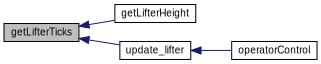
\includegraphics[width=272pt]{lifter_8h_acdf909159b0406c48099843f2306be78_icgraph}
\end{center}
\end{figure}
\mbox{\label{lifter_8h_a3738d33dc870f98243a93bddd855b43e}} 
\index{lifter.\+h@{lifter.\+h}!interrupt\+\_\+auto\+\_\+stack@{interrupt\+\_\+auto\+\_\+stack}}
\index{interrupt\+\_\+auto\+\_\+stack@{interrupt\+\_\+auto\+\_\+stack}!lifter.\+h@{lifter.\+h}}
\paragraph{interrupt\+\_\+auto\+\_\+stack()}
{\footnotesize\ttfamily void interrupt\+\_\+auto\+\_\+stack (\begin{DoxyParamCaption}\item[{void $\ast$}]{param }\end{DoxyParamCaption})}



Stpos an autostack in case of an error. 


\begin{DoxyParams}{Parameters}
{\em param} & ignore parameter \\
\hline
\end{DoxyParams}


Definition at line \textbf{ 8} of file \textbf{ lifter.\+c}.



References \textbf{ info()}, and \textbf{ lifter\+\_\+autostack\+\_\+routine\+\_\+interupt}.



Referenced by \textbf{ operator\+Control()}.


\begin{DoxyCode}
00008                                        \{
00009   info(\textcolor{stringliteral}{"int"});
00010   lifter_autostack_routine_interupt = \textcolor{keyword}{true};
00011 \}
\end{DoxyCode}
Here is the call graph for this function\+:
\nopagebreak
\begin{figure}[H]
\begin{center}
\leavevmode
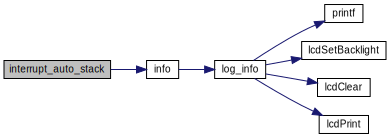
\includegraphics[width=350pt]{lifter_8h_a3738d33dc870f98243a93bddd855b43e_cgraph}
\end{center}
\end{figure}
Here is the caller graph for this function\+:
\nopagebreak
\begin{figure}[H]
\begin{center}
\leavevmode
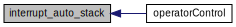
\includegraphics[width=308pt]{lifter_8h_a3738d33dc870f98243a93bddd855b43e_icgraph}
\end{center}
\end{figure}
\mbox{\label{lifter_8h_ab0460888f3213e5510bd25ae1e152a75}} 
\index{lifter.\+h@{lifter.\+h}!lifter\+Potentiometer\+To\+Degree@{lifter\+Potentiometer\+To\+Degree}}
\index{lifter\+Potentiometer\+To\+Degree@{lifter\+Potentiometer\+To\+Degree}!lifter.\+h@{lifter.\+h}}
\paragraph{lifter\+Potentiometer\+To\+Degree()}
{\footnotesize\ttfamily float lifter\+Potentiometer\+To\+Degree (\begin{DoxyParamCaption}\item[{int}]{x }\end{DoxyParamCaption})}



height of the lifter in degrees from 0 height 


\begin{DoxyParams}{Parameters}
{\em x} & the pot value \\
\hline
\end{DoxyParams}
\begin{DoxyReturn}{Returns}
the positions in degrees 
\end{DoxyReturn}
\begin{DoxyAuthor}{Author}
Chris Jerrett 
\end{DoxyAuthor}
\begin{DoxyDate}{Date}
10/13/2017 
\end{DoxyDate}


Definition at line \textbf{ 286} of file \textbf{ lifter.\+c}.


\begin{DoxyCode}
00286                                          \{
00287   \textcolor{keywordflow}{return} (x - INIT\_ROTATION) / TICK\_MAX * DEG\_MAX;
00288 \}
\end{DoxyCode}
\mbox{\label{lifter_8h_ad36c37086a91046af4e6f619618b7719}} 
\index{lifter.\+h@{lifter.\+h}!lower\+\_\+main\+\_\+lifter@{lower\+\_\+main\+\_\+lifter}}
\index{lower\+\_\+main\+\_\+lifter@{lower\+\_\+main\+\_\+lifter}!lifter.\+h@{lifter.\+h}}
\paragraph{lower\+\_\+main\+\_\+lifter()}
{\footnotesize\ttfamily void lower\+\_\+main\+\_\+lifter (\begin{DoxyParamCaption}{ }\end{DoxyParamCaption})}



Lowers the main lifter. 

\begin{DoxyAuthor}{Author}
Christian De\+Simone 
\end{DoxyAuthor}
\begin{DoxyDate}{Date}
9/12/2017 
\end{DoxyDate}


Definition at line \textbf{ 160} of file \textbf{ lifter.\+c}.



References \textbf{ set\+\_\+main\+\_\+lifter\+\_\+motors()}.


\begin{DoxyCode}
00160 \{ set_main_lifter_motors(MAX\_SPEED); \}
\end{DoxyCode}
Here is the call graph for this function\+:
\nopagebreak
\begin{figure}[H]
\begin{center}
\leavevmode
\includegraphics[width=350pt]{lifter_8h_ad36c37086a91046af4e6f619618b7719_cgraph}
\end{center}
\end{figure}
\mbox{\label{lifter_8h_af76abbd394bf206ab56fa237d776f2b3}} 
\index{lifter.\+h@{lifter.\+h}!lower\+\_\+secondary\+\_\+lifter@{lower\+\_\+secondary\+\_\+lifter}}
\index{lower\+\_\+secondary\+\_\+lifter@{lower\+\_\+secondary\+\_\+lifter}!lifter.\+h@{lifter.\+h}}
\paragraph{lower\+\_\+secondary\+\_\+lifter()}
{\footnotesize\ttfamily void lower\+\_\+secondary\+\_\+lifter (\begin{DoxyParamCaption}{ }\end{DoxyParamCaption})}



Lowers the secondary lifter. 

\begin{DoxyAuthor}{Author}
Christian De\+Simone 
\end{DoxyAuthor}
\begin{DoxyDate}{Date}
9/12/2017 
\end{DoxyDate}


Definition at line \textbf{ 176} of file \textbf{ lifter.\+c}.



References \textbf{ set\+\_\+secondary\+\_\+lifter\+\_\+motors()}.


\begin{DoxyCode}
00176 \{ set_secondary_lifter_motors(MAX\_SPEED); \}
\end{DoxyCode}
Here is the call graph for this function\+:
\nopagebreak
\begin{figure}[H]
\begin{center}
\leavevmode
\includegraphics[width=350pt]{lifter_8h_af76abbd394bf206ab56fa237d776f2b3_cgraph}
\end{center}
\end{figure}
\mbox{\label{lifter_8h_a2e2bd38b5b8b52378f3510368bf8aa0a}} 
\index{lifter.\+h@{lifter.\+h}!raise\+\_\+main\+\_\+lifter@{raise\+\_\+main\+\_\+lifter}}
\index{raise\+\_\+main\+\_\+lifter@{raise\+\_\+main\+\_\+lifter}!lifter.\+h@{lifter.\+h}}
\paragraph{raise\+\_\+main\+\_\+lifter()}
{\footnotesize\ttfamily void raise\+\_\+main\+\_\+lifter (\begin{DoxyParamCaption}{ }\end{DoxyParamCaption})}



Raises the main lifter. 

\begin{DoxyAuthor}{Author}
Christian De\+Simone 
\end{DoxyAuthor}
\begin{DoxyDate}{Date}
9/12/2017 
\end{DoxyDate}


Definition at line \textbf{ 152} of file \textbf{ lifter.\+c}.



References \textbf{ set\+\_\+main\+\_\+lifter\+\_\+motors()}.


\begin{DoxyCode}
00152 \{ set_main_lifter_motors(MAX\_SPEED); \}
\end{DoxyCode}
Here is the call graph for this function\+:
\nopagebreak
\begin{figure}[H]
\begin{center}
\leavevmode
\includegraphics[width=350pt]{lifter_8h_a2e2bd38b5b8b52378f3510368bf8aa0a_cgraph}
\end{center}
\end{figure}
\mbox{\label{lifter_8h_a786f679ea48bb8c80e00fbac9a69911b}} 
\index{lifter.\+h@{lifter.\+h}!raise\+\_\+secondary\+\_\+lifter@{raise\+\_\+secondary\+\_\+lifter}}
\index{raise\+\_\+secondary\+\_\+lifter@{raise\+\_\+secondary\+\_\+lifter}!lifter.\+h@{lifter.\+h}}
\paragraph{raise\+\_\+secondary\+\_\+lifter()}
{\footnotesize\ttfamily void raise\+\_\+secondary\+\_\+lifter (\begin{DoxyParamCaption}{ }\end{DoxyParamCaption})}



Raises the main lifter. 

\begin{DoxyAuthor}{Author}
Christian De\+Simone 
\end{DoxyAuthor}
\begin{DoxyDate}{Date}
9/12/2017 
\end{DoxyDate}


Definition at line \textbf{ 168} of file \textbf{ lifter.\+c}.



References \textbf{ set\+\_\+secondary\+\_\+lifter\+\_\+motors()}.



Referenced by \textbf{ autostack\+\_\+routine()}.


\begin{DoxyCode}
00168 \{ set_secondary_lifter_motors(MIN\_SPEED / 1.5); \}
\end{DoxyCode}
Here is the call graph for this function\+:
\nopagebreak
\begin{figure}[H]
\begin{center}
\leavevmode
\includegraphics[width=350pt]{lifter_8h_a786f679ea48bb8c80e00fbac9a69911b_cgraph}
\end{center}
\end{figure}
Here is the caller graph for this function\+:
\nopagebreak
\begin{figure}[H]
\begin{center}
\leavevmode
\includegraphics[width=350pt]{lifter_8h_a786f679ea48bb8c80e00fbac9a69911b_icgraph}
\end{center}
\end{figure}
\mbox{\label{lifter_8h_abddc7cb502e12fa277b627c90a45efb1}} 
\index{lifter.\+h@{lifter.\+h}!set\+\_\+lifter\+\_\+pos@{set\+\_\+lifter\+\_\+pos}}
\index{set\+\_\+lifter\+\_\+pos@{set\+\_\+lifter\+\_\+pos}!lifter.\+h@{lifter.\+h}}
\paragraph{set\+\_\+lifter\+\_\+pos()}
{\footnotesize\ttfamily void set\+\_\+lifter\+\_\+pos (\begin{DoxyParamCaption}\item[{int}]{pos }\end{DoxyParamCaption})}



Sets the lifter positions to the given value. 


\begin{DoxyParams}{Parameters}
{\em pos} & The height in inches \\
\hline
\end{DoxyParams}
\begin{DoxyAuthor}{Author}
Chris Jerrett 
\end{DoxyAuthor}
\begin{DoxyDate}{Date}
9/12/2017 
\end{DoxyDate}


Definition at line \textbf{ 144} of file \textbf{ lifter.\+c}.


\begin{DoxyCode}
00144 \{\}
\end{DoxyCode}
\mbox{\label{lifter_8h_ad00a195af30f246924d6e1a30095b882}} 
\index{lifter.\+h@{lifter.\+h}!set\+\_\+main\+\_\+lifter\+\_\+motors@{set\+\_\+main\+\_\+lifter\+\_\+motors}}
\index{set\+\_\+main\+\_\+lifter\+\_\+motors@{set\+\_\+main\+\_\+lifter\+\_\+motors}!lifter.\+h@{lifter.\+h}}
\paragraph{set\+\_\+main\+\_\+lifter\+\_\+motors()}
{\footnotesize\ttfamily void set\+\_\+main\+\_\+lifter\+\_\+motors (\begin{DoxyParamCaption}\item[{const int}]{v }\end{DoxyParamCaption})}



Sets the main lifter motors to the given value. 


\begin{DoxyParams}{Parameters}
{\em v} & value for the lifter motor. Between -\/128 -\/ 127, any values outside are clamped. \\
\hline
\end{DoxyParams}
\begin{DoxyAuthor}{Author}
Chris Jerrett 
\end{DoxyAuthor}
\begin{DoxyDate}{Date}
9/9/2017 
\end{DoxyDate}


Definition at line \textbf{ 133} of file \textbf{ lifter.\+c}.



References \textbf{ set\+\_\+motor\+\_\+slew()}.



Referenced by \textbf{ auton\+\_\+rasie\+\_\+main\+\_\+lifter()}, \textbf{ autostack\+\_\+routine()}, \textbf{ lower\+\_\+main\+\_\+lifter()}, \textbf{ main\+\_\+lifter\+\_\+update()}, \textbf{ quit\+\_\+auto\+\_\+static()}, and \textbf{ raise\+\_\+main\+\_\+lifter()}.


\begin{DoxyCode}
00133                                          \{
00134   set_motor_slew(MOTOR\_MAIN\_LIFTER, v);
00135 \}
\end{DoxyCode}
Here is the call graph for this function\+:
\nopagebreak
\begin{figure}[H]
\begin{center}
\leavevmode
\includegraphics[width=350pt]{lifter_8h_ad00a195af30f246924d6e1a30095b882_cgraph}
\end{center}
\end{figure}
Here is the caller graph for this function\+:
\nopagebreak
\begin{figure}[H]
\begin{center}
\leavevmode
\includegraphics[width=350pt]{lifter_8h_ad00a195af30f246924d6e1a30095b882_icgraph}
\end{center}
\end{figure}
\mbox{\label{lifter_8h_a78640d547d9361951a92d0bc00939536}} 
\index{lifter.\+h@{lifter.\+h}!set\+\_\+secondary\+\_\+lifter\+\_\+motors@{set\+\_\+secondary\+\_\+lifter\+\_\+motors}}
\index{set\+\_\+secondary\+\_\+lifter\+\_\+motors@{set\+\_\+secondary\+\_\+lifter\+\_\+motors}!lifter.\+h@{lifter.\+h}}
\paragraph{set\+\_\+secondary\+\_\+lifter\+\_\+motors()}
{\footnotesize\ttfamily void set\+\_\+secondary\+\_\+lifter\+\_\+motors (\begin{DoxyParamCaption}\item[{const int}]{v }\end{DoxyParamCaption})}



Sets the secondary lifter motors to the given value. 


\begin{DoxyParams}{Parameters}
{\em v} & value for the lifter motor. Between -\/128 -\/ 127, any values outside are clamped. \\
\hline
\end{DoxyParams}
\begin{DoxyAuthor}{Author}
Chris Jerrett 
\end{DoxyAuthor}
\begin{DoxyDate}{Date}
1/6/2018 
\end{DoxyDate}


Definition at line \textbf{ 121} of file \textbf{ lifter.\+c}.



References \textbf{ set\+\_\+motor\+\_\+immediate()}.



Referenced by \textbf{ auton\+\_\+raise\+\_\+sec\+\_\+lifter\+\_\+max()}, \textbf{ autonomous()}, \textbf{ autostack\+\_\+routine()}, \textbf{ deploy\+\_\+seoncdary\+\_\+lifter()}, \textbf{ lower\+\_\+secondary\+\_\+lifter()}, \textbf{ quit\+\_\+auto\+\_\+static()}, \textbf{ raise\+\_\+secondary\+\_\+lifter()}, and \textbf{ secondary\+\_\+lifter\+\_\+update()}.


\begin{DoxyCode}
00121                                               \{
00122   set_motor_immediate(MOTOR\_SECONDARY\_LIFTER, v);
00123 \}
\end{DoxyCode}
Here is the call graph for this function\+:
\nopagebreak
\begin{figure}[H]
\begin{center}
\leavevmode
\includegraphics[width=350pt]{lifter_8h_a78640d547d9361951a92d0bc00939536_cgraph}
\end{center}
\end{figure}
Here is the caller graph for this function\+:
\nopagebreak
\begin{figure}[H]
\begin{center}
\leavevmode
\includegraphics[width=350pt]{lifter_8h_a78640d547d9361951a92d0bc00939536_icgraph}
\end{center}
\end{figure}
\mbox{\label{lifter_8h_a59bb7413777ca16aba124aaedf95c79b}} 
\index{lifter.\+h@{lifter.\+h}!update\+\_\+lifter@{update\+\_\+lifter}}
\index{update\+\_\+lifter@{update\+\_\+lifter}!lifter.\+h@{lifter.\+h}}
\paragraph{update\+\_\+lifter()}
{\footnotesize\ttfamily void update\+\_\+lifter (\begin{DoxyParamCaption}{ }\end{DoxyParamCaption})}



Updates the lifter in teleop. 

\begin{DoxyAuthor}{Author}
Chris Jerrett 
\end{DoxyAuthor}
\begin{DoxyDate}{Date}
9/9/2017 
\end{DoxyDate}


Definition at line \textbf{ 272} of file \textbf{ lifter.\+c}.



References \textbf{ analog\+Read()}, \textbf{ main\+\_\+lifter\+\_\+update()}, \textbf{ printf()}, \textbf{ secondary\+\_\+lifter\+\_\+update()}, and \textbf{ secondary\+\_\+override}.



Referenced by \textbf{ operator\+Control()}.


\begin{DoxyCode}
00272                      \{
00273   printf(\textcolor{stringliteral}{"%d \(\backslash\)n"}, analogRead(SECONDARY\_LIFTER\_POT\_PORT));
00274   main_lifter_update();
00275   \textcolor{keywordflow}{if} (!secondary_override)
00276     secondary_lifter_update();
00277 \}
\end{DoxyCode}
Here is the call graph for this function\+:
\nopagebreak
\begin{figure}[H]
\begin{center}
\leavevmode
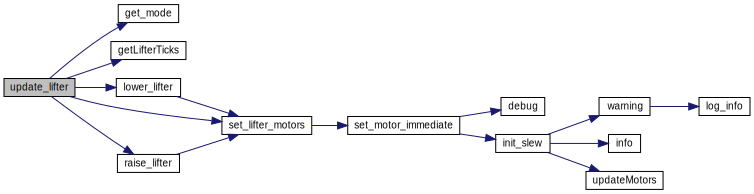
\includegraphics[width=350pt]{lifter_8h_a59bb7413777ca16aba124aaedf95c79b_cgraph}
\end{center}
\end{figure}
Here is the caller graph for this function\+:
\nopagebreak
\begin{figure}[H]
\begin{center}
\leavevmode
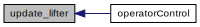
\includegraphics[width=273pt]{lifter_8h_a59bb7413777ca16aba124aaedf95c79b_icgraph}
\end{center}
\end{figure}

\subsection{lifter.\+h}
\label{lifter_8h_source}\index{include/lifter.\+h@{include/lifter.\+h}}

\begin{DoxyCode}
00001 
00007 \textcolor{preprocessor}{#ifndef \_LIFTER\_H\_}
00008 \textcolor{preprocessor}{#define \_LIFTER\_H\_}
00009 
00010 \textcolor{preprocessor}{#include "controller.h"}
00011 \textcolor{preprocessor}{#include "drive.h"}
00012 \textcolor{preprocessor}{#include "motor_ports.h"}
00013 \textcolor{preprocessor}{#include "potentiometer.h"}
00014 \textcolor{preprocessor}{#include "sensors.h"}
00015 \textcolor{preprocessor}{#include "slew.h"}
00016 \textcolor{preprocessor}{#include <API.h>}
00017 
00021 \textcolor{preprocessor}{#define INIT\_ROTATION 680}
00022 
00026 \textcolor{preprocessor}{#define SECONDARY\_LIFTER\_P .05}
00027 
00031 \textcolor{preprocessor}{#define SECONDARY\_LIFTER\_D 0}
00032 
00036 \textcolor{preprocessor}{#define SECONDARY\_LIFTER\_I 0.000}
00037 
00041 \textcolor{preprocessor}{#define MAIN\_LIFTER\_P 0}
00042 
00046 \textcolor{preprocessor}{#define MAIN\_LIFTER\_D 0}
00047 
00051 \textcolor{preprocessor}{#define MAIN\_LIFTER\_I 0.0000001}
00052 
00056 \textcolor{preprocessor}{#define THRESHOLD 10}
00057 
00061 \textcolor{preprocessor}{#define HEIGHT 19.1 - 3.8}
00062 
00066 \textcolor{preprocessor}{#define LIFTER\_UP PARTNER, 6, JOY\_UP}
00067 
00071 \textcolor{preprocessor}{#define LIFTER\_DOWN PARTNER, 6, JOY\_DOWN}
00072 
00076 \textcolor{preprocessor}{#define SECONDARY\_LIFTER\_UP PARTNER, 5, JOY\_UP}
00077 
00081 \textcolor{preprocessor}{#define SECONDARY\_LIFTER\_DOWN PARTNER, 5, JOY\_DOWN}
00082 
00086 \textcolor{preprocessor}{#define LIFTER\_DRIVER\_LOAD MASTER, RIGHT\_BUTTONS, JOY\_RIGHT}
00087 
00091 \textcolor{preprocessor}{#define LIFTER\_UP\_PARTNER PARTNER, 5, JOY\_UP}
00092 
00096 \textcolor{preprocessor}{#define LIFTER\_DOWN\_PARTNER PARTNER, 5, JOY\_DOWN}
00097 
00101 \textcolor{preprocessor}{#define SECONDARY\_LIFTER\_POT\_PORT 2}
00102 
00106 \textcolor{preprocessor}{#define SECONDARY\_LIFTER\_MAX\_HEIGHT 3120}
00107 
00111 \textcolor{preprocessor}{#define SECONDARY\_LIFTER\_MIN\_HEIGHT 2000}
00112 
00116 \textcolor{preprocessor}{#define MAIN\_LIFTER\_POT 1}
00117 
00121 \textcolor{preprocessor}{#define MAIN\_LIFTER\_MIN\_HEIGHT 1700}
00122 
00131 \textcolor{keywordtype}{void} set_secondary_lifter_motors(\textcolor{keyword}{const} \textcolor{keywordtype}{int} v);
00132 
00141 \textcolor{keywordtype}{void} set_main_lifter_motors(\textcolor{keyword}{const} \textcolor{keywordtype}{int} v);
00142 
00150 \textcolor{keywordtype}{void} set_lifter_pos(\textcolor{keywordtype}{int} pos);
00151 
00158 \textcolor{keywordtype}{void} raise_main_lifter();
00159 
00166 \textcolor{keywordtype}{void} lower_main_lifter();
00167 
00174 \textcolor{keywordtype}{void} raise_secondary_lifter();
00175 
00182 \textcolor{keywordtype}{void} lower_secondary_lifter();
00183 
00190 \textcolor{keywordtype}{void} update_lifter();
00191 
00200 \textcolor{keywordtype}{float} lifterPotentiometerToDegree(\textcolor{keywordtype}{int} x);
00201 
00209 \textcolor{keywordtype}{int} getLifterTicks();
00210 
00218 \textcolor{keywordtype}{double} getLifterHeight();
00219 
00224 \textcolor{keywordtype}{void} autostack_routine(\textcolor{keywordtype}{void} *param);
00225 
00230 \textcolor{keywordtype}{void} interrupt_auto_stack(\textcolor{keywordtype}{void} *param);
00231 
00232 \textcolor{preprocessor}{#endif}
\end{DoxyCode}

\subsection{include/localization.h File Reference}
\label{localization_8h}\index{include/localization.\+h@{include/localization.\+h}}


Declarations and macros for determining the location of the robot. [W\+IP].  


{\ttfamily \#include \char`\"{}encoders.\+h\char`\"{}}\newline
{\ttfamily \#include \char`\"{}matrix.\+h\char`\"{}}\newline
{\ttfamily \#include $<$A\+P\+I.\+h$>$}\newline
{\ttfamily \#include $<$math.\+h$>$}\newline
\subsubsection*{Data Structures}
\begin{DoxyCompactItemize}
\item 
struct \textbf{ location}
\end{DoxyCompactItemize}
\subsubsection*{Macros}
\begin{DoxyCompactItemize}
\item 
\#define \textbf{ L\+O\+C\+A\+L\+I\+Z\+A\+T\+I\+O\+N\+\_\+\+U\+P\+D\+A\+T\+E\+\_\+\+F\+R\+E\+Q\+U\+E\+N\+CY}~0.\+500
\end{DoxyCompactItemize}
\subsubsection*{Functions}
\begin{DoxyCompactItemize}
\item 
int \textbf{ calculate\+\_\+encoder\+\_\+angle} ()
\item 
struct \textbf{ location} \textbf{ get\+\_\+position} ()
\begin{DoxyCompactList}\small\item\em Gets the current posituion of the robot. \end{DoxyCompactList}\item 
bool \textbf{ init\+\_\+localization} (const unsigned char gyro1, unsigned short multiplier, int start\+\_\+x, int start\+\_\+y, int start\+\_\+theta)
\begin{DoxyCompactList}\small\item\em Starts the localization process. \end{DoxyCompactList}\item 
void \textbf{ update\+\_\+position} ()
\begin{DoxyCompactList}\small\item\em Updates the position from the localization. \end{DoxyCompactList}\end{DoxyCompactItemize}


\subsubsection{Detailed Description}
Declarations and macros for determining the location of the robot. [W\+IP]. 

\begin{DoxyAuthor}{Author}
Chris Jerrett, Christian Desimone 
\end{DoxyAuthor}
\begin{DoxyDate}{Date}
9/27/2017 
\end{DoxyDate}


Definition in file \textbf{ localization.\+h}.



\subsubsection{Macro Definition Documentation}
\mbox{\label{localization_8h_a4fa0a97f6aafe983a46ffc7188d1fab5}} 
\index{localization.\+h@{localization.\+h}!L\+O\+C\+A\+L\+I\+Z\+A\+T\+I\+O\+N\+\_\+\+U\+P\+D\+A\+T\+E\+\_\+\+F\+R\+E\+Q\+U\+E\+N\+CY@{L\+O\+C\+A\+L\+I\+Z\+A\+T\+I\+O\+N\+\_\+\+U\+P\+D\+A\+T\+E\+\_\+\+F\+R\+E\+Q\+U\+E\+N\+CY}}
\index{L\+O\+C\+A\+L\+I\+Z\+A\+T\+I\+O\+N\+\_\+\+U\+P\+D\+A\+T\+E\+\_\+\+F\+R\+E\+Q\+U\+E\+N\+CY@{L\+O\+C\+A\+L\+I\+Z\+A\+T\+I\+O\+N\+\_\+\+U\+P\+D\+A\+T\+E\+\_\+\+F\+R\+E\+Q\+U\+E\+N\+CY}!localization.\+h@{localization.\+h}}
\paragraph{L\+O\+C\+A\+L\+I\+Z\+A\+T\+I\+O\+N\+\_\+\+U\+P\+D\+A\+T\+E\+\_\+\+F\+R\+E\+Q\+U\+E\+N\+CY}
{\footnotesize\ttfamily \#define L\+O\+C\+A\+L\+I\+Z\+A\+T\+I\+O\+N\+\_\+\+U\+P\+D\+A\+T\+E\+\_\+\+F\+R\+E\+Q\+U\+E\+N\+CY~0.\+500}

How often the localization code updates the position. 

Definition at line \textbf{ 19} of file \textbf{ localization.\+h}.



Referenced by \textbf{ calculate\+\_\+gryo\+\_\+anglular\+\_\+velocity()}, \textbf{ init\+\_\+localization()}, and \textbf{ integrate\+\_\+gyro\+\_\+w()}.



\subsubsection{Function Documentation}
\mbox{\label{localization_8h_a5dd17937f5561711cd12cdefa8d31869}} 
\index{localization.\+h@{localization.\+h}!calculate\+\_\+encoder\+\_\+angle@{calculate\+\_\+encoder\+\_\+angle}}
\index{calculate\+\_\+encoder\+\_\+angle@{calculate\+\_\+encoder\+\_\+angle}!localization.\+h@{localization.\+h}}
\paragraph{calculate\+\_\+encoder\+\_\+angle()}
{\footnotesize\ttfamily int calculate\+\_\+encoder\+\_\+angle (\begin{DoxyParamCaption}{ }\end{DoxyParamCaption})}



Definition at line \textbf{ 101} of file \textbf{ localization.\+c}.



References \textbf{ C\+PR}, \textbf{ get\+\_\+encoder\+\_\+ticks()}, and \textbf{ W\+I\+D\+TH}.



Referenced by \textbf{ autonomous()}.

\mbox{\label{localization_8h_aadbff35bb757f60bc348d4d778f57a2f}} 
\index{localization.\+h@{localization.\+h}!get\+\_\+position@{get\+\_\+position}}
\index{get\+\_\+position@{get\+\_\+position}!localization.\+h@{localization.\+h}}
\paragraph{get\+\_\+position()}
{\footnotesize\ttfamily struct \textbf{ location} get\+\_\+position (\begin{DoxyParamCaption}{ }\end{DoxyParamCaption})}



Gets the current posituion of the robot. 


\begin{DoxyParams}{Parameters}
{\em gyro1} & The first gyro \\
\hline
\end{DoxyParams}
\begin{DoxyReturn}{Returns}
the loacation of the robot as a struct. 
\end{DoxyReturn}


Definition at line \textbf{ 32} of file \textbf{ localization.\+c}.

\mbox{\label{localization_8h_afdd0147de6aa15957e9a125f9cd20578}} 
\index{localization.\+h@{localization.\+h}!init\+\_\+localization@{init\+\_\+localization}}
\index{init\+\_\+localization@{init\+\_\+localization}!localization.\+h@{localization.\+h}}
\paragraph{init\+\_\+localization()}
{\footnotesize\ttfamily bool init\+\_\+localization (\begin{DoxyParamCaption}\item[{const unsigned char}]{gyro1,  }\item[{unsigned short}]{multiplier,  }\item[{int}]{start\+\_\+x,  }\item[{int}]{start\+\_\+y,  }\item[{int}]{start\+\_\+theta }\end{DoxyParamCaption})}



Starts the localization process. 

\begin{DoxyAuthor}{Author}
Chris Jerrett
\end{DoxyAuthor}

\begin{DoxyParams}{Parameters}
{\em gyro1} & The first gyro  The multiplier parameter can tune the gyro to adapt to specific sensors. The default value at this time is 196; higher values will increase the number of degrees reported for a fixed actual rotation, while lower values will decrease the number of degrees reported. If your robot is consistently turning too far, increase the multiplier, and if it is not turning far enough, decrease the multiplier. \\
\hline
\end{DoxyParams}


Definition at line \textbf{ 123} of file \textbf{ localization.\+c}.



References \textbf{ g1}, \textbf{ last\+\_\+call}, \textbf{ localization\+\_\+task}, \textbf{ L\+O\+C\+A\+L\+I\+Z\+A\+T\+I\+O\+N\+\_\+\+U\+P\+D\+A\+T\+E\+\_\+\+F\+R\+E\+Q\+U\+E\+N\+CY}, \textbf{ make\+Matrix()}, and \textbf{ update\+\_\+position()}.

\mbox{\label{localization_8h_afacd5e0b3d5e677df26a4402bbd9ec9e}} 
\index{localization.\+h@{localization.\+h}!update\+\_\+position@{update\+\_\+position}}
\index{update\+\_\+position@{update\+\_\+position}!localization.\+h@{localization.\+h}}
\paragraph{update\+\_\+position()}
{\footnotesize\ttfamily void update\+\_\+position (\begin{DoxyParamCaption}{ }\end{DoxyParamCaption})}



Updates the position from the localization. 

\begin{DoxyAuthor}{Author}
Chris Jerrett 
\end{DoxyAuthor}


Definition at line \textbf{ 39} of file \textbf{ localization.\+c}.



References \textbf{ calculate\+\_\+accelerometer\+\_\+odemetry()}, and \textbf{ last\+\_\+call}.



Referenced by \textbf{ init\+\_\+localization()}.


\subsection{localization.\+h}
\label{localization_8h_source}\index{include/localization.\+h@{include/localization.\+h}}

\begin{DoxyCode}
00001 
00007 \textcolor{preprocessor}{#ifndef \_LOCALIZATION\_H\_}
00008 \textcolor{preprocessor}{#define \_LOCALIZATION\_H\_}
00009 
00010 \textcolor{preprocessor}{#include <API.h>}
00011 \textcolor{preprocessor}{#include "encoders.h"}
00012 \textcolor{preprocessor}{#include <math.h>}
00013 \textcolor{preprocessor}{#include "matrix.h"}
00014 
00018 \textcolor{preprocessor}{#define LOCALIZATION\_UPDATE\_FREQUENCY 0.500}
00019 
00023 \textcolor{keyword}{struct }location \{
00024   \textcolor{keywordtype}{int} x;
00025   \textcolor{keywordtype}{int} y;
00026   \textcolor{keywordtype}{int} theta;
00027 \};
00028 
00040 \textcolor{keywordtype}{bool} init_localization(\textcolor{keyword}{const} \textcolor{keywordtype}{unsigned} \textcolor{keywordtype}{char} gyro1, \textcolor{keywordtype}{unsigned} \textcolor{keywordtype}{short} multiplier, \textcolor{keywordtype}{int} start\_x, \textcolor{keywordtype}{int} start\_y, \textcolor{keywordtype}{int} 
      start\_theta);
00041 
00048 \textcolor{keyword}{struct }location get_position();
00049 
00050 \textcolor{preprocessor}{#endif}
\end{DoxyCode}

\section{include/log.h File Reference}
\label{log_8h}\index{include/log.\+h@{include/log.\+h}}


Contains logging functions.  


{\ttfamily \#include $<$A\+P\+I.\+h$>$}\newline
{\ttfamily \#include \char`\"{}lcd.\+h\char`\"{}}\newline
Include dependency graph for log.\+h\+:
\nopagebreak
\begin{figure}[H]
\begin{center}
\leavevmode
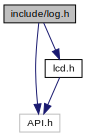
\includegraphics[width=159pt]{log_8h__incl}
\end{center}
\end{figure}
This graph shows which files directly or indirectly include this file\+:
\nopagebreak
\begin{figure}[H]
\begin{center}
\leavevmode
\includegraphics[width=350pt]{log_8h__dep__incl}
\end{center}
\end{figure}
\subsection*{Macros}
\begin{DoxyCompactItemize}
\item 
\#define \textbf{ D\+E\+B\+UG}~4
\begin{DoxyCompactList}\small\item\em logging only info debug. most verbose level \end{DoxyCompactList}\item 
\#define \textbf{ E\+R\+R\+OR}~1
\begin{DoxyCompactList}\small\item\em logging only errors. Also displays error to lcd \end{DoxyCompactList}\item 
\#define \textbf{ I\+N\+FO}~3
\begin{DoxyCompactList}\small\item\em logging only info messages and higher. \end{DoxyCompactList}\item 
\#define \textbf{ N\+O\+NE}~0
\begin{DoxyCompactList}\small\item\em No logging. Should be used in competition to reduce serial communication. \end{DoxyCompactList}\item 
\#define \textbf{ W\+A\+R\+N\+I\+NG}~2
\begin{DoxyCompactList}\small\item\em logs errors and warnings. Also displays error to lcd \end{DoxyCompactList}\end{DoxyCompactItemize}
\subsection*{Functions}
\begin{DoxyCompactItemize}
\item 
void \textbf{ debug} (const char $\ast$debug\+\_\+message)
\begin{DoxyCompactList}\small\item\em prints a info message \end{DoxyCompactList}\item 
void \textbf{ error} (const char $\ast$error\+\_\+message)
\begin{DoxyCompactList}\small\item\em prints a error message and displays on lcd. Only will print and display if log\+\_\+level is greater than N\+O\+NE \end{DoxyCompactList}\item 
void \textbf{ info} (const char $\ast$info\+\_\+message)
\begin{DoxyCompactList}\small\item\em prints a info message \end{DoxyCompactList}\item 
void \textbf{ init\+\_\+error} (bool use\+\_\+lcd, F\+I\+LE $\ast$lcd)
\begin{DoxyCompactList}\small\item\em Initializes the error lcd system Only required if using lcd. \end{DoxyCompactList}\item 
void \textbf{ warning} (const char $\ast$warning\+\_\+message)
\begin{DoxyCompactList}\small\item\em prints a warning message and displays on lcd. Only will print and display if log\+\_\+level is greater than N\+O\+NE \end{DoxyCompactList}\end{DoxyCompactItemize}


\subsection{Detailed Description}
Contains logging functions. 

\begin{DoxyAuthor}{Author}
Chris Jerrett 
\end{DoxyAuthor}
\begin{DoxyDate}{Date}
9/16/2017 
\end{DoxyDate}


Definition in file \textbf{ log.\+h}.



\subsection{Macro Definition Documentation}
\mbox{\label{log_8h_ad72dbcf6d0153db1b8d8a58001feed83}} 
\index{log.\+h@{log.\+h}!D\+E\+B\+UG@{D\+E\+B\+UG}}
\index{D\+E\+B\+UG@{D\+E\+B\+UG}!log.\+h@{log.\+h}}
\subsubsection{D\+E\+B\+UG}
{\footnotesize\ttfamily \#define D\+E\+B\+UG~4}



logging only info debug. most verbose level 

\begin{DoxyAuthor}{Author}
Chris Jerrett 
\end{DoxyAuthor}
\begin{DoxyDate}{Date}
9/10/17 
\end{DoxyDate}


Definition at line \textbf{ 50} of file \textbf{ log.\+h}.

\mbox{\label{log_8h_a8fe83ac76edc595f6b98cd4a4127aed5}} 
\index{log.\+h@{log.\+h}!E\+R\+R\+OR@{E\+R\+R\+OR}}
\index{E\+R\+R\+OR@{E\+R\+R\+OR}!log.\+h@{log.\+h}}
\subsubsection{E\+R\+R\+OR}
{\footnotesize\ttfamily \#define E\+R\+R\+OR~1}



logging only errors. Also displays error to lcd 

\begin{DoxyAuthor}{Author}
Chris Jerrett 
\end{DoxyAuthor}
\begin{DoxyDate}{Date}
9/10/17 
\end{DoxyDate}


Definition at line \textbf{ 27} of file \textbf{ log.\+h}.



Referenced by \textbf{ debug()}, and \textbf{ info()}.

\mbox{\label{log_8h_ae1103fea1e1b3c41ca3322d5389f7162}} 
\index{log.\+h@{log.\+h}!I\+N\+FO@{I\+N\+FO}}
\index{I\+N\+FO@{I\+N\+FO}!log.\+h@{log.\+h}}
\subsubsection{I\+N\+FO}
{\footnotesize\ttfamily \#define I\+N\+FO~3}



logging only info messages and higher. 

\begin{DoxyAuthor}{Author}
Chris Jerrett 
\end{DoxyAuthor}
\begin{DoxyDate}{Date}
9/10/17 
\end{DoxyDate}


Definition at line \textbf{ 42} of file \textbf{ log.\+h}.

\mbox{\label{log_8h_a655c84af1b0034986ff56e12e84f983d}} 
\index{log.\+h@{log.\+h}!N\+O\+NE@{N\+O\+NE}}
\index{N\+O\+NE@{N\+O\+NE}!log.\+h@{log.\+h}}
\subsubsection{N\+O\+NE}
{\footnotesize\ttfamily \#define N\+O\+NE~0}



No logging. Should be used in competition to reduce serial communication. 

\begin{DoxyAuthor}{Author}
Chris Jerrett 
\end{DoxyAuthor}
\begin{DoxyDate}{Date}
9/10/17 
\end{DoxyDate}


Definition at line \textbf{ 19} of file \textbf{ log.\+h}.



Referenced by \textbf{ error()}.

\mbox{\label{log_8h_a5cb439d9f933fde4cf23caa370c030e7}} 
\index{log.\+h@{log.\+h}!W\+A\+R\+N\+I\+NG@{W\+A\+R\+N\+I\+NG}}
\index{W\+A\+R\+N\+I\+NG@{W\+A\+R\+N\+I\+NG}!log.\+h@{log.\+h}}
\subsubsection{W\+A\+R\+N\+I\+NG}
{\footnotesize\ttfamily \#define W\+A\+R\+N\+I\+NG~2}



logs errors and warnings. Also displays error to lcd 

\begin{DoxyAuthor}{Author}
Chris Jerrett 
\end{DoxyAuthor}
\begin{DoxyDate}{Date}
9/10/17 
\end{DoxyDate}


Definition at line \textbf{ 35} of file \textbf{ log.\+h}.



Referenced by \textbf{ warning()}.



\subsection{Function Documentation}
\mbox{\label{log_8h_af3668f40d1ad1b4f3418869ac9a31f34}} 
\index{log.\+h@{log.\+h}!debug@{debug}}
\index{debug@{debug}!log.\+h@{log.\+h}}
\subsubsection{debug()}
{\footnotesize\ttfamily void debug (\begin{DoxyParamCaption}\item[{const char $\ast$}]{debug\+\_\+message }\end{DoxyParamCaption})}



prints a info message 

Only will print and display if log\+\_\+level is greater than info \begin{DoxySeeAlso}{See also}
\doxyref{log\+\_\+level}{p.}{log_8c_a8cf62743dafa288b58bd7c6028ec28e5} 
\end{DoxySeeAlso}

\begin{DoxyParams}{Parameters}
{\em debug\+\_\+message} & the message \\
\hline
\end{DoxyParams}


Definition at line \textbf{ 77} of file \textbf{ log.\+c}.



References \textbf{ E\+R\+R\+OR}, and \textbf{ log\+\_\+level}.



Referenced by \textbf{ set\+\_\+motor\+\_\+immediate()}, and \textbf{ set\+\_\+motor\+\_\+slew()}.


\begin{DoxyCode}
00077                                       \{
00078   \textcolor{keywordflow}{if}(log_level>ERROR) \{
00079     printf(\textcolor{stringliteral}{"[INFO]: %s\(\backslash\)n"}, debug\_message);
00080   \}
00081 \}
\end{DoxyCode}
\mbox{\label{log_8h_a8e5bb8a2a372f5b066ff7af7044584c1}} 
\index{log.\+h@{log.\+h}!error@{error}}
\index{error@{error}!log.\+h@{log.\+h}}
\subsubsection{error()}
{\footnotesize\ttfamily void error (\begin{DoxyParamCaption}\item[{const char $\ast$}]{error\+\_\+message }\end{DoxyParamCaption})}



prints a error message and displays on lcd. Only will print and display if log\+\_\+level is greater than N\+O\+NE 

\begin{DoxySeeAlso}{See also}
\doxyref{log\+\_\+level}{p.}{log_8c_a8cf62743dafa288b58bd7c6028ec28e5} 
\end{DoxySeeAlso}
\begin{DoxyAuthor}{Author}
Chris Jerrett 
\end{DoxyAuthor}
\begin{DoxyDate}{Date}
9/10/17 
\end{DoxyDate}

\begin{DoxyParams}{Parameters}
{\em error\+\_\+message} & the message \\
\hline
\end{DoxyParams}


Definition at line \textbf{ 39} of file \textbf{ log.\+c}.



References \textbf{ log\+\_\+info()}, \textbf{ log\+\_\+level}, and \textbf{ N\+O\+NE}.



Referenced by \textbf{ create\+\_\+menu()}.


\begin{DoxyCode}
00039                                       \{
00040   \textcolor{keywordflow}{if}(log_level>NONE)
00041     log_info(\textcolor{stringliteral}{"ERROR"}, error\_message);
00042 \}
\end{DoxyCode}
\mbox{\label{log_8h_a1606d750e1bb8de9f9e917172bba3382}} 
\index{log.\+h@{log.\+h}!info@{info}}
\index{info@{info}!log.\+h@{log.\+h}}
\subsubsection{info()}
{\footnotesize\ttfamily void info (\begin{DoxyParamCaption}\item[{const char $\ast$}]{info\+\_\+message }\end{DoxyParamCaption})}



prints a info message 

Only will print and display if log\+\_\+level is greater than E\+R\+R\+OR \begin{DoxySeeAlso}{See also}
\doxyref{log\+\_\+level}{p.}{log_8c_a8cf62743dafa288b58bd7c6028ec28e5} 
\end{DoxySeeAlso}

\begin{DoxyParams}{Parameters}
{\em info\+\_\+message} & the message \\
\hline
\end{DoxyParams}


Definition at line \textbf{ 64} of file \textbf{ log.\+c}.



References \textbf{ E\+R\+R\+OR}, \textbf{ log\+\_\+info()}, and \textbf{ log\+\_\+level}.



Referenced by \textbf{ init\+\_\+slew()}, and \textbf{ initialize()}.


\begin{DoxyCode}
00064                                     \{
00065   \textcolor{keywordflow}{if}(log_level>ERROR) \{
00066     log_info(\textcolor{stringliteral}{"INFO"}, info\_message);
00067   \}
00068 \}
\end{DoxyCode}
\mbox{\label{log_8h_a163f389b4f5cf440a807d8fb48aaa006}} 
\index{log.\+h@{log.\+h}!init\+\_\+error@{init\+\_\+error}}
\index{init\+\_\+error@{init\+\_\+error}!log.\+h@{log.\+h}}
\subsubsection{init\+\_\+error()}
{\footnotesize\ttfamily void init\+\_\+error (\begin{DoxyParamCaption}\item[{bool}]{use\+\_\+lcd,  }\item[{F\+I\+LE $\ast$}]{lcd }\end{DoxyParamCaption})}



Initializes the error lcd system Only required if using lcd. 

\begin{DoxyAuthor}{Author}
Chris Jerrett 
\end{DoxyAuthor}
\begin{DoxyDate}{Date}
9/10/17 
\end{DoxyDate}

\begin{DoxyParams}{Parameters}
{\em use\+\_\+lcd} & whether to use the lcd \\
\hline
{\em lcd} & the lcd \\
\hline
\end{DoxyParams}


Definition at line \textbf{ 14} of file \textbf{ log.\+c}.



References \textbf{ log\+\_\+lcd}.



Referenced by \textbf{ initialize()}.


\begin{DoxyCode}
00014                                          \{
00015   \textcolor{keywordflow}{if}(use\_lcd) \{
00016     lcdInit(lcd);
00017     log_lcd = lcd;
00018     lcdClear(log_lcd);
00019     printf(\textcolor{stringliteral}{"LCD Init\(\backslash\)n"});
00020   \}
00021 \}
\end{DoxyCode}
\mbox{\label{log_8h_a0bec2cf5fff7f607bc510b74aba9887c}} 
\index{log.\+h@{log.\+h}!warning@{warning}}
\index{warning@{warning}!log.\+h@{log.\+h}}
\subsubsection{warning()}
{\footnotesize\ttfamily void warning (\begin{DoxyParamCaption}\item[{const char $\ast$}]{warning\+\_\+message }\end{DoxyParamCaption})}



prints a warning message and displays on lcd. Only will print and display if log\+\_\+level is greater than N\+O\+NE 

\begin{DoxySeeAlso}{See also}
\doxyref{log\+\_\+level}{p.}{log_8c_a8cf62743dafa288b58bd7c6028ec28e5} 
\end{DoxySeeAlso}
\begin{DoxyAuthor}{Author}
Chris Jerrett 
\end{DoxyAuthor}
\begin{DoxyDate}{Date}
9/10/17 
\end{DoxyDate}

\begin{DoxyParams}{Parameters}
{\em warning\+\_\+message} & the message \\
\hline
\end{DoxyParams}


Definition at line \textbf{ 52} of file \textbf{ log.\+c}.



References \textbf{ log\+\_\+info()}, \textbf{ log\+\_\+level}, and \textbf{ W\+A\+R\+N\+I\+NG}.



Referenced by \textbf{ init\+\_\+slew()}.


\begin{DoxyCode}
00052                                           \{
00053   \textcolor{keywordflow}{if}(log_level>WARNING)
00054     log_info(\textcolor{stringliteral}{"WARNING"}, warning\_message);
00055 \}
\end{DoxyCode}

\subsection{log.\+h}
\label{log_8h_source}\index{include/log.\+h@{include/log.\+h}}

\begin{DoxyCode}
00001 
00007 \textcolor{preprocessor}{#ifndef \_LOG\_H\_}
00008 \textcolor{preprocessor}{#define \_LOG\_H\_}
00009 
00010 \textcolor{preprocessor}{#include "lcd.h"}
00011 \textcolor{preprocessor}{#include <API.h>}
00012 
00019 \textcolor{preprocessor}{#define NONE 0}
00020 
00027 \textcolor{preprocessor}{#define ERROR 1}
00028 
00035 \textcolor{preprocessor}{#define WARNING 2}
00036 
00042 \textcolor{preprocessor}{#define INFO 3}
00043 
00050 \textcolor{preprocessor}{#define DEBUG 4}
00051 
00060 \textcolor{keywordtype}{void} init_error(\textcolor{keywordtype}{bool} use\_lcd, FILE *lcd);
00061 
00070 \textcolor{keywordtype}{void} error(\textcolor{keyword}{const} \textcolor{keywordtype}{char} *error\_message);
00071 
00080 \textcolor{keywordtype}{void} warning(\textcolor{keyword}{const} \textcolor{keywordtype}{char} *warning\_message);
00081 
00089 \textcolor{keywordtype}{void} info(\textcolor{keyword}{const} \textcolor{keywordtype}{char} *info\_message);
00090 
00098 \textcolor{keywordtype}{void} debug(\textcolor{keyword}{const} \textcolor{keywordtype}{char} *debug\_message);
00099 
00100 \textcolor{preprocessor}{#endif}
\end{DoxyCode}

\subsection{include/main.h File Reference}
\label{main_8h}\index{include/main.\+h@{include/main.\+h}}


Header file for global functions.  


{\ttfamily \#include $<$A\+P\+I.\+h$>$}\newline
Include dependency graph for main.\+h\+:\nopagebreak
\begin{figure}[H]
\begin{center}
\leavevmode
\includegraphics[width=338pt]{main_8h__incl}
\end{center}
\end{figure}
This graph shows which files directly or indirectly include this file\+:\nopagebreak
\begin{figure}[H]
\begin{center}
\leavevmode
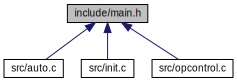
\includegraphics[width=309pt]{main_8h__dep__incl}
\end{center}
\end{figure}
\subsubsection*{Functions}
\begin{DoxyCompactItemize}
\item 
void \textbf{ autonomous} ()
\item 
void \textbf{ initialize} ()
\item 
void \textbf{ initialize\+IO} ()
\item 
void \textbf{ operator\+Control} ()
\end{DoxyCompactItemize}


\subsubsection{Detailed Description}
Header file for global functions. 

Any experienced C or C++ programmer knows the importance of header files. For those who do not, a header file allows multiple files to reference functions in other files without necessarily having to see the code (and therefore causing a multiple definition). To make a function in \char`\"{}opcontrol.\+c\char`\"{}, \char`\"{}auto.\+c\char`\"{}, \char`\"{}main.\+c\char`\"{}, or any other C file visible to the core implementation files, prototype it here.

This file is included by default in the predefined stubs in each V\+EX Cortex P\+R\+OS Project.

Copyright (c) 2011-\/2014, Purdue University A\+CM S\+IG B\+O\+TS. All rights reserved.

Redistribution and use in source and binary forms, with or without modification, are permitted provided that the following conditions are met\+:
\begin{DoxyItemize}
\item Redistributions of source code must retain the above copyright notice, this list of conditions and the following disclaimer.
\item Redistributions in binary form must reproduce the above copyright notice, this list of conditions and the following disclaimer in the documentation and/or other materials provided with the distribution.
\item Neither the name of Purdue University A\+CM S\+IG B\+O\+TS nor the names of its contributors may be used to endorse or promote products derived from this software without specific prior written permission.
\end{DoxyItemize}

T\+H\+IS S\+O\+F\+T\+W\+A\+RE IS P\+R\+O\+V\+I\+D\+ED BY T\+HE C\+O\+P\+Y\+R\+I\+G\+HT H\+O\+L\+D\+E\+RS A\+ND C\+O\+N\+T\+R\+I\+B\+U\+T\+O\+RS \char`\"{}\+A\+S I\+S\char`\"{} A\+ND A\+NY E\+X\+P\+R\+E\+SS OR I\+M\+P\+L\+I\+ED W\+A\+R\+R\+A\+N\+T\+I\+ES, I\+N\+C\+L\+U\+D\+I\+NG, B\+UT N\+OT L\+I\+M\+I\+T\+ED TO, T\+HE I\+M\+P\+L\+I\+ED W\+A\+R\+R\+A\+N\+T\+I\+ES OF M\+E\+R\+C\+H\+A\+N\+T\+A\+B\+I\+L\+I\+TY A\+ND F\+I\+T\+N\+E\+SS F\+OR A P\+A\+R\+T\+I\+C\+U\+L\+AR P\+U\+R\+P\+O\+SE A\+RE D\+I\+S\+C\+L\+A\+I\+M\+ED. IN NO E\+V\+E\+NT S\+H\+A\+LL P\+U\+R\+D\+UE U\+N\+I\+V\+E\+R\+S\+I\+TY A\+CM S\+IG B\+O\+TS BE L\+I\+A\+B\+LE F\+OR A\+NY D\+I\+R\+E\+CT, I\+N\+D\+I\+R\+E\+CT, I\+N\+C\+I\+D\+E\+N\+T\+AL, S\+P\+E\+C\+I\+AL, E\+X\+E\+M\+P\+L\+A\+RY, OR C\+O\+N\+S\+E\+Q\+U\+E\+N\+T\+I\+AL D\+A\+M\+A\+G\+ES (I\+N\+C\+L\+U\+D\+I\+NG, B\+UT N\+OT L\+I\+M\+I\+T\+ED TO, P\+R\+O\+C\+U\+R\+E\+M\+E\+NT OF S\+U\+B\+S\+T\+I\+T\+U\+TE G\+O\+O\+DS OR S\+E\+R\+V\+I\+C\+ES; L\+O\+SS OF U\+SE, D\+A\+TA, OR P\+R\+O\+F\+I\+TS; OR B\+U\+S\+I\+N\+E\+SS I\+N\+T\+E\+R\+R\+U\+P\+T\+I\+ON) H\+O\+W\+E\+V\+ER C\+A\+U\+S\+ED A\+ND ON A\+NY T\+H\+E\+O\+RY OF L\+I\+A\+B\+I\+L\+I\+TY, W\+H\+E\+T\+H\+ER IN C\+O\+N\+T\+R\+A\+CT, S\+T\+R\+I\+CT L\+I\+A\+B\+I\+L\+I\+TY, OR T\+O\+RT (I\+N\+C\+L\+U\+D\+I\+NG N\+E\+G\+L\+I\+G\+E\+N\+CE OR O\+T\+H\+E\+R\+W\+I\+SE) A\+R\+I\+S\+I\+NG IN A\+NY W\+AY O\+UT OF T\+HE U\+SE OF T\+H\+IS S\+O\+F\+T\+W\+A\+RE, E\+V\+EN IF A\+D\+V\+I\+S\+ED OF T\+HE P\+O\+S\+S\+I\+B\+I\+L\+I\+TY OF S\+U\+CH D\+A\+M\+A\+GE.

Purdue Robotics OS contains Free\+R\+T\+OS ({\tt http\+://www.\+freertos.\+org}) whose source code may be obtained from {\tt http\+://sourceforge.\+net/projects/freertos/files/} or on request. 

Definition in file \textbf{ main.\+h}.



\subsubsection{Function Documentation}
\mbox{\label{main_8h_a3c7ca506bbc071fa740de13805b7f376}} 
\index{main.\+h@{main.\+h}!autonomous@{autonomous}}
\index{autonomous@{autonomous}!main.\+h@{main.\+h}}
\paragraph{autonomous()}
{\footnotesize\ttfamily void autonomous (\begin{DoxyParamCaption}{ }\end{DoxyParamCaption})}

Runs the user autonomous code. This function will be started in its own task with the default priority and stack size whenever the robot is enabled via the Field Management System or the V\+EX Competition Switch in the autonomous mode. If the robot is disabled or communications is lost, the autonomous task will be stopped by the kernel. Re-\/enabling the robot will restart the task, not re-\/start it from where it left off.

Code running in the autonomous task cannot access information from the V\+EX Joystick. However, the autonomous function can be invoked from another task if a V\+EX Competition Switch is not available, and it can access joystick information if called in this way.

The autonomous task may exit, unlike \doxyref{operator\+Control()}{p.}{main_8h_ac71a94af413917f27d108e95c4d6f6a7} which should never exit. If it does so, the robot will await a switch to another mode or disable/enable cycle. 

Definition at line \textbf{ 30} of file \textbf{ auto.\+c}.



References \textbf{ analog\+Read()}, \textbf{ B\+O\+TH}, \textbf{ close\+\_\+claw()}, \textbf{ deinitslew()}, \textbf{ delay()}, \textbf{ G\+O\+A\+L\+\_\+\+H\+E\+I\+G\+HT}, \textbf{ ime\+Get()}, \textbf{ ime\+Reset()}, \textbf{ init\+\_\+slew()}, \textbf{ L\+I\+F\+T\+ER}, \textbf{ M\+I\+D\+\_\+\+L\+E\+F\+T\+\_\+\+D\+R\+I\+VE}, \textbf{ M\+I\+D\+\_\+\+R\+I\+G\+H\+T\+\_\+\+D\+R\+I\+VE}, \textbf{ open\+\_\+claw()}, \textbf{ printf()}, \textbf{ set\+\_\+lifter\+\_\+motors()}, and \textbf{ set\+\_\+side\+\_\+speed()}.


\begin{DoxyCode}
00030                   \{
00031   init_slew();
00032 
00033   delay(10);
00034   printf(\textcolor{stringliteral}{"auto\(\backslash\)n"});
00035   \textcolor{comment}{//How far the left wheels have gone}
00036   \textcolor{keywordtype}{int} counts\_drive\_left;
00037   \textcolor{comment}{//How far the right wheels have gone}
00038   \textcolor{keywordtype}{int} counts\_drive\_right;
00039   \textcolor{comment}{//The average distance traveled forward}
00040   \textcolor{keywordtype}{int} counts\_drive;
00041 
00042   \textcolor{comment}{//Reset the integrated motor controllers}
00043   imeReset(MID_LEFT_DRIVE);
00044   imeReset(MID_RIGHT_DRIVE);
00045   \textcolor{comment}{//Set initial values for how far the wheels have gone}
00046   imeGet(MID_LEFT_DRIVE, &counts\_drive\_left);
00047   imeGet(MID_RIGHT_DRIVE, &counts\_drive\_right);
00048   counts\_drive = counts\_drive\_left + counts\_drive\_right;
00049   counts\_drive /= 2;
00050 
00051   \textcolor{comment}{//Grab pre-load cone}
00052   close_claw();
00053   delay(300);
00054 
00055   \textcolor{comment}{//Raise the lifter}
00056   \textcolor{keywordflow}{while}(analogRead(LIFTER) < GOAL_HEIGHT)\{
00057     set_lifter_motors(-127);
00058   \}
00059   set_lifter_motors(0);
00060   \textcolor{comment}{//Drive towards the goal}
00061   \textcolor{keywordflow}{while}(counts\_drive < 530)\{
00062     set_side_speed(BOTH, 127);
00063     \textcolor{comment}{//Restablish the distance traveled}
00064     imeGet(MID_LEFT_DRIVE, &counts\_drive\_left);
00065     imeGet(MID_RIGHT_DRIVE, &counts\_drive\_right);
00066     counts\_drive = counts\_drive\_left + counts\_drive\_right;
00067     counts\_drive /= 2;
00068   \}
00069   \textcolor{comment}{//Stop moving}
00070   set_side_speed(BOTH, 0);
00071   delay(1000);
00072 
00073   \textcolor{comment}{//Drop the cone on the goal}
00074   open_claw();
00075   delay(1000);
00076   deinitslew();
00077 \}
\end{DoxyCode}
Here is the call graph for this function\+:\nopagebreak
\begin{figure}[H]
\begin{center}
\leavevmode
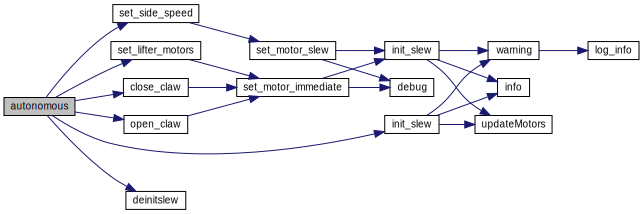
\includegraphics[width=350pt]{main_8h_a3c7ca506bbc071fa740de13805b7f376_cgraph}
\end{center}
\end{figure}
\mbox{\label{main_8h_a25a40b6614565f755233080a384c35f1}} 
\index{main.\+h@{main.\+h}!initialize@{initialize}}
\index{initialize@{initialize}!main.\+h@{main.\+h}}
\paragraph{initialize()}
{\footnotesize\ttfamily void initialize (\begin{DoxyParamCaption}{ }\end{DoxyParamCaption})}

Runs user initialization code. This function will be started in its own task with the default priority and stack size once when the robot is starting up. It is possible that the V\+E\+Xnet communication link may not be fully established at this time, so reading from the V\+EX Joystick may fail.

This function should initialize most sensors (gyro, encoders, ultrasonics), L\+C\+Ds, global variables, and I\+M\+Es.

This function must exit relatively promptly, or the \doxyref{operator\+Control()}{p.}{main_8h_ac71a94af413917f27d108e95c4d6f6a7} and \doxyref{autonomous()}{p.}{main_8h_a3c7ca506bbc071fa740de13805b7f376} tasks will not start. An autonomous mode selection menu like the pre\+\_\+auton() in other environments can be implemented in this task if desired. 

Definition at line \textbf{ 47} of file \textbf{ init.\+c}.



References \textbf{ ime\+Initialize\+All()}, \textbf{ printf()}, and \textbf{ set\+Team\+Name()}.


\begin{DoxyCode}
00047                   \{
00048   \textcolor{keywordtype}{int} c = imeInitializeAll();
00049   setTeamName(\textcolor{stringliteral}{"9228A"});
00050   printf(\textcolor{stringliteral}{"Counts : %d\(\backslash\)n"}, c);
00051 \}
\end{DoxyCode}
Here is the call graph for this function\+:\nopagebreak
\begin{figure}[H]
\begin{center}
\leavevmode
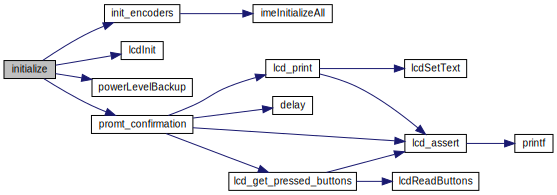
\includegraphics[width=248pt]{main_8h_a25a40b6614565f755233080a384c35f1_cgraph}
\end{center}
\end{figure}
\mbox{\label{main_8h_ad9cda921edb01125bb13c2f86bcf624b}} 
\index{main.\+h@{main.\+h}!initialize\+IO@{initialize\+IO}}
\index{initialize\+IO@{initialize\+IO}!main.\+h@{main.\+h}}
\paragraph{initialize\+I\+O()}
{\footnotesize\ttfamily void initialize\+IO (\begin{DoxyParamCaption}{ }\end{DoxyParamCaption})}

Runs pre-\/initialization code. This function will be started in kernel mode one time while the V\+EX Cortex is starting up. As the scheduler is still paused, most A\+PI functions will fail.

The purpose of this function is solely to set the default pin modes (\doxyref{pin\+Mode()}{p.}{_a_p_i_8h_a1875409d12eee562555bda94cad7f973}) and port states (\doxyref{digital\+Write()}{p.}{_a_p_i_8h_a23e767e5b47fa61d4e2cc02e6f15c7ab}) of limit switches, push buttons, and solenoids. It can also safely configure a U\+A\+RT port (usart\+Open()) but cannot set up an L\+CD (\doxyref{lcd\+Init()}{p.}{_a_p_i_8h_a43dc11a67b697c0d32315ea5a9af85f9}). 

Definition at line \textbf{ 30} of file \textbf{ init.\+c}.



References \textbf{ watchdog\+Init()}.


\begin{DoxyCode}
00030                     \{
00031     watchdogInit();
00032 \}
\end{DoxyCode}
Here is the call graph for this function\+:\nopagebreak
\begin{figure}[H]
\begin{center}
\leavevmode
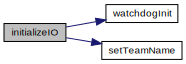
\includegraphics[width=250pt]{main_8h_ad9cda921edb01125bb13c2f86bcf624b_cgraph}
\end{center}
\end{figure}
\mbox{\label{main_8h_ac71a94af413917f27d108e95c4d6f6a7}} 
\index{main.\+h@{main.\+h}!operator\+Control@{operator\+Control}}
\index{operator\+Control@{operator\+Control}!main.\+h@{main.\+h}}
\paragraph{operator\+Control()}
{\footnotesize\ttfamily void operator\+Control (\begin{DoxyParamCaption}{ }\end{DoxyParamCaption})}

Runs the user operator control code. This function will be started in its own task with the default priority and stack size whenever the robot is enabled via the Field Management System or the V\+EX Competition Switch in the operator control mode. If the robot is disabled or communications is lost, the operator control task will be stopped by the kernel. Re-\/enabling the robot will restart the task, not resume it from where it left off.

If no V\+EX Competition Switch or Field Management system is plugged in, the V\+EX Cortex will run the operator control task. Be warned that this will also occur if the V\+EX Cortex is tethered directly to a computer via the U\+SB A to A cable without any V\+EX Joystick attached.

Code running in this task can take almost any action, as the V\+EX Joystick is available and the scheduler is operational. However, proper use of \doxyref{delay()}{p.}{_a_p_i_8h_a1c59207742a1acf45a8957d7f04f9dfe} or \doxyref{task\+Delay\+Until()}{p.}{_a_p_i_8h_ae93bc867b1aa4a12d6536a497f1b6869} is highly recommended to give other tasks (including system tasks such as updating L\+C\+Ds) time to run.

This task should never exit; it should end with some kind of infinite loop, even if empty. 

Definition at line \textbf{ 40} of file \textbf{ opcontrol.\+c}.



References \textbf{ delay()}, \textbf{ init\+\_\+slew()}, \textbf{ update\+\_\+claw()}, \textbf{ update\+\_\+control()}, \textbf{ update\+\_\+drive\+\_\+motors()}, \textbf{ update\+\_\+lifter()}, and \textbf{ update\+Intake()}.


\begin{DoxyCode}
00040                        \{
00041     init_slew();
00042     delay(10);
00043     \textcolor{keywordflow}{while} (1) \{
00044         update_drive_motors();
00045         update_lifter();
00046         update_claw();
00047         updateIntake();
00048         update_control();
00049         delay(25);
00050     \}
00051 \}
\end{DoxyCode}
Here is the call graph for this function\+:\nopagebreak
\begin{figure}[H]
\begin{center}
\leavevmode
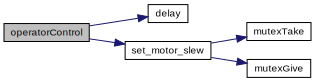
\includegraphics[width=350pt]{main_8h_ac71a94af413917f27d108e95c4d6f6a7_cgraph}
\end{center}
\end{figure}

\subsection{main.\+h}
\label{main_8h_source}\index{include/main.\+h@{include/main.\+h}}

\begin{DoxyCode}
00001 
00044 \textcolor{preprocessor}{#ifndef MAIN\_H\_}
00045 
00046 \textcolor{comment}{// This prevents multiple inclusion, which isn't bad for this file but is good}
00047 \textcolor{comment}{// practice}
00048 \textcolor{preprocessor}{#define MAIN\_H\_}
00049 
00050 \textcolor{preprocessor}{#include <API.h>}
00051 
00052 \textcolor{comment}{// Allow usage of this file in C++ programs}
00053 \textcolor{preprocessor}{#ifdef \_\_cplusplus}
00054 \textcolor{keyword}{extern} \textcolor{stringliteral}{"C"} \{
00055 \textcolor{preprocessor}{#endif}
00056 
00057 \textcolor{comment}{// Prototypes for initialization, operator control and autonomous}
00058 
00076 \textcolor{keywordtype}{void} autonomous();
00087 \textcolor{keywordtype}{void} initializeIO();
00101 \textcolor{keywordtype}{void} initialize();
00123 \textcolor{keywordtype}{void} operatorControl();
00124 
00125 \textcolor{comment}{// End C++ export structure}
00126 \textcolor{preprocessor}{#ifdef \_\_cplusplus}
00127 \}
00128 \textcolor{preprocessor}{#endif}
00129 
00130 \textcolor{preprocessor}{#endif}
\end{DoxyCode}

\section{include/matrix.h File Reference}
\label{matrix_8h}\index{include/matrix.\+h@{include/matrix.\+h}}


Various Matrix operations.

None of the matrix operations below change the input matrices if an input is required. They all return a new matrix with the new changes. Because memory issues are so prevelant, be sure to use the  function to reclaim some of that memory.  


This graph shows which files directly or indirectly include this file\+:\nopagebreak
\begin{figure}[H]
\begin{center}
\leavevmode
\includegraphics[width=315pt]{matrix_8h__dep__incl}
\end{center}
\end{figure}
\subsection*{Data Structures}
\begin{DoxyCompactItemize}
\item 
struct \textbf{ \+\_\+matrix}
\end{DoxyCompactItemize}
\subsection*{Typedefs}
\begin{DoxyCompactItemize}
\item 
typedef struct \textbf{ \+\_\+matrix} \textbf{ matrix}
\end{DoxyCompactItemize}
\subsection*{Functions}
\begin{DoxyCompactItemize}
\item 
void \textbf{ assert} (int assertion, const char $\ast$message)
\begin{DoxyCompactList}\small\item\em Asserts a condition is true. \end{DoxyCompactList}\item 
\textbf{ matrix} $\ast$ \textbf{ copy\+Matrix} (\textbf{ matrix} $\ast$m)
\begin{DoxyCompactList}\small\item\em Copies a matrix. This function uses scale\+Matrix, because scaling matrix by 1 is the same as a copy. \end{DoxyCompactList}\item 
\textbf{ matrix} $\ast$ \textbf{ covariance\+Matrix} (\textbf{ matrix} $\ast$m)
\begin{DoxyCompactList}\small\item\em returns the covariance of the matrix \end{DoxyCompactList}\item 
\textbf{ matrix} $\ast$ \textbf{ dot\+Diagonal\+Matrix} (\textbf{ matrix} $\ast$a, \textbf{ matrix} $\ast$b)
\begin{DoxyCompactList}\small\item\em performs a diagonial matrix dot product. Given a two matrices (or the same matrix twice) with identical widths and heights, this method returns a 1 by a-\/$>$height matrix of the cross product of each matrix along the diagonal. \end{DoxyCompactList}\item 
\textbf{ matrix} $\ast$ \textbf{ dot\+Product\+Matrix} (\textbf{ matrix} $\ast$a, \textbf{ matrix} $\ast$b)
\begin{DoxyCompactList}\small\item\em returns the matrix dot product. Given a two matrices (or the same matrix twice) with identical widths and different heights, this method returns a a-\/$>$height by b-\/$>$height matrix of the cross product of each matrix. \end{DoxyCompactList}\item 
void \textbf{ free\+Matrix} (\textbf{ matrix} $\ast$m)
\begin{DoxyCompactList}\small\item\em Frees the resources of a matrix. \end{DoxyCompactList}\item 
\textbf{ matrix} $\ast$ \textbf{ identity\+Matrix} (int n)
\begin{DoxyCompactList}\small\item\em Returns an identity matrix of size n by n. \end{DoxyCompactList}\item 
\textbf{ matrix} $\ast$ \textbf{ make\+Matrix} (int width, int height)
\begin{DoxyCompactList}\small\item\em Makes a matrix with a width and height parameters. \end{DoxyCompactList}\item 
\textbf{ matrix} $\ast$ \textbf{ mean\+Matrix} (\textbf{ matrix} $\ast$m)
\begin{DoxyCompactList}\small\item\em Given an \char`\"{}m rows by n columns\char`\"{} matrix, return a matrix where each element represents the mean of that full column.  the matrix. \end{DoxyCompactList}\item 
\textbf{ matrix} $\ast$ \textbf{ multiply\+Matrix} (\textbf{ matrix} $\ast$a, \textbf{ matrix} $\ast$b)
\begin{DoxyCompactList}\small\item\em Given a two matrices, returns the multiplication of the two. \end{DoxyCompactList}\item 
void \textbf{ print\+Matrix} (\textbf{ matrix} $\ast$m)
\begin{DoxyCompactList}\small\item\em Prints a matrix. \end{DoxyCompactList}\item 
void \textbf{ row\+Swap} (\textbf{ matrix} $\ast$a, int p, int q)
\begin{DoxyCompactList}\small\item\em swaps the rows of a matrix. This method changes the input matrix. Given a matrix, this algorithm will swap rows p and q, provided that p and q are less than or equal to the height of matrix A and p and q are different values. \end{DoxyCompactList}\item 
\textbf{ matrix} $\ast$ \textbf{ scale\+Matrix} (\textbf{ matrix} $\ast$m, double value)
\begin{DoxyCompactList}\small\item\em scales a matrix. \end{DoxyCompactList}\item 
double \textbf{ trace\+Matrix} (\textbf{ matrix} $\ast$m)
\begin{DoxyCompactList}\small\item\em Given an \char`\"{}m rows by n columns\char`\"{} matrix. \end{DoxyCompactList}\item 
\textbf{ matrix} $\ast$ \textbf{ transpose\+Matrix} (\textbf{ matrix} $\ast$m)
\begin{DoxyCompactList}\small\item\em returns the transpose matrix. \end{DoxyCompactList}\end{DoxyCompactItemize}


\subsection{Detailed Description}
Various Matrix operations.

None of the matrix operations below change the input matrices if an input is required. They all return a new matrix with the new changes. Because memory issues are so prevelant, be sure to use the  function to reclaim some of that memory. 



Definition in file \textbf{ matrix.\+h}.



\subsection{Typedef Documentation}
\mbox{\label{matrix_8h_abc75382643898dd572498a574bf891c7}} 
\index{matrix.\+h@{matrix.\+h}!matrix@{matrix}}
\index{matrix@{matrix}!matrix.\+h@{matrix.\+h}}
\subsubsection{matrix}
{\footnotesize\ttfamily typedef struct \textbf{ \+\_\+matrix}  \textbf{ matrix}}

A struct representing a matrix 

\subsection{Function Documentation}
\mbox{\label{matrix_8h_a8e41e30382335ea89f90b72db0b44d6f}} 
\index{matrix.\+h@{matrix.\+h}!assert@{assert}}
\index{assert@{assert}!matrix.\+h@{matrix.\+h}}
\subsubsection{assert()}
{\footnotesize\ttfamily void assert (\begin{DoxyParamCaption}\item[{int}]{assertion,  }\item[{const char $\ast$}]{message }\end{DoxyParamCaption})}



Asserts a condition is true. 

If the assertion is non-\/zero (i.\+e. true), then it returns. If the assertion is zero (i.\+e. false), then it display the string and aborts the program. This is ment to act like Python\textquotesingle{}s assert keyword. 

Definition at line \textbf{ 14} of file \textbf{ matrix.\+c}.



Referenced by \textbf{ covariance\+Matrix()}, \textbf{ dot\+Diagonal\+Matrix()}, \textbf{ dot\+Product\+Matrix()}, \textbf{ identity\+Matrix()}, \textbf{ make\+Matrix()}, \textbf{ mean\+Matrix()}, \textbf{ multiply\+Matrix()}, and \textbf{ row\+Swap()}.


\begin{DoxyCode}
00014                                                 \{
00015     \textcolor{keywordflow}{if} (assertion == 0) \{
00016         fprintf(stderr, \textcolor{stringliteral}{"%s\(\backslash\)n"}, message);
00017         exit(1);
00018     \}
00019 \}
\end{DoxyCode}
\mbox{\label{matrix_8h_abbb8d2d20c2dd53a2269d017a336668f}} 
\index{matrix.\+h@{matrix.\+h}!copy\+Matrix@{copy\+Matrix}}
\index{copy\+Matrix@{copy\+Matrix}!matrix.\+h@{matrix.\+h}}
\subsubsection{copy\+Matrix()}
{\footnotesize\ttfamily \textbf{ matrix}$\ast$ copy\+Matrix (\begin{DoxyParamCaption}\item[{\textbf{ matrix} $\ast$}]{m }\end{DoxyParamCaption})}



Copies a matrix. This function uses scale\+Matrix, because scaling matrix by 1 is the same as a copy. 


\begin{DoxyParams}{Parameters}
{\em m} & a pointer to the matrix \\
\hline
\end{DoxyParams}
\begin{DoxyReturn}{Returns}
a copied matrix 
\end{DoxyReturn}


Definition at line \textbf{ 52} of file \textbf{ matrix.\+c}.



References \textbf{ scale\+Matrix()}.


\begin{DoxyCode}
00052                               \{
00053     \textcolor{keywordflow}{return} scaleMatrix(m, 1);
00054 \}
\end{DoxyCode}
\mbox{\label{matrix_8h_ae6dab569959c360cf165136a3b625edd}} 
\index{matrix.\+h@{matrix.\+h}!covariance\+Matrix@{covariance\+Matrix}}
\index{covariance\+Matrix@{covariance\+Matrix}!matrix.\+h@{matrix.\+h}}
\subsubsection{covariance\+Matrix()}
{\footnotesize\ttfamily \textbf{ matrix}$\ast$ covariance\+Matrix (\begin{DoxyParamCaption}\item[{\textbf{ matrix} $\ast$}]{m }\end{DoxyParamCaption})}



returns the covariance of the matrix 


\begin{DoxyParams}{Parameters}
{\em the} & matrix \\
\hline
\end{DoxyParams}
\begin{DoxyReturn}{Returns}
a matrix with n row and n columns, where each element represents covariance of 2 columns. 
\end{DoxyReturn}


Definition at line \textbf{ 168} of file \textbf{ matrix.\+c}.



References \textbf{ assert()}, \textbf{ \+\_\+matrix\+::data}, \textbf{ free\+Matrix()}, \textbf{ \+\_\+matrix\+::height}, \textbf{ make\+Matrix()}, \textbf{ mean\+Matrix()}, and \textbf{ \+\_\+matrix\+::width}.


\begin{DoxyCode}
00168                                     \{
00169     \textcolor{keywordtype}{int} i, j, k = 0;
00170     matrix* out;
00171     matrix* mean;
00172     \textcolor{keywordtype}{double}* ptrA;
00173     \textcolor{keywordtype}{double}* ptrB;
00174     \textcolor{keywordtype}{double}* ptrOut;
00175 
00176     assert(m->height > 1, \textcolor{stringliteral}{"Height of matrix cannot be zero or one."});
00177 
00178     mean = meanMatrix(m);
00179     out = makeMatrix(m->width, m->width);
00180     ptrOut = out->data;
00181 
00182     \textcolor{keywordflow}{for} (i = 0; i < m->width; i++) \{
00183         \textcolor{keywordflow}{for} (j = 0; j < m->width; j++) \{
00184              ptrA = &m->data[i];
00185              ptrB = &m->data[j];
00186              *ptrOut = 0.0;
00187              \textcolor{keywordflow}{for} (k = 0; k < m->height; k++) \{
00188                  *ptrOut += (*ptrA - mean->data[i]) * (*ptrB - mean->data[j]);
00189                  ptrA += m->width;
00190                  ptrB += m->width;
00191              \}
00192              *ptrOut /= m->height - 1;
00193              ptrOut++;
00194         \}
00195     \}
00196 
00197     freeMatrix(mean);
00198     \textcolor{keywordflow}{return} out;
00199 \}
\end{DoxyCode}
\mbox{\label{matrix_8h_af49b525d7476c365833db9acd975e3a5}} 
\index{matrix.\+h@{matrix.\+h}!dot\+Diagonal\+Matrix@{dot\+Diagonal\+Matrix}}
\index{dot\+Diagonal\+Matrix@{dot\+Diagonal\+Matrix}!matrix.\+h@{matrix.\+h}}
\subsubsection{dot\+Diagonal\+Matrix()}
{\footnotesize\ttfamily \textbf{ matrix}$\ast$ dot\+Diagonal\+Matrix (\begin{DoxyParamCaption}\item[{\textbf{ matrix} $\ast$}]{a,  }\item[{\textbf{ matrix} $\ast$}]{b }\end{DoxyParamCaption})}



performs a diagonial matrix dot product. Given a two matrices (or the same matrix twice) with identical widths and heights, this method returns a 1 by a-\/$>$height matrix of the cross product of each matrix along the diagonal. 

Dot product is essentially the sum-\/of-\/squares of two vectors.

If the second paramter is N\+U\+LL, it is assumed that we are performing a cross product with itself. 
\begin{DoxyParams}{Parameters}
{\em a} & the first matrix \\
\hline
{\em b} & the second matrix \\
\hline
\end{DoxyParams}
\begin{DoxyReturn}{Returns}
the matrix result 
\end{DoxyReturn}


Definition at line \textbf{ 385} of file \textbf{ matrix.\+c}.



References \textbf{ assert()}, \textbf{ \+\_\+matrix\+::data}, \textbf{ \+\_\+matrix\+::height}, \textbf{ make\+Matrix()}, and \textbf{ \+\_\+matrix\+::width}.


\begin{DoxyCode}
00385                                                 \{
00386     matrix* out;
00387     \textcolor{keywordtype}{double}* ptrOut;
00388     \textcolor{keywordtype}{double}* ptrA;
00389     \textcolor{keywordtype}{double}* ptrB;
00390     \textcolor{keywordtype}{int} i, j;
00391 
00392     \textcolor{keywordflow}{if} (b != NULL) \{
00393         assert(a->width == b->width && a->height == b->height, \textcolor{stringliteral}{"Matrices must be of the same
       dimensionality."});
00394     \}
00395 
00396     \textcolor{comment}{// Are we computing the sum of squares of the same matrix?}
00397     \textcolor{keywordflow}{if} (a == b || b == NULL) \{
00398         b = a; \textcolor{comment}{// May not appear safe, but we can do this without risk of losing b.}
00399     \}
00400 
00401     out = makeMatrix(1, a->height);
00402     ptrOut = out->data;
00403     ptrA = a->data;
00404     ptrB = b->data;
00405 
00406     \textcolor{keywordflow}{for} (i = 0; i < a->height; i++) \{
00407         *ptrOut = 0;
00408         \textcolor{keywordflow}{for} (j = 0; j < a->width; j++) \{
00409             *ptrOut += *ptrA * *ptrB;
00410             ptrA++;
00411             ptrB++;
00412         \}
00413         ptrOut++;
00414     \}
00415 
00416     \textcolor{keywordflow}{return} out;
00417 \}
\end{DoxyCode}
\mbox{\label{matrix_8h_a0b568a64e81a56779c2141b424475976}} 
\index{matrix.\+h@{matrix.\+h}!dot\+Product\+Matrix@{dot\+Product\+Matrix}}
\index{dot\+Product\+Matrix@{dot\+Product\+Matrix}!matrix.\+h@{matrix.\+h}}
\subsubsection{dot\+Product\+Matrix()}
{\footnotesize\ttfamily \textbf{ matrix}$\ast$ dot\+Product\+Matrix (\begin{DoxyParamCaption}\item[{\textbf{ matrix} $\ast$}]{a,  }\item[{\textbf{ matrix} $\ast$}]{b }\end{DoxyParamCaption})}



returns the matrix dot product. Given a two matrices (or the same matrix twice) with identical widths and different heights, this method returns a a-\/$>$height by b-\/$>$height matrix of the cross product of each matrix. 

Dot product is essentially the sum-\/of-\/squares of two vectors.

Also, if the second paramter is N\+U\+LL, it is assumed that we are performing a cross product with itself. 
\begin{DoxyParams}{Parameters}
{\em a} & the first matrix \\
\hline
{\em the} & second matrix \\
\hline
\end{DoxyParams}
\begin{DoxyReturn}{Returns}
the result of the dot product 
\end{DoxyReturn}


Definition at line \textbf{ 333} of file \textbf{ matrix.\+c}.



References \textbf{ assert()}, \textbf{ \+\_\+matrix\+::data}, \textbf{ \+\_\+matrix\+::height}, \textbf{ make\+Matrix()}, and \textbf{ \+\_\+matrix\+::width}.


\begin{DoxyCode}
00333                                                \{
00334     matrix* out;
00335     \textcolor{keywordtype}{double}* ptrOut;
00336     \textcolor{keywordtype}{double}* ptrA;
00337     \textcolor{keywordtype}{double}* ptrB;
00338     \textcolor{keywordtype}{int} i, j, k;
00339 
00340     \textcolor{keywordflow}{if} (b != NULL) \{
00341         assert(a->width == b->width, \textcolor{stringliteral}{"Matrices must be of the same dimensionality."});
00342     \}
00343 
00344     \textcolor{comment}{// Are we computing the sum of squares of the same matrix?}
00345     \textcolor{keywordflow}{if} (a == b || b == NULL) \{
00346         b = a; \textcolor{comment}{// May not appear safe, but we can do this without risk of losing b.}
00347     \}
00348 
00349     out = makeMatrix(b->height, a->height);
00350     ptrOut = out->data;
00351 
00352     \textcolor{keywordflow}{for} (i = 0; i < a->height; i++) \{
00353         ptrB = b->data;
00354 
00355         \textcolor{keywordflow}{for} (j = 0; j < b->height; j++) \{
00356             ptrA = &a->data[ i * a->width ];
00357 
00358             *ptrOut = 0;
00359             \textcolor{keywordflow}{for} (k = 0; k < a->width; k++) \{
00360                 *ptrOut += *ptrA * *ptrB;
00361                 ptrA++;
00362                 ptrB++;
00363             \}
00364             ptrOut++;
00365         \}
00366     \}
00367 
00368     \textcolor{keywordflow}{return} out;
00369 \}
\end{DoxyCode}
\mbox{\label{matrix_8h_ae98365c910e9d688d2bdedec50d89a6b}} 
\index{matrix.\+h@{matrix.\+h}!free\+Matrix@{free\+Matrix}}
\index{free\+Matrix@{free\+Matrix}!matrix.\+h@{matrix.\+h}}
\subsubsection{free\+Matrix()}
{\footnotesize\ttfamily void free\+Matrix (\begin{DoxyParamCaption}\item[{\textbf{ matrix} $\ast$}]{m }\end{DoxyParamCaption})}



Frees the resources of a matrix. 


\begin{DoxyParams}{Parameters}
{\em the} & matrix to free \\
\hline
\end{DoxyParams}


Definition at line \textbf{ 60} of file \textbf{ matrix.\+c}.



References \textbf{ \+\_\+matrix\+::data}.



Referenced by \textbf{ covariance\+Matrix()}.


\begin{DoxyCode}
00060                            \{
00061     \textcolor{keywordflow}{if} (m != NULL) \{
00062         \textcolor{keywordflow}{if} (m->data != NULL) \{
00063             free(m->data);
00064             m->data = NULL;
00065         \}
00066         free(m);
00067     \}
00068     \textcolor{keywordflow}{return};
00069 \}
\end{DoxyCode}
\mbox{\label{matrix_8h_aa3f5e409b1641373be7cf7284e216d1a}} 
\index{matrix.\+h@{matrix.\+h}!identity\+Matrix@{identity\+Matrix}}
\index{identity\+Matrix@{identity\+Matrix}!matrix.\+h@{matrix.\+h}}
\subsubsection{identity\+Matrix()}
{\footnotesize\ttfamily \textbf{ matrix}$\ast$ identity\+Matrix (\begin{DoxyParamCaption}\item[{int}]{n }\end{DoxyParamCaption})}



Returns an identity matrix of size n by n. 


\begin{DoxyParams}{Parameters}
{\em n} & the input matrix. parameter.\\
\hline
{\em n} & the input matrix. \\
\hline
\end{DoxyParams}
\begin{DoxyReturn}{Returns}
the identity matrix parameter. 
\end{DoxyReturn}


Definition at line \textbf{ 94} of file \textbf{ matrix.\+c}.



References \textbf{ assert()}, \textbf{ \+\_\+matrix\+::data}, and \textbf{ make\+Matrix()}.


\begin{DoxyCode}
00094                               \{
00095     \textcolor{keywordtype}{int} i;
00096     matrix *out;
00097     \textcolor{keywordtype}{double}* ptr;
00098 
00099     assert(n > 0, \textcolor{stringliteral}{"Identity matrix must have value greater than zero."});
00100 
00101     out = makeMatrix(n, n);
00102     ptr = out->data;
00103     \textcolor{keywordflow}{for} (i = 0; i < n; i++) \{
00104         *ptr = 1.0;
00105         ptr += n + 1;
00106     \}
00107 
00108     \textcolor{keywordflow}{return} out;
00109 \}
\end{DoxyCode}
\mbox{\label{matrix_8h_aae8b56c6fb44d9147b835f4006ca872c}} 
\index{matrix.\+h@{matrix.\+h}!make\+Matrix@{make\+Matrix}}
\index{make\+Matrix@{make\+Matrix}!matrix.\+h@{matrix.\+h}}
\subsubsection{make\+Matrix()}
{\footnotesize\ttfamily \textbf{ matrix}$\ast$ make\+Matrix (\begin{DoxyParamCaption}\item[{int}]{width,  }\item[{int}]{height }\end{DoxyParamCaption})}



Makes a matrix with a width and height parameters. 


\begin{DoxyParams}{Parameters}
{\em width} & The width of the matrix \\
\hline
{\em height} & the height of the matrix \\
\hline
\end{DoxyParams}
\begin{DoxyReturn}{Returns}
the new matrix 
\end{DoxyReturn}


Definition at line \textbf{ 27} of file \textbf{ matrix.\+c}.



References \textbf{ assert()}, \textbf{ \+\_\+matrix\+::data}, \textbf{ \+\_\+matrix\+::height}, and \textbf{ \+\_\+matrix\+::width}.



Referenced by \textbf{ covariance\+Matrix()}, \textbf{ dot\+Diagonal\+Matrix()}, \textbf{ dot\+Product\+Matrix()}, \textbf{ identity\+Matrix()}, \textbf{ init\+\_\+localization()}, \textbf{ mean\+Matrix()}, \textbf{ multiply\+Matrix()}, \textbf{ scale\+Matrix()}, and \textbf{ transpose\+Matrix()}.


\begin{DoxyCode}
00027                                           \{
00028     matrix* out;
00029     assert(width > 0 && height > 0, \textcolor{stringliteral}{"New matrix must be at least a 1 by 1"});
00030     out = (matrix*) malloc(\textcolor{keyword}{sizeof}(matrix));
00031 
00032     assert(out != NULL, \textcolor{stringliteral}{"Out of memory."});
00033 
00034     out->width = width;
00035     out->height = height;
00036     out->data = (\textcolor{keywordtype}{double}*) malloc(\textcolor{keyword}{sizeof}(\textcolor{keywordtype}{double}) * width * height);
00037 
00038     assert(out->data != NULL, \textcolor{stringliteral}{"Out of memory."});
00039 
00040     memset(out->data, 0.0, width * height * \textcolor{keyword}{sizeof}(\textcolor{keywordtype}{double}));
00041 
00042     \textcolor{keywordflow}{return} out;
00043 \}
\end{DoxyCode}
\mbox{\label{matrix_8h_ae4babf9b518a2d5d6b12776191e3b7de}} 
\index{matrix.\+h@{matrix.\+h}!mean\+Matrix@{mean\+Matrix}}
\index{mean\+Matrix@{mean\+Matrix}!matrix.\+h@{matrix.\+h}}
\subsubsection{mean\+Matrix()}
{\footnotesize\ttfamily \textbf{ matrix}$\ast$ mean\+Matrix (\begin{DoxyParamCaption}\item[{\textbf{ matrix} $\ast$}]{m }\end{DoxyParamCaption})}



Given an \char`\"{}m rows by n columns\char`\"{} matrix, return a matrix where each element represents the mean of that full column.  the matrix. 

\begin{DoxyReturn}{Returns}
matrix with 1 row and n columns each element represents the mean of that full column. 
\end{DoxyReturn}


Definition at line \textbf{ 142} of file \textbf{ matrix.\+c}.



References \textbf{ assert()}, \textbf{ \+\_\+matrix\+::data}, \textbf{ \+\_\+matrix\+::height}, \textbf{ make\+Matrix()}, and \textbf{ \+\_\+matrix\+::width}.



Referenced by \textbf{ covariance\+Matrix()}.


\begin{DoxyCode}
00142                               \{
00143     \textcolor{keywordtype}{int} i, j;
00144     matrix* out;
00145 
00146     assert(m->height > 0, \textcolor{stringliteral}{"Height of matrix cannot be zero."});
00147 
00148     out = makeMatrix(m->width, 1);
00149 
00150     \textcolor{keywordflow}{for} (i = 0; i < m->width; i++) \{
00151         \textcolor{keywordtype}{double}* ptr;
00152         out->data[i] = 0.0;
00153         ptr = &m->data[i];
00154         \textcolor{keywordflow}{for} (j = 0; j < m->height; j++) \{
00155             out->data[i] += *ptr;
00156             ptr += out->width;
00157         \}
00158         out->data[i] /= (double) m->height;
00159     \}
00160     \textcolor{keywordflow}{return} out;
00161 \}
\end{DoxyCode}
\mbox{\label{matrix_8h_a63ed5c518b34768e9ef8e9d5f7d0b534}} 
\index{matrix.\+h@{matrix.\+h}!multiply\+Matrix@{multiply\+Matrix}}
\index{multiply\+Matrix@{multiply\+Matrix}!matrix.\+h@{matrix.\+h}}
\subsubsection{multiply\+Matrix()}
{\footnotesize\ttfamily \textbf{ matrix}$\ast$ multiply\+Matrix (\begin{DoxyParamCaption}\item[{\textbf{ matrix} $\ast$}]{a,  }\item[{\textbf{ matrix} $\ast$}]{b }\end{DoxyParamCaption})}



Given a two matrices, returns the multiplication of the two. 


\begin{DoxyParams}{Parameters}
{\em a} & the first matrix \\
\hline
{\em b} & the seconf matrix return the result of the multiplication \\
\hline
\end{DoxyParams}


Definition at line \textbf{ 230} of file \textbf{ matrix.\+c}.



References \textbf{ assert()}, \textbf{ \+\_\+matrix\+::data}, \textbf{ \+\_\+matrix\+::height}, \textbf{ make\+Matrix()}, and \textbf{ \+\_\+matrix\+::width}.


\begin{DoxyCode}
00230                                              \{
00231     \textcolor{keywordtype}{int} i, j, k;
00232     matrix* out;
00233     \textcolor{keywordtype}{double}* ptrOut;
00234     \textcolor{keywordtype}{double}* ptrA;
00235     \textcolor{keywordtype}{double}* ptrB;
00236 
00237     assert(a->width == b->height, \textcolor{stringliteral}{"Matrices have incorrect dimensions. a->width != b->height"});
00238 
00239     out = makeMatrix(b->width, a->height);
00240     ptrOut = out->data;
00241 
00242     \textcolor{keywordflow}{for} (i = 0; i < a->height; i++) \{
00243 
00244         \textcolor{keywordflow}{for} (j = 0; j < b->width; j++) \{
00245             ptrA = &a->data[ i * a->width ];
00246             ptrB = &b->data[ j ];
00247 
00248             *ptrOut = 0;
00249             \textcolor{keywordflow}{for} (k = 0; k < a->width; k++) \{
00250                 *ptrOut += *ptrA * *ptrB;
00251                 ptrA++;
00252                 ptrB += b->width;
00253             \}
00254             ptrOut++;
00255         \}
00256     \}
00257 
00258     \textcolor{keywordflow}{return} out;
00259 \}
\end{DoxyCode}
\mbox{\label{matrix_8h_a50ab2b1ac33d6993d93522fc4f30a051}} 
\index{matrix.\+h@{matrix.\+h}!print\+Matrix@{print\+Matrix}}
\index{print\+Matrix@{print\+Matrix}!matrix.\+h@{matrix.\+h}}
\subsubsection{print\+Matrix()}
{\footnotesize\ttfamily void print\+Matrix (\begin{DoxyParamCaption}\item[{\textbf{ matrix} $\ast$}]{m }\end{DoxyParamCaption})}



Prints a matrix. 


\begin{DoxyParams}{Parameters}
{\em the} & matrix \\
\hline
\end{DoxyParams}


Definition at line \textbf{ 75} of file \textbf{ matrix.\+c}.



References \textbf{ \+\_\+matrix\+::data}, \textbf{ \+\_\+matrix\+::height}, and \textbf{ \+\_\+matrix\+::width}.


\begin{DoxyCode}
00075                             \{
00076     \textcolor{keywordtype}{int} i, j;
00077     \textcolor{keywordtype}{double}* ptr = m->data;
00078     printf(\textcolor{stringliteral}{"%d %d\(\backslash\)n"}, m->width, m->height);
00079     \textcolor{keywordflow}{for} (i = 0; i < m->height; i++) \{
00080         \textcolor{keywordflow}{for} (j = 0; j < m->width; j++) \{
00081             printf(\textcolor{stringliteral}{" %9.6f"}, *(ptr++));
00082         \}
00083         printf(\textcolor{stringliteral}{"\(\backslash\)n"});
00084     \}
00085     \textcolor{keywordflow}{return};
00086 \}
\end{DoxyCode}
\mbox{\label{matrix_8h_acdd57777a972ce339153878fa917db14}} 
\index{matrix.\+h@{matrix.\+h}!row\+Swap@{row\+Swap}}
\index{row\+Swap@{row\+Swap}!matrix.\+h@{matrix.\+h}}
\subsubsection{row\+Swap()}
{\footnotesize\ttfamily void row\+Swap (\begin{DoxyParamCaption}\item[{\textbf{ matrix} $\ast$}]{a,  }\item[{int}]{p,  }\item[{int}]{q }\end{DoxyParamCaption})}



swaps the rows of a matrix. This method changes the input matrix. Given a matrix, this algorithm will swap rows p and q, provided that p and q are less than or equal to the height of matrix A and p and q are different values. 


\begin{DoxyParams}{Parameters}
{\em the} & matrix to swap. This method changes the input matrix. \\
\hline
{\em the} & first row \\
\hline
{\em the} & second row \\
\hline
\end{DoxyParams}


Definition at line \textbf{ 290} of file \textbf{ matrix.\+c}.



References \textbf{ assert()}, \textbf{ \+\_\+matrix\+::data}, \textbf{ \+\_\+matrix\+::height}, and \textbf{ \+\_\+matrix\+::width}.


\begin{DoxyCode}
00290                                       \{
00291     \textcolor{keywordtype}{int} i;
00292     \textcolor{keywordtype}{double} temp;
00293     \textcolor{keywordtype}{double}* pRow;
00294     \textcolor{keywordtype}{double}* qRow;
00295 
00296     assert(a->height > 2, \textcolor{stringliteral}{"Matrix must have at least two rows to swap."});
00297     assert(p < a->height && q < a->height, \textcolor{stringliteral}{"Values p and q must be less than the height of the matrix."});
00298 
00299     \textcolor{comment}{// If p and q are equal, do nothing.}
00300     \textcolor{keywordflow}{if} (p == q) \{
00301         \textcolor{keywordflow}{return};
00302     \}
00303 
00304     pRow = a->data + (p * a->width);
00305     qRow = a->data + (q * a->width);
00306 
00307     \textcolor{comment}{// Swap!}
00308     \textcolor{keywordflow}{for} (i = 0; i < a->width; i++) \{
00309         temp = *pRow;
00310         *pRow = *qRow;
00311         *qRow = temp;
00312         pRow++;
00313         qRow++;
00314     \}
00315 
00316     \textcolor{keywordflow}{return};
00317 \}
\end{DoxyCode}
\mbox{\label{matrix_8h_a6b7faa6ba9ee987d0777d9d0bd0e7b32}} 
\index{matrix.\+h@{matrix.\+h}!scale\+Matrix@{scale\+Matrix}}
\index{scale\+Matrix@{scale\+Matrix}!matrix.\+h@{matrix.\+h}}
\subsubsection{scale\+Matrix()}
{\footnotesize\ttfamily \textbf{ matrix}$\ast$ scale\+Matrix (\begin{DoxyParamCaption}\item[{\textbf{ matrix} $\ast$}]{m,  }\item[{double}]{value }\end{DoxyParamCaption})}



scales a matrix. 


\begin{DoxyParams}{Parameters}
{\em m} & the matrix to scale \\
\hline
{\em the} & value to scale by \\
\hline
\end{DoxyParams}
\begin{DoxyReturn}{Returns}
a new matrix where each element in the input matrix is multiplied by the scalar value 
\end{DoxyReturn}


Definition at line \textbf{ 268} of file \textbf{ matrix.\+c}.



References \textbf{ \+\_\+matrix\+::data}, \textbf{ \+\_\+matrix\+::height}, \textbf{ make\+Matrix()}, and \textbf{ \+\_\+matrix\+::width}.



Referenced by \textbf{ copy\+Matrix()}.


\begin{DoxyCode}
00268                                              \{
00269     \textcolor{keywordtype}{int} i, elements = m->width * m->height;
00270     matrix* out = makeMatrix(m->width, m->height);
00271     \textcolor{keywordtype}{double}* ptrM = m->data;
00272     \textcolor{keywordtype}{double}* ptrOut = out->data;
00273 
00274     \textcolor{keywordflow}{for} (i = 0; i < elements; i++) \{
00275         *(ptrOut++) = *(ptrM++) * value;
00276     \}
00277 
00278     \textcolor{keywordflow}{return} out;
00279 \}
\end{DoxyCode}
\mbox{\label{matrix_8h_a4794df8b2032f961dd8b2d90276bc417}} 
\index{matrix.\+h@{matrix.\+h}!trace\+Matrix@{trace\+Matrix}}
\index{trace\+Matrix@{trace\+Matrix}!matrix.\+h@{matrix.\+h}}
\subsubsection{trace\+Matrix()}
{\footnotesize\ttfamily double trace\+Matrix (\begin{DoxyParamCaption}\item[{\textbf{ matrix} $\ast$}]{m }\end{DoxyParamCaption})}



Given an \char`\"{}m rows by n columns\char`\"{} matrix. 

\begin{DoxyReturn}{Returns}
the sum of the elements along the diagonal.
\end{DoxyReturn}
Given an \char`\"{}m rows by n columns\char`\"{} matrix.

\begin{DoxyReturn}{Returns}
the sum of the elements along the diagonal. 
\end{DoxyReturn}


Definition at line \textbf{ 116} of file \textbf{ matrix.\+c}.



References \textbf{ \+\_\+matrix\+::data}, \textbf{ \+\_\+matrix\+::height}, and \textbf{ \+\_\+matrix\+::width}.


\begin{DoxyCode}
00116                               \{
00117     \textcolor{keywordtype}{int} i;
00118     \textcolor{keywordtype}{int} size;
00119     \textcolor{keywordtype}{double}* ptr = m->data;
00120     \textcolor{keywordtype}{double} sum = 0.0;
00121 
00122     \textcolor{keywordflow}{if} (m->height < m->width) \{
00123         size = m->height;
00124     \}
00125     \textcolor{keywordflow}{else} \{
00126         size = m->width;
00127     \}
00128 
00129     \textcolor{keywordflow}{for} (i = 0; i < size; i++) \{
00130         sum += *ptr;
00131         ptr += m->width + 1;
00132     \}
00133 
00134     \textcolor{keywordflow}{return} sum;
00135 \}
\end{DoxyCode}
\mbox{\label{matrix_8h_a2936260302742748b0639e8ec71d4d9f}} 
\index{matrix.\+h@{matrix.\+h}!transpose\+Matrix@{transpose\+Matrix}}
\index{transpose\+Matrix@{transpose\+Matrix}!matrix.\+h@{matrix.\+h}}
\subsubsection{transpose\+Matrix()}
{\footnotesize\ttfamily \textbf{ matrix}$\ast$ transpose\+Matrix (\begin{DoxyParamCaption}\item[{\textbf{ matrix} $\ast$}]{m }\end{DoxyParamCaption})}



returns the transpose matrix. 


\begin{DoxyParams}{Parameters}
{\em the} & matrix to transpose. \\
\hline
\end{DoxyParams}
\begin{DoxyReturn}{Returns}
the transposed matrix. 
\end{DoxyReturn}


Definition at line \textbf{ 206} of file \textbf{ matrix.\+c}.



References \textbf{ \+\_\+matrix\+::data}, \textbf{ \+\_\+matrix\+::height}, \textbf{ make\+Matrix()}, and \textbf{ \+\_\+matrix\+::width}.


\begin{DoxyCode}
00206                                    \{
00207     matrix* out = makeMatrix(m->height, m->width);
00208     \textcolor{keywordtype}{double}* ptrM = m->data;
00209     \textcolor{keywordtype}{int} i, j;
00210 
00211     \textcolor{keywordflow}{for} (i = 0; i < m->height; i++) \{
00212         \textcolor{keywordtype}{double}* ptrOut;
00213         ptrOut = &out->data[i];
00214         \textcolor{keywordflow}{for} (j = 0; j < m->width; j++) \{
00215             *ptrOut = *ptrM;
00216             ptrM++;
00217             ptrOut += out->width;
00218         \}
00219     \}
00220 
00221     \textcolor{keywordflow}{return} out;
00222 \}
\end{DoxyCode}

\subsection{matrix.\+h}
\label{matrix_8h_source}\index{include/matrix.\+h@{include/matrix.\+h}}

\begin{DoxyCode}
00001 
00010 \textcolor{preprocessor}{#ifndef \_MATRIX\_H\_}
00011 \textcolor{preprocessor}{#define \_MATRIX\_H\_}
00012 
00016 \textcolor{keyword}{typedef} \textcolor{keyword}{struct }_matrix \{
00017   \textcolor{keywordtype}{int} height;
00018   \textcolor{keywordtype}{int} width;
00019   \textcolor{keywordtype}{double} *data;
00020 \} matrix;
00021 
00030 \textcolor{keywordtype}{void} assert(\textcolor{keywordtype}{int} assertion, \textcolor{keyword}{const} \textcolor{keywordtype}{char} *message);
00031 
00035 matrix *makeMatrix(\textcolor{keywordtype}{int} width, \textcolor{keywordtype}{int} height);
00036 
00044 matrix *copyMatrix(matrix *m);
00045 
00050 \textcolor{keywordtype}{void} freeMatrix(matrix *m);
00051 
00056 \textcolor{keywordtype}{void} printMatrix(matrix *m);
00057 
00063 matrix *identityMatrix(\textcolor{keywordtype}{int} n);
00064 
00070 \textcolor{keywordtype}{double} traceMatrix(matrix *m);
00071 
00077 matrix *transposeMatrix(matrix *m);
00078 
00086 matrix *meanMatrix(matrix *m);
00087 
00094 matrix *multiplyMatrix(matrix *a, matrix *b);
00095 
00103 matrix *scaleMatrix(matrix *m, \textcolor{keywordtype}{double} value);
00104 
00111 matrix *covarianceMatrix(matrix *m);
00112 
00122 \textcolor{keywordtype}{void} rowSwap(matrix *a, \textcolor{keywordtype}{int} p, \textcolor{keywordtype}{int} q);
00137 matrix *dotProductMatrix(matrix *a, matrix *b);
00138 
00153 matrix *dotDiagonalMatrix(matrix *a, matrix *b);
00154 
00155 \textcolor{preprocessor}{#endif}
\end{DoxyCode}

\hypertarget{menu_8h}{}\section{include/menu.h File Reference}
\label{menu_8h}\index{include/menu.\+h@{include/menu.\+h}}
{\ttfamily \#include \char`\"{}stdarg.\+h\char`\"{}}\newline
{\ttfamily \#include \char`\"{}stdlib.\+h\char`\"{}}\newline
{\ttfamily \#include $<$A\+P\+I.\+h$>$}\newline
{\ttfamily \#include \char`\"{}lcd.\+h\char`\"{}}\newline
Include dependency graph for menu.\+h\+:
% FIG 0
\subsection*{Data Structures}
\begin{DoxyCompactItemize}
\item 
struct \hyperlink{structmenu}{menu}
\item 
struct \hyperlink{structmenu__result}{menu\+\_\+result}
\end{DoxyCompactItemize}
\subsection*{Enumerations}
\begin{DoxyCompactItemize}
\item 
enum \hyperlink{menu_8h_a6bbf4baf5018b0d76aab6c2e6bf85e62}{menu\+\_\+type} \{ \hyperlink{menu_8h_a6bbf4baf5018b0d76aab6c2e6bf85e62a1762bddf438155a00ecf0318446e8a83}{int\+\_\+type}, 
\hyperlink{menu_8h_a6bbf4baf5018b0d76aab6c2e6bf85e62a67a95930928f80abf404f492d8ab0e22}{float\+\_\+type}, 
\hyperlink{menu_8h_a6bbf4baf5018b0d76aab6c2e6bf85e62afca80dc288f5f112ad3b5a8493758095}{string\+\_\+type}
 \}
\end{DoxyCompactItemize}
\subsection*{Functions}
\begin{DoxyCompactItemize}
\item 
struct \hyperlink{structmenu}{menu} $\ast$ \hyperlink{menu_8h_ad278f2d3a0219659e7cdfb3389dd7040}{init\+\_\+menu} (enum \hyperlink{menu_8h_a6bbf4baf5018b0d76aab6c2e6bf85e62}{menu\+\_\+type} type, unsigned int nums, char $\ast$options,...)
\item 
struct \hyperlink{structmenu}{menu} $\ast$ \hyperlink{menu_8h_a684f321ba7d9e2bab78f2025641faa79}{init\+\_\+menu} (enum \hyperlink{menu_8h_a6bbf4baf5018b0d76aab6c2e6bf85e62}{menu\+\_\+type} type, char $\ast$$\ast$options, unsigned int length)
\item 
struct \hyperlink{structmenu}{menu} $\ast$ \hyperlink{menu_8h_a0f38ebcd231151bda773bad9b08d17f2}{init\+\_\+menu} (enum \hyperlink{menu_8h_a6bbf4baf5018b0d76aab6c2e6bf85e62}{menu\+\_\+type} type, int min, int max, int step)
\item 
struct \hyperlink{structmenu}{menu} $\ast$ \hyperlink{menu_8h_ab0b05be4bdb1ef6554187247e50cc96f}{init\+\_\+menu} (enum \hyperlink{menu_8h_a6bbf4baf5018b0d76aab6c2e6bf85e62}{menu\+\_\+type} type, float min, float max, float step)
\item 
struct \hyperlink{structmenu__result}{menu\+\_\+result} \hyperlink{menu_8h_aee3e9f838cdbb1745c68974490aabb99}{display\+\_\+menu} (struct \hyperlink{structmenu}{menu} $\ast$\hyperlink{structmenu}{menu})
\item 
void \hyperlink{menu_8h_a84f7c6b4cde1e723a08937762cacc617}{denint\+\_\+menu} (struct \hyperlink{structmenu}{menu} $\ast$\hyperlink{structmenu}{menu})
\end{DoxyCompactItemize}


\subsection{Enumeration Type Documentation}
\mbox{\Hypertarget{menu_8h_a6bbf4baf5018b0d76aab6c2e6bf85e62}\label{menu_8h_a6bbf4baf5018b0d76aab6c2e6bf85e62}} 
\index{menu.\+h@{menu.\+h}!menu\+\_\+type@{menu\+\_\+type}}
\index{menu\+\_\+type@{menu\+\_\+type}!menu.\+h@{menu.\+h}}
\subsubsection{\texorpdfstring{menu\+\_\+type}{menu\_type}}
{\footnotesize\ttfamily enum \hyperlink{menu_8h_a6bbf4baf5018b0d76aab6c2e6bf85e62}{menu\+\_\+type}}

\begin{DoxyEnumFields}{Enumerator}
\raisebox{\heightof{T}}[0pt][0pt]{\index{int\+\_\+type@{int\+\_\+type}!menu.\+h@{menu.\+h}}\index{menu.\+h@{menu.\+h}!int\+\_\+type@{int\+\_\+type}}}\mbox{\Hypertarget{menu_8h_a6bbf4baf5018b0d76aab6c2e6bf85e62a1762bddf438155a00ecf0318446e8a83}\label{menu_8h_a6bbf4baf5018b0d76aab6c2e6bf85e62a1762bddf438155a00ecf0318446e8a83}} 
int\+\_\+type&\\
\hline

\raisebox{\heightof{T}}[0pt][0pt]{\index{float\+\_\+type@{float\+\_\+type}!menu.\+h@{menu.\+h}}\index{menu.\+h@{menu.\+h}!float\+\_\+type@{float\+\_\+type}}}\mbox{\Hypertarget{menu_8h_a6bbf4baf5018b0d76aab6c2e6bf85e62a67a95930928f80abf404f492d8ab0e22}\label{menu_8h_a6bbf4baf5018b0d76aab6c2e6bf85e62a67a95930928f80abf404f492d8ab0e22}} 
float\+\_\+type&\\
\hline

\raisebox{\heightof{T}}[0pt][0pt]{\index{string\+\_\+type@{string\+\_\+type}!menu.\+h@{menu.\+h}}\index{menu.\+h@{menu.\+h}!string\+\_\+type@{string\+\_\+type}}}\mbox{\Hypertarget{menu_8h_a6bbf4baf5018b0d76aab6c2e6bf85e62afca80dc288f5f112ad3b5a8493758095}\label{menu_8h_a6bbf4baf5018b0d76aab6c2e6bf85e62afca80dc288f5f112ad3b5a8493758095}} 
string\+\_\+type&\\
\hline

\end{DoxyEnumFields}


Definition at line 9 of file menu.\+h.



\subsection{Function Documentation}
\mbox{\Hypertarget{menu_8h_a84f7c6b4cde1e723a08937762cacc617}\label{menu_8h_a84f7c6b4cde1e723a08937762cacc617}} 
\index{menu.\+h@{menu.\+h}!denint\+\_\+menu@{denint\+\_\+menu}}
\index{denint\+\_\+menu@{denint\+\_\+menu}!menu.\+h@{menu.\+h}}
\subsubsection{\texorpdfstring{denint\+\_\+menu()}{denint\_menu()}}
{\footnotesize\ttfamily void denint\+\_\+menu (\begin{DoxyParamCaption}\item[{struct \hyperlink{structmenu}{menu} $\ast$}]{menu }\end{DoxyParamCaption})}



Definition at line 91 of file menu.\+h.

\mbox{\Hypertarget{menu_8h_aee3e9f838cdbb1745c68974490aabb99}\label{menu_8h_aee3e9f838cdbb1745c68974490aabb99}} 
\index{menu.\+h@{menu.\+h}!display\+\_\+menu@{display\+\_\+menu}}
\index{display\+\_\+menu@{display\+\_\+menu}!menu.\+h@{menu.\+h}}
\subsubsection{\texorpdfstring{display\+\_\+menu()}{display\_menu()}}
{\footnotesize\ttfamily struct \hyperlink{structmenu__result}{menu\+\_\+result} display\+\_\+menu (\begin{DoxyParamCaption}\item[{struct \hyperlink{structmenu}{menu} $\ast$}]{menu }\end{DoxyParamCaption})}



Definition at line 76 of file menu.\+h.

Here is the call graph for this function\+:
% FIG 1
\mbox{\Hypertarget{menu_8h_ad278f2d3a0219659e7cdfb3389dd7040}\label{menu_8h_ad278f2d3a0219659e7cdfb3389dd7040}} 
\index{menu.\+h@{menu.\+h}!init\+\_\+menu@{init\+\_\+menu}}
\index{init\+\_\+menu@{init\+\_\+menu}!menu.\+h@{menu.\+h}}
\subsubsection{\texorpdfstring{init\+\_\+menu()}{init\_menu()}\hspace{0.1cm}{\footnotesize\ttfamily [1/4]}}
{\footnotesize\ttfamily struct \hyperlink{structmenu}{menu}$\ast$ init\+\_\+menu (\begin{DoxyParamCaption}\item[{enum \hyperlink{menu_8h_a6bbf4baf5018b0d76aab6c2e6bf85e62}{menu\+\_\+type}}]{type,  }\item[{unsigned int}]{nums,  }\item[{char $\ast$}]{options,  }\item[{}]{... }\end{DoxyParamCaption})}



Definition at line 39 of file menu.\+h.

\mbox{\Hypertarget{menu_8h_a684f321ba7d9e2bab78f2025641faa79}\label{menu_8h_a684f321ba7d9e2bab78f2025641faa79}} 
\index{menu.\+h@{menu.\+h}!init\+\_\+menu@{init\+\_\+menu}}
\index{init\+\_\+menu@{init\+\_\+menu}!menu.\+h@{menu.\+h}}
\subsubsection{\texorpdfstring{init\+\_\+menu()}{init\_menu()}\hspace{0.1cm}{\footnotesize\ttfamily [2/4]}}
{\footnotesize\ttfamily struct \hyperlink{structmenu}{menu}$\ast$ init\+\_\+menu (\begin{DoxyParamCaption}\item[{enum \hyperlink{menu_8h_a6bbf4baf5018b0d76aab6c2e6bf85e62}{menu\+\_\+type}}]{type,  }\item[{char $\ast$$\ast$}]{options,  }\item[{unsigned int}]{length }\end{DoxyParamCaption})}



Definition at line 53 of file menu.\+h.

\mbox{\Hypertarget{menu_8h_a0f38ebcd231151bda773bad9b08d17f2}\label{menu_8h_a0f38ebcd231151bda773bad9b08d17f2}} 
\index{menu.\+h@{menu.\+h}!init\+\_\+menu@{init\+\_\+menu}}
\index{init\+\_\+menu@{init\+\_\+menu}!menu.\+h@{menu.\+h}}
\subsubsection{\texorpdfstring{init\+\_\+menu()}{init\_menu()}\hspace{0.1cm}{\footnotesize\ttfamily [3/4]}}
{\footnotesize\ttfamily struct \hyperlink{structmenu}{menu}$\ast$ init\+\_\+menu (\begin{DoxyParamCaption}\item[{enum \hyperlink{menu_8h_a6bbf4baf5018b0d76aab6c2e6bf85e62}{menu\+\_\+type}}]{type,  }\item[{int}]{min,  }\item[{int}]{max,  }\item[{int}]{step }\end{DoxyParamCaption})}



Definition at line 60 of file menu.\+h.

\mbox{\Hypertarget{menu_8h_ab0b05be4bdb1ef6554187247e50cc96f}\label{menu_8h_ab0b05be4bdb1ef6554187247e50cc96f}} 
\index{menu.\+h@{menu.\+h}!init\+\_\+menu@{init\+\_\+menu}}
\index{init\+\_\+menu@{init\+\_\+menu}!menu.\+h@{menu.\+h}}
\subsubsection{\texorpdfstring{init\+\_\+menu()}{init\_menu()}\hspace{0.1cm}{\footnotesize\ttfamily [4/4]}}
{\footnotesize\ttfamily struct \hyperlink{structmenu}{menu}$\ast$ init\+\_\+menu (\begin{DoxyParamCaption}\item[{enum \hyperlink{menu_8h_a6bbf4baf5018b0d76aab6c2e6bf85e62}{menu\+\_\+type}}]{type,  }\item[{float}]{min,  }\item[{float}]{max,  }\item[{float}]{step }\end{DoxyParamCaption})}



Definition at line 68 of file menu.\+h.


\subsection{menu.\+h}
\label{menu_8h_source}\index{include/menu.\+h@{include/menu.\+h}}

\begin{DoxyCode}
00001 
00008 \textcolor{preprocessor}{#ifndef \_MENU\_H\_}
00009 \textcolor{preprocessor}{#define \_MENU\_H\_}
00010 
00011 \textcolor{preprocessor}{#include "API.h"}
00012 \textcolor{preprocessor}{#include "lcd.h"}
00013 \textcolor{preprocessor}{#include <float.h>}
00014 \textcolor{preprocessor}{#include <limits.h>}
00015 \textcolor{preprocessor}{#include <string.h>}
00016 \textcolor{preprocessor}{#include <vlib.h>}
00017 \textcolor{preprocessor}{#include "log.h"}
00018 
00030 \textcolor{keyword}{enum} menu_type \{
00037   INT_TYPE,
00044   FLOAT_TYPE,
00050   STRING_TYPE
00051 \};
00052 
00066 \textcolor{keyword}{typedef} \textcolor{keyword}{struct }menu_t \{
00072   \textcolor{keyword}{enum} menu_type type;
00073 
00079   \textcolor{keywordtype}{char} **options;
00080 
00086   \textcolor{keywordtype}{unsigned} \textcolor{keywordtype}{int} length;
00087 
00094   \textcolor{keywordtype}{int} min;
00095 
00102   \textcolor{keywordtype}{int} max;
00103 
00111   \textcolor{keywordtype}{int} step;
00112 
00119   \textcolor{keywordtype}{float} min_f;
00120 
00127   \textcolor{keywordtype}{float} max_f;
00128 
00136   \textcolor{keywordtype}{float} step_f;
00142   \textcolor{keywordtype}{int} current;
00150   \textcolor{keywordtype}{char} *prompt;
00151 \} menu_t;
00152 
00165 menu_t *init_menu_var(\textcolor{keyword}{enum} menu_type type, \textcolor{keyword}{const} \textcolor{keywordtype}{char} *prompt, \textcolor{keywordtype}{int} nums, ...);
00166 
00180 menu_t *init_menu_int(\textcolor{keyword}{enum} menu_type type, \textcolor{keywordtype}{int} min, \textcolor{keywordtype}{int} max, \textcolor{keywordtype}{int} step,
00181                       \textcolor{keyword}{const} \textcolor{keywordtype}{char} *prompt);
00182 
00196 menu_t *init_menu_float(\textcolor{keyword}{enum} menu_type type, \textcolor{keywordtype}{float} min, \textcolor{keywordtype}{float} max, \textcolor{keywordtype}{float} step,
00197                         \textcolor{keyword}{const} \textcolor{keywordtype}{char} *prompt);
00198 
00209 \textcolor{keywordtype}{int} display_menu(menu_t *menu);
00210 
00220 \textcolor{keywordtype}{void} denint_menu(menu_t *menu);
00221 
00222 \textcolor{preprocessor}{#endif}
\end{DoxyCode}

\hypertarget{mobile__goal__intake_8h}{}\section{include/mobile\+\_\+goal\+\_\+intake.h File Reference}
\label{mobile__goal__intake_8h}\index{include/mobile\+\_\+goal\+\_\+intake.\+h@{include/mobile\+\_\+goal\+\_\+intake.\+h}}
{\ttfamily \#include \char`\"{}motor\+\_\+ports.\+h\char`\"{}}\newline
{\ttfamily \#include \char`\"{}controller.\+h\char`\"{}}\newline
{\ttfamily \#include \char`\"{}slew.\+h\char`\"{}}\newline
Include dependency graph for mobile\+\_\+goal\+\_\+intake.\+h\+:\nopagebreak
\begin{figure}[H]
\begin{center}
\leavevmode
\includegraphics[width=350pt]{mobile__goal__intake_8h__incl}
\end{center}
\end{figure}
This graph shows which files directly or indirectly include this file\+:\nopagebreak
\begin{figure}[H]
\begin{center}
\leavevmode
\includegraphics[width=306pt]{mobile__goal__intake_8h__dep__incl}
\end{center}
\end{figure}
\subsection*{Functions}
\begin{DoxyCompactItemize}
\item 
void \hyperlink{mobile__goal__intake_8h_ad0232c21c5c1ffda603d2b7d61034118}{update\+Intake} ()
\end{DoxyCompactItemize}


\subsection{Function Documentation}
\mbox{\Hypertarget{mobile__goal__intake_8h_ad0232c21c5c1ffda603d2b7d61034118}\label{mobile__goal__intake_8h_ad0232c21c5c1ffda603d2b7d61034118}} 
\index{mobile\+\_\+goal\+\_\+intake.\+h@{mobile\+\_\+goal\+\_\+intake.\+h}!update\+Intake@{update\+Intake}}
\index{update\+Intake@{update\+Intake}!mobile\+\_\+goal\+\_\+intake.\+h@{mobile\+\_\+goal\+\_\+intake.\+h}}
\subsubsection{\texorpdfstring{update\+Intake()}{updateIntake()}}
{\footnotesize\ttfamily void update\+Intake (\begin{DoxyParamCaption}{ }\end{DoxyParamCaption})}



Definition at line 16 of file mobile\+\_\+goal\+\_\+intake.\+c.



References get\+\_\+mode(), J\+O\+Y\+\_\+\+D\+O\+WN, J\+O\+Y\+\_\+\+UP, joystick\+Get\+Digital(), lower\+\_\+intake(), M\+A\+I\+N\+\_\+\+C\+O\+N\+T\+R\+O\+L\+L\+E\+R\+\_\+\+M\+O\+DE, M\+A\+S\+T\+ER, P\+A\+R\+T\+N\+ER, P\+A\+R\+T\+N\+E\+R\+\_\+\+C\+O\+N\+T\+R\+O\+L\+L\+E\+R\+\_\+\+M\+O\+DE, raise\+\_\+intake(), and set\+\_\+intake\+\_\+motor().



Referenced by operator\+Control().


\begin{DoxyCode}
16                     \{
17   \textcolor{keywordflow}{if}(\hyperlink{_a_p_i_8h_a792f1a80c62a63e764cf64aabf95db92}{joystickGetDigital}(\hyperlink{controller_8h_a3fa2d3bf1901157f734a584d47b25d8b}{MASTER}, 7, \hyperlink{_a_p_i_8h_a85e47af11e6a32e3a819f247d9f619d6}{JOY\_UP}) && (
      \hyperlink{partner_8h_aacc86d07e59d3b919f5c5eae2ce5d404}{get\_mode}() == \hyperlink{partner_8h_afb2b5bca5ceab5f6efd8bac14a568324a6f180291664a03c8be8d64ebb9bf0475}{MAIN\_CONTROLLER\_MODE})
18   || \hyperlink{_a_p_i_8h_a792f1a80c62a63e764cf64aabf95db92}{joystickGetDigital}(\hyperlink{controller_8h_a136e64cf351535da81cacb6a546cade6}{PARTNER}, 6, \hyperlink{_a_p_i_8h_a85e47af11e6a32e3a819f247d9f619d6}{JOY\_UP}) && 
      \hyperlink{partner_8h_aacc86d07e59d3b919f5c5eae2ce5d404}{get\_mode}() == \hyperlink{partner_8h_afb2b5bca5ceab5f6efd8bac14a568324a60c19a56177d369da54f4e3d942c7df7}{PARTNER\_CONTROLLER\_MODE}) \{
19     \hyperlink{mobile__goal__intake_8c_a4899f9a8621015313e6312ce085da979}{raise\_intake}();
20   \}
21   \textcolor{keywordflow}{else} \textcolor{keywordflow}{if}(\hyperlink{_a_p_i_8h_a792f1a80c62a63e764cf64aabf95db92}{joystickGetDigital}(\hyperlink{controller_8h_a3fa2d3bf1901157f734a584d47b25d8b}{MASTER}, 7, \hyperlink{_a_p_i_8h_a950e3ba6cd65c992b92f36b837c52a0a}{JOY\_DOWN}) && (
      \hyperlink{partner_8h_aacc86d07e59d3b919f5c5eae2ce5d404}{get\_mode}() == \hyperlink{partner_8h_afb2b5bca5ceab5f6efd8bac14a568324a6f180291664a03c8be8d64ebb9bf0475}{MAIN\_CONTROLLER\_MODE})
22   || \hyperlink{_a_p_i_8h_a792f1a80c62a63e764cf64aabf95db92}{joystickGetDigital}(\hyperlink{controller_8h_a136e64cf351535da81cacb6a546cade6}{PARTNER}, 6, \hyperlink{_a_p_i_8h_a950e3ba6cd65c992b92f36b837c52a0a}{JOY\_DOWN}) && 
      \hyperlink{partner_8h_aacc86d07e59d3b919f5c5eae2ce5d404}{get\_mode}() == \hyperlink{partner_8h_afb2b5bca5ceab5f6efd8bac14a568324a60c19a56177d369da54f4e3d942c7df7}{PARTNER\_CONTROLLER\_MODE})\{
23     \hyperlink{mobile__goal__intake_8c_afa91470a9891e48827fd62d18553c6ce}{lower\_intake}();
24   \}
25   \textcolor{keywordflow}{else} \hyperlink{mobile__goal__intake_8c_a8f215023832ba515d7b4535e3ae07498}{set\_intake\_motor}(0);
26 \}
\end{DoxyCode}
Here is the call graph for this function\+:\nopagebreak
\begin{figure}[H]
\begin{center}
\leavevmode
\includegraphics[width=350pt]{mobile__goal__intake_8h_ad0232c21c5c1ffda603d2b7d61034118_cgraph}
\end{center}
\end{figure}
Here is the caller graph for this function\+:\nopagebreak
\begin{figure}[H]
\begin{center}
\leavevmode
\includegraphics[width=275pt]{mobile__goal__intake_8h_ad0232c21c5c1ffda603d2b7d61034118_icgraph}
\end{center}
\end{figure}

\section{mobile\+\_\+goal\+\_\+intake.\+h}
\label{mobile__goal__intake_8h_source}\index{include/mobile\+\_\+goal\+\_\+intake.\+h@{include/mobile\+\_\+goal\+\_\+intake.\+h}}

\begin{DoxyCode}
00001 \textcolor{preprocessor}{#ifndef \_MOBLE\_GOAL\_INTAKE\_}
00002 \textcolor{preprocessor}{#define  \_MOBLE\_GOAL\_INTAKE\_}
00003 
00004 \textcolor{preprocessor}{#include "motor_ports.h"}
00005 \textcolor{preprocessor}{#include "controller.h"}
00006 \textcolor{preprocessor}{#include "slew.h"}
00007 
00013 \textcolor{keywordtype}{void} update_intake();
00014 
00015 \textcolor{preprocessor}{#endif}
\end{DoxyCode}

\subsection{include/motor\+\_\+ports.h File Reference}
\label{motor__ports_8h}\index{include/motor\+\_\+ports.\+h@{include/motor\+\_\+ports.\+h}}


The motor port definitions

Macros for the different motors ports.  


This graph shows which files directly or indirectly include this file\+:\nopagebreak
\begin{figure}[H]
\begin{center}
\leavevmode
\includegraphics[width=350pt]{motor__ports_8h__dep__incl}
\end{center}
\end{figure}
\subsubsection*{Macros}
\begin{DoxyCompactItemize}
\item 
\#define \textbf{ \+\_\+\+M\+O\+T\+O\+R\+\_\+\+P\+O\+R\+T\+S\+\_\+\+H\+\_\+}
\item 
\#define \textbf{ C\+L\+A\+W\+\_\+\+M\+O\+T\+OR}~10
\item 
\#define \textbf{ I\+N\+T\+A\+K\+E\+\_\+\+M\+O\+T\+OR}~1
\item 
\#define \textbf{ M\+A\+X\+\_\+\+S\+P\+E\+ED}~127
\begin{DoxyCompactList}\small\item\em Max motor speed. \end{DoxyCompactList}\item 
\#define \textbf{ M\+I\+N\+\_\+\+S\+P\+E\+ED}~-\/127
\item 
\#define \textbf{ M\+O\+T\+O\+R\+\_\+\+B\+A\+C\+K\+\_\+\+L\+E\+FT}~5
\begin{DoxyCompactList}\small\item\em Back left drive motor of robot base. \end{DoxyCompactList}\item 
\#define \textbf{ M\+O\+T\+O\+R\+\_\+\+B\+A\+C\+K\+\_\+\+R\+I\+G\+HT}~4
\begin{DoxyCompactList}\small\item\em Back right drive motor of robot base. \end{DoxyCompactList}\item 
\#define \textbf{ M\+O\+T\+O\+R\+\_\+\+F\+R\+O\+N\+T\+\_\+\+L\+E\+FT}~7
\begin{DoxyCompactList}\small\item\em Front left drive motor of robot base. \end{DoxyCompactList}\item 
\#define \textbf{ M\+O\+T\+O\+R\+\_\+\+F\+R\+O\+N\+T\+\_\+\+R\+I\+G\+HT}~2
\begin{DoxyCompactList}\small\item\em Front right drive motor of robot base. \end{DoxyCompactList}\item 
\#define \textbf{ M\+O\+T\+O\+R\+\_\+\+L\+I\+F\+T\+\_\+\+B\+O\+T\+T\+O\+M\+\_\+\+L\+E\+FT}~9
\item 
\#define \textbf{ M\+O\+T\+O\+R\+\_\+\+L\+I\+F\+T\+\_\+\+B\+O\+T\+T\+O\+M\+\_\+\+R\+I\+G\+HT}~8
\item 
\#define \textbf{ M\+O\+T\+O\+R\+\_\+\+L\+I\+F\+T\+\_\+\+T\+O\+P\+\_\+\+L\+E\+FT}~9
\item 
\#define \textbf{ M\+O\+T\+O\+R\+\_\+\+L\+I\+F\+T\+\_\+\+T\+O\+P\+\_\+\+R\+I\+G\+HT}~8
\item 
\#define \textbf{ M\+O\+T\+O\+R\+\_\+\+M\+I\+D\+D\+L\+E\+\_\+\+L\+E\+FT}~6
\begin{DoxyCompactList}\small\item\em Middle left drive motor of robot base. \end{DoxyCompactList}\item 
\#define \textbf{ M\+O\+T\+O\+R\+\_\+\+M\+I\+D\+D\+L\+E\+\_\+\+R\+I\+G\+HT}~3
\begin{DoxyCompactList}\small\item\em Middle right drive motor of robot base. \end{DoxyCompactList}\end{DoxyCompactItemize}


\subsubsection{Detailed Description}
The motor port definitions

Macros for the different motors ports. 



Definition in file \textbf{ motor\+\_\+ports.\+h}.



\subsubsection{Macro Definition Documentation}
\mbox{\label{motor__ports_8h_a96b0e64c39730b0c4ca0d9e493bc0f58}} 
\index{motor\+\_\+ports.\+h@{motor\+\_\+ports.\+h}!\+\_\+\+M\+O\+T\+O\+R\+\_\+\+P\+O\+R\+T\+S\+\_\+\+H\+\_\+@{\+\_\+\+M\+O\+T\+O\+R\+\_\+\+P\+O\+R\+T\+S\+\_\+\+H\+\_\+}}
\index{\+\_\+\+M\+O\+T\+O\+R\+\_\+\+P\+O\+R\+T\+S\+\_\+\+H\+\_\+@{\+\_\+\+M\+O\+T\+O\+R\+\_\+\+P\+O\+R\+T\+S\+\_\+\+H\+\_\+}!motor\+\_\+ports.\+h@{motor\+\_\+ports.\+h}}
\paragraph{\+\_\+\+M\+O\+T\+O\+R\+\_\+\+P\+O\+R\+T\+S\+\_\+\+H\+\_\+}
{\footnotesize\ttfamily \#define \+\_\+\+M\+O\+T\+O\+R\+\_\+\+P\+O\+R\+T\+S\+\_\+\+H\+\_\+}



Definition at line \textbf{ 7} of file \textbf{ motor\+\_\+ports.\+h}.

\mbox{\label{motor__ports_8h_aa3bcf05406f673f735df023643f347bb}} 
\index{motor\+\_\+ports.\+h@{motor\+\_\+ports.\+h}!C\+L\+A\+W\+\_\+\+M\+O\+T\+OR@{C\+L\+A\+W\+\_\+\+M\+O\+T\+OR}}
\index{C\+L\+A\+W\+\_\+\+M\+O\+T\+OR@{C\+L\+A\+W\+\_\+\+M\+O\+T\+OR}!motor\+\_\+ports.\+h@{motor\+\_\+ports.\+h}}
\paragraph{C\+L\+A\+W\+\_\+\+M\+O\+T\+OR}
{\footnotesize\ttfamily \#define C\+L\+A\+W\+\_\+\+M\+O\+T\+OR~10}



Definition at line \textbf{ 61} of file \textbf{ motor\+\_\+ports.\+h}.



Referenced by \textbf{ close\+\_\+claw()}, \textbf{ open\+\_\+claw()}, and \textbf{ set\+\_\+claw\+\_\+motor()}.

\mbox{\label{motor__ports_8h_a2badb0c22cf65b0e81743c90de9a3b41}} 
\index{motor\+\_\+ports.\+h@{motor\+\_\+ports.\+h}!I\+N\+T\+A\+K\+E\+\_\+\+M\+O\+T\+OR@{I\+N\+T\+A\+K\+E\+\_\+\+M\+O\+T\+OR}}
\index{I\+N\+T\+A\+K\+E\+\_\+\+M\+O\+T\+OR@{I\+N\+T\+A\+K\+E\+\_\+\+M\+O\+T\+OR}!motor\+\_\+ports.\+h@{motor\+\_\+ports.\+h}}
\paragraph{I\+N\+T\+A\+K\+E\+\_\+\+M\+O\+T\+OR}
{\footnotesize\ttfamily \#define I\+N\+T\+A\+K\+E\+\_\+\+M\+O\+T\+OR~1}



Definition at line \textbf{ 62} of file \textbf{ motor\+\_\+ports.\+h}.



Referenced by \textbf{ set\+\_\+intake\+\_\+motor()}.

\mbox{\label{motor__ports_8h_ac2cd96d53dd3ba6407db6766c3d92b26}} 
\index{motor\+\_\+ports.\+h@{motor\+\_\+ports.\+h}!M\+A\+X\+\_\+\+S\+P\+E\+ED@{M\+A\+X\+\_\+\+S\+P\+E\+ED}}
\index{M\+A\+X\+\_\+\+S\+P\+E\+ED@{M\+A\+X\+\_\+\+S\+P\+E\+ED}!motor\+\_\+ports.\+h@{motor\+\_\+ports.\+h}}
\paragraph{M\+A\+X\+\_\+\+S\+P\+E\+ED}
{\footnotesize\ttfamily \#define M\+A\+X\+\_\+\+S\+P\+E\+ED~127}



Max motor speed. 



Definition at line \textbf{ 12} of file \textbf{ motor\+\_\+ports.\+h}.



Referenced by \textbf{ raise\+\_\+lifter()}.

\mbox{\label{motor__ports_8h_ad5f5efaa5cb771bd06da4bfe6046809e}} 
\index{motor\+\_\+ports.\+h@{motor\+\_\+ports.\+h}!M\+I\+N\+\_\+\+S\+P\+E\+ED@{M\+I\+N\+\_\+\+S\+P\+E\+ED}}
\index{M\+I\+N\+\_\+\+S\+P\+E\+ED@{M\+I\+N\+\_\+\+S\+P\+E\+ED}!motor\+\_\+ports.\+h@{motor\+\_\+ports.\+h}}
\paragraph{M\+I\+N\+\_\+\+S\+P\+E\+ED}
{\footnotesize\ttfamily \#define M\+I\+N\+\_\+\+S\+P\+E\+ED~-\/127}



Definition at line \textbf{ 13} of file \textbf{ motor\+\_\+ports.\+h}.



Referenced by \textbf{ lower\+\_\+lifter()}.

\mbox{\label{motor__ports_8h_a36e9fda07b5cd4408170fe907b75a8b7}} 
\index{motor\+\_\+ports.\+h@{motor\+\_\+ports.\+h}!M\+O\+T\+O\+R\+\_\+\+B\+A\+C\+K\+\_\+\+L\+E\+FT@{M\+O\+T\+O\+R\+\_\+\+B\+A\+C\+K\+\_\+\+L\+E\+FT}}
\index{M\+O\+T\+O\+R\+\_\+\+B\+A\+C\+K\+\_\+\+L\+E\+FT@{M\+O\+T\+O\+R\+\_\+\+B\+A\+C\+K\+\_\+\+L\+E\+FT}!motor\+\_\+ports.\+h@{motor\+\_\+ports.\+h}}
\paragraph{M\+O\+T\+O\+R\+\_\+\+B\+A\+C\+K\+\_\+\+L\+E\+FT}
{\footnotesize\ttfamily \#define M\+O\+T\+O\+R\+\_\+\+B\+A\+C\+K\+\_\+\+L\+E\+FT~5}



Back left drive motor of robot base. 

\begin{DoxyAuthor}{Author}
Christian Desimone 
\end{DoxyAuthor}
\begin{DoxyDate}{Date}
9/7/2017 
\end{DoxyDate}


Definition at line \textbf{ 54} of file \textbf{ motor\+\_\+ports.\+h}.



Referenced by \textbf{ set\+\_\+side\+\_\+speed()}.

\mbox{\label{motor__ports_8h_ad85c5f3d6a2d00789c8c67b960c46c2b}} 
\index{motor\+\_\+ports.\+h@{motor\+\_\+ports.\+h}!M\+O\+T\+O\+R\+\_\+\+B\+A\+C\+K\+\_\+\+R\+I\+G\+HT@{M\+O\+T\+O\+R\+\_\+\+B\+A\+C\+K\+\_\+\+R\+I\+G\+HT}}
\index{M\+O\+T\+O\+R\+\_\+\+B\+A\+C\+K\+\_\+\+R\+I\+G\+HT@{M\+O\+T\+O\+R\+\_\+\+B\+A\+C\+K\+\_\+\+R\+I\+G\+HT}!motor\+\_\+ports.\+h@{motor\+\_\+ports.\+h}}
\paragraph{M\+O\+T\+O\+R\+\_\+\+B\+A\+C\+K\+\_\+\+R\+I\+G\+HT}
{\footnotesize\ttfamily \#define M\+O\+T\+O\+R\+\_\+\+B\+A\+C\+K\+\_\+\+R\+I\+G\+HT~4}



Back right drive motor of robot base. 

\begin{DoxyAuthor}{Author}
Christian Desimone 
\end{DoxyAuthor}
\begin{DoxyDate}{Date}
9/7/2017 
\end{DoxyDate}


Definition at line \textbf{ 48} of file \textbf{ motor\+\_\+ports.\+h}.



Referenced by \textbf{ set\+\_\+side\+\_\+speed()}.

\mbox{\label{motor__ports_8h_a743b47e164fb23b30f4f2f228db0b338}} 
\index{motor\+\_\+ports.\+h@{motor\+\_\+ports.\+h}!M\+O\+T\+O\+R\+\_\+\+F\+R\+O\+N\+T\+\_\+\+L\+E\+FT@{M\+O\+T\+O\+R\+\_\+\+F\+R\+O\+N\+T\+\_\+\+L\+E\+FT}}
\index{M\+O\+T\+O\+R\+\_\+\+F\+R\+O\+N\+T\+\_\+\+L\+E\+FT@{M\+O\+T\+O\+R\+\_\+\+F\+R\+O\+N\+T\+\_\+\+L\+E\+FT}!motor\+\_\+ports.\+h@{motor\+\_\+ports.\+h}}
\paragraph{M\+O\+T\+O\+R\+\_\+\+F\+R\+O\+N\+T\+\_\+\+L\+E\+FT}
{\footnotesize\ttfamily \#define M\+O\+T\+O\+R\+\_\+\+F\+R\+O\+N\+T\+\_\+\+L\+E\+FT~7}



Front left drive motor of robot base. 

\begin{DoxyAuthor}{Author}
Christian Desimone 
\end{DoxyAuthor}
\begin{DoxyDate}{Date}
9/7/2017 
\end{DoxyDate}


Definition at line \textbf{ 27} of file \textbf{ motor\+\_\+ports.\+h}.



Referenced by \textbf{ set\+\_\+side\+\_\+speed()}.

\mbox{\label{motor__ports_8h_a6f48bcc6d5fce24caeae0b17954c277a}} 
\index{motor\+\_\+ports.\+h@{motor\+\_\+ports.\+h}!M\+O\+T\+O\+R\+\_\+\+F\+R\+O\+N\+T\+\_\+\+R\+I\+G\+HT@{M\+O\+T\+O\+R\+\_\+\+F\+R\+O\+N\+T\+\_\+\+R\+I\+G\+HT}}
\index{M\+O\+T\+O\+R\+\_\+\+F\+R\+O\+N\+T\+\_\+\+R\+I\+G\+HT@{M\+O\+T\+O\+R\+\_\+\+F\+R\+O\+N\+T\+\_\+\+R\+I\+G\+HT}!motor\+\_\+ports.\+h@{motor\+\_\+ports.\+h}}
\paragraph{M\+O\+T\+O\+R\+\_\+\+F\+R\+O\+N\+T\+\_\+\+R\+I\+G\+HT}
{\footnotesize\ttfamily \#define M\+O\+T\+O\+R\+\_\+\+F\+R\+O\+N\+T\+\_\+\+R\+I\+G\+HT~2}



Front right drive motor of robot base. 

\begin{DoxyAuthor}{Author}
Christian Desimone 
\end{DoxyAuthor}
\begin{DoxyDate}{Date}
9/7/2017 
\end{DoxyDate}


Definition at line \textbf{ 20} of file \textbf{ motor\+\_\+ports.\+h}.



Referenced by \textbf{ set\+\_\+side\+\_\+speed()}.

\mbox{\label{motor__ports_8h_a6d665064ab6c8be6066d33461ac45cc8}} 
\index{motor\+\_\+ports.\+h@{motor\+\_\+ports.\+h}!M\+O\+T\+O\+R\+\_\+\+L\+I\+F\+T\+\_\+\+B\+O\+T\+T\+O\+M\+\_\+\+L\+E\+FT@{M\+O\+T\+O\+R\+\_\+\+L\+I\+F\+T\+\_\+\+B\+O\+T\+T\+O\+M\+\_\+\+L\+E\+FT}}
\index{M\+O\+T\+O\+R\+\_\+\+L\+I\+F\+T\+\_\+\+B\+O\+T\+T\+O\+M\+\_\+\+L\+E\+FT@{M\+O\+T\+O\+R\+\_\+\+L\+I\+F\+T\+\_\+\+B\+O\+T\+T\+O\+M\+\_\+\+L\+E\+FT}!motor\+\_\+ports.\+h@{motor\+\_\+ports.\+h}}
\paragraph{M\+O\+T\+O\+R\+\_\+\+L\+I\+F\+T\+\_\+\+B\+O\+T\+T\+O\+M\+\_\+\+L\+E\+FT}
{\footnotesize\ttfamily \#define M\+O\+T\+O\+R\+\_\+\+L\+I\+F\+T\+\_\+\+B\+O\+T\+T\+O\+M\+\_\+\+L\+E\+FT~9}



Definition at line \textbf{ 57} of file \textbf{ motor\+\_\+ports.\+h}.

\mbox{\label{motor__ports_8h_a6a3fabdaeec7212af915f47f57177fc5}} 
\index{motor\+\_\+ports.\+h@{motor\+\_\+ports.\+h}!M\+O\+T\+O\+R\+\_\+\+L\+I\+F\+T\+\_\+\+B\+O\+T\+T\+O\+M\+\_\+\+R\+I\+G\+HT@{M\+O\+T\+O\+R\+\_\+\+L\+I\+F\+T\+\_\+\+B\+O\+T\+T\+O\+M\+\_\+\+R\+I\+G\+HT}}
\index{M\+O\+T\+O\+R\+\_\+\+L\+I\+F\+T\+\_\+\+B\+O\+T\+T\+O\+M\+\_\+\+R\+I\+G\+HT@{M\+O\+T\+O\+R\+\_\+\+L\+I\+F\+T\+\_\+\+B\+O\+T\+T\+O\+M\+\_\+\+R\+I\+G\+HT}!motor\+\_\+ports.\+h@{motor\+\_\+ports.\+h}}
\paragraph{M\+O\+T\+O\+R\+\_\+\+L\+I\+F\+T\+\_\+\+B\+O\+T\+T\+O\+M\+\_\+\+R\+I\+G\+HT}
{\footnotesize\ttfamily \#define M\+O\+T\+O\+R\+\_\+\+L\+I\+F\+T\+\_\+\+B\+O\+T\+T\+O\+M\+\_\+\+R\+I\+G\+HT~8}



Definition at line \textbf{ 56} of file \textbf{ motor\+\_\+ports.\+h}.

\mbox{\label{motor__ports_8h_afad261ce61b31db241510a6784798f0c}} 
\index{motor\+\_\+ports.\+h@{motor\+\_\+ports.\+h}!M\+O\+T\+O\+R\+\_\+\+L\+I\+F\+T\+\_\+\+T\+O\+P\+\_\+\+L\+E\+FT@{M\+O\+T\+O\+R\+\_\+\+L\+I\+F\+T\+\_\+\+T\+O\+P\+\_\+\+L\+E\+FT}}
\index{M\+O\+T\+O\+R\+\_\+\+L\+I\+F\+T\+\_\+\+T\+O\+P\+\_\+\+L\+E\+FT@{M\+O\+T\+O\+R\+\_\+\+L\+I\+F\+T\+\_\+\+T\+O\+P\+\_\+\+L\+E\+FT}!motor\+\_\+ports.\+h@{motor\+\_\+ports.\+h}}
\paragraph{M\+O\+T\+O\+R\+\_\+\+L\+I\+F\+T\+\_\+\+T\+O\+P\+\_\+\+L\+E\+FT}
{\footnotesize\ttfamily \#define M\+O\+T\+O\+R\+\_\+\+L\+I\+F\+T\+\_\+\+T\+O\+P\+\_\+\+L\+E\+FT~9}



Definition at line \textbf{ 59} of file \textbf{ motor\+\_\+ports.\+h}.



Referenced by \textbf{ set\+\_\+lifter\+\_\+motors()}.

\mbox{\label{motor__ports_8h_add81e70dc9a7ed2aa5d86e807fb27b02}} 
\index{motor\+\_\+ports.\+h@{motor\+\_\+ports.\+h}!M\+O\+T\+O\+R\+\_\+\+L\+I\+F\+T\+\_\+\+T\+O\+P\+\_\+\+R\+I\+G\+HT@{M\+O\+T\+O\+R\+\_\+\+L\+I\+F\+T\+\_\+\+T\+O\+P\+\_\+\+R\+I\+G\+HT}}
\index{M\+O\+T\+O\+R\+\_\+\+L\+I\+F\+T\+\_\+\+T\+O\+P\+\_\+\+R\+I\+G\+HT@{M\+O\+T\+O\+R\+\_\+\+L\+I\+F\+T\+\_\+\+T\+O\+P\+\_\+\+R\+I\+G\+HT}!motor\+\_\+ports.\+h@{motor\+\_\+ports.\+h}}
\paragraph{M\+O\+T\+O\+R\+\_\+\+L\+I\+F\+T\+\_\+\+T\+O\+P\+\_\+\+R\+I\+G\+HT}
{\footnotesize\ttfamily \#define M\+O\+T\+O\+R\+\_\+\+L\+I\+F\+T\+\_\+\+T\+O\+P\+\_\+\+R\+I\+G\+HT~8}



Definition at line \textbf{ 58} of file \textbf{ motor\+\_\+ports.\+h}.



Referenced by \textbf{ set\+\_\+lifter\+\_\+motors()}.

\mbox{\label{motor__ports_8h_ac7dd3397e2f909b4dc11f2a2e6f28800}} 
\index{motor\+\_\+ports.\+h@{motor\+\_\+ports.\+h}!M\+O\+T\+O\+R\+\_\+\+M\+I\+D\+D\+L\+E\+\_\+\+L\+E\+FT@{M\+O\+T\+O\+R\+\_\+\+M\+I\+D\+D\+L\+E\+\_\+\+L\+E\+FT}}
\index{M\+O\+T\+O\+R\+\_\+\+M\+I\+D\+D\+L\+E\+\_\+\+L\+E\+FT@{M\+O\+T\+O\+R\+\_\+\+M\+I\+D\+D\+L\+E\+\_\+\+L\+E\+FT}!motor\+\_\+ports.\+h@{motor\+\_\+ports.\+h}}
\paragraph{M\+O\+T\+O\+R\+\_\+\+M\+I\+D\+D\+L\+E\+\_\+\+L\+E\+FT}
{\footnotesize\ttfamily \#define M\+O\+T\+O\+R\+\_\+\+M\+I\+D\+D\+L\+E\+\_\+\+L\+E\+FT~6}



Middle left drive motor of robot base. 

\begin{DoxyDate}{Date}
9/7/2017 
\end{DoxyDate}
\begin{DoxyAuthor}{Author}
Christian Desimone 
\end{DoxyAuthor}


Definition at line \textbf{ 41} of file \textbf{ motor\+\_\+ports.\+h}.



Referenced by \textbf{ set\+\_\+side\+\_\+speed()}.

\mbox{\label{motor__ports_8h_a0da3f792b8f28ab09b339295859d8334}} 
\index{motor\+\_\+ports.\+h@{motor\+\_\+ports.\+h}!M\+O\+T\+O\+R\+\_\+\+M\+I\+D\+D\+L\+E\+\_\+\+R\+I\+G\+HT@{M\+O\+T\+O\+R\+\_\+\+M\+I\+D\+D\+L\+E\+\_\+\+R\+I\+G\+HT}}
\index{M\+O\+T\+O\+R\+\_\+\+M\+I\+D\+D\+L\+E\+\_\+\+R\+I\+G\+HT@{M\+O\+T\+O\+R\+\_\+\+M\+I\+D\+D\+L\+E\+\_\+\+R\+I\+G\+HT}!motor\+\_\+ports.\+h@{motor\+\_\+ports.\+h}}
\paragraph{M\+O\+T\+O\+R\+\_\+\+M\+I\+D\+D\+L\+E\+\_\+\+R\+I\+G\+HT}
{\footnotesize\ttfamily \#define M\+O\+T\+O\+R\+\_\+\+M\+I\+D\+D\+L\+E\+\_\+\+R\+I\+G\+HT~3}



Middle right drive motor of robot base. 

\begin{DoxyAuthor}{Author}
Christian Desimone 
\end{DoxyAuthor}
\begin{DoxyDate}{Date}
9/7/2017 
\end{DoxyDate}


Definition at line \textbf{ 34} of file \textbf{ motor\+\_\+ports.\+h}.



Referenced by \textbf{ set\+\_\+side\+\_\+speed()}.


\subsection{motor\+\_\+ports.\+h}
\label{motor__ports_8h_source}\index{include/motor\+\_\+ports.\+h@{include/motor\+\_\+ports.\+h}}

\begin{DoxyCode}
00001 
00006 \textcolor{preprocessor}{#ifndef \_MOTOT\_PORTS\_H\_}
00007 \textcolor{preprocessor}{#define \_MOTOR\_PORTS\_H\_}
00008 
00012 \textcolor{preprocessor}{#define MAX\_SPEED 127}
00013 
00017 \textcolor{preprocessor}{#define MIN\_SPEED -128}
00018 
00024 \textcolor{preprocessor}{#define MOTOR\_FRONT\_RIGHT 2}
00025 
00031 \textcolor{preprocessor}{#define MOTOR\_FRONT\_LEFT 7}
00032 
00038 \textcolor{preprocessor}{#define MOTOR\_MIDDLE\_RIGHT 3}
00039 
00045 \textcolor{preprocessor}{#define MOTOR\_MIDDLE\_LEFT 6}
00046 
00052 \textcolor{preprocessor}{#define MOTOR\_BACK\_RIGHT 4}
00053 
00058 \textcolor{preprocessor}{#define MOTOR\_BACK\_LEFT 5}
00059 
00060 \textcolor{preprocessor}{#define MOTOR\_LIFT 9}
00061 
00062 \textcolor{preprocessor}{#define CLAW\_MOTOR 10}
00063 \textcolor{preprocessor}{#define MOTOR\_SECONDARY\_LIFTER 1}
00064 \textcolor{preprocessor}{#define INTAKE\_MOTOR 8}
00065 
00066 \textcolor{preprocessor}{#endif}
\end{DoxyCode}

\subsection{include/partner.h File Reference}
\label{partner_8h}\index{include/partner.\+h@{include/partner.\+h}}
{\ttfamily \#include \char`\"{}A\+P\+I.\+h\char`\"{}}\newline
{\ttfamily \#include \char`\"{}controller.\+h\char`\"{}}\newline
\subsubsection*{Enumerations}
\begin{DoxyCompactItemize}
\item 
enum \textbf{ C\+O\+N\+T\+R\+O\+L\+L\+\_\+\+M\+O\+DE} \{ \textbf{ M\+A\+I\+N\+\_\+\+C\+O\+N\+T\+R\+O\+L\+L\+E\+R\+\_\+\+M\+O\+DE}, 
\textbf{ P\+A\+R\+T\+N\+E\+R\+\_\+\+C\+O\+N\+T\+R\+O\+L\+L\+E\+R\+\_\+\+M\+O\+DE}
 \}
\end{DoxyCompactItemize}
\subsubsection*{Functions}
\begin{DoxyCompactItemize}
\item 
enum \textbf{ C\+O\+N\+T\+R\+O\+L\+L\+\_\+\+M\+O\+DE} \textbf{ get\+\_\+mode} ()
\item 
void \textbf{ update\+\_\+control} ()
\begin{DoxyCompactList}\small\item\em Updates the controller mode between Driver and Partner modes. \end{DoxyCompactList}\end{DoxyCompactItemize}


\subsubsection{Enumeration Type Documentation}
\mbox{\label{partner_8h_afb2b5bca5ceab5f6efd8bac14a568324}} 
\index{partner.\+h@{partner.\+h}!C\+O\+N\+T\+R\+O\+L\+L\+\_\+\+M\+O\+DE@{C\+O\+N\+T\+R\+O\+L\+L\+\_\+\+M\+O\+DE}}
\index{C\+O\+N\+T\+R\+O\+L\+L\+\_\+\+M\+O\+DE@{C\+O\+N\+T\+R\+O\+L\+L\+\_\+\+M\+O\+DE}!partner.\+h@{partner.\+h}}
\paragraph{C\+O\+N\+T\+R\+O\+L\+L\+\_\+\+M\+O\+DE}
{\footnotesize\ttfamily enum \textbf{ C\+O\+N\+T\+R\+O\+L\+L\+\_\+\+M\+O\+DE}}

\begin{DoxyEnumFields}{Enumerator}
\raisebox{\heightof{T}}[0pt][0pt]{\index{M\+A\+I\+N\+\_\+\+C\+O\+N\+T\+R\+O\+L\+L\+E\+R\+\_\+\+M\+O\+DE@{M\+A\+I\+N\+\_\+\+C\+O\+N\+T\+R\+O\+L\+L\+E\+R\+\_\+\+M\+O\+DE}!partner.\+h@{partner.\+h}}\index{partner.\+h@{partner.\+h}!M\+A\+I\+N\+\_\+\+C\+O\+N\+T\+R\+O\+L\+L\+E\+R\+\_\+\+M\+O\+DE@{M\+A\+I\+N\+\_\+\+C\+O\+N\+T\+R\+O\+L\+L\+E\+R\+\_\+\+M\+O\+DE}}}\mbox{\label{partner_8h_afb2b5bca5ceab5f6efd8bac14a568324a6f180291664a03c8be8d64ebb9bf0475}} 
M\+A\+I\+N\+\_\+\+C\+O\+N\+T\+R\+O\+L\+L\+E\+R\+\_\+\+M\+O\+DE&\\
\hline

\raisebox{\heightof{T}}[0pt][0pt]{\index{P\+A\+R\+T\+N\+E\+R\+\_\+\+C\+O\+N\+T\+R\+O\+L\+L\+E\+R\+\_\+\+M\+O\+DE@{P\+A\+R\+T\+N\+E\+R\+\_\+\+C\+O\+N\+T\+R\+O\+L\+L\+E\+R\+\_\+\+M\+O\+DE}!partner.\+h@{partner.\+h}}\index{partner.\+h@{partner.\+h}!P\+A\+R\+T\+N\+E\+R\+\_\+\+C\+O\+N\+T\+R\+O\+L\+L\+E\+R\+\_\+\+M\+O\+DE@{P\+A\+R\+T\+N\+E\+R\+\_\+\+C\+O\+N\+T\+R\+O\+L\+L\+E\+R\+\_\+\+M\+O\+DE}}}\mbox{\label{partner_8h_afb2b5bca5ceab5f6efd8bac14a568324a60c19a56177d369da54f4e3d942c7df7}} 
P\+A\+R\+T\+N\+E\+R\+\_\+\+C\+O\+N\+T\+R\+O\+L\+L\+E\+R\+\_\+\+M\+O\+DE&\\
\hline

\end{DoxyEnumFields}


Definition at line \textbf{ 7} of file \textbf{ partner.\+h}.



\subsubsection{Function Documentation}
\mbox{\label{partner_8h_aacc86d07e59d3b919f5c5eae2ce5d404}} 
\index{partner.\+h@{partner.\+h}!get\+\_\+mode@{get\+\_\+mode}}
\index{get\+\_\+mode@{get\+\_\+mode}!partner.\+h@{partner.\+h}}
\paragraph{get\+\_\+mode()}
{\footnotesize\ttfamily enum \textbf{ C\+O\+N\+T\+R\+O\+L\+L\+\_\+\+M\+O\+DE} get\+\_\+mode (\begin{DoxyParamCaption}{ }\end{DoxyParamCaption})}



Definition at line \textbf{ 5} of file \textbf{ partner.\+c}.



References \textbf{ mode}.



Referenced by \textbf{ update\+\_\+drive\+\_\+motors()}.

\mbox{\label{partner_8h_ab2c78903a76d2ed8969271803c78368a}} 
\index{partner.\+h@{partner.\+h}!update\+\_\+control@{update\+\_\+control}}
\index{update\+\_\+control@{update\+\_\+control}!partner.\+h@{partner.\+h}}
\paragraph{update\+\_\+control()}
{\footnotesize\ttfamily void update\+\_\+control (\begin{DoxyParamCaption}{ }\end{DoxyParamCaption})}



Updates the controller mode between Driver and Partner modes. 

\begin{DoxyAuthor}{Author}
Chris Jerrett 
\end{DoxyAuthor}


Definition at line \textbf{ 7} of file \textbf{ partner.\+c}.



References \textbf{ M\+A\+I\+N\+\_\+\+C\+O\+N\+T\+R\+O\+L\+L\+E\+R\+\_\+\+M\+O\+DE}, \textbf{ mode}, \textbf{ P\+A\+R\+T\+N\+ER}, and \textbf{ P\+A\+R\+T\+N\+E\+R\+\_\+\+C\+O\+N\+T\+R\+O\+L\+L\+E\+R\+\_\+\+M\+O\+DE}.


\section{partner.\+h}
\label{partner_8h_source}\index{include/partner.\+h@{include/partner.\+h}}

\begin{DoxyCode}
00001 \textcolor{preprocessor}{#ifndef \_PARTNER\_H\_}
00002 \textcolor{preprocessor}{#define  \_PARTNER\_H\_}
00003 
00004 \textcolor{preprocessor}{#include "controller.h"}
00005 \textcolor{preprocessor}{#include "API.h"}
00006 
00007 \textcolor{keyword}{enum} CONTROLL_MODE \{
00008   MAIN_CONTROLLER_MODE,
00009   PARTNER_CONTROLLER_MODE
00010 \};
00016 \textcolor{keywordtype}{void} update_control();
00017 
00018 \textcolor{keyword}{enum} CONTROLL_MODE get_mode();
00019 
00020 \textcolor{preprocessor}{#endif}
\end{DoxyCode}

\section{include/potentiometer.h File Reference}
\label{potentiometer_8h}\index{include/potentiometer.\+h@{include/potentiometer.\+h}}
This graph shows which files directly or indirectly include this file\+:\nopagebreak
\begin{figure}[H]
\begin{center}
\leavevmode
\includegraphics[width=334pt]{potentiometer_8h__dep__incl}
\end{center}
\end{figure}
\subsection*{Macros}
\begin{DoxyCompactItemize}
\item 
\#define \textbf{ D\+E\+G\+\_\+\+M\+AX}~250.\+0
\item 
\#define \textbf{ T\+I\+C\+K\+\_\+\+M\+AX}~4095.\+0
\end{DoxyCompactItemize}


\subsection{Macro Definition Documentation}
\mbox{\label{potentiometer_8h_ab77b81696cf83be632fca5f56b4c3595}} 
\index{potentiometer.\+h@{potentiometer.\+h}!D\+E\+G\+\_\+\+M\+AX@{D\+E\+G\+\_\+\+M\+AX}}
\index{D\+E\+G\+\_\+\+M\+AX@{D\+E\+G\+\_\+\+M\+AX}!potentiometer.\+h@{potentiometer.\+h}}
\subsubsection{D\+E\+G\+\_\+\+M\+AX}
{\footnotesize\ttfamily \#define D\+E\+G\+\_\+\+M\+AX~250.\+0}



Definition at line \textbf{ 5} of file \textbf{ potentiometer.\+h}.



Referenced by \textbf{ lifter\+Potentiometer\+To\+Degree()}.

\mbox{\label{potentiometer_8h_ad40f2bbc4e57baed2d9e900750d94a7f}} 
\index{potentiometer.\+h@{potentiometer.\+h}!T\+I\+C\+K\+\_\+\+M\+AX@{T\+I\+C\+K\+\_\+\+M\+AX}}
\index{T\+I\+C\+K\+\_\+\+M\+AX@{T\+I\+C\+K\+\_\+\+M\+AX}!potentiometer.\+h@{potentiometer.\+h}}
\subsubsection{T\+I\+C\+K\+\_\+\+M\+AX}
{\footnotesize\ttfamily \#define T\+I\+C\+K\+\_\+\+M\+AX~4095.\+0}



Definition at line \textbf{ 4} of file \textbf{ potentiometer.\+h}.



Referenced by \textbf{ lifter\+Potentiometer\+To\+Degree()}.


\subsection{potentiometer.\+h}
\label{potentiometer_8h_source}\index{include/potentiometer.\+h@{include/potentiometer.\+h}}

\begin{DoxyCode}
00001 
00006 \textcolor{preprocessor}{#ifndef \_POTENTIOMETER\_H\_}
00007 \textcolor{preprocessor}{#define \_POTENTIOMETER\_H\_}
00008 
00009 \textcolor{preprocessor}{#define TICK\_MAX 4095.0}
00010 \textcolor{preprocessor}{#define DEG\_MAX 250.0}
00011 
00012 \textcolor{preprocessor}{#endif}
\end{DoxyCode}

\hypertarget{sensor__ports_8h}{}\section{include/sensor\+\_\+ports.h File Reference}
\label{sensor__ports_8h}\index{include/sensor\+\_\+ports.\+h@{include/sensor\+\_\+ports.\+h}}
This graph shows which files directly or indirectly include this file\+:\nopagebreak
\begin{figure}[H]
\begin{center}
\leavevmode
\includegraphics[width=350pt]{sensor__ports_8h__dep__incl}
\end{center}
\end{figure}
\subsection*{Macros}
\begin{DoxyCompactItemize}
\item 
\#define \hyperlink{sensor__ports_8h_a780fc8672d5a3ae3cfa4ac20278ffc46}{C\+L\+A\+W\+\_\+\+P\+OT}~1
\item 
\#define \hyperlink{sensor__ports_8h_ae59fbcf599f31d0317338ee35491c175}{I\+M\+E\+\_\+\+F\+R\+O\+N\+T\+\_\+\+R\+I\+G\+HT}~0
\begin{DoxyCompactList}\small\item\em Number of integrated motor encoders Used when checking to see if all imes are plugged in. \end{DoxyCompactList}\item 
\#define \hyperlink{sensor__ports_8h_a1968b8c13fa0757cc721c96a67407d9b}{L\+I\+F\+T\+ER}~2
\end{DoxyCompactItemize}


\subsection{Macro Definition Documentation}
\mbox{\Hypertarget{sensor__ports_8h_a780fc8672d5a3ae3cfa4ac20278ffc46}\label{sensor__ports_8h_a780fc8672d5a3ae3cfa4ac20278ffc46}} 
\index{sensor\+\_\+ports.\+h@{sensor\+\_\+ports.\+h}!C\+L\+A\+W\+\_\+\+P\+OT@{C\+L\+A\+W\+\_\+\+P\+OT}}
\index{C\+L\+A\+W\+\_\+\+P\+OT@{C\+L\+A\+W\+\_\+\+P\+OT}!sensor\+\_\+ports.\+h@{sensor\+\_\+ports.\+h}}
\subsubsection{\texorpdfstring{C\+L\+A\+W\+\_\+\+P\+OT}{CLAW\_POT}}
{\footnotesize\ttfamily \#define C\+L\+A\+W\+\_\+\+P\+OT~1}



Definition at line 21 of file sensor\+\_\+ports.\+h.



Referenced by get\+Claw\+Ticks().

\mbox{\Hypertarget{sensor__ports_8h_ae59fbcf599f31d0317338ee35491c175}\label{sensor__ports_8h_ae59fbcf599f31d0317338ee35491c175}} 
\index{sensor\+\_\+ports.\+h@{sensor\+\_\+ports.\+h}!I\+M\+E\+\_\+\+F\+R\+O\+N\+T\+\_\+\+R\+I\+G\+HT@{I\+M\+E\+\_\+\+F\+R\+O\+N\+T\+\_\+\+R\+I\+G\+HT}}
\index{I\+M\+E\+\_\+\+F\+R\+O\+N\+T\+\_\+\+R\+I\+G\+HT@{I\+M\+E\+\_\+\+F\+R\+O\+N\+T\+\_\+\+R\+I\+G\+HT}!sensor\+\_\+ports.\+h@{sensor\+\_\+ports.\+h}}
\subsubsection{\texorpdfstring{I\+M\+E\+\_\+\+F\+R\+O\+N\+T\+\_\+\+R\+I\+G\+HT}{IME\_FRONT\_RIGHT}}
{\footnotesize\ttfamily \#define I\+M\+E\+\_\+\+F\+R\+O\+N\+T\+\_\+\+R\+I\+G\+HT~0}



Number of integrated motor encoders Used when checking to see if all imes are plugged in. 

\begin{DoxySeeAlso}{See also}
\hyperlink{encoders_8c_aa6ec1ca17e907babd52803ecba451cd3}{init\+\_\+encoders} 
\end{DoxySeeAlso}
\begin{DoxyAuthor}{Author}
Christian Desimone 
\end{DoxyAuthor}
\begin{DoxyDate}{Date}
9/7/2017 
\end{DoxyDate}


Definition at line 18 of file sensor\+\_\+ports.\+h.

\mbox{\Hypertarget{sensor__ports_8h_a1968b8c13fa0757cc721c96a67407d9b}\label{sensor__ports_8h_a1968b8c13fa0757cc721c96a67407d9b}} 
\index{sensor\+\_\+ports.\+h@{sensor\+\_\+ports.\+h}!L\+I\+F\+T\+ER@{L\+I\+F\+T\+ER}}
\index{L\+I\+F\+T\+ER@{L\+I\+F\+T\+ER}!sensor\+\_\+ports.\+h@{sensor\+\_\+ports.\+h}}
\subsubsection{\texorpdfstring{L\+I\+F\+T\+ER}{LIFTER}}
{\footnotesize\ttfamily \#define L\+I\+F\+T\+ER~2}



Definition at line 20 of file sensor\+\_\+ports.\+h.



Referenced by autonomous(), and get\+Lifter\+Ticks().


\section{sensor\+\_\+ports.\+h}
\label{sensor__ports_8h_source}\index{include/sensor\+\_\+ports.\+h@{include/sensor\+\_\+ports.\+h}}

\begin{DoxyCode}
00001 
00008 \textcolor{preprocessor}{#ifndef \_PORTS\_H\_}
00009 \textcolor{preprocessor}{#define \_PORTS\_H\_}
00010 
00018 \textcolor{preprocessor}{#define IME\_FRONT\_RIGHT 0}
00019 \textcolor{comment}{//#define POTENTIOMETER\_PORT 2}
00020 \textcolor{preprocessor}{#define LIFTER 2}
00021 \textcolor{preprocessor}{#define CLAW\_POT 1}
00022 
00023 \textcolor{preprocessor}{#endif}
\end{DoxyCode}

\subsection{include/slew.h File Reference}
\label{slew_8h}\index{include/slew.\+h@{include/slew.\+h}}


Contains the slew rate controller wrapper for the motors.  


{\ttfamily \#include $<$A\+P\+I.\+h$>$}\newline
{\ttfamily \#include $<$math.\+h$>$}\newline
{\ttfamily \#include $<$vlib.\+h$>$}\newline
\subsubsection*{Macros}
\begin{DoxyCompactItemize}
\item 
\#define \textbf{ M\+O\+T\+O\+R\+\_\+\+P\+O\+R\+TS}~12
\begin{DoxyCompactList}\small\item\em The number of motor ports on the robot. \end{DoxyCompactList}\item 
\#define \textbf{ R\+A\+M\+P\+\_\+\+P\+R\+O\+P\+O\+R\+T\+I\+ON}~1
\begin{DoxyCompactList}\small\item\em proportion defining how quickly the motor should converge on the correct value. higher value leads to slower convergence \end{DoxyCompactList}\item 
\#define \textbf{ U\+P\+D\+A\+T\+E\+\_\+\+P\+E\+R\+I\+O\+D\+\_\+\+MS}~25
\begin{DoxyCompactList}\small\item\em How frequently to update the motors, in milliseconds. \end{DoxyCompactList}\end{DoxyCompactItemize}
\subsubsection*{Functions}
\begin{DoxyCompactItemize}
\item 
void \textbf{ deinitslew} ()
\begin{DoxyCompactList}\small\item\em Deinitializes the slew rate controller and frees memory. \end{DoxyCompactList}\item 
void \textbf{ init\+\_\+slew} ()
\begin{DoxyCompactList}\small\item\em Initializes the slew rate controller. \end{DoxyCompactList}\item 
void \textbf{ set\+\_\+motor\+\_\+immediate} (int motor, int speed)
\begin{DoxyCompactList}\small\item\em Sets the motor speed ignoring the slew controller. \end{DoxyCompactList}\item 
void \textbf{ set\+\_\+motor\+\_\+slew} (int motor, int speed)
\begin{DoxyCompactList}\small\item\em Sets motor speed wrapped inside the slew rate controller. \end{DoxyCompactList}\item 
void \textbf{ update\+Motors} ()
\begin{DoxyCompactList}\small\item\em Closes the distance between the desired motor value and the current motor value by half for each motor. \end{DoxyCompactList}\end{DoxyCompactItemize}


\subsubsection{Detailed Description}
Contains the slew rate controller wrapper for the motors. 

\begin{DoxyAuthor}{Author}
Chris Jerrett 
\end{DoxyAuthor}
\begin{DoxyDate}{Date}
9/14/17 
\end{DoxyDate}


Definition in file \textbf{ slew.\+h}.



\subsubsection{Macro Definition Documentation}
\mbox{\label{slew_8h_ad1ad4b29af4180aa00713599367fbc98}} 
\index{slew.\+h@{slew.\+h}!M\+O\+T\+O\+R\+\_\+\+P\+O\+R\+TS@{M\+O\+T\+O\+R\+\_\+\+P\+O\+R\+TS}}
\index{M\+O\+T\+O\+R\+\_\+\+P\+O\+R\+TS@{M\+O\+T\+O\+R\+\_\+\+P\+O\+R\+TS}!slew.\+h@{slew.\+h}}
\paragraph{M\+O\+T\+O\+R\+\_\+\+P\+O\+R\+TS}
{\footnotesize\ttfamily \#define M\+O\+T\+O\+R\+\_\+\+P\+O\+R\+TS~12}



The number of motor ports on the robot. 

\begin{DoxyAuthor}{Author}
Christian De\+Simone 
\end{DoxyAuthor}
\begin{DoxyDate}{Date}
9/14/17 
\end{DoxyDate}


Definition at line \textbf{ 27} of file \textbf{ slew.\+h}.

\mbox{\label{slew_8h_a4a3ff8667251227c99f8f4c81e9ff467}} 
\index{slew.\+h@{slew.\+h}!R\+A\+M\+P\+\_\+\+P\+R\+O\+P\+O\+R\+T\+I\+ON@{R\+A\+M\+P\+\_\+\+P\+R\+O\+P\+O\+R\+T\+I\+ON}}
\index{R\+A\+M\+P\+\_\+\+P\+R\+O\+P\+O\+R\+T\+I\+ON@{R\+A\+M\+P\+\_\+\+P\+R\+O\+P\+O\+R\+T\+I\+ON}!slew.\+h@{slew.\+h}}
\paragraph{R\+A\+M\+P\+\_\+\+P\+R\+O\+P\+O\+R\+T\+I\+ON}
{\footnotesize\ttfamily \#define R\+A\+M\+P\+\_\+\+P\+R\+O\+P\+O\+R\+T\+I\+ON~1}



proportion defining how quickly the motor should converge on the correct value. higher value leads to slower convergence 

\begin{DoxyAuthor}{Author}
Chris Jerrett 
\end{DoxyAuthor}
\begin{DoxyDate}{Date}
9/14/17 
\end{DoxyDate}


Definition at line \textbf{ 35} of file \textbf{ slew.\+h}.

\mbox{\label{slew_8h_a4e8e7d6fdd1f5c6f8a0f341e4b61f025}} 
\index{slew.\+h@{slew.\+h}!U\+P\+D\+A\+T\+E\+\_\+\+P\+E\+R\+I\+O\+D\+\_\+\+MS@{U\+P\+D\+A\+T\+E\+\_\+\+P\+E\+R\+I\+O\+D\+\_\+\+MS}}
\index{U\+P\+D\+A\+T\+E\+\_\+\+P\+E\+R\+I\+O\+D\+\_\+\+MS@{U\+P\+D\+A\+T\+E\+\_\+\+P\+E\+R\+I\+O\+D\+\_\+\+MS}!slew.\+h@{slew.\+h}}
\paragraph{U\+P\+D\+A\+T\+E\+\_\+\+P\+E\+R\+I\+O\+D\+\_\+\+MS}
{\footnotesize\ttfamily \#define U\+P\+D\+A\+T\+E\+\_\+\+P\+E\+R\+I\+O\+D\+\_\+\+MS~25}



How frequently to update the motors, in milliseconds. 

\begin{DoxyAuthor}{Author}
Chris Jerrett 
\end{DoxyAuthor}
\begin{DoxyDate}{Date}
9/14/17 
\end{DoxyDate}


Definition at line \textbf{ 20} of file \textbf{ slew.\+h}.



\subsubsection{Function Documentation}
\mbox{\label{slew_8h_a981c9990a969d2587e66e550737f7cd9}} 
\index{slew.\+h@{slew.\+h}!deinitslew@{deinitslew}}
\index{deinitslew@{deinitslew}!slew.\+h@{slew.\+h}}
\paragraph{deinitslew()}
{\footnotesize\ttfamily void deinitslew (\begin{DoxyParamCaption}{ }\end{DoxyParamCaption})}



Deinitializes the slew rate controller and frees memory. 

\begin{DoxyAuthor}{Author}
Chris Jerrett 
\end{DoxyAuthor}
\begin{DoxyDate}{Date}
9/14/17 
\end{DoxyDate}


Definition at line \textbf{ 59} of file \textbf{ slew.\+c}.



References \textbf{ initialized}, \textbf{ motors\+\_\+curr\+\_\+speeds}, \textbf{ motors\+\_\+set\+\_\+speeds}, and \textbf{ slew}.



Referenced by \textbf{ autonomous()}.

\mbox{\label{slew_8h_a321758941d88b75783955c819bb75005}} 
\index{slew.\+h@{slew.\+h}!init\+\_\+slew@{init\+\_\+slew}}
\index{init\+\_\+slew@{init\+\_\+slew}!slew.\+h@{slew.\+h}}
\paragraph{init\+\_\+slew()}
{\footnotesize\ttfamily void init\+\_\+slew (\begin{DoxyParamCaption}{ }\end{DoxyParamCaption})}



Initializes the slew rate controller. 

\begin{DoxyAuthor}{Author}
Chris Jerrett, Christian De\+Simone 
\end{DoxyAuthor}
\begin{DoxyDate}{Date}
9/14/17 
\end{DoxyDate}


Definition at line \textbf{ 42} of file \textbf{ slew.\+c}.



References \textbf{ initialized}, \textbf{ motors\+\_\+curr\+\_\+speeds}, \textbf{ motors\+\_\+set\+\_\+speeds}, \textbf{ slew}, \textbf{ speeds\+\_\+mutex}, \textbf{ update\+Motors()}, and \textbf{ warning()}.



Referenced by \textbf{ autonomous()}, \textbf{ operator\+Control()}, \textbf{ set\+\_\+motor\+\_\+immediate()}, and \textbf{ set\+\_\+motor\+\_\+slew()}.

\mbox{\label{slew_8h_a9f8b8ae577ef938622024545711f0151}} 
\index{slew.\+h@{slew.\+h}!set\+\_\+motor\+\_\+immediate@{set\+\_\+motor\+\_\+immediate}}
\index{set\+\_\+motor\+\_\+immediate@{set\+\_\+motor\+\_\+immediate}!slew.\+h@{slew.\+h}}
\paragraph{set\+\_\+motor\+\_\+immediate()}
{\footnotesize\ttfamily void set\+\_\+motor\+\_\+immediate (\begin{DoxyParamCaption}\item[{int}]{motor,  }\item[{int}]{speed }\end{DoxyParamCaption})}



Sets the motor speed ignoring the slew controller. 


\begin{DoxyParams}{Parameters}
{\em motor} & the motor port to use \\
\hline
{\em speed} & the speed to use, between -\/127 and 127 \\
\hline
\end{DoxyParams}
\begin{DoxyAuthor}{Author}
Chris Jerrett 
\end{DoxyAuthor}
\begin{DoxyDate}{Date}
9/14/17 
\end{DoxyDate}


Definition at line \textbf{ 90} of file \textbf{ slew.\+c}.



References \textbf{ debug()}, \textbf{ init\+\_\+slew()}, \textbf{ initialized}, \textbf{ motors\+\_\+curr\+\_\+speeds}, \textbf{ motors\+\_\+set\+\_\+speeds}, and \textbf{ speeds\+\_\+mutex}.



Referenced by \textbf{ close\+\_\+claw()}, \textbf{ open\+\_\+claw()}, \textbf{ set\+\_\+claw\+\_\+motor()}, \textbf{ set\+\_\+intake\+\_\+motor()}, and \textbf{ set\+\_\+secondary\+\_\+lifter\+\_\+motors()}.

\mbox{\label{slew_8h_a7dff2b79dffe55fb936d977594d7c01d}} 
\index{slew.\+h@{slew.\+h}!set\+\_\+motor\+\_\+slew@{set\+\_\+motor\+\_\+slew}}
\index{set\+\_\+motor\+\_\+slew@{set\+\_\+motor\+\_\+slew}!slew.\+h@{slew.\+h}}
\paragraph{set\+\_\+motor\+\_\+slew()}
{\footnotesize\ttfamily void set\+\_\+motor\+\_\+slew (\begin{DoxyParamCaption}\item[{int}]{motor,  }\item[{int}]{speed }\end{DoxyParamCaption})}



Sets motor speed wrapped inside the slew rate controller. 


\begin{DoxyParams}{Parameters}
{\em motor} & the motor port to use \\
\hline
{\em speed} & the speed to use, between -\/127 and 127 \\
\hline
\end{DoxyParams}
\begin{DoxyAuthor}{Author}
Chris Jerrett 
\end{DoxyAuthor}
\begin{DoxyDate}{Date}
9/14/17 
\end{DoxyDate}


Definition at line \textbf{ 73} of file \textbf{ slew.\+c}.



References \textbf{ debug()}, \textbf{ init\+\_\+slew()}, \textbf{ initialized}, \textbf{ motors\+\_\+set\+\_\+speeds}, and \textbf{ speeds\+\_\+mutex}.



Referenced by \textbf{ set\+\_\+main\+\_\+lifter\+\_\+motors()}, and \textbf{ set\+\_\+side\+\_\+speed()}.

\mbox{\label{slew_8h_a807a87c5df438fde21c1e8213906695b}} 
\index{slew.\+h@{slew.\+h}!update\+Motors@{update\+Motors}}
\index{update\+Motors@{update\+Motors}!slew.\+h@{slew.\+h}}
\paragraph{update\+Motors()}
{\footnotesize\ttfamily void update\+Motors (\begin{DoxyParamCaption}{ }\end{DoxyParamCaption})}



Closes the distance between the desired motor value and the current motor value by half for each motor. 

\begin{DoxyAuthor}{Author}
Chris Jerrett 
\end{DoxyAuthor}
\begin{DoxyDate}{Date}
9/14/17 
\end{DoxyDate}


Definition at line \textbf{ 19} of file \textbf{ slew.\+c}.



References \textbf{ motors\+\_\+curr\+\_\+speeds}, \textbf{ motors\+\_\+set\+\_\+speeds}, and \textbf{ speeds\+\_\+mutex}.



Referenced by \textbf{ init\+\_\+slew()}.


\section{slew.\+h}
\label{slew_8h_source}\index{include/slew.\+h@{include/slew.\+h}}

\begin{DoxyCode}
00001 
00008 \textcolor{preprocessor}{#ifndef \_SLEW\_H\_}
00009 \textcolor{preprocessor}{#define \_SLEW\_H\_}
00010 
00011 \textcolor{preprocessor}{#include <API.h>}
00012 \textcolor{preprocessor}{#include <math.h>}
00013 \textcolor{preprocessor}{#include <vlib.h>}
00014 
00020 \textcolor{preprocessor}{#define UPDATE\_PERIOD\_MS 25}
00021 
00027 \textcolor{preprocessor}{#define MOTOR\_PORTS 12}
00028 
00034 \textcolor{preprocessor}{#define RAMP\_PROPORTION 1}
00035 
00041 \textcolor{keywordtype}{void} updateMotors();
00042 
00048 \textcolor{keywordtype}{void} deinitslew();
00049 
00055 \textcolor{keywordtype}{void} init_slew();
00056 
00064 \textcolor{keywordtype}{void} set_motor_slew(\textcolor{keywordtype}{int} motor, \textcolor{keywordtype}{int} speed);
00065 
00073 \textcolor{keywordtype}{void} set_motor_immediate(\textcolor{keywordtype}{int} motor, \textcolor{keywordtype}{int} speed);
00074 
00075 \textcolor{preprocessor}{#endif}
\end{DoxyCode}

\hypertarget{toggle_8h}{}\section{include/toggle.h File Reference}
\label{toggle_8h}\index{include/toggle.\+h@{include/toggle.\+h}}
{\ttfamily \#include $<$A\+P\+I.\+h$>$}\newline
Include dependency graph for toggle.\+h\+:\nopagebreak
\begin{figure}[H]
\begin{center}
\leavevmode
\includegraphics[width=338pt]{toggle_8h__incl}
\end{center}
\end{figure}
This graph shows which files directly or indirectly include this file\+:\nopagebreak
\begin{figure}[H]
\begin{center}
\leavevmode
\includegraphics[width=166pt]{toggle_8h__dep__incl}
\end{center}
\end{figure}
\subsection*{Enumerations}
\begin{DoxyCompactItemize}
\item 
enum \hyperlink{toggle_8h_a7754652ebe470fb6cc5d30b4cd258660}{button\+\_\+t} \{ \newline
\hyperlink{toggle_8h_a7754652ebe470fb6cc5d30b4cd258660a9d8cffd9c0e3484aa4eee63888646cd5}{J\+O\+Y1\+\_\+5D} = 0, 
\hyperlink{toggle_8h_a7754652ebe470fb6cc5d30b4cd258660af34185f5ac0e6cc7d4f5ae1a4973a335}{J\+O\+Y1\+\_\+5U} = 1, 
\hyperlink{toggle_8h_a7754652ebe470fb6cc5d30b4cd258660ae4a4fa25b71c136820ab8b83797ab4a1}{J\+O\+Y1\+\_\+6D} = 2, 
\hyperlink{toggle_8h_a7754652ebe470fb6cc5d30b4cd258660accf7cc03f33bd1c664047d3c90be168e}{J\+O\+Y1\+\_\+6U} = 3, 
\newline
\hyperlink{toggle_8h_a7754652ebe470fb6cc5d30b4cd258660a3c2122db200af40c8e5ec63b04fc3d00}{J\+O\+Y1\+\_\+7U} = 4, 
\hyperlink{toggle_8h_a7754652ebe470fb6cc5d30b4cd258660ad030b81122cabe9a5f42dcef4523235d}{J\+O\+Y1\+\_\+7L} = 5, 
\hyperlink{toggle_8h_a7754652ebe470fb6cc5d30b4cd258660a3930130408771cd2fad73aa3aec3668b}{J\+O\+Y1\+\_\+7R} = 6, 
\hyperlink{toggle_8h_a7754652ebe470fb6cc5d30b4cd258660a2d270fdcb36fe1bc8ecbb9a38ad5579f}{J\+O\+Y1\+\_\+7D} = 7, 
\newline
\hyperlink{toggle_8h_a7754652ebe470fb6cc5d30b4cd258660aff03dff1867ab778801acecd7288cc28}{J\+O\+Y1\+\_\+8U} = 8, 
\hyperlink{toggle_8h_a7754652ebe470fb6cc5d30b4cd258660aa974293a138688376f6edd64710c0b58}{J\+O\+Y1\+\_\+8L} = 9, 
\hyperlink{toggle_8h_a7754652ebe470fb6cc5d30b4cd258660aceebfbf564d25110edfc0da72495c4b2}{J\+O\+Y1\+\_\+8R} = 10, 
\hyperlink{toggle_8h_a7754652ebe470fb6cc5d30b4cd258660afd368c05d17254c4786ee70176323878}{J\+O\+Y1\+\_\+8D} = 11, 
\newline
\hyperlink{toggle_8h_a7754652ebe470fb6cc5d30b4cd258660ade64ae7c17abe5ad56f6b3ff17bfb294}{J\+O\+Y2\+\_\+5D} = 12, 
\hyperlink{toggle_8h_a7754652ebe470fb6cc5d30b4cd258660ad2a8f44a933ee5e2165e98422c657063}{J\+O\+Y2\+\_\+5U} = 13, 
\hyperlink{toggle_8h_a7754652ebe470fb6cc5d30b4cd258660ae56cd8f426403aa53523ba4d8e7e22a2}{J\+O\+Y2\+\_\+6D} = 14, 
\hyperlink{toggle_8h_a7754652ebe470fb6cc5d30b4cd258660a9592dd0082ea04638d909e6986996d2b}{J\+O\+Y2\+\_\+6U} = 15, 
\newline
\hyperlink{toggle_8h_a7754652ebe470fb6cc5d30b4cd258660a3438bc4956fcd3c7d9fa8c0ae7ea9836}{J\+O\+Y2\+\_\+7U} = 16, 
\hyperlink{toggle_8h_a7754652ebe470fb6cc5d30b4cd258660a9b668129fbcd1095dd3582c673e61ba7}{J\+O\+Y2\+\_\+7L} = 17, 
\hyperlink{toggle_8h_a7754652ebe470fb6cc5d30b4cd258660a4408894064745f57f75ba137dc669e5d}{J\+O\+Y2\+\_\+7R} = 18, 
\hyperlink{toggle_8h_a7754652ebe470fb6cc5d30b4cd258660a7505f547a11254e8c9a86aa6e3b8a0f5}{J\+O\+Y2\+\_\+7D} = 19, 
\newline
\hyperlink{toggle_8h_a7754652ebe470fb6cc5d30b4cd258660a879b8a1b3acb52f73809d8edd8ffb06f}{J\+O\+Y2\+\_\+8U} = 20, 
\hyperlink{toggle_8h_a7754652ebe470fb6cc5d30b4cd258660a8b56b0ab9ead813201a3261308e61218}{J\+O\+Y2\+\_\+8L} = 21, 
\hyperlink{toggle_8h_a7754652ebe470fb6cc5d30b4cd258660abc764a5cd8d6f685af2a29052a4233c3}{J\+O\+Y2\+\_\+8R} = 22, 
\hyperlink{toggle_8h_a7754652ebe470fb6cc5d30b4cd258660a9b4b5487f79174a7ed31d1601a10a391}{J\+O\+Y2\+\_\+8D} = 23, 
\newline
\hyperlink{toggle_8h_a7754652ebe470fb6cc5d30b4cd258660af74b6b5e3b92936d9d906ed8dd2fe0da}{L\+C\+D\+\_\+\+L\+E\+FT} = 24, 
\hyperlink{toggle_8h_a7754652ebe470fb6cc5d30b4cd258660a71f1177926300c37f76f2b634cffd9cc}{L\+C\+D\+\_\+\+C\+E\+NT} = 25, 
\hyperlink{toggle_8h_a7754652ebe470fb6cc5d30b4cd258660a2dff7dd85658b97c4309b10e7506491e}{L\+C\+D\+\_\+\+R\+I\+G\+HT} = 26
 \}
\end{DoxyCompactItemize}
\subsection*{Functions}
\begin{DoxyCompactItemize}
\item 
bool \hyperlink{toggle_8h_a72989c21af9d14672f6e59c44a2b59bc}{button\+Get\+State} (\hyperlink{toggle_8h_a7754652ebe470fb6cc5d30b4cd258660}{button\+\_\+t})
\begin{DoxyCompactList}\small\item\em Returns the current status of a button (pressed or not pressed) \end{DoxyCompactList}\item 
void \hyperlink{toggle_8h_a2b3d226371575c894979ab84bce95626}{button\+Init} ()
\begin{DoxyCompactList}\small\item\em Initializes the buttons. \end{DoxyCompactList}\item 
bool \hyperlink{toggle_8h_ae819f86fad1b51d66f4294140b53ff77}{button\+Is\+New\+Press} (\hyperlink{toggle_8h_a7754652ebe470fb6cc5d30b4cd258660}{button\+\_\+t})
\begin{DoxyCompactList}\small\item\em Detects if button is a new press from most recent check by comparing previous value to current value. \end{DoxyCompactList}\end{DoxyCompactItemize}


\subsection{Enumeration Type Documentation}
\mbox{\Hypertarget{toggle_8h_a7754652ebe470fb6cc5d30b4cd258660}\label{toggle_8h_a7754652ebe470fb6cc5d30b4cd258660}} 
\index{toggle.\+h@{toggle.\+h}!button\+\_\+t@{button\+\_\+t}}
\index{button\+\_\+t@{button\+\_\+t}!toggle.\+h@{toggle.\+h}}
\subsubsection{\texorpdfstring{button\+\_\+t}{button\_t}}
{\footnotesize\ttfamily enum \hyperlink{toggle_8h_a7754652ebe470fb6cc5d30b4cd258660}{button\+\_\+t}}

Renames the input channels \begin{DoxyEnumFields}{Enumerator}
\raisebox{\heightof{T}}[0pt][0pt]{\index{J\+O\+Y1\+\_\+5D@{J\+O\+Y1\+\_\+5D}!toggle.\+h@{toggle.\+h}}\index{toggle.\+h@{toggle.\+h}!J\+O\+Y1\+\_\+5D@{J\+O\+Y1\+\_\+5D}}}\mbox{\Hypertarget{toggle_8h_a7754652ebe470fb6cc5d30b4cd258660a9d8cffd9c0e3484aa4eee63888646cd5}\label{toggle_8h_a7754652ebe470fb6cc5d30b4cd258660a9d8cffd9c0e3484aa4eee63888646cd5}} 
J\+O\+Y1\+\_\+5D&\\
\hline

\raisebox{\heightof{T}}[0pt][0pt]{\index{J\+O\+Y1\+\_\+5U@{J\+O\+Y1\+\_\+5U}!toggle.\+h@{toggle.\+h}}\index{toggle.\+h@{toggle.\+h}!J\+O\+Y1\+\_\+5U@{J\+O\+Y1\+\_\+5U}}}\mbox{\Hypertarget{toggle_8h_a7754652ebe470fb6cc5d30b4cd258660af34185f5ac0e6cc7d4f5ae1a4973a335}\label{toggle_8h_a7754652ebe470fb6cc5d30b4cd258660af34185f5ac0e6cc7d4f5ae1a4973a335}} 
J\+O\+Y1\+\_\+5U&\\
\hline

\raisebox{\heightof{T}}[0pt][0pt]{\index{J\+O\+Y1\+\_\+6D@{J\+O\+Y1\+\_\+6D}!toggle.\+h@{toggle.\+h}}\index{toggle.\+h@{toggle.\+h}!J\+O\+Y1\+\_\+6D@{J\+O\+Y1\+\_\+6D}}}\mbox{\Hypertarget{toggle_8h_a7754652ebe470fb6cc5d30b4cd258660ae4a4fa25b71c136820ab8b83797ab4a1}\label{toggle_8h_a7754652ebe470fb6cc5d30b4cd258660ae4a4fa25b71c136820ab8b83797ab4a1}} 
J\+O\+Y1\+\_\+6D&\\
\hline

\raisebox{\heightof{T}}[0pt][0pt]{\index{J\+O\+Y1\+\_\+6U@{J\+O\+Y1\+\_\+6U}!toggle.\+h@{toggle.\+h}}\index{toggle.\+h@{toggle.\+h}!J\+O\+Y1\+\_\+6U@{J\+O\+Y1\+\_\+6U}}}\mbox{\Hypertarget{toggle_8h_a7754652ebe470fb6cc5d30b4cd258660accf7cc03f33bd1c664047d3c90be168e}\label{toggle_8h_a7754652ebe470fb6cc5d30b4cd258660accf7cc03f33bd1c664047d3c90be168e}} 
J\+O\+Y1\+\_\+6U&\\
\hline

\raisebox{\heightof{T}}[0pt][0pt]{\index{J\+O\+Y1\+\_\+7U@{J\+O\+Y1\+\_\+7U}!toggle.\+h@{toggle.\+h}}\index{toggle.\+h@{toggle.\+h}!J\+O\+Y1\+\_\+7U@{J\+O\+Y1\+\_\+7U}}}\mbox{\Hypertarget{toggle_8h_a7754652ebe470fb6cc5d30b4cd258660a3c2122db200af40c8e5ec63b04fc3d00}\label{toggle_8h_a7754652ebe470fb6cc5d30b4cd258660a3c2122db200af40c8e5ec63b04fc3d00}} 
J\+O\+Y1\+\_\+7U&\\
\hline

\raisebox{\heightof{T}}[0pt][0pt]{\index{J\+O\+Y1\+\_\+7L@{J\+O\+Y1\+\_\+7L}!toggle.\+h@{toggle.\+h}}\index{toggle.\+h@{toggle.\+h}!J\+O\+Y1\+\_\+7L@{J\+O\+Y1\+\_\+7L}}}\mbox{\Hypertarget{toggle_8h_a7754652ebe470fb6cc5d30b4cd258660ad030b81122cabe9a5f42dcef4523235d}\label{toggle_8h_a7754652ebe470fb6cc5d30b4cd258660ad030b81122cabe9a5f42dcef4523235d}} 
J\+O\+Y1\+\_\+7L&\\
\hline

\raisebox{\heightof{T}}[0pt][0pt]{\index{J\+O\+Y1\+\_\+7R@{J\+O\+Y1\+\_\+7R}!toggle.\+h@{toggle.\+h}}\index{toggle.\+h@{toggle.\+h}!J\+O\+Y1\+\_\+7R@{J\+O\+Y1\+\_\+7R}}}\mbox{\Hypertarget{toggle_8h_a7754652ebe470fb6cc5d30b4cd258660a3930130408771cd2fad73aa3aec3668b}\label{toggle_8h_a7754652ebe470fb6cc5d30b4cd258660a3930130408771cd2fad73aa3aec3668b}} 
J\+O\+Y1\+\_\+7R&\\
\hline

\raisebox{\heightof{T}}[0pt][0pt]{\index{J\+O\+Y1\+\_\+7D@{J\+O\+Y1\+\_\+7D}!toggle.\+h@{toggle.\+h}}\index{toggle.\+h@{toggle.\+h}!J\+O\+Y1\+\_\+7D@{J\+O\+Y1\+\_\+7D}}}\mbox{\Hypertarget{toggle_8h_a7754652ebe470fb6cc5d30b4cd258660a2d270fdcb36fe1bc8ecbb9a38ad5579f}\label{toggle_8h_a7754652ebe470fb6cc5d30b4cd258660a2d270fdcb36fe1bc8ecbb9a38ad5579f}} 
J\+O\+Y1\+\_\+7D&\\
\hline

\raisebox{\heightof{T}}[0pt][0pt]{\index{J\+O\+Y1\+\_\+8U@{J\+O\+Y1\+\_\+8U}!toggle.\+h@{toggle.\+h}}\index{toggle.\+h@{toggle.\+h}!J\+O\+Y1\+\_\+8U@{J\+O\+Y1\+\_\+8U}}}\mbox{\Hypertarget{toggle_8h_a7754652ebe470fb6cc5d30b4cd258660aff03dff1867ab778801acecd7288cc28}\label{toggle_8h_a7754652ebe470fb6cc5d30b4cd258660aff03dff1867ab778801acecd7288cc28}} 
J\+O\+Y1\+\_\+8U&\\
\hline

\raisebox{\heightof{T}}[0pt][0pt]{\index{J\+O\+Y1\+\_\+8L@{J\+O\+Y1\+\_\+8L}!toggle.\+h@{toggle.\+h}}\index{toggle.\+h@{toggle.\+h}!J\+O\+Y1\+\_\+8L@{J\+O\+Y1\+\_\+8L}}}\mbox{\Hypertarget{toggle_8h_a7754652ebe470fb6cc5d30b4cd258660aa974293a138688376f6edd64710c0b58}\label{toggle_8h_a7754652ebe470fb6cc5d30b4cd258660aa974293a138688376f6edd64710c0b58}} 
J\+O\+Y1\+\_\+8L&\\
\hline

\raisebox{\heightof{T}}[0pt][0pt]{\index{J\+O\+Y1\+\_\+8R@{J\+O\+Y1\+\_\+8R}!toggle.\+h@{toggle.\+h}}\index{toggle.\+h@{toggle.\+h}!J\+O\+Y1\+\_\+8R@{J\+O\+Y1\+\_\+8R}}}\mbox{\Hypertarget{toggle_8h_a7754652ebe470fb6cc5d30b4cd258660aceebfbf564d25110edfc0da72495c4b2}\label{toggle_8h_a7754652ebe470fb6cc5d30b4cd258660aceebfbf564d25110edfc0da72495c4b2}} 
J\+O\+Y1\+\_\+8R&\\
\hline

\raisebox{\heightof{T}}[0pt][0pt]{\index{J\+O\+Y1\+\_\+8D@{J\+O\+Y1\+\_\+8D}!toggle.\+h@{toggle.\+h}}\index{toggle.\+h@{toggle.\+h}!J\+O\+Y1\+\_\+8D@{J\+O\+Y1\+\_\+8D}}}\mbox{\Hypertarget{toggle_8h_a7754652ebe470fb6cc5d30b4cd258660afd368c05d17254c4786ee70176323878}\label{toggle_8h_a7754652ebe470fb6cc5d30b4cd258660afd368c05d17254c4786ee70176323878}} 
J\+O\+Y1\+\_\+8D&\\
\hline

\raisebox{\heightof{T}}[0pt][0pt]{\index{J\+O\+Y2\+\_\+5D@{J\+O\+Y2\+\_\+5D}!toggle.\+h@{toggle.\+h}}\index{toggle.\+h@{toggle.\+h}!J\+O\+Y2\+\_\+5D@{J\+O\+Y2\+\_\+5D}}}\mbox{\Hypertarget{toggle_8h_a7754652ebe470fb6cc5d30b4cd258660ade64ae7c17abe5ad56f6b3ff17bfb294}\label{toggle_8h_a7754652ebe470fb6cc5d30b4cd258660ade64ae7c17abe5ad56f6b3ff17bfb294}} 
J\+O\+Y2\+\_\+5D&\\
\hline

\raisebox{\heightof{T}}[0pt][0pt]{\index{J\+O\+Y2\+\_\+5U@{J\+O\+Y2\+\_\+5U}!toggle.\+h@{toggle.\+h}}\index{toggle.\+h@{toggle.\+h}!J\+O\+Y2\+\_\+5U@{J\+O\+Y2\+\_\+5U}}}\mbox{\Hypertarget{toggle_8h_a7754652ebe470fb6cc5d30b4cd258660ad2a8f44a933ee5e2165e98422c657063}\label{toggle_8h_a7754652ebe470fb6cc5d30b4cd258660ad2a8f44a933ee5e2165e98422c657063}} 
J\+O\+Y2\+\_\+5U&\\
\hline

\raisebox{\heightof{T}}[0pt][0pt]{\index{J\+O\+Y2\+\_\+6D@{J\+O\+Y2\+\_\+6D}!toggle.\+h@{toggle.\+h}}\index{toggle.\+h@{toggle.\+h}!J\+O\+Y2\+\_\+6D@{J\+O\+Y2\+\_\+6D}}}\mbox{\Hypertarget{toggle_8h_a7754652ebe470fb6cc5d30b4cd258660ae56cd8f426403aa53523ba4d8e7e22a2}\label{toggle_8h_a7754652ebe470fb6cc5d30b4cd258660ae56cd8f426403aa53523ba4d8e7e22a2}} 
J\+O\+Y2\+\_\+6D&\\
\hline

\raisebox{\heightof{T}}[0pt][0pt]{\index{J\+O\+Y2\+\_\+6U@{J\+O\+Y2\+\_\+6U}!toggle.\+h@{toggle.\+h}}\index{toggle.\+h@{toggle.\+h}!J\+O\+Y2\+\_\+6U@{J\+O\+Y2\+\_\+6U}}}\mbox{\Hypertarget{toggle_8h_a7754652ebe470fb6cc5d30b4cd258660a9592dd0082ea04638d909e6986996d2b}\label{toggle_8h_a7754652ebe470fb6cc5d30b4cd258660a9592dd0082ea04638d909e6986996d2b}} 
J\+O\+Y2\+\_\+6U&\\
\hline

\raisebox{\heightof{T}}[0pt][0pt]{\index{J\+O\+Y2\+\_\+7U@{J\+O\+Y2\+\_\+7U}!toggle.\+h@{toggle.\+h}}\index{toggle.\+h@{toggle.\+h}!J\+O\+Y2\+\_\+7U@{J\+O\+Y2\+\_\+7U}}}\mbox{\Hypertarget{toggle_8h_a7754652ebe470fb6cc5d30b4cd258660a3438bc4956fcd3c7d9fa8c0ae7ea9836}\label{toggle_8h_a7754652ebe470fb6cc5d30b4cd258660a3438bc4956fcd3c7d9fa8c0ae7ea9836}} 
J\+O\+Y2\+\_\+7U&\\
\hline

\raisebox{\heightof{T}}[0pt][0pt]{\index{J\+O\+Y2\+\_\+7L@{J\+O\+Y2\+\_\+7L}!toggle.\+h@{toggle.\+h}}\index{toggle.\+h@{toggle.\+h}!J\+O\+Y2\+\_\+7L@{J\+O\+Y2\+\_\+7L}}}\mbox{\Hypertarget{toggle_8h_a7754652ebe470fb6cc5d30b4cd258660a9b668129fbcd1095dd3582c673e61ba7}\label{toggle_8h_a7754652ebe470fb6cc5d30b4cd258660a9b668129fbcd1095dd3582c673e61ba7}} 
J\+O\+Y2\+\_\+7L&\\
\hline

\raisebox{\heightof{T}}[0pt][0pt]{\index{J\+O\+Y2\+\_\+7R@{J\+O\+Y2\+\_\+7R}!toggle.\+h@{toggle.\+h}}\index{toggle.\+h@{toggle.\+h}!J\+O\+Y2\+\_\+7R@{J\+O\+Y2\+\_\+7R}}}\mbox{\Hypertarget{toggle_8h_a7754652ebe470fb6cc5d30b4cd258660a4408894064745f57f75ba137dc669e5d}\label{toggle_8h_a7754652ebe470fb6cc5d30b4cd258660a4408894064745f57f75ba137dc669e5d}} 
J\+O\+Y2\+\_\+7R&\\
\hline

\raisebox{\heightof{T}}[0pt][0pt]{\index{J\+O\+Y2\+\_\+7D@{J\+O\+Y2\+\_\+7D}!toggle.\+h@{toggle.\+h}}\index{toggle.\+h@{toggle.\+h}!J\+O\+Y2\+\_\+7D@{J\+O\+Y2\+\_\+7D}}}\mbox{\Hypertarget{toggle_8h_a7754652ebe470fb6cc5d30b4cd258660a7505f547a11254e8c9a86aa6e3b8a0f5}\label{toggle_8h_a7754652ebe470fb6cc5d30b4cd258660a7505f547a11254e8c9a86aa6e3b8a0f5}} 
J\+O\+Y2\+\_\+7D&\\
\hline

\raisebox{\heightof{T}}[0pt][0pt]{\index{J\+O\+Y2\+\_\+8U@{J\+O\+Y2\+\_\+8U}!toggle.\+h@{toggle.\+h}}\index{toggle.\+h@{toggle.\+h}!J\+O\+Y2\+\_\+8U@{J\+O\+Y2\+\_\+8U}}}\mbox{\Hypertarget{toggle_8h_a7754652ebe470fb6cc5d30b4cd258660a879b8a1b3acb52f73809d8edd8ffb06f}\label{toggle_8h_a7754652ebe470fb6cc5d30b4cd258660a879b8a1b3acb52f73809d8edd8ffb06f}} 
J\+O\+Y2\+\_\+8U&\\
\hline

\raisebox{\heightof{T}}[0pt][0pt]{\index{J\+O\+Y2\+\_\+8L@{J\+O\+Y2\+\_\+8L}!toggle.\+h@{toggle.\+h}}\index{toggle.\+h@{toggle.\+h}!J\+O\+Y2\+\_\+8L@{J\+O\+Y2\+\_\+8L}}}\mbox{\Hypertarget{toggle_8h_a7754652ebe470fb6cc5d30b4cd258660a8b56b0ab9ead813201a3261308e61218}\label{toggle_8h_a7754652ebe470fb6cc5d30b4cd258660a8b56b0ab9ead813201a3261308e61218}} 
J\+O\+Y2\+\_\+8L&\\
\hline

\raisebox{\heightof{T}}[0pt][0pt]{\index{J\+O\+Y2\+\_\+8R@{J\+O\+Y2\+\_\+8R}!toggle.\+h@{toggle.\+h}}\index{toggle.\+h@{toggle.\+h}!J\+O\+Y2\+\_\+8R@{J\+O\+Y2\+\_\+8R}}}\mbox{\Hypertarget{toggle_8h_a7754652ebe470fb6cc5d30b4cd258660abc764a5cd8d6f685af2a29052a4233c3}\label{toggle_8h_a7754652ebe470fb6cc5d30b4cd258660abc764a5cd8d6f685af2a29052a4233c3}} 
J\+O\+Y2\+\_\+8R&\\
\hline

\raisebox{\heightof{T}}[0pt][0pt]{\index{J\+O\+Y2\+\_\+8D@{J\+O\+Y2\+\_\+8D}!toggle.\+h@{toggle.\+h}}\index{toggle.\+h@{toggle.\+h}!J\+O\+Y2\+\_\+8D@{J\+O\+Y2\+\_\+8D}}}\mbox{\Hypertarget{toggle_8h_a7754652ebe470fb6cc5d30b4cd258660a9b4b5487f79174a7ed31d1601a10a391}\label{toggle_8h_a7754652ebe470fb6cc5d30b4cd258660a9b4b5487f79174a7ed31d1601a10a391}} 
J\+O\+Y2\+\_\+8D&\\
\hline

\raisebox{\heightof{T}}[0pt][0pt]{\index{L\+C\+D\+\_\+\+L\+E\+FT@{L\+C\+D\+\_\+\+L\+E\+FT}!toggle.\+h@{toggle.\+h}}\index{toggle.\+h@{toggle.\+h}!L\+C\+D\+\_\+\+L\+E\+FT@{L\+C\+D\+\_\+\+L\+E\+FT}}}\mbox{\Hypertarget{toggle_8h_a7754652ebe470fb6cc5d30b4cd258660af74b6b5e3b92936d9d906ed8dd2fe0da}\label{toggle_8h_a7754652ebe470fb6cc5d30b4cd258660af74b6b5e3b92936d9d906ed8dd2fe0da}} 
L\+C\+D\+\_\+\+L\+E\+FT&\\
\hline

\raisebox{\heightof{T}}[0pt][0pt]{\index{L\+C\+D\+\_\+\+C\+E\+NT@{L\+C\+D\+\_\+\+C\+E\+NT}!toggle.\+h@{toggle.\+h}}\index{toggle.\+h@{toggle.\+h}!L\+C\+D\+\_\+\+C\+E\+NT@{L\+C\+D\+\_\+\+C\+E\+NT}}}\mbox{\Hypertarget{toggle_8h_a7754652ebe470fb6cc5d30b4cd258660a71f1177926300c37f76f2b634cffd9cc}\label{toggle_8h_a7754652ebe470fb6cc5d30b4cd258660a71f1177926300c37f76f2b634cffd9cc}} 
L\+C\+D\+\_\+\+C\+E\+NT&\\
\hline

\raisebox{\heightof{T}}[0pt][0pt]{\index{L\+C\+D\+\_\+\+R\+I\+G\+HT@{L\+C\+D\+\_\+\+R\+I\+G\+HT}!toggle.\+h@{toggle.\+h}}\index{toggle.\+h@{toggle.\+h}!L\+C\+D\+\_\+\+R\+I\+G\+HT@{L\+C\+D\+\_\+\+R\+I\+G\+HT}}}\mbox{\Hypertarget{toggle_8h_a7754652ebe470fb6cc5d30b4cd258660a2dff7dd85658b97c4309b10e7506491e}\label{toggle_8h_a7754652ebe470fb6cc5d30b4cd258660a2dff7dd85658b97c4309b10e7506491e}} 
L\+C\+D\+\_\+\+R\+I\+G\+HT&\\
\hline

\end{DoxyEnumFields}


Definition at line 20 of file toggle.\+h.


\begin{DoxyCode}
20              \{
21     \hyperlink{toggle_8h_a7754652ebe470fb6cc5d30b4cd258660a9d8cffd9c0e3484aa4eee63888646cd5}{JOY1\_5D} = 0,
22     \hyperlink{toggle_8h_a7754652ebe470fb6cc5d30b4cd258660af34185f5ac0e6cc7d4f5ae1a4973a335}{JOY1\_5U} = 1,
23     \hyperlink{toggle_8h_a7754652ebe470fb6cc5d30b4cd258660ae4a4fa25b71c136820ab8b83797ab4a1}{JOY1\_6D} = 2,
24     \hyperlink{toggle_8h_a7754652ebe470fb6cc5d30b4cd258660accf7cc03f33bd1c664047d3c90be168e}{JOY1\_6U} = 3,
25     \hyperlink{toggle_8h_a7754652ebe470fb6cc5d30b4cd258660a3c2122db200af40c8e5ec63b04fc3d00}{JOY1\_7U} = 4,
26     \hyperlink{toggle_8h_a7754652ebe470fb6cc5d30b4cd258660ad030b81122cabe9a5f42dcef4523235d}{JOY1\_7L} = 5,
27     \hyperlink{toggle_8h_a7754652ebe470fb6cc5d30b4cd258660a3930130408771cd2fad73aa3aec3668b}{JOY1\_7R} = 6,
28     \hyperlink{toggle_8h_a7754652ebe470fb6cc5d30b4cd258660a2d270fdcb36fe1bc8ecbb9a38ad5579f}{JOY1\_7D} = 7,
29     \hyperlink{toggle_8h_a7754652ebe470fb6cc5d30b4cd258660aff03dff1867ab778801acecd7288cc28}{JOY1\_8U} = 8,
30     \hyperlink{toggle_8h_a7754652ebe470fb6cc5d30b4cd258660aa974293a138688376f6edd64710c0b58}{JOY1\_8L} = 9,
31     \hyperlink{toggle_8h_a7754652ebe470fb6cc5d30b4cd258660aceebfbf564d25110edfc0da72495c4b2}{JOY1\_8R} = 10,
32     \hyperlink{toggle_8h_a7754652ebe470fb6cc5d30b4cd258660afd368c05d17254c4786ee70176323878}{JOY1\_8D} = 11,
33 
34     \hyperlink{toggle_8h_a7754652ebe470fb6cc5d30b4cd258660ade64ae7c17abe5ad56f6b3ff17bfb294}{JOY2\_5D} = 12,
35     \hyperlink{toggle_8h_a7754652ebe470fb6cc5d30b4cd258660ad2a8f44a933ee5e2165e98422c657063}{JOY2\_5U} = 13,
36     \hyperlink{toggle_8h_a7754652ebe470fb6cc5d30b4cd258660ae56cd8f426403aa53523ba4d8e7e22a2}{JOY2\_6D} = 14,
37     \hyperlink{toggle_8h_a7754652ebe470fb6cc5d30b4cd258660a9592dd0082ea04638d909e6986996d2b}{JOY2\_6U} = 15,
38     \hyperlink{toggle_8h_a7754652ebe470fb6cc5d30b4cd258660a3438bc4956fcd3c7d9fa8c0ae7ea9836}{JOY2\_7U} = 16,
39     \hyperlink{toggle_8h_a7754652ebe470fb6cc5d30b4cd258660a9b668129fbcd1095dd3582c673e61ba7}{JOY2\_7L} = 17,
40     \hyperlink{toggle_8h_a7754652ebe470fb6cc5d30b4cd258660a4408894064745f57f75ba137dc669e5d}{JOY2\_7R} = 18,
41     \hyperlink{toggle_8h_a7754652ebe470fb6cc5d30b4cd258660a7505f547a11254e8c9a86aa6e3b8a0f5}{JOY2\_7D} = 19,
42     \hyperlink{toggle_8h_a7754652ebe470fb6cc5d30b4cd258660a879b8a1b3acb52f73809d8edd8ffb06f}{JOY2\_8U} = 20,
43     \hyperlink{toggle_8h_a7754652ebe470fb6cc5d30b4cd258660a8b56b0ab9ead813201a3261308e61218}{JOY2\_8L} = 21,
44     \hyperlink{toggle_8h_a7754652ebe470fb6cc5d30b4cd258660abc764a5cd8d6f685af2a29052a4233c3}{JOY2\_8R} = 22,
45     \hyperlink{toggle_8h_a7754652ebe470fb6cc5d30b4cd258660a9b4b5487f79174a7ed31d1601a10a391}{JOY2\_8D} = 23,
46 
47     \hyperlink{toggle_8h_a7754652ebe470fb6cc5d30b4cd258660af74b6b5e3b92936d9d906ed8dd2fe0da}{LCD\_LEFT} = 24,
48     \hyperlink{toggle_8h_a7754652ebe470fb6cc5d30b4cd258660a71f1177926300c37f76f2b634cffd9cc}{LCD\_CENT} = 25,
49     \hyperlink{toggle_8h_a7754652ebe470fb6cc5d30b4cd258660a2dff7dd85658b97c4309b10e7506491e}{LCD\_RIGHT} = 26
50 \} \hyperlink{toggle_8h_a7754652ebe470fb6cc5d30b4cd258660}{button\_t};
\end{DoxyCode}


\subsection{Function Documentation}
\mbox{\Hypertarget{toggle_8h_a72989c21af9d14672f6e59c44a2b59bc}\label{toggle_8h_a72989c21af9d14672f6e59c44a2b59bc}} 
\index{toggle.\+h@{toggle.\+h}!button\+Get\+State@{button\+Get\+State}}
\index{button\+Get\+State@{button\+Get\+State}!toggle.\+h@{toggle.\+h}}
\subsubsection{\texorpdfstring{button\+Get\+State()}{buttonGetState()}}
{\footnotesize\ttfamily bool button\+Get\+State (\begin{DoxyParamCaption}\item[{\hyperlink{toggle_8h_a7754652ebe470fb6cc5d30b4cd258660}{button\+\_\+t}}]{ }\end{DoxyParamCaption})}



Returns the current status of a button (pressed or not pressed) 


\begin{DoxyParams}{Parameters}
{\em button} & The button to detect from the Buttons enumeration.\\
\hline
\end{DoxyParams}
\begin{DoxyReturn}{Returns}
true (pressed) or false (not pressed) 
\end{DoxyReturn}


Definition at line 25 of file toggle.\+c.



References J\+O\+Y\+\_\+\+D\+O\+WN, J\+O\+Y\+\_\+\+L\+E\+FT, J\+O\+Y\+\_\+\+R\+I\+G\+HT, J\+O\+Y\+\_\+\+UP, joystick\+Get\+Digital(), L\+C\+D\+\_\+\+B\+T\+N\+\_\+\+C\+E\+N\+T\+ER, L\+C\+D\+\_\+\+B\+T\+N\+\_\+\+L\+E\+FT, L\+C\+D\+\_\+\+B\+T\+N\+\_\+\+R\+I\+G\+HT, L\+C\+D\+\_\+\+C\+E\+NT, L\+C\+D\+\_\+\+L\+E\+FT, L\+C\+D\+\_\+\+R\+I\+G\+HT, lcd\+Read\+Buttons(), and uart1.



Referenced by button\+Is\+New\+Press().


\begin{DoxyCode}
25                                      \{
26     \textcolor{keywordtype}{bool} currentButton = \textcolor{keyword}{false};
27 
28     \textcolor{comment}{// Determine how to get the current button value (from what function) and where it}
29     \textcolor{comment}{// is, then get it.}
30     \textcolor{keywordflow}{if} (button < \hyperlink{toggle_8h_a7754652ebe470fb6cc5d30b4cd258660af74b6b5e3b92936d9d906ed8dd2fe0da}{LCD\_LEFT}) \{
31         \textcolor{comment}{// button is a joystick button}
32         \textcolor{keywordtype}{unsigned} \textcolor{keywordtype}{char} \hyperlink{controller_8h_ac365c9e892abe4a1b85ae8f56a4eae5a}{joystick};
33         \textcolor{keywordtype}{unsigned} \textcolor{keywordtype}{char} buttonGroup;
34         \textcolor{keywordtype}{unsigned} \textcolor{keywordtype}{char} buttonLocation;
35 
36         \hyperlink{toggle_8h_a7754652ebe470fb6cc5d30b4cd258660}{button\_t} newButton;
37         \textcolor{keywordflow}{if} (button <= 11) \{
38             \textcolor{comment}{// button is on joystick 1}
39             joystick = 1;
40             newButton = button;
41         \}
42         \textcolor{keywordflow}{else} \{
43             \textcolor{comment}{// button is on joystick 2}
44             joystick = 2;
45             \textcolor{comment}{// shift button down to joystick 1 buttons in order to}
46             \textcolor{comment}{// detect which button on joystick is queried}
47             newButton = (\hyperlink{toggle_8h_a7754652ebe470fb6cc5d30b4cd258660}{button\_t})(button - 12);
48         \}
49 
50         \textcolor{keywordflow}{switch} (newButton) \{
51         \textcolor{keywordflow}{case} 0:
52             buttonGroup = 5;
53             buttonLocation = \hyperlink{_a_p_i_8h_a950e3ba6cd65c992b92f36b837c52a0a}{JOY\_DOWN};
54             \textcolor{keywordflow}{break};
55         \textcolor{keywordflow}{case} 1:
56             buttonGroup = 5;
57             buttonLocation = \hyperlink{_a_p_i_8h_a85e47af11e6a32e3a819f247d9f619d6}{JOY\_UP};
58             \textcolor{keywordflow}{break};
59         \textcolor{keywordflow}{case} 2:
60             buttonGroup = 6;
61             buttonLocation = \hyperlink{_a_p_i_8h_a950e3ba6cd65c992b92f36b837c52a0a}{JOY\_DOWN};
62             \textcolor{keywordflow}{break};
63         \textcolor{keywordflow}{case} 3:
64             buttonGroup = 6;
65             buttonLocation = \hyperlink{_a_p_i_8h_a85e47af11e6a32e3a819f247d9f619d6}{JOY\_UP};
66             \textcolor{keywordflow}{break};
67         \textcolor{keywordflow}{case} 4:
68             buttonGroup = 7;
69             buttonLocation = \hyperlink{_a_p_i_8h_a85e47af11e6a32e3a819f247d9f619d6}{JOY\_UP};
70             \textcolor{keywordflow}{break};
71         \textcolor{keywordflow}{case} 5:
72             buttonGroup = 7;
73             buttonLocation = \hyperlink{_a_p_i_8h_a5b41c548ba97989b473f6393b9c2c7f1}{JOY\_LEFT};
74             \textcolor{keywordflow}{break};
75         \textcolor{keywordflow}{case} 6:
76             buttonGroup = 7;
77             buttonLocation = \hyperlink{_a_p_i_8h_a59c1b2e5c6856ed044ba0635102fd995}{JOY\_RIGHT};
78             \textcolor{keywordflow}{break};
79         \textcolor{keywordflow}{case} 7:
80             buttonGroup = 7;
81             buttonLocation = \hyperlink{_a_p_i_8h_a950e3ba6cd65c992b92f36b837c52a0a}{JOY\_DOWN};
82             \textcolor{keywordflow}{break};
83         \textcolor{keywordflow}{case} 8:
84             buttonGroup = 8;
85             buttonLocation = \hyperlink{_a_p_i_8h_a85e47af11e6a32e3a819f247d9f619d6}{JOY\_UP};
86             \textcolor{keywordflow}{break};
87         \textcolor{keywordflow}{case} 9:
88             buttonGroup = 8;
89             buttonLocation = \hyperlink{_a_p_i_8h_a5b41c548ba97989b473f6393b9c2c7f1}{JOY\_LEFT};
90             \textcolor{keywordflow}{break};
91         \textcolor{keywordflow}{case} 10:
92             buttonGroup = 8;
93             buttonLocation = \hyperlink{_a_p_i_8h_a59c1b2e5c6856ed044ba0635102fd995}{JOY\_RIGHT};
94             \textcolor{keywordflow}{break};
95         \textcolor{keywordflow}{case} 11:
96             buttonGroup = 8;
97             buttonLocation = \hyperlink{_a_p_i_8h_a950e3ba6cd65c992b92f36b837c52a0a}{JOY\_DOWN};
98             \textcolor{keywordflow}{break};
99         \textcolor{keywordflow}{default}:
100             \textcolor{keywordflow}{break};
101         \}
102         currentButton = \hyperlink{_a_p_i_8h_a792f1a80c62a63e764cf64aabf95db92}{joystickGetDigital}(joystick, buttonGroup, buttonLocation);
103     \}
104     \textcolor{keywordflow}{else} \{
105         \textcolor{comment}{// button is on LCD}
106         \textcolor{keywordflow}{if} (button == \hyperlink{toggle_8h_a7754652ebe470fb6cc5d30b4cd258660af74b6b5e3b92936d9d906ed8dd2fe0da}{LCD\_LEFT})
107             currentButton = (\hyperlink{_a_p_i_8h_a04541d90f60b1ccd3d036656673c972d}{lcdReadButtons}(\hyperlink{_a_p_i_8h_ad94ac6d5e345a1f794174d9bb7c6f69c}{uart1}) == 
      \hyperlink{_a_p_i_8h_afa86afc6491531fb4b4d7f1e18803852}{LCD\_BTN\_LEFT});
108 
109         \textcolor{keywordflow}{if} (button == \hyperlink{toggle_8h_a7754652ebe470fb6cc5d30b4cd258660a71f1177926300c37f76f2b634cffd9cc}{LCD\_CENT})
110             currentButton = (\hyperlink{_a_p_i_8h_a04541d90f60b1ccd3d036656673c972d}{lcdReadButtons}(\hyperlink{_a_p_i_8h_ad94ac6d5e345a1f794174d9bb7c6f69c}{uart1}) == 
      \hyperlink{_a_p_i_8h_abf8903693b4a95a6b653916d5f6fe486}{LCD\_BTN\_CENTER});
111 
112         \textcolor{keywordflow}{if} (button == \hyperlink{toggle_8h_a7754652ebe470fb6cc5d30b4cd258660a2dff7dd85658b97c4309b10e7506491e}{LCD\_RIGHT})
113             currentButton = (\hyperlink{_a_p_i_8h_a04541d90f60b1ccd3d036656673c972d}{lcdReadButtons}(\hyperlink{_a_p_i_8h_ad94ac6d5e345a1f794174d9bb7c6f69c}{uart1}) == 
      \hyperlink{_a_p_i_8h_a7851ef3eb7573b194efb0a05d88f2c35}{LCD\_BTN\_RIGHT});
114     \}
115     \textcolor{keywordflow}{return} currentButton;
116 \}
\end{DoxyCode}
Here is the call graph for this function\+:\nopagebreak
\begin{figure}[H]
\begin{center}
\leavevmode
\includegraphics[width=292pt]{toggle_8h_a72989c21af9d14672f6e59c44a2b59bc_cgraph}
\end{center}
\end{figure}
Here is the caller graph for this function\+:\nopagebreak
\begin{figure}[H]
\begin{center}
\leavevmode
\includegraphics[width=296pt]{toggle_8h_a72989c21af9d14672f6e59c44a2b59bc_icgraph}
\end{center}
\end{figure}
\mbox{\Hypertarget{toggle_8h_a2b3d226371575c894979ab84bce95626}\label{toggle_8h_a2b3d226371575c894979ab84bce95626}} 
\index{toggle.\+h@{toggle.\+h}!button\+Init@{button\+Init}}
\index{button\+Init@{button\+Init}!toggle.\+h@{toggle.\+h}}
\subsubsection{\texorpdfstring{button\+Init()}{buttonInit()}}
{\footnotesize\ttfamily void button\+Init (\begin{DoxyParamCaption}{ }\end{DoxyParamCaption})}



Initializes the buttons. 

Initializes the buttons. 

Definition at line 20 of file toggle.\+c.



References button\+Pressed.


\begin{DoxyCode}
20                   \{
21     \textcolor{keywordflow}{for} (\textcolor{keywordtype}{int} i = 0; i < 27; i++)
22         \hyperlink{toggle_8c_a66c983ca3b3f041a4e293f814a41198f}{buttonPressed}[i] = \textcolor{keyword}{false};
23 \}
\end{DoxyCode}
\mbox{\Hypertarget{toggle_8h_ae819f86fad1b51d66f4294140b53ff77}\label{toggle_8h_ae819f86fad1b51d66f4294140b53ff77}} 
\index{toggle.\+h@{toggle.\+h}!button\+Is\+New\+Press@{button\+Is\+New\+Press}}
\index{button\+Is\+New\+Press@{button\+Is\+New\+Press}!toggle.\+h@{toggle.\+h}}
\subsubsection{\texorpdfstring{button\+Is\+New\+Press()}{buttonIsNewPress()}}
{\footnotesize\ttfamily bool button\+Is\+New\+Press (\begin{DoxyParamCaption}\item[{\hyperlink{toggle_8h_a7754652ebe470fb6cc5d30b4cd258660}{button\+\_\+t}}]{button }\end{DoxyParamCaption})}



Detects if button is a new press from most recent check by comparing previous value to current value. 


\begin{DoxyParams}{Parameters}
{\em button} & The button to detect from the Buttons enumeration (see include/buttons.\+h).\\
\hline
\end{DoxyParams}
\begin{DoxyReturn}{Returns}
true or false depending on if there was a change in button state.
\end{DoxyReturn}

\begin{DoxyParams}{Parameters}
{\em button} & The button to detect from the Buttons enumeration (see include/buttons.\+h).\\
\hline
\end{DoxyParams}
\begin{DoxyReturn}{Returns}
true or false depending on if there was a change in button state.
\end{DoxyReturn}
Example code\+: 
\begin{DoxyCode}
...
if(\hyperlink{toggle_8h_ae819f86fad1b51d66f4294140b53ff77}{buttonIsNewPress}(\hyperlink{toggle_8h_a7754652ebe470fb6cc5d30b4cd258660afd368c05d17254c4786ee70176323878}{JOY1\_8D}))
    \hyperlink{_a_p_i_8h_a23e767e5b47fa61d4e2cc02e6f15c7ab}{digitalWrite}(1, !\hyperlink{_a_p_i_8h_a7321930f297f38e246050f7f5b091722}{digitalRead}(1));
...
\end{DoxyCode}
 

Definition at line 135 of file toggle.\+c.



References button\+Get\+State(), and button\+Pressed.


\begin{DoxyCode}
135                                        \{
136     \textcolor{keywordtype}{bool} currentButton = \hyperlink{toggle_8c_ad2b7c969a01f85d57bdca0bc7f5cff81}{buttonGetState}(button);
137 
138     \textcolor{keywordflow}{if} (!currentButton) \textcolor{comment}{// buttons is not currently pressed}
139         \hyperlink{toggle_8c_a66c983ca3b3f041a4e293f814a41198f}{buttonPressed}[button] = \textcolor{keyword}{false};
140 
141     \textcolor{keywordflow}{if} (currentButton && !\hyperlink{toggle_8c_a66c983ca3b3f041a4e293f814a41198f}{buttonPressed}[button]) \{
142         \textcolor{comment}{// button is currently pressed and was not detected as being pressed during last check}
143         \hyperlink{toggle_8c_a66c983ca3b3f041a4e293f814a41198f}{buttonPressed}[button] = \textcolor{keyword}{true};
144         \textcolor{keywordflow}{return} \textcolor{keyword}{true};
145     \}
146     \textcolor{keywordflow}{else} \textcolor{keywordflow}{return} \textcolor{keyword}{false}; \textcolor{comment}{// button is not pressed or was already detected}
147 \}
\end{DoxyCode}
Here is the call graph for this function\+:\nopagebreak
\begin{figure}[H]
\begin{center}
\leavevmode
\includegraphics[width=350pt]{toggle_8h_ae819f86fad1b51d66f4294140b53ff77_cgraph}
\end{center}
\end{figure}

\subsection{toggle.\+h}
\label{toggle_8h_source}\index{include/toggle.\+h@{include/toggle.\+h}}

\begin{DoxyCode}
00001 
00013 \textcolor{preprocessor}{#ifndef BUTTONS\_H\_}
00014 \textcolor{preprocessor}{#define BUTTONS\_H\_}
00015 
00016 \textcolor{preprocessor}{#include <API.h>}
00017 \textcolor{preprocessor}{#include "controller.h"}
00018 
00022 \textcolor{keywordtype}{void} buttonInit();
00023 
00034 \textcolor{keywordtype}{bool} buttonIsNewPress(button_t);
00035 
00044 \textcolor{keywordtype}{bool} buttonGetState(button_t);
00045 
00046 \textcolor{preprocessor}{#endif}
\end{DoxyCode}

\section{include/vlib.h File Reference}
\label{vlib_8h}\index{include/vlib.\+h@{include/vlib.\+h}}


Contains misc helpful functions.  


{\ttfamily \#include $<$math.\+h$>$}\newline
{\ttfamily \#include $<$A\+P\+I.\+h$>$}\newline
{\ttfamily \#include $<$string.\+h$>$}\newline
Include dependency graph for vlib.\+h\+:\nopagebreak
\begin{figure}[H]
\begin{center}
\leavevmode
\includegraphics[width=338pt]{vlib_8h__incl}
\end{center}
\end{figure}
This graph shows which files directly or indirectly include this file\+:\nopagebreak
\begin{figure}[H]
\begin{center}
\leavevmode
\includegraphics[width=350pt]{vlib_8h__dep__incl}
\end{center}
\end{figure}
\subsection*{Functions}
\begin{DoxyCompactItemize}
\item 
void \textbf{ ftoa\+\_\+bad} (float a, char $\ast$buffer, int precision)
\begin{DoxyCompactList}\small\item\em converts a float to string. \end{DoxyCompactList}\item 
int \textbf{ itoa\+\_\+bad} (int a, char $\ast$buffer, int digits)
\begin{DoxyCompactList}\small\item\em converts a int to string. \end{DoxyCompactList}\item 
void \textbf{ reverse} (char $\ast$str, int len)
\begin{DoxyCompactList}\small\item\em reverses a string \textquotesingle{}str\textquotesingle{} of length \textquotesingle{}len\textquotesingle{} \end{DoxyCompactList}\end{DoxyCompactItemize}


\subsection{Detailed Description}
Contains misc helpful functions. 

\begin{DoxyAuthor}{Author}
Chris Jerrett 
\end{DoxyAuthor}
\begin{DoxyDate}{Date}
9/9/2017 
\end{DoxyDate}


Definition in file \textbf{ vlib.\+h}.



\subsection{Function Documentation}
\mbox{\label{vlib_8h_a8805990ed667939e615e4a98950b8bd1}} 
\index{vlib.\+h@{vlib.\+h}!ftoa\+\_\+bad@{ftoa\+\_\+bad}}
\index{ftoa\+\_\+bad@{ftoa\+\_\+bad}!vlib.\+h@{vlib.\+h}}
\subsubsection{ftoa\+\_\+bad()}
{\footnotesize\ttfamily void ftoa\+\_\+bad (\begin{DoxyParamCaption}\item[{float}]{a,  }\item[{char $\ast$}]{buffer,  }\item[{int}]{precision }\end{DoxyParamCaption})}



converts a float to string. 


\begin{DoxyParams}{Parameters}
{\em a} & the float \\
\hline
{\em buffer} & the string the float will be written to. \\
\hline
{\em precision} & digits after the decimal to write \\
\hline
\end{DoxyParams}
\begin{DoxyAuthor}{Author}
Christian De\+Simone 
\end{DoxyAuthor}
\begin{DoxyDate}{Date}
9/26/2017 
\end{DoxyDate}


Referenced by \textbf{ calculate\+\_\+current\+\_\+display()}.

\mbox{\label{vlib_8h_a08fa7134f8b9a80eeba25f9feab22892}} 
\index{vlib.\+h@{vlib.\+h}!itoa\+\_\+bad@{itoa\+\_\+bad}}
\index{itoa\+\_\+bad@{itoa\+\_\+bad}!vlib.\+h@{vlib.\+h}}
\subsubsection{itoa\+\_\+bad()}
{\footnotesize\ttfamily int itoa\+\_\+bad (\begin{DoxyParamCaption}\item[{int}]{a,  }\item[{char $\ast$}]{buffer,  }\item[{int}]{digits }\end{DoxyParamCaption})}



converts a int to string. 


\begin{DoxyParams}{Parameters}
{\em a} & the integer \\
\hline
{\em buffer} & the string the int will be written to. \\
\hline
{\em digits} & the number of digits to be written \\
\hline
\end{DoxyParams}
\begin{DoxyReturn}{Returns}
the digits 
\end{DoxyReturn}
\begin{DoxyAuthor}{Author}
Chris Jerrett, Christian De\+Simone 
\end{DoxyAuthor}
\begin{DoxyDate}{Date}
9/9/2017 
\end{DoxyDate}


Definition at line \textbf{ 29} of file \textbf{ vlib.\+c}.



References \textbf{ reverse()}.



Referenced by \textbf{ calculate\+\_\+current\+\_\+display()}, and \textbf{ ftoa()}.


\begin{DoxyCode}
00029                                               \{
00030   \textcolor{keywordtype}{int} i = 0;
00031    \textcolor{keywordflow}{while} (a) \{
00032        buffer[i++] = (a%10) + \textcolor{charliteral}{'0'};
00033        a = a/10;
00034    \}
00035 
00036    \textcolor{comment}{// If number of digits required is more, then}
00037    \textcolor{comment}{// add 0s at the beginning}
00038    \textcolor{keywordflow}{while} (i < digits)
00039        buffer[i++] = \textcolor{charliteral}{'0'};
00040 
00041    reverse(buffer, i);
00042    buffer[i] = \textcolor{charliteral}{'\(\backslash\)0'};
00043    \textcolor{keywordflow}{return} i;
00044 \}
\end{DoxyCode}
\mbox{\label{vlib_8h_aad7fea725cb4b198ace1aa3df5051244}} 
\index{vlib.\+h@{vlib.\+h}!reverse@{reverse}}
\index{reverse@{reverse}!vlib.\+h@{vlib.\+h}}
\subsubsection{reverse()}
{\footnotesize\ttfamily void reverse (\begin{DoxyParamCaption}\item[{char $\ast$}]{str,  }\item[{int}]{len }\end{DoxyParamCaption})}



reverses a string \textquotesingle{}str\textquotesingle{} of length \textquotesingle{}len\textquotesingle{} 

\begin{DoxyAuthor}{Author}
Chris Jerrett 
\end{DoxyAuthor}
\begin{DoxyDate}{Date}
9/9/2017 
\end{DoxyDate}

\begin{DoxyParams}{Parameters}
{\em str} & the string to reverse \\
\hline
{\em len} & the length \\
\hline
\end{DoxyParams}


Definition at line \textbf{ 10} of file \textbf{ vlib.\+c}.



Referenced by \textbf{ itoa\+\_\+bad()}.


\begin{DoxyCode}
00010                                  \{
00011     \textcolor{keywordtype}{int} i=0, j=len-1, temp;
00012     \textcolor{keywordflow}{while} (i<j) \{
00013         temp = str[i];
00014         str[i] = str[j];
00015         str[j] = temp;
00016         i++; j--;
00017     \}
00018 \}
\end{DoxyCode}

\section{vlib.\+h}
\label{vlib_8h_source}\index{include/vlib.\+h@{include/vlib.\+h}}

\begin{DoxyCode}
00001 
00008 \textcolor{preprocessor}{#ifndef \_VLIB\_H\_}
00009 \textcolor{preprocessor}{#define \_VLIB\_H\_}
00010 
00011 \textcolor{preprocessor}{#include <math.h>}
00012 \textcolor{preprocessor}{#include <API.h>}
00013 \textcolor{preprocessor}{#include <string.h>}
00014 
00022 \textcolor{keywordtype}{void} reverse(\textcolor{keywordtype}{char} *str, \textcolor{keywordtype}{int} len);
00023 
00034 \textcolor{keywordtype}{int} itoaa(\textcolor{keywordtype}{int} a, \textcolor{keywordtype}{char} *buffer, \textcolor{keywordtype}{int} digits);
00035 
00036 
00046 \textcolor{keywordtype}{void} ftoaa(\textcolor{keywordtype}{float} a, \textcolor{keywordtype}{char} *buffer, \textcolor{keywordtype}{int} precision);
00047 
00048 \textcolor{keywordtype}{void} *calloc_real(\textcolor{keywordtype}{size\_t} elements, \textcolor{keywordtype}{size\_t} size);
00049 
00050 
00051 \textcolor{preprocessor}{#endif}
\end{DoxyCode}

\hypertarget{vmath_8h}{}\section{include/vmath.h File Reference}
\label{vmath_8h}\index{include/vmath.\+h@{include/vmath.\+h}}


Vex Specific Math Functions, includes\+: Cartesian to polar cordinates.  


{\ttfamily \#include $<$math.\+h$>$}\newline
Include dependency graph for vmath.\+h\+:\nopagebreak
\begin{figure}[H]
\begin{center}
\leavevmode
\includegraphics[width=166pt]{vmath_8h__incl}
\end{center}
\end{figure}
This graph shows which files directly or indirectly include this file\+:\nopagebreak
\begin{figure}[H]
\begin{center}
\leavevmode
\includegraphics[width=350pt]{vmath_8h__dep__incl}
\end{center}
\end{figure}
\subsection*{Data Structures}
\begin{DoxyCompactItemize}
\item 
struct \hyperlink{structcord}{cord}
\begin{DoxyCompactList}\small\item\em A struct that contains cartesian coordinates. \end{DoxyCompactList}\item 
struct \hyperlink{structpolar__cord}{polar\+\_\+cord}
\begin{DoxyCompactList}\small\item\em A struct that contains polar coordinates. \end{DoxyCompactList}\end{DoxyCompactItemize}
\subsection*{Macros}
\begin{DoxyCompactItemize}
\item 
\#define \hyperlink{vmath_8h_ae71449b1cc6e6250b91f539153a7a0d3}{M\+\_\+\+PI}~3.\+14159265358979323846
\end{DoxyCompactItemize}
\subsection*{Functions}
\begin{DoxyCompactItemize}
\item 
struct \hyperlink{structpolar__cord}{polar\+\_\+cord} \hyperlink{vmath_8h_a832105cf858b3046c57c0d08a4e7c38b}{cartesian\+\_\+cord\+\_\+to\+\_\+polar} (struct \hyperlink{structcord}{cord} cords)
\begin{DoxyCompactList}\small\item\em Function to convert x and y 2 dimensional cartesian cordinated to polar coordinates. \end{DoxyCompactList}\item 
struct \hyperlink{structpolar__cord}{polar\+\_\+cord} \hyperlink{vmath_8h_a1c4a1747b714f5d4654f0614193f9e49}{cartesian\+\_\+to\+\_\+polar} (float x, float y)
\begin{DoxyCompactList}\small\item\em Function to convert x and y 2 dimensional cartesian coordinated to polar coordinates. \end{DoxyCompactList}\item 
int \hyperlink{vmath_8h_af082905f7eac6d03e92015146bbc1925}{max} (int a, int b)
\item 
int \hyperlink{vmath_8h_abd8bbcfabb3ddef2ccaafb9928a37b95}{min} (int a, int b)
\item 
double \hyperlink{vmath_8h_a2b83ceb814c90ebfa042a26d884ac159}{sind} (double angle)
\end{DoxyCompactItemize}


\subsection{Detailed Description}
Vex Specific Math Functions, includes\+: Cartesian to polar cordinates. 

\begin{DoxyAuthor}{Author}
Christian Desimone 

Chris Jerrett 
\end{DoxyAuthor}
\begin{DoxyDate}{Date}
9/9/2017 
\end{DoxyDate}


\subsection{Macro Definition Documentation}
\mbox{\Hypertarget{vmath_8h_ae71449b1cc6e6250b91f539153a7a0d3}\label{vmath_8h_ae71449b1cc6e6250b91f539153a7a0d3}} 
\index{vmath.\+h@{vmath.\+h}!M\+\_\+\+PI@{M\+\_\+\+PI}}
\index{M\+\_\+\+PI@{M\+\_\+\+PI}!vmath.\+h@{vmath.\+h}}
\subsubsection{\texorpdfstring{M\+\_\+\+PI}{M\_PI}}
{\footnotesize\ttfamily \#define M\+\_\+\+PI~3.\+14159265358979323846}



Definition at line 13 of file vmath.\+h.



Referenced by sind().



\subsection{Function Documentation}
\mbox{\Hypertarget{vmath_8h_a832105cf858b3046c57c0d08a4e7c38b}\label{vmath_8h_a832105cf858b3046c57c0d08a4e7c38b}} 
\index{vmath.\+h@{vmath.\+h}!cartesian\+\_\+cord\+\_\+to\+\_\+polar@{cartesian\+\_\+cord\+\_\+to\+\_\+polar}}
\index{cartesian\+\_\+cord\+\_\+to\+\_\+polar@{cartesian\+\_\+cord\+\_\+to\+\_\+polar}!vmath.\+h@{vmath.\+h}}
\subsubsection{\texorpdfstring{cartesian\+\_\+cord\+\_\+to\+\_\+polar()}{cartesian\_cord\_to\_polar()}}
{\footnotesize\ttfamily struct \hyperlink{structpolar__cord}{polar\+\_\+cord} cartesian\+\_\+cord\+\_\+to\+\_\+polar (\begin{DoxyParamCaption}\item[{struct \hyperlink{structcord}{cord}}]{cords }\end{DoxyParamCaption})}



Function to convert x and y 2 dimensional cartesian cordinated to polar coordinates. 

\begin{DoxyAuthor}{Author}
Christian Desimone 
\end{DoxyAuthor}
\begin{DoxyDate}{Date}
9/8/2017
\end{DoxyDate}

\begin{DoxyParams}{Parameters}
{\em cords} & the cartesian cords \\
\hline
\end{DoxyParams}
\begin{DoxyReturn}{Returns}
a struct containing the angle and magnitude. 
\end{DoxyReturn}
\begin{DoxySeeAlso}{See also}
\hyperlink{structpolar__cord}{polar\+\_\+cord} 

\hyperlink{structcord}{cord} 
\end{DoxySeeAlso}


Definition at line 33 of file vmath.\+c.



References cartesian\+\_\+to\+\_\+polar().


\begin{DoxyCode}
33                                                              \{
34   \textcolor{keywordflow}{return} \hyperlink{vmath_8c_a1c4a1747b714f5d4654f0614193f9e49}{cartesian\_to\_polar}(cords.\hyperlink{structcord_a2eef9b681474b679cf87b0c20eced2cd}{x}, cords.\hyperlink{structcord_a4e7d289c55cfe511532e53a81dc19215}{y});
35 \}
\end{DoxyCode}
Here is the call graph for this function\+:\nopagebreak
\begin{figure}[H]
\begin{center}
\leavevmode
\includegraphics[width=338pt]{vmath_8h_a832105cf858b3046c57c0d08a4e7c38b_cgraph}
\end{center}
\end{figure}
\mbox{\Hypertarget{vmath_8h_a1c4a1747b714f5d4654f0614193f9e49}\label{vmath_8h_a1c4a1747b714f5d4654f0614193f9e49}} 
\index{vmath.\+h@{vmath.\+h}!cartesian\+\_\+to\+\_\+polar@{cartesian\+\_\+to\+\_\+polar}}
\index{cartesian\+\_\+to\+\_\+polar@{cartesian\+\_\+to\+\_\+polar}!vmath.\+h@{vmath.\+h}}
\subsubsection{\texorpdfstring{cartesian\+\_\+to\+\_\+polar()}{cartesian\_to\_polar()}}
{\footnotesize\ttfamily struct \hyperlink{structpolar__cord}{polar\+\_\+cord} cartesian\+\_\+to\+\_\+polar (\begin{DoxyParamCaption}\item[{float}]{x,  }\item[{float}]{y }\end{DoxyParamCaption})}



Function to convert x and y 2 dimensional cartesian coordinated to polar coordinates. 

\begin{DoxyAuthor}{Author}
Christian Desimone 
\end{DoxyAuthor}
\begin{DoxyDate}{Date}
9/8/2017
\end{DoxyDate}

\begin{DoxyParams}{Parameters}
{\em x} & float value of the x cartesian coordinate. \\
\hline
{\em y} & float value of the y cartesian coordinate. \\
\hline
\end{DoxyParams}
\begin{DoxyReturn}{Returns}
a struct containing the angle and magnitude. 
\end{DoxyReturn}
\begin{DoxySeeAlso}{See also}
\hyperlink{structpolar__cord}{polar\+\_\+cord} 
\end{DoxySeeAlso}


Definition at line 3 of file vmath.\+c.



References polar\+\_\+cord\+::angle, and polar\+\_\+cord\+::magnitue.



Referenced by cartesian\+\_\+cord\+\_\+to\+\_\+polar().


\begin{DoxyCode}
3                                                        \{
4   \textcolor{keywordtype}{float} degree = 0;
5   \textcolor{keywordtype}{double} magnitude = sqrt((fabs(\hyperlink{structcord_a2eef9b681474b679cf87b0c20eced2cd}{x}) * fabs(\hyperlink{structcord_a2eef9b681474b679cf87b0c20eced2cd}{x})) + (fabs(\hyperlink{structcord_a4e7d289c55cfe511532e53a81dc19215}{y}) * fabs(\hyperlink{structcord_a4e7d289c55cfe511532e53a81dc19215}{y})));
6 
7   \textcolor{keywordflow}{if}(\hyperlink{structcord_a2eef9b681474b679cf87b0c20eced2cd}{x} < 0)\{
8     degree += 180.0;
9   \}
10   \textcolor{keywordflow}{else} \textcolor{keywordflow}{if}(\hyperlink{structcord_a2eef9b681474b679cf87b0c20eced2cd}{x} > 0 && \hyperlink{structcord_a4e7d289c55cfe511532e53a81dc19215}{y} < 0)\{
11     degree += 360.0;
12   \}
13 
14   \textcolor{keywordflow}{if}(\hyperlink{structcord_a2eef9b681474b679cf87b0c20eced2cd}{x} != 0 && \hyperlink{structcord_a4e7d289c55cfe511532e53a81dc19215}{y} != 0)\{
15     degree += atan((\textcolor{keywordtype}{float})\hyperlink{structcord_a4e7d289c55cfe511532e53a81dc19215}{y} / (\textcolor{keywordtype}{float})\hyperlink{structcord_a2eef9b681474b679cf87b0c20eced2cd}{x});
16   \}
17   \textcolor{keywordflow}{else} \textcolor{keywordflow}{if}(\hyperlink{structcord_a2eef9b681474b679cf87b0c20eced2cd}{x} == 0 && \hyperlink{structcord_a4e7d289c55cfe511532e53a81dc19215}{y} > 0)\{
18     degree = 90.0;
19   \}
20   \textcolor{keywordflow}{else} \textcolor{keywordflow}{if}(\hyperlink{structcord_a4e7d289c55cfe511532e53a81dc19215}{y} == 0 && \hyperlink{structcord_a2eef9b681474b679cf87b0c20eced2cd}{x} < 0)\{
21     degree = 180.0;
22   \}
23   \textcolor{keywordflow}{else} \textcolor{keywordflow}{if}(\hyperlink{structcord_a2eef9b681474b679cf87b0c20eced2cd}{x} == 0 && \hyperlink{structcord_a4e7d289c55cfe511532e53a81dc19215}{y} < 0)\{
24     degree = 270.0;
25   \}
26 
27   \textcolor{keyword}{struct }\hyperlink{structpolar__cord}{polar\_cord} p;
28   p.\hyperlink{structpolar__cord_a81b3a11d38d76719b02fcd425adaa216}{angle} = degree;
29   p.magnitue = magnitude;
30   \textcolor{keywordflow}{return} p;
31 \}
\end{DoxyCode}
Here is the caller graph for this function\+:\nopagebreak
\begin{figure}[H]
\begin{center}
\leavevmode
\includegraphics[width=338pt]{vmath_8h_a1c4a1747b714f5d4654f0614193f9e49_icgraph}
\end{center}
\end{figure}
\mbox{\Hypertarget{vmath_8h_af082905f7eac6d03e92015146bbc1925}\label{vmath_8h_af082905f7eac6d03e92015146bbc1925}} 
\index{vmath.\+h@{vmath.\+h}!max@{max}}
\index{max@{max}!vmath.\+h@{vmath.\+h}}
\subsubsection{\texorpdfstring{max()}{max()}}
{\footnotesize\ttfamily int max (\begin{DoxyParamCaption}\item[{int}]{a,  }\item[{int}]{b }\end{DoxyParamCaption})}



Definition at line 48 of file vmath.\+c.



Referenced by calculate\+\_\+current\+\_\+display(), init\+\_\+menu\+\_\+float(), and init\+\_\+menu\+\_\+int().


\begin{DoxyCode}
48                       \{
49   \textcolor{keywordflow}{if}(a > b) \textcolor{keywordflow}{return} a;
50   \textcolor{keywordflow}{return} b;
51 \}
\end{DoxyCode}
Here is the caller graph for this function\+:\nopagebreak
\begin{figure}[H]
\begin{center}
\leavevmode
\includegraphics[width=350pt]{vmath_8h_af082905f7eac6d03e92015146bbc1925_icgraph}
\end{center}
\end{figure}
\mbox{\Hypertarget{vmath_8h_abd8bbcfabb3ddef2ccaafb9928a37b95}\label{vmath_8h_abd8bbcfabb3ddef2ccaafb9928a37b95}} 
\index{vmath.\+h@{vmath.\+h}!min@{min}}
\index{min@{min}!vmath.\+h@{vmath.\+h}}
\subsubsection{\texorpdfstring{min()}{min()}}
{\footnotesize\ttfamily int min (\begin{DoxyParamCaption}\item[{int}]{a,  }\item[{int}]{b }\end{DoxyParamCaption})}



Definition at line 42 of file vmath.\+c.



Referenced by calculate\+\_\+current\+\_\+display(), init\+\_\+menu\+\_\+float(), and init\+\_\+menu\+\_\+int().


\begin{DoxyCode}
42                       \{
43   \textcolor{keywordflow}{if}(a < b) \textcolor{keywordflow}{return} a;
44   \textcolor{keywordflow}{return} b;
45 \}
\end{DoxyCode}
Here is the caller graph for this function\+:\nopagebreak
\begin{figure}[H]
\begin{center}
\leavevmode
\includegraphics[width=350pt]{vmath_8h_abd8bbcfabb3ddef2ccaafb9928a37b95_icgraph}
\end{center}
\end{figure}
\mbox{\Hypertarget{vmath_8h_a2b83ceb814c90ebfa042a26d884ac159}\label{vmath_8h_a2b83ceb814c90ebfa042a26d884ac159}} 
\index{vmath.\+h@{vmath.\+h}!sind@{sind}}
\index{sind@{sind}!vmath.\+h@{vmath.\+h}}
\subsubsection{\texorpdfstring{sind()}{sind()}}
{\footnotesize\ttfamily double sind (\begin{DoxyParamCaption}\item[{double}]{angle }\end{DoxyParamCaption})}



Definition at line 37 of file vmath.\+c.



References M\+\_\+\+PI.


\begin{DoxyCode}
37                           \{
38     \textcolor{keywordtype}{double} angleradians = \hyperlink{structpolar__cord_a81b3a11d38d76719b02fcd425adaa216}{angle} * \hyperlink{vmath_8h_ae71449b1cc6e6250b91f539153a7a0d3}{M\_PI} / 180.0f;
39     \textcolor{keywordflow}{return} sin(angleradians);
40 \}
\end{DoxyCode}

\subsection{vmath.\+h}
\label{vmath_8h_source}\index{include/vmath.\+h@{include/vmath.\+h}}

\begin{DoxyCode}
00001 
00009 \textcolor{preprocessor}{#ifndef \_VMATH\_H\_}
00010 \textcolor{preprocessor}{#define \_VMATH\_H\_}
00011 
00012 \textcolor{preprocessor}{#include <math.h>}
00017 \textcolor{preprocessor}{#define M\_PI 3.14159265358979323846}
00018 
00024 \textcolor{keyword}{struct }polar_cord \{
00026   \textcolor{keywordtype}{float} angle;
00028   \textcolor{keywordtype}{float} magnitue;
00029 \};
00030 
00036 \textcolor{keyword}{struct }cord \{
00038   \textcolor{keywordtype}{float} x;
00040   \textcolor{keywordtype}{float} y;
00041 \};
00042 
00055 \textcolor{keyword}{struct }polar_cord cartesian_to_polar(float x, float y);
00056 
00069 \textcolor{keyword}{struct }polar_cord cartesian_cord_to_polar(struct cord cords);
00070 
00077 \textcolor{keywordtype}{int} min(\textcolor{keywordtype}{int} a, \textcolor{keywordtype}{int} b);
00078 
00085 \textcolor{keywordtype}{int} max(\textcolor{keywordtype}{int} a, \textcolor{keywordtype}{int} b);
00086 
00090 \textcolor{keywordtype}{double} sind(\textcolor{keywordtype}{double} angle);
00091 \textcolor{preprocessor}{#endif}
\end{DoxyCode}

\input{_r_e_a_d_m_e_8md}
\section{R\+E\+A\+D\+M\+E.\+md}

\begin{DoxyCode}
00001 # InTheZoneA
00002 Team A code for In The Zone
\end{DoxyCode}

\hypertarget{auto_8c}{}\section{src/auto.c File Reference}
\label{auto_8c}\index{src/auto.\+c@{src/auto.\+c}}


File for autonomous code.  


{\ttfamily \#include \char`\"{}main.\+h\char`\"{}}\newline
{\ttfamily \#include \char`\"{}auto.\+h\char`\"{}}\newline
Include dependency graph for auto.\+c\+:\nopagebreak
\begin{figure}[H]
\begin{center}
\leavevmode
\includegraphics[width=350pt]{auto_8c__incl}
\end{center}
\end{figure}
\subsection*{Functions}
\begin{DoxyCompactItemize}
\item 
void \hyperlink{auto_8c_a3c7ca506bbc071fa740de13805b7f376}{autonomous} ()
\end{DoxyCompactItemize}


\subsection{Detailed Description}
File for autonomous code. 

This file should contain the user \hyperlink{auto_8c_a3c7ca506bbc071fa740de13805b7f376}{autonomous()} function and any functions related to it.

Any copyright is dedicated to the Public Domain. \href{http://creativecommons.org/publicdomain/zero/1.0/}{\tt http\+://creativecommons.\+org/publicdomain/zero/1.\+0/}

P\+R\+OS contains Free\+R\+T\+OS (\href{http://www.freertos.org}{\tt http\+://www.\+freertos.\+org}) whose source code may be obtained from \href{http://sourceforge.net/projects/freertos/files/}{\tt http\+://sourceforge.\+net/projects/freertos/files/} or on request. 

\subsection{Function Documentation}
\mbox{\Hypertarget{auto_8c_a3c7ca506bbc071fa740de13805b7f376}\label{auto_8c_a3c7ca506bbc071fa740de13805b7f376}} 
\index{auto.\+c@{auto.\+c}!autonomous@{autonomous}}
\index{autonomous@{autonomous}!auto.\+c@{auto.\+c}}
\subsubsection{\texorpdfstring{autonomous()}{autonomous()}}
{\footnotesize\ttfamily void autonomous (\begin{DoxyParamCaption}{ }\end{DoxyParamCaption})}

Runs the user autonomous code. This function will be started in its own task with the default priority and stack size whenever the robot is enabled via the Field Management System or the V\+EX Competition Switch in the autonomous mode. If the robot is disabled or communications is lost, the autonomous task will be stopped by the kernel. Re-\/enabling the robot will restart the task, not re-\/start it from where it left off.

Code running in the autonomous task cannot access information from the V\+EX Joystick. However, the autonomous function can be invoked from another task if a V\+EX Competition Switch is not available, and it can access joystick information if called in this way.

The autonomous task may exit, unlike \hyperlink{main_8h_ac71a94af413917f27d108e95c4d6f6a7}{operator\+Control()} which should never exit. If it does so, the robot will await a switch to another mode or disable/enable cycle. 

Definition at line 30 of file auto.\+c.



References analog\+Read(), B\+O\+TH, close\+\_\+claw(), deinitslew(), delay(), G\+O\+A\+L\+\_\+\+H\+E\+I\+G\+HT, ime\+Get(), ime\+Reset(), init\+\_\+slew(), L\+I\+F\+T\+ER, M\+I\+D\+\_\+\+L\+E\+F\+T\+\_\+\+D\+R\+I\+VE, M\+I\+D\+\_\+\+R\+I\+G\+H\+T\+\_\+\+D\+R\+I\+VE, open\+\_\+claw(), printf(), set\+\_\+lifter\+\_\+motors(), and set\+\_\+side\+\_\+speed().


\begin{DoxyCode}
30                   \{
31   \hyperlink{slew_8h_a321758941d88b75783955c819bb75005}{init\_slew}();
32 
33   \hyperlink{_a_p_i_8h_a1c59207742a1acf45a8957d7f04f9dfe}{delay}(10);
34   \hyperlink{_a_p_i_8h_a403c82418e475fa4a8273719e6a7f3e6}{printf}(\textcolor{stringliteral}{"auto\(\backslash\)n"});
35   \textcolor{keywordtype}{int} counts\_drive\_left;
36   \textcolor{keywordtype}{int} counts\_drive\_right;
37   \textcolor{keywordtype}{int} counts\_drive;
38   \hyperlink{_a_p_i_8h_ab1ef9ee5f8878856896a6c920ed762fc}{imeReset}(\hyperlink{auto_8h_a811b1777cccc7f0e3abbec1874715f0a}{MID\_LEFT\_DRIVE});
39   \hyperlink{_a_p_i_8h_ab1ef9ee5f8878856896a6c920ed762fc}{imeReset}(\hyperlink{auto_8h_a2919b1b6b7bf06fab5b5bbf09d8d2761}{MID\_RIGHT\_DRIVE});
40   \hyperlink{_a_p_i_8h_ac4f1500418a729ac3ee95bce9768b20c}{imeGet}(\hyperlink{auto_8h_a811b1777cccc7f0e3abbec1874715f0a}{MID\_LEFT\_DRIVE}, &counts\_drive\_left);
41   \hyperlink{_a_p_i_8h_ac4f1500418a729ac3ee95bce9768b20c}{imeGet}(\hyperlink{auto_8h_a2919b1b6b7bf06fab5b5bbf09d8d2761}{MID\_RIGHT\_DRIVE}, &counts\_drive\_right);
42   counts\_drive = counts\_drive\_left + counts\_drive\_right;
43   counts\_drive /= 2;
44   \hyperlink{claw_8h_ac42dd40dbb37219295286859c6b068c2}{close\_claw}();
45 
46   \hyperlink{_a_p_i_8h_a1c59207742a1acf45a8957d7f04f9dfe}{delay}(300);
47   \textcolor{comment}{//unsigned long time = millis();}
48   \textcolor{keywordflow}{while}(\hyperlink{_a_p_i_8h_a5da86064604c539c2b6a5e2993289108}{analogRead}(\hyperlink{sensor__ports_8h_a1968b8c13fa0757cc721c96a67407d9b}{LIFTER}) < \hyperlink{auto_8h_a83cf08759ac4ffc3ea6e3b7f9c406b3c}{GOAL\_HEIGHT})\{
49     \hyperlink{lifter_8h_a16ed2ef406519bbd4d091f6321f4ed8a}{set\_lifter\_motors}(-127);
50   \}
51   \hyperlink{lifter_8h_a16ed2ef406519bbd4d091f6321f4ed8a}{set\_lifter\_motors}(0);
52   \textcolor{keywordflow}{while}(counts\_drive\_left < 530)\{
53     \hyperlink{drive_8h_a8df41fd50094c065eedc81fc5e6595d1}{set\_side\_speed}(\hyperlink{drive_8h_afc015eff6557e84151d2e53b94375445a627abe5a430420baf29ebe1940a7f2fb}{BOTH}, 127);
54     \hyperlink{_a_p_i_8h_ac4f1500418a729ac3ee95bce9768b20c}{imeGet}(\hyperlink{auto_8h_a811b1777cccc7f0e3abbec1874715f0a}{MID\_LEFT\_DRIVE}, &counts\_drive\_left);
55     \hyperlink{_a_p_i_8h_ac4f1500418a729ac3ee95bce9768b20c}{imeGet}(\hyperlink{auto_8h_a2919b1b6b7bf06fab5b5bbf09d8d2761}{MID\_RIGHT\_DRIVE}, &counts\_drive\_right);
56     counts\_drive = counts\_drive\_left + counts\_drive\_right;
57     counts\_drive /= 2;
58     \textcolor{comment}{//if(millis() - time > 1000) break;}
59   \}
60   \hyperlink{drive_8h_a8df41fd50094c065eedc81fc5e6595d1}{set\_side\_speed}(\hyperlink{drive_8h_afc015eff6557e84151d2e53b94375445a627abe5a430420baf29ebe1940a7f2fb}{BOTH}, 0);
61   \hyperlink{_a_p_i_8h_a1c59207742a1acf45a8957d7f04f9dfe}{delay}(1000);
62   \hyperlink{claw_8h_a03023ca28f671b9fa7bac07782ccd8c1}{open\_claw}();
63   \hyperlink{_a_p_i_8h_a1c59207742a1acf45a8957d7f04f9dfe}{delay}(1000);
64   \hyperlink{slew_8h_a981c9990a969d2587e66e550737f7cd9}{deinitslew}();
65 \}
\end{DoxyCode}
Here is the call graph for this function\+:\nopagebreak
\begin{figure}[H]
\begin{center}
\leavevmode
\includegraphics[width=350pt]{auto_8c_a3c7ca506bbc071fa740de13805b7f376_cgraph}
\end{center}
\end{figure}

\section{auto.\+c}
\label{auto_8c_source}\index{src/auto.\+c@{src/auto.\+c}}

\begin{DoxyCode}
00001 
00013 \textcolor{preprocessor}{#include "main.h"}
00014 \textcolor{preprocessor}{#include "auto.h"}
00015 
00016 \textcolor{comment}{/*}
00017 \textcolor{comment}{ * Runs the user autonomous code. This function will be started in its own task with the default}
00018 \textcolor{comment}{ * priority and stack size whenever the robot is enabled via the Field Management System or the}
00019 \textcolor{comment}{ * VEX Competition Switch in the autonomous mode. If the robot is disabled or communications is}
00020 \textcolor{comment}{ * lost,  the autonomous task will be stopped by the kernel. Re-enabling the robot will restart}
00021 \textcolor{comment}{ * the task, not re-start it from where it left off.}
00022 \textcolor{comment}{ *}
00023 \textcolor{comment}{ * Code running in the autonomous task cannot access information from the VEX Joystick. However,}
00024 \textcolor{comment}{ * the autonomous function can be invoked from another task if a VEX Competition Switch is not}
00025 \textcolor{comment}{ * available, and it can access joystick information if called in this way.}
00026 \textcolor{comment}{ *}
00027 \textcolor{comment}{ * The autonomous task may exit, unlike operatorControl() which should never exit. If it does}
00028 \textcolor{comment}{ * so, the robot will await a switch to another mode or disable/enable cycle.}
00029 \textcolor{comment}{ */}
00030 \textcolor{keywordtype}{void} autonomous() \{
00031   init_slew();
00032 
00033   delay(10);
00034   printf(\textcolor{stringliteral}{"auto\(\backslash\)n"});
00035   \textcolor{comment}{//How far the left wheels have gone}
00036   \textcolor{keywordtype}{int} counts\_drive\_left;
00037   \textcolor{comment}{//How far the right wheels have gone}
00038   \textcolor{keywordtype}{int} counts\_drive\_right;
00039   \textcolor{comment}{//The average distance traveled forward}
00040   \textcolor{keywordtype}{int} counts\_drive;
00041 
00042   \textcolor{comment}{//Reset the integrated motor controllers}
00043   imeReset(MID_LEFT_DRIVE);
00044   imeReset(MID_RIGHT_DRIVE);
00045   \textcolor{comment}{//Set initial values for how far the wheels have gone}
00046   imeGet(MID_LEFT_DRIVE, &counts\_drive\_left);
00047   imeGet(MID_RIGHT_DRIVE, &counts\_drive\_right);
00048   counts\_drive = counts\_drive\_left + counts\_drive\_right;
00049   counts\_drive /= 2;
00050 
00051   \textcolor{comment}{//Grab pre-load cone}
00052   close_claw();
00053   delay(300);
00054 
00055   \textcolor{comment}{//Raise the lifter}
00056   \textcolor{keywordflow}{while}(analogRead(LIFTER) < GOAL_HEIGHT)\{
00057     set_lifter_motors(-127);
00058   \}
00059   set_lifter_motors(0);
00060   \textcolor{comment}{//Drive towards the goal}
00061   \textcolor{keywordflow}{while}(counts\_drive < 530)\{
00062     set_side_speed(BOTH, 127);
00063     \textcolor{comment}{//Restablish the distance traveled}
00064     imeGet(MID_LEFT_DRIVE, &counts\_drive\_left);
00065     imeGet(MID_RIGHT_DRIVE, &counts\_drive\_right);
00066     counts\_drive = counts\_drive\_left + counts\_drive\_right;
00067     counts\_drive /= 2;
00068   \}
00069   \textcolor{comment}{//Stop moving}
00070   set_side_speed(BOTH, 0);
00071   delay(1000);
00072 
00073   \textcolor{comment}{//Drop the cone on the goal}
00074   open_claw();
00075   delay(1000);
00076   deinitslew();
00077 \}
\end{DoxyCode}

\hypertarget{battery_8c}{}\section{src/battery.c File Reference}
\label{battery_8c}\index{src/battery.\+c@{src/battery.\+c}}
{\ttfamily \#include \char`\"{}battery.\+h\char`\"{}}\newline
{\ttfamily \#include $<$A\+P\+I.\+h$>$}\newline
Include dependency graph for battery.\+c\+:
\nopagebreak
\begin{figure}[H]
\begin{center}
\leavevmode
\includegraphics[width=338pt]{battery_8c__incl}
\end{center}
\end{figure}
\subsection*{Functions}
\begin{DoxyCompactItemize}
\item 
double \hyperlink{battery_8c_a9b1c5cf7ddddebf63796050a1d4a9969}{backup\+\_\+battery\+\_\+voltage} ()
\begin{DoxyCompactList}\small\item\em gets the backup battery voltage \end{DoxyCompactList}\item 
bool \hyperlink{battery_8c_a1097bbb878f6e2690f8eea6cd231959a}{battery\+\_\+level\+\_\+acceptable} ()
\begin{DoxyCompactList}\small\item\em returns if the batteries are acceptable \end{DoxyCompactList}\item 
double \hyperlink{battery_8c_a8c92c389534fdb079698cdebeb7f2efa}{main\+\_\+battery\+\_\+voltage} ()
\begin{DoxyCompactList}\small\item\em gets the main battery voltage \end{DoxyCompactList}\end{DoxyCompactItemize}


\subsection{Function Documentation}
\mbox{\Hypertarget{battery_8c_a9b1c5cf7ddddebf63796050a1d4a9969}\label{battery_8c_a9b1c5cf7ddddebf63796050a1d4a9969}} 
\index{battery.\+c@{battery.\+c}!backup\+\_\+battery\+\_\+voltage@{backup\+\_\+battery\+\_\+voltage}}
\index{backup\+\_\+battery\+\_\+voltage@{backup\+\_\+battery\+\_\+voltage}!battery.\+c@{battery.\+c}}
\subsubsection{\texorpdfstring{backup\+\_\+battery\+\_\+voltage()}{backup\_battery\_voltage()}}
{\footnotesize\ttfamily double backup\+\_\+battery\+\_\+voltage (\begin{DoxyParamCaption}{ }\end{DoxyParamCaption})}



gets the backup battery voltage 

\begin{DoxyAuthor}{Author}
Chris Jerrett 
\end{DoxyAuthor}


Definition at line 8 of file battery.\+c.



References power\+Level\+Backup().



Referenced by battery\+\_\+level\+\_\+acceptable().


\begin{DoxyCode}
8                                 \{
9   \textcolor{keywordflow}{return} \hyperlink{_a_p_i_8h_a91ac9eacbf0930cd5f26bc12b90b9efd}{powerLevelBackup}() / 1000.0;
10 \}
\end{DoxyCode}
Here is the call graph for this function\+:\nopagebreak
\begin{figure}[H]
\begin{center}
\leavevmode
\includegraphics[width=339pt]{battery_8c_a9b1c5cf7ddddebf63796050a1d4a9969_cgraph}
\end{center}
\end{figure}
Here is the caller graph for this function\+:\nopagebreak
\begin{figure}[H]
\begin{center}
\leavevmode
\includegraphics[width=350pt]{battery_8c_a9b1c5cf7ddddebf63796050a1d4a9969_icgraph}
\end{center}
\end{figure}
\mbox{\Hypertarget{battery_8c_a1097bbb878f6e2690f8eea6cd231959a}\label{battery_8c_a1097bbb878f6e2690f8eea6cd231959a}} 
\index{battery.\+c@{battery.\+c}!battery\+\_\+level\+\_\+acceptable@{battery\+\_\+level\+\_\+acceptable}}
\index{battery\+\_\+level\+\_\+acceptable@{battery\+\_\+level\+\_\+acceptable}!battery.\+c@{battery.\+c}}
\subsubsection{\texorpdfstring{battery\+\_\+level\+\_\+acceptable()}{battery\_level\_acceptable()}}
{\footnotesize\ttfamily bool battery\+\_\+level\+\_\+acceptable (\begin{DoxyParamCaption}{ }\end{DoxyParamCaption})}



returns if the batteries are acceptable 

\begin{DoxySeeAlso}{See also}
\hyperlink{battery_8h_a63f8a91bb74417aa77dc00340b6fd007}{M\+I\+N\+\_\+\+M\+A\+I\+N\+\_\+\+V\+O\+L\+T\+A\+GE} 

\hyperlink{battery_8h_a0713ec94f47c403bf536ab6b11833b81}{M\+I\+N\+\_\+\+B\+A\+C\+K\+U\+P\+\_\+\+V\+O\+L\+T\+A\+GE}
\end{DoxySeeAlso}
\begin{DoxyAuthor}{Author}
Chris Jerrett 
\end{DoxyAuthor}


Definition at line 12 of file battery.\+c.



References backup\+\_\+battery\+\_\+voltage(), main\+\_\+battery\+\_\+voltage(), M\+I\+N\+\_\+\+B\+A\+C\+K\+U\+P\+\_\+\+V\+O\+L\+T\+A\+GE, and M\+I\+N\+\_\+\+M\+A\+I\+N\+\_\+\+V\+O\+L\+T\+A\+GE.


\begin{DoxyCode}
12                                 \{
13   \textcolor{keywordflow}{if}(\hyperlink{battery_8c_a8c92c389534fdb079698cdebeb7f2efa}{main\_battery\_voltage}() < \hyperlink{battery_8h_a63f8a91bb74417aa77dc00340b6fd007}{MIN\_MAIN\_VOLTAGE}) \textcolor{keywordflow}{return} \textcolor{keyword}{false};
14   \textcolor{keywordflow}{if}(\hyperlink{battery_8c_a9b1c5cf7ddddebf63796050a1d4a9969}{backup\_battery\_voltage}() < \hyperlink{battery_8h_a0713ec94f47c403bf536ab6b11833b81}{MIN\_BACKUP\_VOLTAGE}) \textcolor{keywordflow}{return} \textcolor{keyword}{false};
15   \textcolor{keywordflow}{return} \textcolor{keyword}{true};
16 \}
\end{DoxyCode}
Here is the call graph for this function\+:\nopagebreak
\begin{figure}[H]
\begin{center}
\leavevmode
\includegraphics[width=350pt]{battery_8c_a1097bbb878f6e2690f8eea6cd231959a_cgraph}
\end{center}
\end{figure}
\mbox{\Hypertarget{battery_8c_a8c92c389534fdb079698cdebeb7f2efa}\label{battery_8c_a8c92c389534fdb079698cdebeb7f2efa}} 
\index{battery.\+c@{battery.\+c}!main\+\_\+battery\+\_\+voltage@{main\+\_\+battery\+\_\+voltage}}
\index{main\+\_\+battery\+\_\+voltage@{main\+\_\+battery\+\_\+voltage}!battery.\+c@{battery.\+c}}
\subsubsection{\texorpdfstring{main\+\_\+battery\+\_\+voltage()}{main\_battery\_voltage()}}
{\footnotesize\ttfamily double main\+\_\+battery\+\_\+voltage (\begin{DoxyParamCaption}{ }\end{DoxyParamCaption})}



gets the main battery voltage 

\begin{DoxyAuthor}{Author}
Chris Jerrett 
\end{DoxyAuthor}


Definition at line 4 of file battery.\+c.



References power\+Level\+Main().



Referenced by battery\+\_\+level\+\_\+acceptable().


\begin{DoxyCode}
4                               \{
5   \textcolor{keywordflow}{return} \hyperlink{_a_p_i_8h_aeb5efefae0d6fa559dae5a7e5a77c956}{powerLevelMain}() / 1000.0;
6 \}
\end{DoxyCode}
Here is the call graph for this function\+:\nopagebreak
\begin{figure}[H]
\begin{center}
\leavevmode
\includegraphics[width=316pt]{battery_8c_a8c92c389534fdb079698cdebeb7f2efa_cgraph}
\end{center}
\end{figure}
Here is the caller graph for this function\+:\nopagebreak
\begin{figure}[H]
\begin{center}
\leavevmode
\includegraphics[width=350pt]{battery_8c_a8c92c389534fdb079698cdebeb7f2efa_icgraph}
\end{center}
\end{figure}

\subsection{battery.\+c}
\label{battery_8c_source}\index{src/battery.\+c@{src/battery.\+c}}

\begin{DoxyCode}
00001 \textcolor{preprocessor}{#include "battery.h"}
00002 \textcolor{preprocessor}{#include <API.h>}
00003 
00004 
00009 \textcolor{keywordtype}{double} main_battery_voltage() \{
00010   \textcolor{keywordflow}{return} powerLevelMain() / 1000.0;
00011 \}
00012 
00017 \textcolor{keywordtype}{double} backup_battery_voltage() \{
00018   \textcolor{keywordflow}{return} powerLevelBackup() / 1000.0;
00019 \}
00020 
00028 \textcolor{keywordtype}{bool} battery_level_acceptable() \{
00029   \textcolor{keywordflow}{if}(main_battery_voltage() < MIN_MAIN_VOLTAGE) \textcolor{keywordflow}{return} \textcolor{keyword}{false};
00030   \textcolor{keywordflow}{if}(backup_battery_voltage() < MIN_BACKUP_VOLTAGE) \textcolor{keywordflow}{return} \textcolor{keyword}{false};
00031   \textcolor{keywordflow}{return} \textcolor{keyword}{true};
00032 \}
\end{DoxyCode}

\subsection{src/claw.c File Reference}
\label{claw_8c}\index{src/claw.\+c@{src/claw.\+c}}
{\ttfamily \#include \char`\"{}claw.\+h\char`\"{}}\newline
{\ttfamily \#include \char`\"{}log.\+h\char`\"{}}\newline
{\ttfamily \#include \char`\"{}toggle.\+h\char`\"{}}\newline
\subsubsection*{Functions}
\begin{DoxyCompactItemize}
\item 
void \textbf{ close\+\_\+claw} ()
\begin{DoxyCompactList}\small\item\em Drives the motors to close the claw. \end{DoxyCompactList}\item 
void \textbf{ open\+\_\+claw} ()
\begin{DoxyCompactList}\small\item\em Drives the motors to open the claw. \end{DoxyCompactList}\item 
void \textbf{ set\+\_\+claw\+\_\+motor} (const int v)
\begin{DoxyCompactList}\small\item\em sets the claw motor speed \end{DoxyCompactList}\item 
void \textbf{ update\+\_\+claw} ()
\begin{DoxyCompactList}\small\item\em Updates the claw motor values. \end{DoxyCompactList}\end{DoxyCompactItemize}
\subsubsection*{Variables}
\begin{DoxyCompactItemize}
\item 
static enum \textbf{ claw\+\_\+state} \textbf{ state} = \textbf{ C\+L\+A\+W\+\_\+\+N\+E\+U\+T\+R\+A\+L\+\_\+\+S\+T\+A\+TE}
\end{DoxyCompactItemize}


\subsubsection{Function Documentation}
\mbox{\label{claw_8c_ac42dd40dbb37219295286859c6b068c2}} 
\index{claw.\+c@{claw.\+c}!close\+\_\+claw@{close\+\_\+claw}}
\index{close\+\_\+claw@{close\+\_\+claw}!claw.\+c@{claw.\+c}}
\paragraph{close\+\_\+claw()}
{\footnotesize\ttfamily void close\+\_\+claw (\begin{DoxyParamCaption}{ }\end{DoxyParamCaption})}



Drives the motors to close the claw. 

\begin{DoxyAuthor}{Author}
Chris Jerrett 
\end{DoxyAuthor}


Definition at line \textbf{ 44} of file \textbf{ claw.\+c}.



References \textbf{ C\+L\+A\+W\+\_\+\+M\+O\+T\+OR}, \textbf{ M\+I\+N\+\_\+\+C\+L\+A\+W\+\_\+\+S\+P\+E\+ED}, and \textbf{ set\+\_\+motor\+\_\+immediate()}.



Referenced by \textbf{ autonomous()}.

\mbox{\label{claw_8c_a03023ca28f671b9fa7bac07782ccd8c1}} 
\index{claw.\+c@{claw.\+c}!open\+\_\+claw@{open\+\_\+claw}}
\index{open\+\_\+claw@{open\+\_\+claw}!claw.\+c@{claw.\+c}}
\paragraph{open\+\_\+claw()}
{\footnotesize\ttfamily void open\+\_\+claw (\begin{DoxyParamCaption}{ }\end{DoxyParamCaption})}



Drives the motors to open the claw. 

\begin{DoxyAuthor}{Author}
Chris Jerrett 
\end{DoxyAuthor}


Definition at line \textbf{ 38} of file \textbf{ claw.\+c}.



References \textbf{ C\+L\+A\+W\+\_\+\+M\+O\+T\+OR}, \textbf{ M\+A\+X\+\_\+\+C\+L\+A\+W\+\_\+\+S\+P\+E\+ED}, and \textbf{ set\+\_\+motor\+\_\+immediate()}.



Referenced by \textbf{ autonomous()}.

\mbox{\label{claw_8c_a3a57f998b1884d39b0cc786689f7086f}} 
\index{claw.\+c@{claw.\+c}!set\+\_\+claw\+\_\+motor@{set\+\_\+claw\+\_\+motor}}
\index{set\+\_\+claw\+\_\+motor@{set\+\_\+claw\+\_\+motor}!claw.\+c@{claw.\+c}}
\paragraph{set\+\_\+claw\+\_\+motor()}
{\footnotesize\ttfamily void set\+\_\+claw\+\_\+motor (\begin{DoxyParamCaption}\item[{const int}]{v }\end{DoxyParamCaption})}



sets the claw motor speed 

\begin{DoxyAuthor}{Author}
Chris Jerrett 
\end{DoxyAuthor}


Definition at line \textbf{ 32} of file \textbf{ claw.\+c}.



References \textbf{ C\+L\+A\+W\+\_\+\+M\+O\+T\+OR}, and \textbf{ set\+\_\+motor\+\_\+immediate()}.



Referenced by \textbf{ autonomous()}, and \textbf{ update\+\_\+claw()}.

\mbox{\label{claw_8c_a0122b78972344264b8a276a559cfce4a}} 
\index{claw.\+c@{claw.\+c}!update\+\_\+claw@{update\+\_\+claw}}
\index{update\+\_\+claw@{update\+\_\+claw}!claw.\+c@{claw.\+c}}
\paragraph{update\+\_\+claw()}
{\footnotesize\ttfamily void update\+\_\+claw (\begin{DoxyParamCaption}{ }\end{DoxyParamCaption})}



Updates the claw motor values. 

\begin{DoxyAuthor}{Author}
Chris Jerrett 
\end{DoxyAuthor}


Definition at line \textbf{ 10} of file \textbf{ claw.\+c}.



References \textbf{ C\+L\+A\+W\+\_\+\+C\+L\+O\+SE}, \textbf{ C\+L\+A\+W\+\_\+\+C\+L\+O\+S\+E\+\_\+\+S\+T\+A\+TE}, \textbf{ C\+L\+A\+W\+\_\+\+N\+E\+U\+T\+R\+A\+L\+\_\+\+S\+T\+A\+TE}, \textbf{ C\+L\+A\+W\+\_\+\+O\+P\+EN}, \textbf{ C\+L\+A\+W\+\_\+\+O\+P\+E\+N\+\_\+\+S\+T\+A\+TE}, \textbf{ M\+A\+X\+\_\+\+C\+L\+A\+W\+\_\+\+S\+P\+E\+ED}, \textbf{ M\+I\+N\+\_\+\+C\+L\+A\+W\+\_\+\+S\+P\+E\+ED}, \textbf{ set\+\_\+claw\+\_\+motor()}, and \textbf{ state}.



Referenced by \textbf{ operator\+Control()}.



\subsubsection{Variable Documentation}
\mbox{\label{claw_8c_a70d16bb05218682b0a5eaabb141e9d8f}} 
\index{claw.\+c@{claw.\+c}!state@{state}}
\index{state@{state}!claw.\+c@{claw.\+c}}
\paragraph{state}
{\footnotesize\ttfamily enum \textbf{ claw\+\_\+state} state = \textbf{ C\+L\+A\+W\+\_\+\+N\+E\+U\+T\+R\+A\+L\+\_\+\+S\+T\+A\+TE}\hspace{0.3cm}{\ttfamily [static]}}



Definition at line \textbf{ 4} of file \textbf{ claw.\+c}.



Referenced by \textbf{ update\+\_\+claw()}.


\section{claw.\+c}
\label{claw_8c_source}\index{src/claw.\+c@{src/claw.\+c}}

\begin{DoxyCode}
00001 \textcolor{preprocessor}{#include "claw.h"}
00002 \textcolor{preprocessor}{#include "log.h"}
00003 \textcolor{keyword}{static} \textcolor{keyword}{enum} claw_state state = CLAW_NEUTRAL_STATE;
00004 
00009 \textcolor{keywordtype}{void} update_claw() \{
00010   \textcolor{keywordflow}{if}(joystickGetDigital(CLAW_CLOSE)) \{
00011     state = CLAW_CLOSE_STATE;
00012   \} \textcolor{keywordflow}{else} \textcolor{keywordflow}{if}(joystickGetDigital(CLAW_OPEN)) \{
00013     state = CLAW_OPEN_STATE;
00014   \} \textcolor{keywordflow}{else} \{
00015     state = CLAW_NEUTRAL_STATE;
00016   \}
00017 
00018   \textcolor{keywordflow}{if}(state == CLAW_CLOSE_STATE) \{
00019     set_claw_motor(MAX_CLAW_SPEED);
00020   \} \textcolor{keywordflow}{else} \textcolor{keywordflow}{if}(state == CLAW_OPEN_STATE) \{
00021     set_claw_motor(MIN_CLAW_SPEED);
00022   \} \textcolor{keywordflow}{else} \{
00023     set_claw_motor(0);
00024   \}
00025 \}
00026 
00031 \textcolor{keywordtype}{void} set_claw_motor(\textcolor{keyword}{const} \textcolor{keywordtype}{int} v)\{
00032   set_motor_immediate(CLAW_MOTOR, v);
00033 \}
00034 
00035 
00040 \textcolor{keywordtype}{void} open_claw() \{
00041   set_motor_immediate(CLAW_MOTOR, MAX_CLAW_SPEED);
00042 \}
00043 
00048 \textcolor{keywordtype}{void} close_claw() \{
00049   set_motor_immediate(CLAW_MOTOR, MIN_CLAW_SPEED);
00050 \}
\end{DoxyCode}

\subsection{src/controller.c File Reference}
\label{controller_8c}\index{src/controller.\+c@{src/controller.\+c}}
{\ttfamily \#include \char`\"{}controller.\+h\char`\"{}}\newline
\subsubsection*{Functions}
\begin{DoxyCompactItemize}
\item 
struct \textbf{ cord} \textbf{ get\+\_\+joystick\+\_\+cord} (enum \textbf{ joystick} \textbf{ side}, int controller)
\begin{DoxyCompactList}\small\item\em Gets the location of a joystick on the controller. \end{DoxyCompactList}\end{DoxyCompactItemize}


\subsubsection{Function Documentation}
\mbox{\label{controller_8c_a0ce0176099c0bb15ad8c36123222059d}} 
\index{controller.\+c@{controller.\+c}!get\+\_\+joystick\+\_\+cord@{get\+\_\+joystick\+\_\+cord}}
\index{get\+\_\+joystick\+\_\+cord@{get\+\_\+joystick\+\_\+cord}!controller.\+c@{controller.\+c}}
\paragraph{get\+\_\+joystick\+\_\+cord()}
{\footnotesize\ttfamily struct \textbf{ cord} get\+\_\+joystick\+\_\+cord (\begin{DoxyParamCaption}\item[{enum \textbf{ joystick}}]{side,  }\item[{int}]{controller }\end{DoxyParamCaption})}



Gets the location of a joystick on the controller. 

\begin{DoxyAuthor}{Author}
Chris Jerrett 
\end{DoxyAuthor}


Definition at line \textbf{ 7} of file \textbf{ controller.\+c}.



References \textbf{ L\+E\+F\+T\+\_\+\+J\+O\+Y\+\_\+X}, \textbf{ L\+E\+F\+T\+\_\+\+J\+O\+Y\+\_\+Y}, \textbf{ R\+I\+G\+H\+T\+\_\+\+J\+OY}, \textbf{ R\+I\+G\+H\+T\+\_\+\+J\+O\+Y\+\_\+X}, \textbf{ R\+I\+G\+H\+T\+\_\+\+J\+O\+Y\+\_\+Y}, \textbf{ cord\+::x}, and \textbf{ cord\+::y}.


\subsection{controller.\+c}
\label{controller_8c_source}\index{src/controller.\+c@{src/controller.\+c}}

\begin{DoxyCode}
00001 \textcolor{preprocessor}{#include "controller.h"}
00002 
00012 \textcolor{keyword}{struct }cord get_joystick_cord(enum joystick side, int controller) \{
00013   \textcolor{keywordtype}{int} x;
00014   \textcolor{keywordtype}{int} y;
00015   \textcolor{comment}{// Get the joystick value for either the right or left,}
00016   \textcolor{comment}{// depending on the mode}
00017   \textcolor{keywordflow}{if} (side == RIGHT_JOY) \{
00018     y = joystickGetAnalog(controller, RIGHT\_JOY\_X);
00019     x = joystickGetAnalog(controller, RIGHT\_JOY\_Y);
00020   \} \textcolor{keywordflow}{else} \{
00021     y = joystickGetAnalog(controller, LEFT\_JOY\_X);
00022     x = joystickGetAnalog(controller, LEFT\_JOY\_Y);
00023   \}
00024   \textcolor{comment}{// Define a coordinate for the joystick value}
00025   \textcolor{keyword}{struct }cord c;
00026   c.x = x;
00027   c.y = y;
00028   \textcolor{keywordflow}{return} c;
00029 \}
\end{DoxyCode}

\hypertarget{drive_8c}{}\section{src/drive.c File Reference}
\label{drive_8c}\index{src/drive.\+c@{src/drive.\+c}}
{\ttfamily \#include \char`\"{}drive.\+h\char`\"{}}\newline
{\ttfamily \#include \char`\"{}ports.\+h\char`\"{}}\newline
{\ttfamily \#include \char`\"{}vmath.\+h\char`\"{}}\newline
{\ttfamily \#include \char`\"{}controller.\+h\char`\"{}}\newline
{\ttfamily \#include $<$A\+P\+I.\+h$>$}\newline
\subsection*{Functions}
\begin{DoxyCompactItemize}
\item 
static int \hyperlink{drive_8c_a9c6ff5e12027f5d580a33abb9b608400}{deadspot} (int val)
\item 
static int \hyperlink{drive_8c_a64c46e0951d154140f0fd2f07cfcbc61}{joystick\+\_\+interpolate} (int val)
\item 
void \hyperlink{drive_8c_a8df41fd50094c065eedc81fc5e6595d1}{set\+\_\+side\+\_\+speed} (\hyperlink{drive_8h_a9df2afd2f1acb97019655e5e730609c7}{side\+\_\+t} \hyperlink{drive_8h_afc015eff6557e84151d2e53b94375445}{side}, int speed)
\begin{DoxyCompactList}\small\item\em sets the speed of one side of the robot. \end{DoxyCompactList}\item 
void \hyperlink{drive_8c_a8224a4626a934d30ed587671b7004bf8}{update\+\_\+drive\+\_\+motors} ()
\begin{DoxyCompactList}\small\item\em Updates the drive motors during teleop. \end{DoxyCompactList}\end{DoxyCompactItemize}


\subsection{Function Documentation}
\mbox{\Hypertarget{drive_8c_a9c6ff5e12027f5d580a33abb9b608400}\label{drive_8c_a9c6ff5e12027f5d580a33abb9b608400}} 
\index{drive.\+c@{drive.\+c}!deadspot@{deadspot}}
\index{deadspot@{deadspot}!drive.\+c@{drive.\+c}}
\subsubsection{\texorpdfstring{deadspot()}{deadspot()}}
{\footnotesize\ttfamily static int deadspot (\begin{DoxyParamCaption}\item[{int}]{val }\end{DoxyParamCaption})\hspace{0.3cm}{\ttfamily [static]}}



Definition at line 24 of file drive.\+c.



References D\+E\+A\+D\+S\+P\+OT.


\begin{DoxyCode}
24                              \{
25   \textcolor{keywordflow}{return} abs(val) > \hyperlink{drive_8h_a3d683c4ec93ad778fc5914cd5671a793}{DEADSPOT} ? val : 0;
26 \}
\end{DoxyCode}
\mbox{\Hypertarget{drive_8c_a64c46e0951d154140f0fd2f07cfcbc61}\label{drive_8c_a64c46e0951d154140f0fd2f07cfcbc61}} 
\index{drive.\+c@{drive.\+c}!joystick\+\_\+interpolate@{joystick\+\_\+interpolate}}
\index{joystick\+\_\+interpolate@{joystick\+\_\+interpolate}!drive.\+c@{drive.\+c}}
\subsubsection{\texorpdfstring{joystick\+\_\+interpolate()}{joystick\_interpolate()}}
{\footnotesize\ttfamily static int joystick\+\_\+interpolate (\begin{DoxyParamCaption}\item[{int}]{val }\end{DoxyParamCaption})\hspace{0.3cm}{\ttfamily [static]}}



Definition at line 20 of file drive.\+c.


\begin{DoxyCode}
20                                          \{
21 
22 \}
\end{DoxyCode}
\mbox{\Hypertarget{drive_8c_a8df41fd50094c065eedc81fc5e6595d1}\label{drive_8c_a8df41fd50094c065eedc81fc5e6595d1}} 
\index{drive.\+c@{drive.\+c}!set\+\_\+side\+\_\+speed@{set\+\_\+side\+\_\+speed}}
\index{set\+\_\+side\+\_\+speed@{set\+\_\+side\+\_\+speed}!drive.\+c@{drive.\+c}}
\subsubsection{\texorpdfstring{set\+\_\+side\+\_\+speed()}{set\_side\_speed()}}
{\footnotesize\ttfamily void set\+\_\+side\+\_\+speed (\begin{DoxyParamCaption}\item[{\hyperlink{drive_8h_a9df2afd2f1acb97019655e5e730609c7}{side\+\_\+t}}]{side,  }\item[{int}]{speed }\end{DoxyParamCaption})}



sets the speed of one side of the robot. 

\begin{DoxyAuthor}{Author}
Christian Desimone 
\end{DoxyAuthor}

\begin{DoxyParams}{Parameters}
{\em side} & a side enum which indicates the size. \\
\hline
{\em speed} & the speed of the side. Can range from -\/127 -\/ 127 negative being back and positive forwards \\
\hline
\end{DoxyParams}


Definition at line 7 of file drive.\+c.



References B\+O\+TH, L\+E\+FT, M\+O\+T\+O\+R\+\_\+\+B\+A\+C\+K\+\_\+\+L\+E\+FT, M\+O\+T\+O\+R\+\_\+\+B\+A\+C\+K\+\_\+\+R\+I\+G\+HT, M\+O\+T\+O\+R\+\_\+\+F\+R\+O\+N\+T\+\_\+\+R\+I\+G\+HT, M\+O\+T\+O\+R\+\_\+\+M\+I\+D\+D\+L\+E\+\_\+\+R\+I\+G\+HT, and R\+I\+G\+HT.


\begin{DoxyCode}
7                                            \{
8   \textcolor{keywordflow}{if}(\hyperlink{drive_8h_afc015eff6557e84151d2e53b94375445}{side} == \hyperlink{drive_8h_afc015eff6557e84151d2e53b94375445aec8379af7490bb9eaaf579cf17876f38}{RIGHT} || \hyperlink{drive_8h_afc015eff6557e84151d2e53b94375445}{side} == \hyperlink{drive_8h_afc015eff6557e84151d2e53b94375445a627abe5a430420baf29ebe1940a7f2fb}{BOTH})\{
9     motorSet(\hyperlink{ports_8h_ad85c5f3d6a2d00789c8c67b960c46c2b}{MOTOR\_BACK\_RIGHT} , speed);
10     motorSet(\hyperlink{ports_8h_a6f48bcc6d5fce24caeae0b17954c277a}{MOTOR\_FRONT\_RIGHT}, speed);
11     motorSet(\hyperlink{ports_8h_a0da3f792b8f28ab09b339295859d8334}{MOTOR\_MIDDLE\_RIGHT}, speed);
12   \}
13   \textcolor{keywordflow}{if}(\hyperlink{drive_8h_afc015eff6557e84151d2e53b94375445}{side} == \hyperlink{drive_8h_afc015eff6557e84151d2e53b94375445adb45120aafd37a973140edee24708065}{LEFT} || \hyperlink{drive_8h_afc015eff6557e84151d2e53b94375445}{side} == \hyperlink{drive_8h_afc015eff6557e84151d2e53b94375445a627abe5a430420baf29ebe1940a7f2fb}{BOTH})\{
14     motorSet(\hyperlink{ports_8h_a36e9fda07b5cd4408170fe907b75a8b7}{MOTOR\_BACK\_LEFT}, speed);
15     motorSet(\hyperlink{ports_8h_a36e9fda07b5cd4408170fe907b75a8b7}{MOTOR\_BACK\_LEFT}, speed);
16     motorSet(\hyperlink{ports_8h_a36e9fda07b5cd4408170fe907b75a8b7}{MOTOR\_BACK\_LEFT}, speed);
17   \}
18 \}
\end{DoxyCode}
\mbox{\Hypertarget{drive_8c_a8224a4626a934d30ed587671b7004bf8}\label{drive_8c_a8224a4626a934d30ed587671b7004bf8}} 
\index{drive.\+c@{drive.\+c}!update\+\_\+drive\+\_\+motors@{update\+\_\+drive\+\_\+motors}}
\index{update\+\_\+drive\+\_\+motors@{update\+\_\+drive\+\_\+motors}!drive.\+c@{drive.\+c}}
\subsubsection{\texorpdfstring{update\+\_\+drive\+\_\+motors()}{update\_drive\_motors()}}
{\footnotesize\ttfamily void update\+\_\+drive\+\_\+motors (\begin{DoxyParamCaption}{ }\end{DoxyParamCaption})}



Updates the drive motors during teleop. 

\begin{DoxyAuthor}{Author}
Christian Desimone 
\end{DoxyAuthor}
\begin{DoxyDate}{Date}
9/5/17 
\end{DoxyDate}


Definition at line 28 of file drive.\+c.



References cartesian\+\_\+cord\+\_\+to\+\_\+polar(), get\+\_\+joystick\+\_\+cord(), M\+A\+S\+T\+ER, and R\+I\+G\+H\+T\+\_\+\+J\+OY.


\begin{DoxyCode}
28                           \{
29   \textcolor{keyword}{struct }\hyperlink{structpolar__cord}{polar\_cord} \hyperlink{structcord}{cord} = \hyperlink{vmath_8h_a832105cf858b3046c57c0d08a4e7c38b}{cartesian\_cord\_to\_polar}(
      \hyperlink{controller_8h_a0ce0176099c0bb15ad8c36123222059d}{get\_joystick\_cord}(\hyperlink{controller_8h_ac365c9e892abe4a1b85ae8f56a4eae5aae08a2d362c677f96f72d93047513cafe}{RIGHT\_JOY}, \hyperlink{controller_8h_a3fa2d3bf1901157f734a584d47b25d8b}{MASTER}));
30 \}
\end{DoxyCode}

\subsection{drive.\+c}
\label{drive_8c_source}\index{src/drive.\+c@{src/drive.\+c}}

\begin{DoxyCode}
00001 \textcolor{preprocessor}{#include "drive.h"}
00002 \textcolor{preprocessor}{#include "controller.h"}
00003 \textcolor{preprocessor}{#include "motor_ports.h"}
00004 \textcolor{preprocessor}{#include "slew.h"}
00005 
00006 \textcolor{keyword}{static} \textcolor{keywordtype}{int} thresh = 10;
00007 
00012 \textcolor{keywordtype}{int} getThresh() \{ \textcolor{keywordflow}{return} thresh; \}
00013 
00018 \textcolor{keywordtype}{void} setThresh(\textcolor{keywordtype}{int} t) \{ thresh = t; \}
00019 
00025 \textcolor{keywordtype}{void} update_drive_motors() \{
00026   \textcolor{comment}{// Get the joystick values from the controller}
00027   \textcolor{keywordtype}{int} x = 0;
00028   \textcolor{keywordtype}{int} y = 0;
00029   x = -(joystickGetAnalog(MASTER, 3));
00030   y = (joystickGetAnalog(MASTER, 1));
00031   \textcolor{comment}{// Make sure the joystick values are significant enough to change the motors}
00032   \textcolor{keywordflow}{if} (x < thresh && x > -thresh) \{
00033     x = 0;
00034   \}
00035   \textcolor{keywordflow}{if} (y < thresh && y > -thresh) \{
00036     y = 0;
00037   \}
00038   \textcolor{comment}{// Create motor values for the left and right from the x and y of the joystick}
00039   \textcolor{keywordtype}{int} r = (x + y);
00040   \textcolor{keywordtype}{int} l = -(x - y);
00041 
00042   \textcolor{comment}{// Set the drive motors}
00043   set_side_speed(LEFT, l);
00044   set_side_speed(RIGHT, -r);
00045 \}
00046 
00054 \textcolor{keywordtype}{void} set_side_speed(side_t side, \textcolor{keywordtype}{int} speed) \{
00055   \textcolor{keywordflow}{if} (side == RIGHT || side == BOTH) \{
00056     set_motor_slew(MOTOR\_BACK\_RIGHT, -speed);
00057     set_motor_slew(MOTOR\_FRONT\_RIGHT, -speed);
00058     set_motor_slew(MOTOR\_MIDDLE\_RIGHT, -speed);
00059   \}
00060   \textcolor{keywordflow}{if} (side == LEFT || side == BOTH) \{
00061     set_motor_slew(MOTOR\_BACK\_LEFT, speed);
00062     set_motor_slew(MOTOR\_MIDDLE\_LEFT, speed);
00063     set_motor_slew(MOTOR\_FRONT\_LEFT, speed);
00064   \}
00065 \}
00066 
00073 \textcolor{keyword}{static} \textcolor{keywordtype}{float} joystickExp(\textcolor{keywordtype}{int} joystickVal) \{
00074   \textcolor{comment}{// make the offset negative if moving backwards}
00075   \textcolor{keywordflow}{if} (abs(joystickVal) < thresh) \{
00076     \textcolor{keywordflow}{return} 0;
00077   \}
00078 
00079   \textcolor{keywordtype}{int} offset;
00080   \textcolor{comment}{// Use the threshold to ensure the joystick values are significant}
00081   \textcolor{keywordflow}{if} (joystickVal < 0) \{
00082     offset = -(thresh);
00083   \} \textcolor{keywordflow}{else} \{
00084     offset = thresh;
00085   \}
00086   \textcolor{comment}{// Apply the function ((((x/10)^3)/18) + offset) * 0.8 to the joystick value}
00087   \textcolor{keywordflow}{return} (pow(joystickVal / 10, 3) / 18 + offset) * 0.8;
00088 \}
\end{DoxyCode}

\hypertarget{encoders_8c}{}\section{src/encoders.c File Reference}
\label{encoders_8c}\index{src/encoders.\+c@{src/encoders.\+c}}
{\ttfamily \#include \char`\"{}encoders.\+h\char`\"{}}\newline
{\ttfamily \#include $<$A\+P\+I.\+h$>$}\newline
Include dependency graph for encoders.\+c\+:\nopagebreak
\begin{figure}[H]
\begin{center}
\leavevmode
\includegraphics[width=338pt]{encoders_8c__incl}
\end{center}
\end{figure}
\subsection*{Functions}
\begin{DoxyCompactItemize}
\item 
int \hyperlink{encoders_8c_aed261dd4dae33a48c42f2e363c84760f}{get\+\_\+encoder\+\_\+ticks} (unsigned char address)
\begin{DoxyCompactList}\small\item\em Gets the encoder ticks since last reset. \end{DoxyCompactList}\item 
int \hyperlink{encoders_8c_a8e6b77703c5cf18e00709b052fb4bf22}{get\+\_\+encoder\+\_\+velocity} (unsigned char address)
\begin{DoxyCompactList}\small\item\em Gets the encoder reads. \end{DoxyCompactList}\item 
bool \hyperlink{encoders_8c_aa6ec1ca17e907babd52803ecba451cd3}{init\+\_\+encoders} ()
\begin{DoxyCompactList}\small\item\em Initializes all motor encoders. \end{DoxyCompactList}\end{DoxyCompactItemize}


\subsection{Function Documentation}
\mbox{\Hypertarget{encoders_8c_aed261dd4dae33a48c42f2e363c84760f}\label{encoders_8c_aed261dd4dae33a48c42f2e363c84760f}} 
\index{encoders.\+c@{encoders.\+c}!get\+\_\+encoder\+\_\+ticks@{get\+\_\+encoder\+\_\+ticks}}
\index{get\+\_\+encoder\+\_\+ticks@{get\+\_\+encoder\+\_\+ticks}!encoders.\+c@{encoders.\+c}}
\subsubsection{\texorpdfstring{get\+\_\+encoder\+\_\+ticks()}{get\_encoder\_ticks()}}
{\footnotesize\ttfamily int get\+\_\+encoder\+\_\+ticks (\begin{DoxyParamCaption}\item[{unsigned char}]{address }\end{DoxyParamCaption})}



Gets the encoder ticks since last reset. 

\begin{DoxyAuthor}{Author}
Chris Jerrett 
\end{DoxyAuthor}
\begin{DoxyDate}{Date}
9/15/2017 
\end{DoxyDate}


Definition at line 12 of file encoders.\+c.



References ime\+Get().


\begin{DoxyCode}
12                                              \{
13   \textcolor{keywordtype}{int} i = 0;
14   \hyperlink{_a_p_i_8h_ac4f1500418a729ac3ee95bce9768b20c}{imeGet}(address, &i);
15   \textcolor{keywordflow}{return} i;
16 \}
\end{DoxyCode}
Here is the call graph for this function\+:\nopagebreak
\begin{figure}[H]
\begin{center}
\leavevmode
\includegraphics[width=261pt]{encoders_8c_aed261dd4dae33a48c42f2e363c84760f_cgraph}
\end{center}
\end{figure}
\mbox{\Hypertarget{encoders_8c_a8e6b77703c5cf18e00709b052fb4bf22}\label{encoders_8c_a8e6b77703c5cf18e00709b052fb4bf22}} 
\index{encoders.\+c@{encoders.\+c}!get\+\_\+encoder\+\_\+velocity@{get\+\_\+encoder\+\_\+velocity}}
\index{get\+\_\+encoder\+\_\+velocity@{get\+\_\+encoder\+\_\+velocity}!encoders.\+c@{encoders.\+c}}
\subsubsection{\texorpdfstring{get\+\_\+encoder\+\_\+velocity()}{get\_encoder\_velocity()}}
{\footnotesize\ttfamily int get\+\_\+encoder\+\_\+velocity (\begin{DoxyParamCaption}\item[{unsigned char}]{address }\end{DoxyParamCaption})}



Gets the encoder reads. 

\begin{DoxyAuthor}{Author}
Chris Jerrett 
\end{DoxyAuthor}
\begin{DoxyDate}{Date}
9/15/2017 
\end{DoxyDate}


Definition at line 18 of file encoders.\+c.



References ime\+Get\+Velocity().


\begin{DoxyCode}
18                                                 \{
19   \textcolor{keywordtype}{int} i = 0;
20   \hyperlink{_a_p_i_8h_a2dfd22ed31510b48a91bd9cd3d04a72f}{imeGetVelocity}(address, &i);
21   \textcolor{keywordflow}{return} i;
22 \}
\end{DoxyCode}
Here is the call graph for this function\+:\nopagebreak
\begin{figure}[H]
\begin{center}
\leavevmode
\includegraphics[width=309pt]{encoders_8c_a8e6b77703c5cf18e00709b052fb4bf22_cgraph}
\end{center}
\end{figure}
\mbox{\Hypertarget{encoders_8c_aa6ec1ca17e907babd52803ecba451cd3}\label{encoders_8c_aa6ec1ca17e907babd52803ecba451cd3}} 
\index{encoders.\+c@{encoders.\+c}!init\+\_\+encoders@{init\+\_\+encoders}}
\index{init\+\_\+encoders@{init\+\_\+encoders}!encoders.\+c@{encoders.\+c}}
\subsubsection{\texorpdfstring{init\+\_\+encoders()}{init\_encoders()}}
{\footnotesize\ttfamily bool init\+\_\+encoders (\begin{DoxyParamCaption}{ }\end{DoxyParamCaption})}



Initializes all motor encoders. 

\begin{DoxyAuthor}{Author}
Chris Jerrett 
\end{DoxyAuthor}
\begin{DoxyDate}{Date}
9/9/2017 
\end{DoxyDate}
\begin{DoxySeeAlso}{See also}
\hyperlink{encoders_8h_a87db35d2735ef045f57d446b3bfe8d48}{I\+M\+E\+\_\+\+N\+U\+M\+B\+ER} 
\end{DoxySeeAlso}


Definition at line 4 of file encoders.\+c.



References I\+M\+E\+\_\+\+N\+U\+M\+B\+ER, and ime\+Initialize\+All().


\begin{DoxyCode}
4                      \{
5 \textcolor{preprocessor}{  #ifdef IME\_NUMBER}
6   \textcolor{keywordflow}{return} \hyperlink{_a_p_i_8h_a868ab46aa5992e60829936c0109160bf}{imeInitializeAll}() == \hyperlink{encoders_8h_a87db35d2735ef045f57d446b3bfe8d48}{IME\_NUMBER};
7 \textcolor{preprocessor}{  #else}
8   \textcolor{keywordflow}{return} \hyperlink{_a_p_i_8h_a868ab46aa5992e60829936c0109160bf}{imeInitializeAll}();
9 \textcolor{preprocessor}{  #endif}
10 \}
\end{DoxyCode}
Here is the call graph for this function\+:\nopagebreak
\begin{figure}[H]
\begin{center}
\leavevmode
\includegraphics[width=271pt]{encoders_8c_aa6ec1ca17e907babd52803ecba451cd3_cgraph}
\end{center}
\end{figure}

\section{encoders.\+c}
\label{encoders_8c_source}\index{src/encoders.\+c@{src/encoders.\+c}}

\begin{DoxyCode}
00001 \textcolor{preprocessor}{#include "encoders.h"}
00002 \textcolor{preprocessor}{#include <API.h>}
00003 
00010 \textcolor{keywordtype}{bool} init_encoders() \{
00011 \textcolor{preprocessor}{  #ifdef IME\_NUMBER}
00012   \textcolor{keywordflow}{return} imeInitializeAll() == IME_NUMBER;
00013 \textcolor{preprocessor}{  #else}
00014   \textcolor{keywordflow}{return} imeInitializeAll();
00015 \textcolor{preprocessor}{  #endif}
00016 \}
00017 
00023 \textcolor{keywordtype}{int} get_encoder_ticks(\textcolor{keywordtype}{unsigned} \textcolor{keywordtype}{char} address) \{
00024   \textcolor{keywordtype}{int} i = 0;
00025   imeGet(address, &i);
00026   \textcolor{keywordflow}{return} i;
00027 \}
00028 
00034 \textcolor{keywordtype}{int} get_encoder_velocity(\textcolor{keywordtype}{unsigned} \textcolor{keywordtype}{char} address) \{
00035   \textcolor{keywordtype}{int} i = 0;
00036   imeGetVelocity(address, &i);
00037   \textcolor{keywordflow}{return} i;
00038 \}
\end{DoxyCode}

\hypertarget{init_8c}{}\section{src/init.c File Reference}
\label{init_8c}\index{src/init.\+c@{src/init.\+c}}


File for initialization code.  


{\ttfamily \#include \char`\"{}main.\+h\char`\"{}}\newline
Include dependency graph for init.\+c\+:
% FIG 0
\subsection*{Functions}
\begin{DoxyCompactItemize}
\item 
void \hyperlink{init_8c_ad9cda921edb01125bb13c2f86bcf624b}{initialize\+IO} ()
\item 
void \hyperlink{init_8c_a25a40b6614565f755233080a384c35f1}{initialize} ()
\end{DoxyCompactItemize}


\subsection{Detailed Description}
File for initialization code. 

This file should contain the user \hyperlink{init_8c_a25a40b6614565f755233080a384c35f1}{initialize()} function and any functions related to it.

Any copyright is dedicated to the Public Domain. \href{http://creativecommons.org/publicdomain/zero/1.0/}{\tt http\+://creativecommons.\+org/publicdomain/zero/1.\+0/}

P\+R\+OS contains Free\+R\+T\+OS (\href{http://www.freertos.org}{\tt http\+://www.\+freertos.\+org}) whose source code may be obtained from \href{http://sourceforge.net/projects/freertos/files/}{\tt http\+://sourceforge.\+net/projects/freertos/files/} or on request. 

\subsection{Function Documentation}
\mbox{\Hypertarget{init_8c_a25a40b6614565f755233080a384c35f1}\label{init_8c_a25a40b6614565f755233080a384c35f1}} 
\index{init.\+c@{init.\+c}!initialize@{initialize}}
\index{initialize@{initialize}!init.\+c@{init.\+c}}
\subsubsection{\texorpdfstring{initialize()}{initialize()}}
{\footnotesize\ttfamily void initialize (\begin{DoxyParamCaption}{ }\end{DoxyParamCaption})}

Runs user initialization code. This function will be started in its own task with the default priority and stack size once when the robot is starting up. It is possible that the V\+E\+Xnet communication link may not be fully established at this time, so reading from the V\+EX Joystick may fail.

This function should initialize most sensors (gyro, encoders, ultrasonics), L\+C\+Ds, global variables, and I\+M\+Es.

This function must exit relatively promptly, or the \hyperlink{main_8h_ac71a94af413917f27d108e95c4d6f6a7}{operator\+Control()} and \hyperlink{main_8h_a3c7ca506bbc071fa740de13805b7f376}{autonomous()} tasks will not start. An autonomous mode selection menu like the pre\+\_\+auton() in other environments can be implemented in this task if desired. \mbox{\Hypertarget{init_8c_ad9cda921edb01125bb13c2f86bcf624b}\label{init_8c_ad9cda921edb01125bb13c2f86bcf624b}} 
\index{init.\+c@{init.\+c}!initialize\+IO@{initialize\+IO}}
\index{initialize\+IO@{initialize\+IO}!init.\+c@{init.\+c}}
\subsubsection{\texorpdfstring{initialize\+I\+O()}{initializeIO()}}
{\footnotesize\ttfamily void initialize\+IO (\begin{DoxyParamCaption}{ }\end{DoxyParamCaption})}

Runs pre-\/initialization code. This function will be started in kernel mode one time while the V\+EX Cortex is starting up. As the scheduler is still paused, most A\+PI functions will fail.

The purpose of this function is solely to set the default pin modes (\hyperlink{_a_p_i_8h_a1875409d12eee562555bda94cad7f973}{pin\+Mode()}) and port states (\hyperlink{_a_p_i_8h_a23e767e5b47fa61d4e2cc02e6f15c7ab}{digital\+Write()}) of limit switches, push buttons, and solenoids. It can also safely configure a U\+A\+RT port (usart\+Open()) but cannot set up an L\+CD (\hyperlink{_a_p_i_8h_a51af160afcbfb860dfff75d91ffb3824}{lcd\+Init()}). 
\section{init.\+c}
\label{init_8c_source}\index{src/init.\+c@{src/init.\+c}}

\begin{DoxyCode}
00001 
00012 \textcolor{preprocessor}{#include "main.h"}
00013 \textcolor{preprocessor}{#include "slew.h"}
00014 \textcolor{preprocessor}{#include "lcd.h"}
00015 \textcolor{preprocessor}{#include "log.h"}
00016 \textcolor{preprocessor}{#include "encoders.h"}
00017 \textcolor{preprocessor}{#include "menu.h"}
00018 
00019 \textcolor{comment}{/*}
00020 \textcolor{comment}{ * Runs pre-initialization code. This function will be started in kernel mode one time while the}
00021 \textcolor{comment}{ * VEX Cortex is starting up. As the scheduler is still paused, most API functions will fail.}
00022 \textcolor{comment}{ *}
00023 \textcolor{comment}{ * The purpose of this function is solely to set the default pin modes (pinMode()) and port}
00024 \textcolor{comment}{ * states (digitalWrite()) of limit switches, push buttons, and solenoids. It can also safely}
00025 \textcolor{comment}{ * configure a UART port (usartOpen()) but cannot set up an LCD (lcdInit()).}
00026 \textcolor{comment}{ *}
00027 \textcolor{comment}{ * AKA DON'T USE}
00028 \textcolor{comment}{ * -Chris}
00029 \textcolor{comment}{ */}
00030 \textcolor{keywordtype}{void} initializeIO() \{
00031     watchdogInit();
00032 \}
00033 
00034 \textcolor{comment}{/*}
00035 \textcolor{comment}{ * Runs user initialization code. This function will be started in its own task with the default}
00036 \textcolor{comment}{ * priority and stack size once when the robot is starting up. It is possible that the VEXnet}
00037 \textcolor{comment}{ * communication link may not be fully established at this time, so reading from the VEX}
00038 \textcolor{comment}{ * Joystick may fail.}
00039 \textcolor{comment}{ *}
00040 \textcolor{comment}{ * This function should initialize most sensors (gyro, encoders, ultrasonics), LCDs, global}
00041 \textcolor{comment}{ * variables, and IMEs.}
00042 \textcolor{comment}{ *}
00043 \textcolor{comment}{ * This function must exit relatively promptly, or the operatorControl() and autonomous() tasks}
00044 \textcolor{comment}{ * will not start. An autonomous mode selection menu like the pre\_auton() in other environments}
00045 \textcolor{comment}{ * can be implemented in this task if desired.}
00046 \textcolor{comment}{ */}
00047 \textcolor{keywordtype}{void} initialize() \{
00048   \textcolor{keywordtype}{int} c = imeInitializeAll();
00049   setTeamName(\textcolor{stringliteral}{"9228A"});
00050   printf(\textcolor{stringliteral}{"Counts : %d\(\backslash\)n"}, c);
00051 \}
\end{DoxyCode}

\hypertarget{lcd_8c}{}\section{src/lcd.c File Reference}
\label{lcd_8c}\index{src/lcd.\+c@{src/lcd.\+c}}
{\ttfamily \#include \char`\"{}lcd.\+h\char`\"{}}\newline
Include dependency graph for lcd.\+c\+:
\nopagebreak
\begin{figure}[H]
\begin{center}
\leavevmode
\includegraphics[width=133pt]{lcd_8c__incl}
\end{center}
\end{figure}
\subsection*{Functions}
\begin{DoxyCompactItemize}
\item 
void \hyperlink{lcd_8c_a93b26f37d6b1687ad54c90feedfd29ca}{init\+\_\+main\+\_\+lcd} (F\+I\+LE $\ast$lcd)
\begin{DoxyCompactList}\small\item\em Initializes the lcd screen. Also will initialize the lcd\+\_\+port var. Must be called before any lcd function can be called. \end{DoxyCompactList}\item 
static void \hyperlink{lcd_8c_a07f04b524b5ded617d5f193db05ba0ad}{lcd\+\_\+assert} ()
\begin{DoxyCompactList}\small\item\em Asserts the lcd is initialized Works by checking is the File $\ast$lcd\+\_\+port is the default N\+U\+LL value and thus not set. \end{DoxyCompactList}\item 
void \hyperlink{lcd_8c_a35c08b1fa742e650f4873939707b893b}{lcd\+\_\+clear} ()
\begin{DoxyCompactList}\small\item\em Clears the lcd. \end{DoxyCompactList}\item 
\hyperlink{structlcd__buttons}{lcd\+\_\+buttons} \hyperlink{lcd_8c_ac7b3225ccc82fcbe067ba9da934f010d}{lcd\+\_\+get\+\_\+pressed\+\_\+buttons} ()
\begin{DoxyCompactList}\small\item\em Returns the pressed buttons. \end{DoxyCompactList}\item 
void \hyperlink{lcd_8c_adabd3f7cdda45119604b488caf22bba8}{lcd\+\_\+print} (unsigned int line, const char $\ast$str)
\begin{DoxyCompactList}\small\item\em prints a string to a line on the lcd \end{DoxyCompactList}\item 
void \hyperlink{lcd_8c_aa0d4ca88701dfecf98796e2028482b69}{lcd\+\_\+printf} (unsigned int line, const char $\ast$format\+\_\+str,...)
\begin{DoxyCompactList}\small\item\em prints a formated string to a line on the lcd. Smilar to printf \end{DoxyCompactList}\item 
void \hyperlink{lcd_8c_a245902a4d48a6d9bd1ab308bf9b7e6b5}{lcd\+\_\+set\+\_\+backlight} (bool state)
\begin{DoxyCompactList}\small\item\em sets the backlight of the lcd \end{DoxyCompactList}\item 
void \hyperlink{lcd_8c_a99f4683e1990edf624ab216bf327cba4}{promt\+\_\+confirmation} (const char $\ast$confirm\+\_\+text)
\begin{DoxyCompactList}\small\item\em Prompts the user to confirm a string. User must press middle button to confirm. Function is not thread safe and will stall a thread. \end{DoxyCompactList}\end{DoxyCompactItemize}
\subsection*{Variables}
\begin{DoxyCompactItemize}
\item 
static F\+I\+LE $\ast$ \hyperlink{lcd_8c_a8d2a398462720032706d94d44a82a1f8}{lcd\+\_\+port} = N\+U\+LL
\end{DoxyCompactItemize}


\subsection{Function Documentation}
\mbox{\Hypertarget{lcd_8c_a93b26f37d6b1687ad54c90feedfd29ca}\label{lcd_8c_a93b26f37d6b1687ad54c90feedfd29ca}} 
\index{lcd.\+c@{lcd.\+c}!init\+\_\+main\+\_\+lcd@{init\+\_\+main\+\_\+lcd}}
\index{init\+\_\+main\+\_\+lcd@{init\+\_\+main\+\_\+lcd}!lcd.\+c@{lcd.\+c}}
\subsubsection{\texorpdfstring{init\+\_\+main\+\_\+lcd()}{init\_main\_lcd()}}
{\footnotesize\ttfamily void init\+\_\+main\+\_\+lcd (\begin{DoxyParamCaption}\item[{F\+I\+LE $\ast$}]{lcd }\end{DoxyParamCaption})}



Initializes the lcd screen. Also will initialize the lcd\+\_\+port var. Must be called before any lcd function can be called. 


\begin{DoxyParams}{Parameters}
{\em lcd} & the urart port of the lcd screen \\
\hline
\end{DoxyParams}
\begin{DoxySeeAlso}{See also}
uart1 

uart2 
\end{DoxySeeAlso}
\begin{DoxyAuthor}{Author}
Chris Jerrett 
\end{DoxyAuthor}
\begin{DoxyDate}{Date}
9/9/2017 
\end{DoxyDate}


Definition at line 39 of file lcd.\+c.



References lcd\+\_\+port.



Referenced by initialize().


\begin{DoxyCode}
39                               \{
40   lcdInit(lcd);
41   \hyperlink{lcd_8c_a8d2a398462720032706d94d44a82a1f8}{lcd\_port} = lcd;
42 \}
\end{DoxyCode}
Here is the caller graph for this function\+:
\nopagebreak
\begin{figure}[H]
\begin{center}
\leavevmode
\includegraphics[width=242pt]{lcd_8c_a93b26f37d6b1687ad54c90feedfd29ca_icgraph}
\end{center}
\end{figure}
\mbox{\Hypertarget{lcd_8c_a07f04b524b5ded617d5f193db05ba0ad}\label{lcd_8c_a07f04b524b5ded617d5f193db05ba0ad}} 
\index{lcd.\+c@{lcd.\+c}!lcd\+\_\+assert@{lcd\+\_\+assert}}
\index{lcd\+\_\+assert@{lcd\+\_\+assert}!lcd.\+c@{lcd.\+c}}
\subsubsection{\texorpdfstring{lcd\+\_\+assert()}{lcd\_assert()}}
{\footnotesize\ttfamily static void lcd\+\_\+assert (\begin{DoxyParamCaption}{ }\end{DoxyParamCaption})\hspace{0.3cm}{\ttfamily [static]}}



Asserts the lcd is initialized Works by checking is the File $\ast$lcd\+\_\+port is the default N\+U\+LL value and thus not set. 

\begin{DoxyAuthor}{Author}
Chris Jerrett 
\end{DoxyAuthor}
\begin{DoxyDate}{Date}
9/9/2017 
\end{DoxyDate}


Definition at line 13 of file lcd.\+c.



References lcd\+\_\+port.



Referenced by lcd\+\_\+clear(), lcd\+\_\+get\+\_\+pressed\+\_\+buttons(), lcd\+\_\+print(), lcd\+\_\+printf(), lcd\+\_\+set\+\_\+backlight(), and promt\+\_\+confirmation().


\begin{DoxyCode}
13                           \{
14   \textcolor{keywordflow}{if}(\hyperlink{lcd_8c_a8d2a398462720032706d94d44a82a1f8}{lcd\_port} != NULL) \{
15     printf(\textcolor{stringliteral}{"LCD NULL!"});
16     exit(1);
17   \}
18 \}
\end{DoxyCode}
Here is the caller graph for this function\+:
\nopagebreak
\begin{figure}[H]
\begin{center}
\leavevmode
\includegraphics[width=350pt]{lcd_8c_a07f04b524b5ded617d5f193db05ba0ad_icgraph}
\end{center}
\end{figure}
\mbox{\Hypertarget{lcd_8c_a35c08b1fa742e650f4873939707b893b}\label{lcd_8c_a35c08b1fa742e650f4873939707b893b}} 
\index{lcd.\+c@{lcd.\+c}!lcd\+\_\+clear@{lcd\+\_\+clear}}
\index{lcd\+\_\+clear@{lcd\+\_\+clear}!lcd.\+c@{lcd.\+c}}
\subsubsection{\texorpdfstring{lcd\+\_\+clear()}{lcd\_clear()}}
{\footnotesize\ttfamily void lcd\+\_\+clear (\begin{DoxyParamCaption}{ }\end{DoxyParamCaption})}



Clears the lcd. 

\begin{DoxyAuthor}{Author}
Chris Jerrett 
\end{DoxyAuthor}
\begin{DoxyDate}{Date}
9/9/2017 
\end{DoxyDate}


Definition at line 34 of file lcd.\+c.



References lcd\+\_\+assert(), and lcd\+\_\+port.


\begin{DoxyCode}
34                  \{
35   \hyperlink{lcd_8c_a07f04b524b5ded617d5f193db05ba0ad}{lcd\_assert}();
36   lcdClear(\hyperlink{lcd_8c_a8d2a398462720032706d94d44a82a1f8}{lcd\_port});
37 \}
\end{DoxyCode}
Here is the call graph for this function\+:
\nopagebreak
\begin{figure}[H]
\begin{center}
\leavevmode
\includegraphics[width=234pt]{lcd_8c_a35c08b1fa742e650f4873939707b893b_cgraph}
\end{center}
\end{figure}
\mbox{\Hypertarget{lcd_8c_ac7b3225ccc82fcbe067ba9da934f010d}\label{lcd_8c_ac7b3225ccc82fcbe067ba9da934f010d}} 
\index{lcd.\+c@{lcd.\+c}!lcd\+\_\+get\+\_\+pressed\+\_\+buttons@{lcd\+\_\+get\+\_\+pressed\+\_\+buttons}}
\index{lcd\+\_\+get\+\_\+pressed\+\_\+buttons@{lcd\+\_\+get\+\_\+pressed\+\_\+buttons}!lcd.\+c@{lcd.\+c}}
\subsubsection{\texorpdfstring{lcd\+\_\+get\+\_\+pressed\+\_\+buttons()}{lcd\_get\_pressed\_buttons()}}
{\footnotesize\ttfamily \hyperlink{structlcd__buttons}{lcd\+\_\+buttons} lcd\+\_\+get\+\_\+pressed\+\_\+buttons (\begin{DoxyParamCaption}{ }\end{DoxyParamCaption})}



Returns the pressed buttons. 

\begin{DoxyReturn}{Returns}
a struct containing the states of all three buttons. 
\end{DoxyReturn}
\begin{DoxyAuthor}{Author}
Chris Jerrett 
\end{DoxyAuthor}
\begin{DoxyDate}{Date}
9/9/2017 
\end{DoxyDate}
\begin{DoxySeeAlso}{See also}
\hyperlink{structlcd__buttons}{lcd\+\_\+buttons} 
\end{DoxySeeAlso}


Definition at line 20 of file lcd.\+c.



References lcd\+\_\+assert(), lcd\+\_\+port, lcd\+\_\+buttons\+::left, lcd\+\_\+buttons\+::middle, P\+R\+E\+S\+S\+ED, R\+E\+L\+E\+A\+S\+ED, and lcd\+\_\+buttons\+::right.



Referenced by display\+\_\+menu(), and promt\+\_\+confirmation().


\begin{DoxyCode}
20                                      \{
21   \hyperlink{lcd_8c_a07f04b524b5ded617d5f193db05ba0ad}{lcd\_assert}();
22   \textcolor{keywordtype}{unsigned} \textcolor{keywordtype}{int} btn\_binary = lcdReadButtons(\hyperlink{lcd_8c_a8d2a398462720032706d94d44a82a1f8}{lcd\_port});
23   \textcolor{keywordtype}{bool} left = btn\_binary & 0x1;
24   \textcolor{keywordtype}{bool} middle = btn\_binary & 0x2;
25   \textcolor{keywordtype}{bool} right = btn\_binary & 0x4;
26   \hyperlink{structlcd__buttons}{lcd\_buttons} btns;
27   btns.\hyperlink{structlcd__buttons_ae385efb5ec794acf5f11027f46c6c039}{left} = left ? \hyperlink{lcd_8h_a0bbab92f5605e16a4162b6c5ccc2c29ba5ef9a100ac8b4b8d6dec477c377b7901}{PRESSED} : \hyperlink{lcd_8h_a0bbab92f5605e16a4162b6c5ccc2c29baa38d18fe73a7fc82c112b6917d0b5cd0}{RELEASED};
28   btns.\hyperlink{structlcd__buttons_a293342810ac56f73979b08f144d6e6b9}{middle} = middle ? \hyperlink{lcd_8h_a0bbab92f5605e16a4162b6c5ccc2c29ba5ef9a100ac8b4b8d6dec477c377b7901}{PRESSED} : \hyperlink{lcd_8h_a0bbab92f5605e16a4162b6c5ccc2c29baa38d18fe73a7fc82c112b6917d0b5cd0}{RELEASED};
29   btns.\hyperlink{structlcd__buttons_a2437d744e09ca1bb91ab4ca53ef77198}{right} = right ? \hyperlink{lcd_8h_a0bbab92f5605e16a4162b6c5ccc2c29ba5ef9a100ac8b4b8d6dec477c377b7901}{PRESSED} : \hyperlink{lcd_8h_a0bbab92f5605e16a4162b6c5ccc2c29baa38d18fe73a7fc82c112b6917d0b5cd0}{RELEASED};
30 
31   \textcolor{keywordflow}{return} btns;
32 \}
\end{DoxyCode}
Here is the call graph for this function\+:
\nopagebreak
\begin{figure}[H]
\begin{center}
\leavevmode
\includegraphics[width=305pt]{lcd_8c_ac7b3225ccc82fcbe067ba9da934f010d_cgraph}
\end{center}
\end{figure}
Here is the caller graph for this function\+:
\nopagebreak
\begin{figure}[H]
\begin{center}
\leavevmode
\includegraphics[width=350pt]{lcd_8c_ac7b3225ccc82fcbe067ba9da934f010d_icgraph}
\end{center}
\end{figure}
\mbox{\Hypertarget{lcd_8c_adabd3f7cdda45119604b488caf22bba8}\label{lcd_8c_adabd3f7cdda45119604b488caf22bba8}} 
\index{lcd.\+c@{lcd.\+c}!lcd\+\_\+print@{lcd\+\_\+print}}
\index{lcd\+\_\+print@{lcd\+\_\+print}!lcd.\+c@{lcd.\+c}}
\subsubsection{\texorpdfstring{lcd\+\_\+print()}{lcd\_print()}}
{\footnotesize\ttfamily void lcd\+\_\+print (\begin{DoxyParamCaption}\item[{unsigned int}]{line,  }\item[{const char $\ast$}]{str }\end{DoxyParamCaption})}



prints a string to a line on the lcd 


\begin{DoxyParams}{Parameters}
{\em line} & the line to print on \\
\hline
{\em str} & string to print \\
\hline
\end{DoxyParams}
\begin{DoxyAuthor}{Author}
Chris Jerrett 
\end{DoxyAuthor}
\begin{DoxyDate}{Date}
9/9/2017 
\end{DoxyDate}


Definition at line 44 of file lcd.\+c.



References lcd\+\_\+assert(), and lcd\+\_\+port.



Referenced by display\+\_\+menu(), and promt\+\_\+confirmation().


\begin{DoxyCode}
44                                                     \{
45   \hyperlink{lcd_8c_a07f04b524b5ded617d5f193db05ba0ad}{lcd\_assert}();
46   lcdSetText(\hyperlink{lcd_8c_a8d2a398462720032706d94d44a82a1f8}{lcd\_port}, line, str);
47 \}
\end{DoxyCode}
Here is the call graph for this function\+:
\nopagebreak
\begin{figure}[H]
\begin{center}
\leavevmode
\includegraphics[width=231pt]{lcd_8c_adabd3f7cdda45119604b488caf22bba8_cgraph}
\end{center}
\end{figure}
Here is the caller graph for this function\+:
\nopagebreak
\begin{figure}[H]
\begin{center}
\leavevmode
\includegraphics[width=350pt]{lcd_8c_adabd3f7cdda45119604b488caf22bba8_icgraph}
\end{center}
\end{figure}
\mbox{\Hypertarget{lcd_8c_aa0d4ca88701dfecf98796e2028482b69}\label{lcd_8c_aa0d4ca88701dfecf98796e2028482b69}} 
\index{lcd.\+c@{lcd.\+c}!lcd\+\_\+printf@{lcd\+\_\+printf}}
\index{lcd\+\_\+printf@{lcd\+\_\+printf}!lcd.\+c@{lcd.\+c}}
\subsubsection{\texorpdfstring{lcd\+\_\+printf()}{lcd\_printf()}}
{\footnotesize\ttfamily void lcd\+\_\+printf (\begin{DoxyParamCaption}\item[{unsigned int}]{line,  }\item[{const char $\ast$}]{format\+\_\+str,  }\item[{}]{... }\end{DoxyParamCaption})}



prints a formated string to a line on the lcd. Smilar to printf 


\begin{DoxyParams}{Parameters}
{\em line} & the line to print on \\
\hline
{\em format\+\_\+str} & format string string to print \\
\hline
\end{DoxyParams}
\begin{DoxyAuthor}{Author}
Chris Jerrett 
\end{DoxyAuthor}
\begin{DoxyDate}{Date}
9/9/2017 
\end{DoxyDate}


Definition at line 49 of file lcd.\+c.



References lcd\+\_\+assert(), and lcd\+\_\+port.


\begin{DoxyCode}
49                                                                  \{
50   \hyperlink{lcd_8c_a07f04b524b5ded617d5f193db05ba0ad}{lcd\_assert}();
51   lcdPrint(\hyperlink{lcd_8c_a8d2a398462720032706d94d44a82a1f8}{lcd\_port}, line, format\_str);
52 \}
\end{DoxyCode}
Here is the call graph for this function\+:
\nopagebreak
\begin{figure}[H]
\begin{center}
\leavevmode
\includegraphics[width=234pt]{lcd_8c_aa0d4ca88701dfecf98796e2028482b69_cgraph}
\end{center}
\end{figure}
\mbox{\Hypertarget{lcd_8c_a245902a4d48a6d9bd1ab308bf9b7e6b5}\label{lcd_8c_a245902a4d48a6d9bd1ab308bf9b7e6b5}} 
\index{lcd.\+c@{lcd.\+c}!lcd\+\_\+set\+\_\+backlight@{lcd\+\_\+set\+\_\+backlight}}
\index{lcd\+\_\+set\+\_\+backlight@{lcd\+\_\+set\+\_\+backlight}!lcd.\+c@{lcd.\+c}}
\subsubsection{\texorpdfstring{lcd\+\_\+set\+\_\+backlight()}{lcd\_set\_backlight()}}
{\footnotesize\ttfamily void lcd\+\_\+set\+\_\+backlight (\begin{DoxyParamCaption}\item[{bool}]{state }\end{DoxyParamCaption})}



sets the backlight of the lcd 


\begin{DoxyParams}{Parameters}
{\em state} & a boolean representing the state of the backlight. true = on, false = off. \\
\hline
\end{DoxyParams}
\begin{DoxyAuthor}{Author}
Chris Jerrett 
\end{DoxyAuthor}
\begin{DoxyDate}{Date}
9/9/2017 
\end{DoxyDate}


Definition at line 54 of file lcd.\+c.



References lcd\+\_\+assert(), and lcd\+\_\+port.


\begin{DoxyCode}
54                                     \{
55   \hyperlink{lcd_8c_a07f04b524b5ded617d5f193db05ba0ad}{lcd\_assert}();
56   lcdSetBacklight(\hyperlink{lcd_8c_a8d2a398462720032706d94d44a82a1f8}{lcd\_port}, state);
57 \}
\end{DoxyCode}
Here is the call graph for this function\+:
\nopagebreak
\begin{figure}[H]
\begin{center}
\leavevmode
\includegraphics[width=270pt]{lcd_8c_a245902a4d48a6d9bd1ab308bf9b7e6b5_cgraph}
\end{center}
\end{figure}
\mbox{\Hypertarget{lcd_8c_a99f4683e1990edf624ab216bf327cba4}\label{lcd_8c_a99f4683e1990edf624ab216bf327cba4}} 
\index{lcd.\+c@{lcd.\+c}!promt\+\_\+confirmation@{promt\+\_\+confirmation}}
\index{promt\+\_\+confirmation@{promt\+\_\+confirmation}!lcd.\+c@{lcd.\+c}}
\subsubsection{\texorpdfstring{promt\+\_\+confirmation()}{promt\_confirmation()}}
{\footnotesize\ttfamily void promt\+\_\+confirmation (\begin{DoxyParamCaption}\item[{const char $\ast$}]{confirm\+\_\+text }\end{DoxyParamCaption})}



Prompts the user to confirm a string. User must press middle button to confirm. Function is not thread safe and will stall a thread. 


\begin{DoxyParams}{Parameters}
{\em confirm\+\_\+text} & the text for the user to confirm. \\
\hline
\end{DoxyParams}
\begin{DoxyAuthor}{Author}
Chris Jerrett 
\end{DoxyAuthor}
\begin{DoxyDate}{Date}
9/9/2017 
\end{DoxyDate}


Definition at line 59 of file lcd.\+c.



References lcd\+\_\+assert(), lcd\+\_\+get\+\_\+pressed\+\_\+buttons(), lcd\+\_\+print(), and P\+R\+E\+S\+S\+ED.



Referenced by initialize().


\begin{DoxyCode}
59                                                   \{
60   \hyperlink{lcd_8c_a07f04b524b5ded617d5f193db05ba0ad}{lcd\_assert}();
61   \hyperlink{lcd_8c_adabd3f7cdda45119604b488caf22bba8}{lcd\_print}(1, confirm\_text);
62   \textcolor{keywordflow}{while}(\hyperlink{lcd_8c_ac7b3225ccc82fcbe067ba9da934f010d}{lcd\_get\_pressed\_buttons}().middle != \hyperlink{lcd_8h_a0bbab92f5605e16a4162b6c5ccc2c29ba5ef9a100ac8b4b8d6dec477c377b7901}{PRESSED})\{
63     delay(200);
64   \}
65 \}
\end{DoxyCode}
Here is the call graph for this function\+:
\nopagebreak
\begin{figure}[H]
\begin{center}
\leavevmode
\includegraphics[width=350pt]{lcd_8c_a99f4683e1990edf624ab216bf327cba4_cgraph}
\end{center}
\end{figure}
Here is the caller graph for this function\+:
\nopagebreak
\begin{figure}[H]
\begin{center}
\leavevmode
\includegraphics[width=269pt]{lcd_8c_a99f4683e1990edf624ab216bf327cba4_icgraph}
\end{center}
\end{figure}


\subsection{Variable Documentation}
\mbox{\Hypertarget{lcd_8c_a8d2a398462720032706d94d44a82a1f8}\label{lcd_8c_a8d2a398462720032706d94d44a82a1f8}} 
\index{lcd.\+c@{lcd.\+c}!lcd\+\_\+port@{lcd\+\_\+port}}
\index{lcd\+\_\+port@{lcd\+\_\+port}!lcd.\+c@{lcd.\+c}}
\subsubsection{\texorpdfstring{lcd\+\_\+port}{lcd\_port}}
{\footnotesize\ttfamily F\+I\+LE$\ast$ lcd\+\_\+port = N\+U\+LL\hspace{0.3cm}{\ttfamily [static]}}

The port of the initialized lcd 

Definition at line 4 of file lcd.\+c.



Referenced by init\+\_\+main\+\_\+lcd(), lcd\+\_\+assert(), lcd\+\_\+clear(), lcd\+\_\+get\+\_\+pressed\+\_\+buttons(), lcd\+\_\+print(), lcd\+\_\+printf(), and lcd\+\_\+set\+\_\+backlight().


\subsection{lcd.\+c}
\label{lcd_8c_source}\index{src/lcd.\+c@{src/lcd.\+c}}

\begin{DoxyCode}
00001 \textcolor{preprocessor}{#include "lcd.h"}
00002 
00004 \textcolor{keyword}{static} FILE *lcd_port = NULL;
00005 
00013  \textcolor{keyword}{static} \textcolor{keywordtype}{void} lcd_assert() \{
00014   \textcolor{keywordflow}{if}(lcd_port != NULL) \{
00015     printf(\textcolor{stringliteral}{"LCD NULL!"});
00016     exit(1);
00017   \}
00018 \}
00019 
00027 lcd_buttons lcd_get_pressed_buttons()\{
00028   lcd_assert();
00029   \textcolor{keywordtype}{unsigned} \textcolor{keywordtype}{int} btn\_binary = lcdReadButtons(lcd_port);
00030   \textcolor{keywordtype}{bool} left = btn\_binary & 0x1;\textcolor{comment}{//0001}
00031   \textcolor{keywordtype}{bool} middle = btn\_binary & 0x2;\textcolor{comment}{//0010}
00032   \textcolor{keywordtype}{bool} right = btn\_binary & 0x4;\textcolor{comment}{//0100}
00033   lcd_buttons btns;
00034   btns.left = left ? PRESSED : RELEASED;
00035   btns.middle = middle ? PRESSED : RELEASED;
00036   btns.right = right ? PRESSED : RELEASED;
00037 
00038   \textcolor{keywordflow}{return} btns;
00039 \}
00040 
00046 \textcolor{keywordtype}{void} lcd_clear() \{
00047   lcd_assert();
00048   lcdClear(lcd_port);
00049 \}
00050 
00060 \textcolor{keywordtype}{void} init_main_lcd(FILE *lcd) \{
00061   lcdInit(lcd);
00062   lcdClear(lcd);
00063   lcd_port = lcd;
00064 \}
00065 
00073 \textcolor{keywordtype}{void} lcd_print(\textcolor{keywordtype}{unsigned} \textcolor{keywordtype}{int} line, \textcolor{keyword}{const} \textcolor{keywordtype}{char} *str) \{
00074   lcd_assert();
00075   lcdSetText(lcd_port, line, str);
00076 \}
00077 
00085 \textcolor{keywordtype}{void} lcd_printf(\textcolor{keywordtype}{unsigned} \textcolor{keywordtype}{int} line, \textcolor{keyword}{const} \textcolor{keywordtype}{char} *format\_str, ...) \{
00086   lcd_assert();
00087   lcdPrint(lcd_port, line, format\_str);
00088 \}
00089 
00096 \textcolor{keywordtype}{void} lcd_set_backlight(\textcolor{keywordtype}{bool} state) \{
00097   lcd_assert();
00098   lcdSetBacklight(lcd_port, state);
00099 \}
00100 
00110 \textcolor{keywordtype}{void} promt_confirmation(\textcolor{keyword}{const} \textcolor{keywordtype}{char} *confirm\_text) \{
00111   lcd_assert();
00112   lcd_print(1, confirm\_text);
00113   \textcolor{keywordflow}{while}(lcd_get_pressed_buttons().middle != PRESSED)\{
00114     delay(200);
00115   \}
00116 \}
\end{DoxyCode}

\section{src/lifter.c File Reference}
\label{lifter_8c}\index{src/lifter.\+c@{src/lifter.\+c}}
{\ttfamily \#include \char`\"{}lifter.\+h\char`\"{}}\newline
{\ttfamily \#include \char`\"{}log.\+h\char`\"{}}\newline
Include dependency graph for lifter.\+c\+:
\nopagebreak
\begin{figure}[H]
\begin{center}
\leavevmode
\includegraphics[width=350pt]{lifter_8c__incl}
\end{center}
\end{figure}
\subsection*{Functions}
\begin{DoxyCompactItemize}
\item 
double \textbf{ get\+Lifter\+Height} ()
\begin{DoxyCompactList}\small\item\em Gets the height of the lifter in inches. \end{DoxyCompactList}\item 
int \textbf{ get\+Lifter\+Ticks} ()
\begin{DoxyCompactList}\small\item\em Gets the value of the lifter pot. \end{DoxyCompactList}\item 
float \textbf{ lifter\+Potentiometer\+To\+Degree} (int x)
\begin{DoxyCompactList}\small\item\em height of the lifter in degrees from 0 height \end{DoxyCompactList}\item 
void \textbf{ lower\+\_\+main\+\_\+lifter} ()
\begin{DoxyCompactList}\small\item\em Lowers the main lifter. \end{DoxyCompactList}\item 
void \textbf{ lower\+\_\+secondary\+\_\+lifter} ()
\begin{DoxyCompactList}\small\item\em Lowers the secondary lifter. \end{DoxyCompactList}\item 
void \textbf{ raise\+\_\+main\+\_\+lifter} ()
\begin{DoxyCompactList}\small\item\em Raises the main lifter. \end{DoxyCompactList}\item 
void \textbf{ raise\+\_\+secondary\+\_\+lifter} ()
\begin{DoxyCompactList}\small\item\em Raises the main lifter. \end{DoxyCompactList}\item 
void \textbf{ set\+\_\+lifter\+\_\+pos} (int pos)
\begin{DoxyCompactList}\small\item\em Sets the lifter positions to the given value. \end{DoxyCompactList}\item 
void \textbf{ set\+\_\+main\+\_\+lifter\+\_\+motors} (const int v)
\begin{DoxyCompactList}\small\item\em Sets the main lifter motors to the given value. \end{DoxyCompactList}\item 
void \textbf{ set\+\_\+secondary\+\_\+lifter\+\_\+motors} (const int v)
\begin{DoxyCompactList}\small\item\em Sets the secondary lifter motors to the given value. \end{DoxyCompactList}\item 
void \textbf{ update\+\_\+lifter} ()
\begin{DoxyCompactList}\small\item\em Updates the lifter in teleop. \end{DoxyCompactList}\end{DoxyCompactItemize}


\subsection{Function Documentation}
\mbox{\label{lifter_8c_a2719740958fd8a5926f88f6194e820e3}} 
\index{lifter.\+c@{lifter.\+c}!get\+Lifter\+Height@{get\+Lifter\+Height}}
\index{get\+Lifter\+Height@{get\+Lifter\+Height}!lifter.\+c@{lifter.\+c}}
\subsubsection{get\+Lifter\+Height()}
{\footnotesize\ttfamily double get\+Lifter\+Height (\begin{DoxyParamCaption}{ }\end{DoxyParamCaption})}



Gets the height of the lifter in inches. 

\begin{DoxyReturn}{Returns}
the height of the lifter. 
\end{DoxyReturn}
\begin{DoxyAuthor}{Author}
Chris Jerrett 
\end{DoxyAuthor}
\begin{DoxyDate}{Date}
9/17/2017 
\end{DoxyDate}


Definition at line \textbf{ 133} of file \textbf{ lifter.\+c}.



References \textbf{ get\+Lifter\+Ticks()}.


\begin{DoxyCode}
00133                          \{
00134   \textcolor{keywordtype}{unsigned} \textcolor{keywordtype}{int} ticks = getLifterTicks();
00135   \textcolor{keywordflow}{return} (-2 * pow(10, (-9 * ticks)) + 6 * (pow(10, (-6 * ticks * ticks))) + 0.0198 * ticks + 2.3033);
00136 \}
\end{DoxyCode}
\mbox{\label{lifter_8c_acdf909159b0406c48099843f2306be78}} 
\index{lifter.\+c@{lifter.\+c}!get\+Lifter\+Ticks@{get\+Lifter\+Ticks}}
\index{get\+Lifter\+Ticks@{get\+Lifter\+Ticks}!lifter.\+c@{lifter.\+c}}
\subsubsection{get\+Lifter\+Ticks()}
{\footnotesize\ttfamily int get\+Lifter\+Ticks (\begin{DoxyParamCaption}{ }\end{DoxyParamCaption})}



Gets the value of the lifter pot. 

\begin{DoxyReturn}{Returns}
the value of the pot. 
\end{DoxyReturn}
\begin{DoxyAuthor}{Author}
Chris Jerrett 
\end{DoxyAuthor}
\begin{DoxyDate}{Date}
9/9/2017 
\end{DoxyDate}


Definition at line \textbf{ 122} of file \textbf{ lifter.\+c}.



References \textbf{ L\+I\+F\+T\+ER}.



Referenced by \textbf{ get\+Lifter\+Height()}.


\begin{DoxyCode}
00122                      \{
00123   \textcolor{keywordflow}{return} analogRead(LIFTER);
00124 \}
\end{DoxyCode}
\mbox{\label{lifter_8c_ab0460888f3213e5510bd25ae1e152a75}} 
\index{lifter.\+c@{lifter.\+c}!lifter\+Potentiometer\+To\+Degree@{lifter\+Potentiometer\+To\+Degree}}
\index{lifter\+Potentiometer\+To\+Degree@{lifter\+Potentiometer\+To\+Degree}!lifter.\+c@{lifter.\+c}}
\subsubsection{lifter\+Potentiometer\+To\+Degree()}
{\footnotesize\ttfamily float lifter\+Potentiometer\+To\+Degree (\begin{DoxyParamCaption}\item[{int}]{x }\end{DoxyParamCaption})}



height of the lifter in degrees from 0 height 


\begin{DoxyParams}{Parameters}
{\em x} & the pot value \\
\hline
\end{DoxyParams}
\begin{DoxyReturn}{Returns}
the positions in degrees 
\end{DoxyReturn}
\begin{DoxyAuthor}{Author}
Chris Jerrett 
\end{DoxyAuthor}
\begin{DoxyDate}{Date}
10/13/2017 
\end{DoxyDate}


Definition at line \textbf{ 111} of file \textbf{ lifter.\+c}.



References \textbf{ D\+E\+G\+\_\+\+M\+AX}, \textbf{ I\+N\+I\+T\+\_\+\+R\+O\+T\+A\+T\+I\+ON}, and \textbf{ T\+I\+C\+K\+\_\+\+M\+AX}.


\begin{DoxyCode}
00111                                         \{
00112   \textcolor{keywordflow}{return} (x - INIT_ROTATION) / TICK_MAX * DEG_MAX;
00113 \}
\end{DoxyCode}
\mbox{\label{lifter_8c_ad36c37086a91046af4e6f619618b7719}} 
\index{lifter.\+c@{lifter.\+c}!lower\+\_\+main\+\_\+lifter@{lower\+\_\+main\+\_\+lifter}}
\index{lower\+\_\+main\+\_\+lifter@{lower\+\_\+main\+\_\+lifter}!lifter.\+c@{lifter.\+c}}
\subsubsection{lower\+\_\+main\+\_\+lifter()}
{\footnotesize\ttfamily void lower\+\_\+main\+\_\+lifter (\begin{DoxyParamCaption}{ }\end{DoxyParamCaption})}



Lowers the main lifter. 

\begin{DoxyAuthor}{Author}
Christian De\+Simone 
\end{DoxyAuthor}
\begin{DoxyDate}{Date}
9/12/2017 
\end{DoxyDate}


Definition at line \textbf{ 53} of file \textbf{ lifter.\+c}.



References \textbf{ M\+I\+N\+\_\+\+S\+P\+E\+ED}, and \textbf{ set\+\_\+main\+\_\+lifter\+\_\+motors()}.


\begin{DoxyCode}
00053                         \{
00054   set_main_lifter_motors(MIN_SPEED);
00055 \}
\end{DoxyCode}
\mbox{\label{lifter_8c_af76abbd394bf206ab56fa237d776f2b3}} 
\index{lifter.\+c@{lifter.\+c}!lower\+\_\+secondary\+\_\+lifter@{lower\+\_\+secondary\+\_\+lifter}}
\index{lower\+\_\+secondary\+\_\+lifter@{lower\+\_\+secondary\+\_\+lifter}!lifter.\+c@{lifter.\+c}}
\subsubsection{lower\+\_\+secondary\+\_\+lifter()}
{\footnotesize\ttfamily void lower\+\_\+secondary\+\_\+lifter (\begin{DoxyParamCaption}{ }\end{DoxyParamCaption})}



Lowers the secondary lifter. 

\begin{DoxyAuthor}{Author}
Christian De\+Simone 
\end{DoxyAuthor}
\begin{DoxyDate}{Date}
9/12/2017 
\end{DoxyDate}


Definition at line \textbf{ 73} of file \textbf{ lifter.\+c}.



References \textbf{ M\+I\+N\+\_\+\+S\+P\+E\+ED}, and \textbf{ set\+\_\+secondary\+\_\+lifter\+\_\+motors()}.


\begin{DoxyCode}
00073                              \{
00074   set_secondary_lifter_motors(MIN_SPEED);
00075 \}
\end{DoxyCode}
\mbox{\label{lifter_8c_a2e2bd38b5b8b52378f3510368bf8aa0a}} 
\index{lifter.\+c@{lifter.\+c}!raise\+\_\+main\+\_\+lifter@{raise\+\_\+main\+\_\+lifter}}
\index{raise\+\_\+main\+\_\+lifter@{raise\+\_\+main\+\_\+lifter}!lifter.\+c@{lifter.\+c}}
\subsubsection{raise\+\_\+main\+\_\+lifter()}
{\footnotesize\ttfamily void raise\+\_\+main\+\_\+lifter (\begin{DoxyParamCaption}{ }\end{DoxyParamCaption})}



Raises the main lifter. 

\begin{DoxyAuthor}{Author}
Christian De\+Simone 
\end{DoxyAuthor}
\begin{DoxyDate}{Date}
9/12/2017 
\end{DoxyDate}


Definition at line \textbf{ 43} of file \textbf{ lifter.\+c}.



References \textbf{ M\+A\+X\+\_\+\+S\+P\+E\+ED}, and \textbf{ set\+\_\+main\+\_\+lifter\+\_\+motors()}.


\begin{DoxyCode}
00043                         \{
00044   set_main_lifter_motors(MAX_SPEED);
00045 \}
\end{DoxyCode}
\mbox{\label{lifter_8c_a786f679ea48bb8c80e00fbac9a69911b}} 
\index{lifter.\+c@{lifter.\+c}!raise\+\_\+secondary\+\_\+lifter@{raise\+\_\+secondary\+\_\+lifter}}
\index{raise\+\_\+secondary\+\_\+lifter@{raise\+\_\+secondary\+\_\+lifter}!lifter.\+c@{lifter.\+c}}
\subsubsection{raise\+\_\+secondary\+\_\+lifter()}
{\footnotesize\ttfamily void raise\+\_\+secondary\+\_\+lifter (\begin{DoxyParamCaption}{ }\end{DoxyParamCaption})}



Raises the main lifter. 

\begin{DoxyAuthor}{Author}
Christian De\+Simone 
\end{DoxyAuthor}
\begin{DoxyDate}{Date}
9/12/2017 
\end{DoxyDate}


Definition at line \textbf{ 63} of file \textbf{ lifter.\+c}.



References \textbf{ M\+A\+X\+\_\+\+S\+P\+E\+ED}, and \textbf{ set\+\_\+secondary\+\_\+lifter\+\_\+motors()}.


\begin{DoxyCode}
00063                              \{
00064   set_secondary_lifter_motors(MAX_SPEED);
00065 \}
\end{DoxyCode}
\mbox{\label{lifter_8c_abddc7cb502e12fa277b627c90a45efb1}} 
\index{lifter.\+c@{lifter.\+c}!set\+\_\+lifter\+\_\+pos@{set\+\_\+lifter\+\_\+pos}}
\index{set\+\_\+lifter\+\_\+pos@{set\+\_\+lifter\+\_\+pos}!lifter.\+c@{lifter.\+c}}
\subsubsection{set\+\_\+lifter\+\_\+pos()}
{\footnotesize\ttfamily void set\+\_\+lifter\+\_\+pos (\begin{DoxyParamCaption}\item[{int}]{pos }\end{DoxyParamCaption})}



Sets the lifter positions to the given value. 


\begin{DoxyParams}{Parameters}
{\em pos} & The height in inches \\
\hline
\end{DoxyParams}
\begin{DoxyAuthor}{Author}
Chris Jerrett 
\end{DoxyAuthor}
\begin{DoxyDate}{Date}
9/12/2017 
\end{DoxyDate}


Definition at line \textbf{ 33} of file \textbf{ lifter.\+c}.


\begin{DoxyCode}
00033                              \{
00034 
00035 \}
\end{DoxyCode}
\mbox{\label{lifter_8c_ad00a195af30f246924d6e1a30095b882}} 
\index{lifter.\+c@{lifter.\+c}!set\+\_\+main\+\_\+lifter\+\_\+motors@{set\+\_\+main\+\_\+lifter\+\_\+motors}}
\index{set\+\_\+main\+\_\+lifter\+\_\+motors@{set\+\_\+main\+\_\+lifter\+\_\+motors}!lifter.\+c@{lifter.\+c}}
\subsubsection{set\+\_\+main\+\_\+lifter\+\_\+motors()}
{\footnotesize\ttfamily void set\+\_\+main\+\_\+lifter\+\_\+motors (\begin{DoxyParamCaption}\item[{const int}]{v }\end{DoxyParamCaption})}



Sets the main lifter motors to the given value. 


\begin{DoxyParams}{Parameters}
{\em v} & value for the lifter motor. Between -\/128 -\/ 127, any values outside are clamped. \\
\hline
\end{DoxyParams}
\begin{DoxyAuthor}{Author}
Chris Jerrett 
\end{DoxyAuthor}
\begin{DoxyDate}{Date}
9/9/2017 
\end{DoxyDate}


Definition at line \textbf{ 22} of file \textbf{ lifter.\+c}.



References \textbf{ M\+O\+T\+O\+R\+\_\+\+L\+I\+FT}, and \textbf{ set\+\_\+motor\+\_\+immediate()}.



Referenced by \textbf{ lower\+\_\+main\+\_\+lifter()}, \textbf{ raise\+\_\+main\+\_\+lifter()}, and \textbf{ update\+\_\+lifter()}.


\begin{DoxyCode}
00022                                          \{
00023   set_motor_immediate(MOTOR_LIFT, v);
00024 \}
\end{DoxyCode}
\mbox{\label{lifter_8c_a78640d547d9361951a92d0bc00939536}} 
\index{lifter.\+c@{lifter.\+c}!set\+\_\+secondary\+\_\+lifter\+\_\+motors@{set\+\_\+secondary\+\_\+lifter\+\_\+motors}}
\index{set\+\_\+secondary\+\_\+lifter\+\_\+motors@{set\+\_\+secondary\+\_\+lifter\+\_\+motors}!lifter.\+c@{lifter.\+c}}
\subsubsection{set\+\_\+secondary\+\_\+lifter\+\_\+motors()}
{\footnotesize\ttfamily void set\+\_\+secondary\+\_\+lifter\+\_\+motors (\begin{DoxyParamCaption}\item[{const int}]{v }\end{DoxyParamCaption})}



Sets the secondary lifter motors to the given value. 


\begin{DoxyParams}{Parameters}
{\em v} & value for the lifter motor. Between -\/128 -\/ 127, any values outside are clamped. \\
\hline
\end{DoxyParams}
\begin{DoxyAuthor}{Author}
Chris Jerrett 
\end{DoxyAuthor}
\begin{DoxyDate}{Date}
1/6/2018 
\end{DoxyDate}


Definition at line \textbf{ 11} of file \textbf{ lifter.\+c}.



References \textbf{ M\+O\+T\+O\+R\+\_\+\+S\+E\+C\+O\+N\+D\+A\+R\+Y\+\_\+\+L\+I\+F\+T\+ER}, and \textbf{ set\+\_\+motor\+\_\+immediate()}.



Referenced by \textbf{ lower\+\_\+secondary\+\_\+lifter()}, \textbf{ raise\+\_\+secondary\+\_\+lifter()}, and \textbf{ update\+\_\+lifter()}.


\begin{DoxyCode}
00011                                               \{
00012   set_motor_immediate(MOTOR_SECONDARY_LIFTER, v);
00013 \}
\end{DoxyCode}
\mbox{\label{lifter_8c_a59bb7413777ca16aba124aaedf95c79b}} 
\index{lifter.\+c@{lifter.\+c}!update\+\_\+lifter@{update\+\_\+lifter}}
\index{update\+\_\+lifter@{update\+\_\+lifter}!lifter.\+c@{lifter.\+c}}
\subsubsection{update\+\_\+lifter()}
{\footnotesize\ttfamily void update\+\_\+lifter (\begin{DoxyParamCaption}{ }\end{DoxyParamCaption})}



Updates the lifter in teleop. 

\begin{DoxyAuthor}{Author}
Chris Jerrett 
\end{DoxyAuthor}
\begin{DoxyDate}{Date}
9/9/2017 
\end{DoxyDate}


Definition at line \textbf{ 83} of file \textbf{ lifter.\+c}.



References \textbf{ L\+I\+F\+T\+E\+R\+\_\+\+D\+O\+WN}, \textbf{ L\+I\+F\+T\+E\+R\+\_\+\+UP}, \textbf{ M\+A\+I\+N\+\_\+\+L\+I\+F\+T\+E\+R\+\_\+\+M\+I\+N\+\_\+\+H\+E\+I\+G\+HT}, \textbf{ M\+A\+I\+N\+\_\+\+L\+I\+F\+T\+E\+R\+\_\+\+P\+OT}, \textbf{ M\+A\+X\+\_\+\+S\+P\+E\+ED}, \textbf{ M\+I\+N\+\_\+\+S\+P\+E\+ED}, \textbf{ S\+E\+C\+O\+N\+D\+A\+R\+Y\+\_\+\+L\+I\+F\+T\+E\+R\+\_\+\+M\+A\+X\+\_\+\+H\+E\+I\+G\+HT}, \textbf{ S\+E\+C\+O\+N\+D\+A\+R\+Y\+\_\+\+L\+I\+F\+T\+E\+R\+\_\+\+P\+O\+T\+\_\+\+P\+O\+RT}, \textbf{ set\+\_\+main\+\_\+lifter\+\_\+motors()}, and \textbf{ set\+\_\+secondary\+\_\+lifter\+\_\+motors()}.



Referenced by \textbf{ operator\+Control()}.


\begin{DoxyCode}
00083                      \{
00084   printf(\textcolor{stringliteral}{"%d\(\backslash\)n"}, analogRead(1));
00085   \textcolor{keywordflow}{if}(joystickGetDigital(LIFTER_DOWN) && analogRead(MAIN_LIFTER_POT) < 
      MAIN_LIFTER_MIN_HEIGHT) \{
00086     set_secondary_lifter_motors(MAX_SPEED);
00087     set_main_lifter_motors(MIN_SPEED);
00088   \} \textcolor{keywordflow}{else} \textcolor{keywordflow}{if}(joystickGetDigital(LIFTER_DOWN) && analogRead(MAIN_LIFTER_POT) >= 
      MAIN_LIFTER_MIN_HEIGHT) \{
00089     set_secondary_lifter_motors(MAX_SPEED);
00090     set_main_lifter_motors(0);
00091   \} \textcolor{keywordflow}{else} \textcolor{keywordflow}{if}(joystickGetDigital(LIFTER_UP) && analogRead(
      SECONDARY_LIFTER_POT_PORT) < SECONDARY_LIFTER_MAX_HEIGHT) \{
00092     set_secondary_lifter_motors(MIN_SPEED);
00093     set_main_lifter_motors(0);
00094   \} \textcolor{keywordflow}{else} \textcolor{keywordflow}{if}(joystickGetDigital(LIFTER_UP) && analogRead(
      SECONDARY_LIFTER_POT_PORT) >= SECONDARY_LIFTER_MAX_HEIGHT) \{
00095     set_main_lifter_motors(MAX_SPEED);
00096     set_secondary_lifter_motors(MIN_SPEED);
00097   \} \textcolor{keywordflow}{else} \{
00098     set_secondary_lifter_motors(0);
00099     set_main_lifter_motors(0);
00100   \}
00101 \}
\end{DoxyCode}

\section{lifter.\+c}
\label{lifter_8c_source}\index{src/lifter.\+c@{src/lifter.\+c}}

\begin{DoxyCode}
00001 \textcolor{preprocessor}{#include "lifter.h"}
00002 
00010 \textcolor{keywordtype}{void} set_lifter_motors(\textcolor{keyword}{const} \textcolor{keywordtype}{int} v) \{
00011   set_motor_immediate(MOTOR_LIFT_TOP_RIGHT, -v);
00012   set_motor_immediate(MOTOR_LIFT_TOP_LEFT, -v);
00013 \}
00014 
00022 \textcolor{keywordtype}{void} set_lifter_pos(\textcolor{keywordtype}{int} pos) \{
00023 
00024 \}
00025 
00032 \textcolor{keywordtype}{void} raise_lifter()\{
00033   set_lifter_motors(MAX_SPEED);
00034 \}
00035 
00042 \textcolor{keywordtype}{void} lower_lifter()\{
00043   set_lifter_motors(MIN_SPEED);
00044 \}
00045 
00052 \textcolor{keywordtype}{void} update_lifter() \{
00053   \textcolor{comment}{//Establish variables to be used repeatedly}
00054   \textcolor{keyword}{static} \textcolor{keywordtype}{bool} changed = \textcolor{keyword}{true};
00055   \textcolor{keyword}{static} \textcolor{keywordtype}{unsigned} \textcolor{keywordtype}{int} target = 0;
00056   \textcolor{keyword}{static} \textcolor{keywordtype}{bool} first\_run = \textcolor{keyword}{true};
00057   \textcolor{comment}{//Set the target to the current height for the first run}
00058   \textcolor{keywordflow}{if}(first\_run) \{
00059     target = getLifterTicks();
00060     first\_run = \textcolor{keyword}{false};
00061   \}
00062   \textcolor{comment}{//Establish the error as 0}
00063   \textcolor{keyword}{static} \textcolor{keywordtype}{int} last\_error = 0;
00064   \textcolor{keyword}{static} \textcolor{keywordtype}{long} \textcolor{keywordtype}{long} i = 0;
00065   \textcolor{comment}{//Check the buttons on the controller indicated by the controller mode}
00066   \textcolor{keywordflow}{if}((joystickGetDigital(LIFTER_UP) && get_mode() == MAIN_CONTROLLER_MODE)
00067    || (joystickGetDigital(LIFTER_UP_PARTNER) && get_mode() == 
      PARTNER_CONTROLLER_MODE))\{
00068     changed = \textcolor{keyword}{true};
00069     i = 0;
00070     \textcolor{comment}{//Change the target and start the motion}
00071     target = getLifterTicks() + 200;
00072     lower_lifter();
00073   \}
00074   \textcolor{keywordflow}{else} \textcolor{keywordflow}{if}((joystickGetDigital(LIFTER_DOWN) && get_mode() == MAIN_CONTROLLER_MODE)
00075    || (joystickGetDigital(LIFTER_DOWN_PARTNER) && get_mode() == 
      PARTNER_CONTROLLER_MODE)) \{
00076     changed = \textcolor{keyword}{true};
00077     i = 0;
00078     \textcolor{comment}{//Change the target and start the motion}
00079     target = getLifterTicks();
00080     raise_lifter();
00081   \}
00082   \textcolor{comment}{//Raise the lifter to the driver load height}
00083   \textcolor{keywordflow}{else} \textcolor{keywordflow}{if}(joystickGetDigital(LIFTER_DRIVER_LOAD) && get_mode() == 
      MAIN_CONTROLLER_MODE)\{
00084     changed = \textcolor{keyword}{true};
00085     i = 0;
00086     \textcolor{keywordtype}{int} k = 0;
00087     \textcolor{keywordflow}{if}(getLifterTicks() < 1270)\{
00088       lower_lifter();
00089 
00090     \}
00091     \textcolor{keywordflow}{if}(getLifterTicks() > 1230)\{
00092       raise_lifter();
00093     \}
00094     target = 1250;
00095   \}
00096   \textcolor{comment}{//Change lifter motor values based upon the target}
00097   \textcolor{keywordflow}{else} \{
00098     \textcolor{comment}{//Don't if we are using the partner controller}
00099     \textcolor{keywordflow}{if}(get_mode() == PARTNER_CONTROLLER_MODE)\{
00100       set_lifter_motors(0);
00101       \textcolor{keywordflow}{return};
00102     \}
00103     \textcolor{comment}{//Define the proportion, derivative, and integral to be used in the motor speed}
00104     \textcolor{keywordtype}{int} p = getLifterTicks() - target;
00105     \textcolor{keywordtype}{int} d = p - last\_error;
00106     last\_error = p;
00107     i += p;
00108     \textcolor{keywordtype}{int} motor = LIFTER_P * p + LIFTER_D * d + LIFTER_I * i;
00109     \textcolor{comment}{//Avoid wasting battery if value is insignificant}
00110     \textcolor{keywordflow}{if} (motor < THRESHOLD) \{
00111         set_lifter_motors(0);
00112     \} \textcolor{keywordflow}{else} \{
00113         set_lifter_motors(motor);
00114     \}
00115 
00116   \}
00117 \}
00118 
00127 \textcolor{keywordtype}{float} lifterPotentiometerToDegree(\textcolor{keywordtype}{int} x)\{
00128   \textcolor{keywordflow}{return} (x - INIT_ROTATION) / TICK_MAX * DEG_MAX;
00129 \}
00130 
00138 \textcolor{keywordtype}{int} getLifterTicks() \{
00139   \textcolor{keywordflow}{return} analogRead(LIFTER);
00140 \}
00141 
00149 \textcolor{keywordtype}{double} getLifterHeight() \{
00150   \textcolor{keywordtype}{unsigned} \textcolor{keywordtype}{int} ticks = getLifterTicks();
00151   \textcolor{keywordflow}{return} (-2 * pow(10, (-9 * ticks)) + 6 * (pow(10, (-6 * ticks * ticks))) + 0.0198 * ticks + 2.3033);
00152 \}
\end{DoxyCode}

\subsection{src/localization.c File Reference}
\label{localization_8c}\index{src/localization.\+c@{src/localization.\+c}}
\subsubsection*{Data Structures}
\begin{DoxyCompactItemize}
\item 
struct \textbf{ accelerometer\+\_\+odometry}
\begin{DoxyCompactList}\small\item\em Structure for holding an xy position from the accelerometer. \end{DoxyCompactList}\item 
struct \textbf{ encoder\+\_\+odemtry}
\begin{DoxyCompactList}\small\item\em Structure for holding an xy position and an angle theta from the I\+M\+Es. \end{DoxyCompactList}\end{DoxyCompactItemize}
\subsubsection*{Functions}
\begin{DoxyCompactItemize}
\item 
static struct \textbf{ accelerometer\+\_\+odometry} \textbf{ calculate\+\_\+accelerometer\+\_\+odemetry} ()
\begin{DoxyCompactList}\small\item\em calculats the robot\textquotesingle{}s position using the accelerometer \end{DoxyCompactList}\item 
static double \textbf{ calculate\+\_\+angle} ()
\item 
int \textbf{ calculate\+\_\+encoder\+\_\+angle} ()
\begin{DoxyCompactList}\small\item\em calculates the current angle using the I\+M\+Es \end{DoxyCompactList}\item 
static void \textbf{ calculate\+\_\+encoder\+\_\+odemetry} ()
\begin{DoxyCompactList}\small\item\em calculates the x y posistion of the robot based upon the I\+M\+Es \end{DoxyCompactList}\item 
static double \textbf{ calculate\+\_\+gryo\+\_\+anglular\+\_\+velocity} ()
\begin{DoxyCompactList}\small\item\em calculates the angular velocity using the gyro positions \end{DoxyCompactList}\item 
struct \textbf{ location} \textbf{ get\+\_\+position} ()
\begin{DoxyCompactList}\small\item\em Gets the current posituion of the robot. \end{DoxyCompactList}\item 
bool \textbf{ init\+\_\+localization} (const unsigned char gyro1, unsigned short multiplier, int start\+\_\+x, int start\+\_\+y, int start\+\_\+theta)
\begin{DoxyCompactList}\small\item\em initializes the localization \end{DoxyCompactList}\item 
static double \textbf{ integrate\+\_\+gyro\+\_\+w} (int new\+\_\+w)
\begin{DoxyCompactList}\small\item\em Increases the stored angle based upon the update frequency and the current angular velocity. \end{DoxyCompactList}\item 
void \textbf{ update\+\_\+position} ()
\begin{DoxyCompactList}\small\item\em Updates the position from the localization. \end{DoxyCompactList}\end{DoxyCompactItemize}
\subsubsection*{Variables}
\begin{DoxyCompactItemize}
\item 
static \textbf{ Gyro} \textbf{ g1}
\item 
static int \textbf{ last\+\_\+call} = 0
\item 
static \textbf{ Task\+Handle} \textbf{ localization\+\_\+task}
\item 
\textbf{ matrix} $\ast$ \textbf{ state\+\_\+matrix}
\end{DoxyCompactItemize}


\subsubsection{Function Documentation}
\mbox{\label{localization_8c_a6785e4b3b61887f28028f05019b9b39d}} 
\index{localization.\+c@{localization.\+c}!calculate\+\_\+accelerometer\+\_\+odemetry@{calculate\+\_\+accelerometer\+\_\+odemetry}}
\index{calculate\+\_\+accelerometer\+\_\+odemetry@{calculate\+\_\+accelerometer\+\_\+odemetry}!localization.\+c@{localization.\+c}}
\paragraph{calculate\+\_\+accelerometer\+\_\+odemetry()}
{\footnotesize\ttfamily static struct \textbf{ accelerometer\+\_\+odometry} calculate\+\_\+accelerometer\+\_\+odemetry (\begin{DoxyParamCaption}{ }\end{DoxyParamCaption})\hspace{0.3cm}{\ttfamily [static]}}



calculats the robot\textquotesingle{}s position using the accelerometer 

\begin{DoxyAuthor}{Author}
Chris Jerrett, Christian De\+Simone 
\end{DoxyAuthor}
\begin{DoxyReturn}{Returns}
the xy position of the robot 
\end{DoxyReturn}
\begin{DoxySeeAlso}{See also}
\doxyref{accelerometer\+\_\+odometry}{p.}{structaccelerometer__odometry} 
\end{DoxySeeAlso}


Definition at line \textbf{ 70} of file \textbf{ localization.\+c}.



References \textbf{ analog\+Read\+Calibrated\+H\+R()}, \textbf{ last\+\_\+call}, \textbf{ millis()}, and \textbf{ printf()}.



Referenced by \textbf{ update\+\_\+position()}.


\begin{DoxyCode}
00070                                                                         \{
00071   \textcolor{keyword}{static} \textcolor{keywordtype}{double} vel\_acumm\_x = 0;
00072   \textcolor{keyword}{static} \textcolor{keywordtype}{double} vel\_acumm\_y = 0;
00073 
00074   int32\_t accel\_x\_rel = (int32\_t)analogReadCalibratedHR(2);
00075   int32\_t accel\_y\_rel = (int32\_t)analogReadCalibratedHR(3);
00076 
00077   \textcolor{comment}{// Ignore atom format string errors}
00078   printf(\textcolor{stringliteral}{"x: %+"} PRId32 \textcolor{stringliteral}{" y: %+"} PRId32 \textcolor{stringliteral}{"\(\backslash\)n"}, accel\_x\_rel, accel\_y\_rel);
00079 
00080   \textcolor{keywordtype}{double} delta\_time = ((millis() - last_call) / 1000.0);
00081   \textcolor{comment}{// double accel\_x\_abs = (accel\_x\_rel *  cos(theta) + accel\_y\_rel * sin(theta))}
00082   \textcolor{comment}{// * delta\_time;  double accel\_y\_abs = (accel\_y\_rel *  cos(theta) +}
00083   \textcolor{comment}{// accel\_x\_rel}
00084   \textcolor{comment}{// * sin(theta)) * delta\_time;}
00085 
00086   \textcolor{comment}{// vel\_acumm\_x += accel\_x\_abs;}
00087   \textcolor{comment}{// vel\_acumm\_y += accel\_y\_abs;}
00088 
00089   \textcolor{comment}{// double new\_x = x + vel\_acumm\_x * delta\_time;}
00090   \textcolor{comment}{// double new\_y = y + vel\_acumm\_y * delta\_time;}
00091 
00092   \textcolor{keyword}{struct }accelerometer_odometry od;
00093   \textcolor{comment}{// od.x = new\_x;}
00094   \textcolor{comment}{// od.y = new\_y;}
00095   \textcolor{keywordflow}{return} od;
00096 \}
\end{DoxyCode}
Here is the call graph for this function\+:
\nopagebreak
\begin{figure}[H]
\begin{center}
\leavevmode
\includegraphics[width=350pt]{localization_8c_a6785e4b3b61887f28028f05019b9b39d_cgraph}
\end{center}
\end{figure}
Here is the caller graph for this function\+:
\nopagebreak
\begin{figure}[H]
\begin{center}
\leavevmode
\includegraphics[width=350pt]{localization_8c_a6785e4b3b61887f28028f05019b9b39d_icgraph}
\end{center}
\end{figure}
\mbox{\label{localization_8c_a3774a84284eeb9f5efa7c23aa5ffcd9e}} 
\index{localization.\+c@{localization.\+c}!calculate\+\_\+angle@{calculate\+\_\+angle}}
\index{calculate\+\_\+angle@{calculate\+\_\+angle}!localization.\+c@{localization.\+c}}
\paragraph{calculate\+\_\+angle()}
{\footnotesize\ttfamily static double calculate\+\_\+angle (\begin{DoxyParamCaption}{ }\end{DoxyParamCaption})\hspace{0.3cm}{\ttfamily [static]}}

\mbox{\label{localization_8c_a5dd17937f5561711cd12cdefa8d31869}} 
\index{localization.\+c@{localization.\+c}!calculate\+\_\+encoder\+\_\+angle@{calculate\+\_\+encoder\+\_\+angle}}
\index{calculate\+\_\+encoder\+\_\+angle@{calculate\+\_\+encoder\+\_\+angle}!localization.\+c@{localization.\+c}}
\paragraph{calculate\+\_\+encoder\+\_\+angle()}
{\footnotesize\ttfamily int calculate\+\_\+encoder\+\_\+angle (\begin{DoxyParamCaption}{ }\end{DoxyParamCaption})}



calculates the current angle using the I\+M\+Es 

Calculates the angle using the encoders.

\begin{DoxyReturn}{Returns}
the angle of rotation 
\end{DoxyReturn}
\begin{DoxyAuthor}{Author}
Chris Jerrett, Christian De\+Simone 
\end{DoxyAuthor}


Definition at line \textbf{ 129} of file \textbf{ localization.\+c}.



References \textbf{ get\+\_\+encoder\+\_\+ticks()}.



Referenced by \textbf{ auton\+\_\+turn\+\_\+180()}.


\begin{DoxyCode}
00129                               \{
00130 \textcolor{preprocessor}{#define WIDTH 13.5}
00131 \textcolor{preprocessor}{#define CPR 392.0}
00132 \textcolor{preprocessor}{#define WHEEL\_RADIUS 2}
00133   \textcolor{keywordtype}{int} dist\_r = get_encoder_ticks(0) / CPR;
00134   \textcolor{keywordtype}{int} dist\_l = get_encoder_ticks(1) / CPR;
00135   \textcolor{keywordflow}{return} ((dist\_r - dist\_l) / WIDTH);
00136 \}
\end{DoxyCode}
Here is the call graph for this function\+:
\nopagebreak
\begin{figure}[H]
\begin{center}
\leavevmode
\includegraphics[width=350pt]{localization_8c_a5dd17937f5561711cd12cdefa8d31869_cgraph}
\end{center}
\end{figure}
Here is the caller graph for this function\+:
\nopagebreak
\begin{figure}[H]
\begin{center}
\leavevmode
\includegraphics[width=350pt]{localization_8c_a5dd17937f5561711cd12cdefa8d31869_icgraph}
\end{center}
\end{figure}
\mbox{\label{localization_8c_a1cb0c9fa1e6ff2079deb836569d75d87}} 
\index{localization.\+c@{localization.\+c}!calculate\+\_\+encoder\+\_\+odemetry@{calculate\+\_\+encoder\+\_\+odemetry}}
\index{calculate\+\_\+encoder\+\_\+odemetry@{calculate\+\_\+encoder\+\_\+odemetry}!localization.\+c@{localization.\+c}}
\paragraph{calculate\+\_\+encoder\+\_\+odemetry()}
{\footnotesize\ttfamily static void calculate\+\_\+encoder\+\_\+odemetry (\begin{DoxyParamCaption}{ }\end{DoxyParamCaption})\hspace{0.3cm}{\ttfamily [static]}}



calculates the x y posistion of the robot based upon the I\+M\+Es 

\begin{DoxyAuthor}{Author}
Chris Jerrett, Christian De\+Simone 
\end{DoxyAuthor}


Definition at line \textbf{ 142} of file \textbf{ localization.\+c}.



References \textbf{ get\+\_\+encoder\+\_\+ticks()}, \textbf{ printf()}, and \textbf{ encoder\+\_\+odemtry\+::theta}.


\begin{DoxyCode}
00142                                          \{
00143 \textcolor{preprocessor}{#define WIDTH 13.5}
00144 \textcolor{preprocessor}{#define CPR 392.0}
00145 \textcolor{preprocessor}{#define WHEEL\_RADIUS 2}
00146 
00147   \textcolor{keywordtype}{int} dist\_r = get_encoder_ticks(0) / CPR;
00148   \textcolor{keywordtype}{int} dist\_l = get_encoder_ticks(1) / CPR;
00149   printf(\textcolor{stringliteral}{"dist\_r: %d dist\_l: %d\(\backslash\)n"}, dist\_r, dist\_l);
00150   \textcolor{keywordtype}{int} theta = (dist\_l - dist\_r) / WIDTH;
00151   printf(\textcolor{stringliteral}{"theta: %d\(\backslash\)n"}, theta);
00152   \textcolor{keywordtype}{int} arc\_length = ((M\_PI * theta) * (WIDTH * WIDTH) / (8));
00153 \}
\end{DoxyCode}
Here is the call graph for this function\+:
\nopagebreak
\begin{figure}[H]
\begin{center}
\leavevmode
\includegraphics[width=350pt]{localization_8c_a1cb0c9fa1e6ff2079deb836569d75d87_cgraph}
\end{center}
\end{figure}
\mbox{\label{localization_8c_aa849dcc7cd296f4556fab3b57c1c4d3e}} 
\index{localization.\+c@{localization.\+c}!calculate\+\_\+gryo\+\_\+anglular\+\_\+velocity@{calculate\+\_\+gryo\+\_\+anglular\+\_\+velocity}}
\index{calculate\+\_\+gryo\+\_\+anglular\+\_\+velocity@{calculate\+\_\+gryo\+\_\+anglular\+\_\+velocity}!localization.\+c@{localization.\+c}}
\paragraph{calculate\+\_\+gryo\+\_\+anglular\+\_\+velocity()}
{\footnotesize\ttfamily static double calculate\+\_\+gryo\+\_\+anglular\+\_\+velocity (\begin{DoxyParamCaption}{ }\end{DoxyParamCaption})\hspace{0.3cm}{\ttfamily [static]}}



calculates the angular velocity using the gyro positions 

\begin{DoxyAuthor}{Author}
Chris Jerrett, Christian De\+Simone 
\end{DoxyAuthor}
\begin{DoxyReturn}{Returns}
the angular velocity of the robot. 
\end{DoxyReturn}


Definition at line \textbf{ 116} of file \textbf{ localization.\+c}.



References \textbf{ g1}, and \textbf{ gyro\+Get()}.


\begin{DoxyCode}
00116                                                  \{
00117   \textcolor{keyword}{static} \textcolor{keywordtype}{int} last\_gyro = 0;
00118   \textcolor{keywordtype}{int} current = gyroGet(g1);
00119   \textcolor{comment}{// Calculate w (angluar velocity in degrees per second)}
00120   \textcolor{keywordtype}{double} w = (current - last\_gyro) / (LOCALIZATION\_UPDATE\_FREQUENCY / 1000.0);
00121   \textcolor{keywordflow}{return} w;
00122 \}
\end{DoxyCode}
Here is the call graph for this function\+:
\nopagebreak
\begin{figure}[H]
\begin{center}
\leavevmode
\includegraphics[width=289pt]{localization_8c_aa849dcc7cd296f4556fab3b57c1c4d3e_cgraph}
\end{center}
\end{figure}
\mbox{\label{localization_8c_aadbff35bb757f60bc348d4d778f57a2f}} 
\index{localization.\+c@{localization.\+c}!get\+\_\+position@{get\+\_\+position}}
\index{get\+\_\+position@{get\+\_\+position}!localization.\+c@{localization.\+c}}
\paragraph{get\+\_\+position()}
{\footnotesize\ttfamily struct \textbf{ location} get\+\_\+position (\begin{DoxyParamCaption}{ }\end{DoxyParamCaption})}



Gets the current posituion of the robot. 

\begin{DoxyAuthor}{Author}
Chris Jerrett 
\end{DoxyAuthor}

\begin{DoxyParams}{Parameters}
{\em gyro1} & The first gyro \\
\hline
\end{DoxyParams}
\begin{DoxyReturn}{Returns}
the loacation of the robot as a struct. 
\end{DoxyReturn}


Definition at line \textbf{ 38} of file \textbf{ localization.\+c}.


\begin{DoxyCode}
00038 \{\}
\end{DoxyCode}
\mbox{\label{localization_8c_afdd0147de6aa15957e9a125f9cd20578}} 
\index{localization.\+c@{localization.\+c}!init\+\_\+localization@{init\+\_\+localization}}
\index{init\+\_\+localization@{init\+\_\+localization}!localization.\+c@{localization.\+c}}
\paragraph{init\+\_\+localization()}
{\footnotesize\ttfamily bool init\+\_\+localization (\begin{DoxyParamCaption}\item[{const unsigned char}]{gyro1,  }\item[{unsigned short}]{multiplier,  }\item[{int}]{start\+\_\+x,  }\item[{int}]{start\+\_\+y,  }\item[{int}]{start\+\_\+theta }\end{DoxyParamCaption})}



initializes the localization 

Starts the localization process.

\begin{DoxyAuthor}{Author}
Chris Jerrett 
\end{DoxyAuthor}
\begin{DoxyReturn}{Returns}
returns true when initialization is complete. 
\end{DoxyReturn}


Definition at line \textbf{ 160} of file \textbf{ localization.\+c}.



References \textbf{ g1}, \textbf{ gyro\+Init()}, \textbf{ last\+\_\+call}, \textbf{ localization\+\_\+task}, \textbf{ make\+Matrix()}, \textbf{ millis()}, \textbf{ task\+Run\+Loop()}, and \textbf{ update\+\_\+position()}.


\begin{DoxyCode}
00161                                                                   \{
00162   g1 = gyroInit(gyro1, multiplier);
00163   \textcolor{comment}{// init state matrix}
00164 
00165   \textcolor{comment}{// one dimensional vector with x, y, theta, acceleration in x and y}
00166   state_matrix = makeMatrix(1, 5);
00167   localization_task =
00168       taskRunLoop(update_position, LOCALIZATION\_UPDATE\_FREQUENCY * 1000);
00169   last_call = millis();
00170   \textcolor{keywordflow}{return} \textcolor{keyword}{true};
00171 \}
\end{DoxyCode}
Here is the call graph for this function\+:
\nopagebreak
\begin{figure}[H]
\begin{center}
\leavevmode
\includegraphics[width=350pt]{localization_8c_afdd0147de6aa15957e9a125f9cd20578_cgraph}
\end{center}
\end{figure}
\mbox{\label{localization_8c_ac103fff038e59ff45f292b9b5138182e}} 
\index{localization.\+c@{localization.\+c}!integrate\+\_\+gyro\+\_\+w@{integrate\+\_\+gyro\+\_\+w}}
\index{integrate\+\_\+gyro\+\_\+w@{integrate\+\_\+gyro\+\_\+w}!localization.\+c@{localization.\+c}}
\paragraph{integrate\+\_\+gyro\+\_\+w()}
{\footnotesize\ttfamily static double integrate\+\_\+gyro\+\_\+w (\begin{DoxyParamCaption}\item[{int}]{new\+\_\+w }\end{DoxyParamCaption})\hspace{0.3cm}{\ttfamily [static]}}



Increases the stored angle based upon the update frequency and the current angular velocity. 

\begin{DoxyAuthor}{Author}
Chris Jerrett 
\end{DoxyAuthor}
\begin{DoxyReturn}{Returns}
returns the angle theta of the robot 
\end{DoxyReturn}


Definition at line \textbf{ 104} of file \textbf{ localization.\+c}.



References \textbf{ encoder\+\_\+odemtry\+::theta}.


\begin{DoxyCode}
00104                                           \{
00105   \textcolor{keyword}{static} \textcolor{keywordtype}{double} theta = 0;
00106   \textcolor{keywordtype}{double} delta\_theta = new\_w * LOCALIZATION\_UPDATE\_FREQUENCY;
00107   theta += delta\_theta;
00108   \textcolor{keywordflow}{return} theta;
00109 \}
\end{DoxyCode}
\mbox{\label{localization_8c_afacd5e0b3d5e677df26a4402bbd9ec9e}} 
\index{localization.\+c@{localization.\+c}!update\+\_\+position@{update\+\_\+position}}
\index{update\+\_\+position@{update\+\_\+position}!localization.\+c@{localization.\+c}}
\paragraph{update\+\_\+position()}
{\footnotesize\ttfamily void update\+\_\+position (\begin{DoxyParamCaption}{ }\end{DoxyParamCaption})}



Updates the position from the localization. 

\begin{DoxyAuthor}{Author}
Chris Jerrett, Christian De\+Simone 
\end{DoxyAuthor}


Definition at line \textbf{ 45} of file \textbf{ localization.\+c}.



References \textbf{ calculate\+\_\+accelerometer\+\_\+odemetry()}, \textbf{ last\+\_\+call}, and \textbf{ millis()}.



Referenced by \textbf{ init\+\_\+localization()}.


\begin{DoxyCode}
00045                        \{
00046   \textcolor{comment}{// int curr\_theta = calculate\_angle();}
00047 
00048   \textcolor{keyword}{struct }accelerometer_odometry oddem = calculate_accelerometer_odemetry();
00049   \textcolor{comment}{// printf("x: %d y: %d T: %d\(\backslash\)n", a.x, a.y, 0);}
00050 
00051   \textcolor{comment}{/*int l = 1;}
00052 \textcolor{comment}{  int vr = get\_encoder\_velocity(1);}
00053 \textcolor{comment}{  int vl = get\_encoder\_velocity(2);}
00054 \textcolor{comment}{  int theta\_dot = (vr - vl) / l;}
00055 \textcolor{comment}{  int curr\_theta = theta + theta\_dot;}
00056 \textcolor{comment}{  double dt = LOCALIZATION\_UPDATE\_FREQUENCY;}
00057 \textcolor{comment}{  double v\_tot = (vr+vl)/2.0;}
00058 \textcolor{comment}{  int x\_curr = x - v\_tot*dt*sin(curr\_theta);}
00059 \textcolor{comment}{  int y\_curr = y + v\_tot*dt*cos(curr\_theta);}
00060 \textcolor{comment}{  x = x\_curr;}
00061 \textcolor{comment}{  y = y\_curr;*/}
00062   last_call = millis();
00063 \}
\end{DoxyCode}
Here is the call graph for this function\+:
\nopagebreak
\begin{figure}[H]
\begin{center}
\leavevmode
\includegraphics[width=350pt]{localization_8c_afacd5e0b3d5e677df26a4402bbd9ec9e_cgraph}
\end{center}
\end{figure}
Here is the caller graph for this function\+:
\nopagebreak
\begin{figure}[H]
\begin{center}
\leavevmode
\includegraphics[width=286pt]{localization_8c_afacd5e0b3d5e677df26a4402bbd9ec9e_icgraph}
\end{center}
\end{figure}


\subsubsection{Variable Documentation}
\mbox{\label{localization_8c_a46b8f25ffa3bbee071a0468eac654393}} 
\index{localization.\+c@{localization.\+c}!g1@{g1}}
\index{g1@{g1}!localization.\+c@{localization.\+c}}
\paragraph{g1}
{\footnotesize\ttfamily \textbf{ Gyro} g1\hspace{0.3cm}{\ttfamily [static]}}



Definition at line \textbf{ 5} of file \textbf{ localization.\+c}.



Referenced by \textbf{ calculate\+\_\+gryo\+\_\+anglular\+\_\+velocity()}, and \textbf{ init\+\_\+localization()}.

\mbox{\label{localization_8c_a0f327d31da83831114e7417abb7b6b63}} 
\index{localization.\+c@{localization.\+c}!last\+\_\+call@{last\+\_\+call}}
\index{last\+\_\+call@{last\+\_\+call}!localization.\+c@{localization.\+c}}
\paragraph{last\+\_\+call}
{\footnotesize\ttfamily int last\+\_\+call = 0\hspace{0.3cm}{\ttfamily [static]}}



Definition at line \textbf{ 8} of file \textbf{ localization.\+c}.



Referenced by \textbf{ calculate\+\_\+accelerometer\+\_\+odemetry()}, \textbf{ init\+\_\+localization()}, and \textbf{ update\+\_\+position()}.

\mbox{\label{localization_8c_a5be50f74f0f5a3aea13f2bd8db891488}} 
\index{localization.\+c@{localization.\+c}!localization\+\_\+task@{localization\+\_\+task}}
\index{localization\+\_\+task@{localization\+\_\+task}!localization.\+c@{localization.\+c}}
\paragraph{localization\+\_\+task}
{\footnotesize\ttfamily \textbf{ Task\+Handle} localization\+\_\+task\hspace{0.3cm}{\ttfamily [static]}}



Definition at line \textbf{ 6} of file \textbf{ localization.\+c}.



Referenced by \textbf{ init\+\_\+localization()}.

\mbox{\label{localization_8c_a424e677cc0238390cb4a3068a6f3518c}} 
\index{localization.\+c@{localization.\+c}!state\+\_\+matrix@{state\+\_\+matrix}}
\index{state\+\_\+matrix@{state\+\_\+matrix}!localization.\+c@{localization.\+c}}
\paragraph{state\+\_\+matrix}
{\footnotesize\ttfamily \textbf{ matrix}$\ast$ state\+\_\+matrix}



Definition at line \textbf{ 10} of file \textbf{ localization.\+c}.


\subsection{localization.\+c}
\label{localization_8c_source}\index{src/localization.\+c@{src/localization.\+c}}

\begin{DoxyCode}
00001 \textcolor{preprocessor}{#include "localization.h"}
00002 \textcolor{preprocessor}{#include "vmath.h"}
00003 \textcolor{preprocessor}{#include <inttypes.h>}
00004 
00005 \textcolor{keyword}{static} Gyro g1;
00006 \textcolor{keyword}{static} TaskHandle localization_task;
00007 
00008 \textcolor{keyword}{static} \textcolor{keywordtype}{int} last_call = 0;
00009 
00010 matrix *state_matrix;
00011 
00012 \textcolor{keyword}{struct }encoder_odemtry \{
00013   \textcolor{keywordtype}{double} x;
00014   \textcolor{keywordtype}{double} y;
00015   \textcolor{keywordtype}{double} theta;
00016 \};
00017 
00018 \textcolor{keyword}{struct }accelerometer_odometry \{
00019   \textcolor{keywordtype}{double} x;
00020   \textcolor{keywordtype}{double} y;
00021 \};
00022 
00023 \textcolor{keyword}{static} \textcolor{keywordtype}{double} calculate_angle();
00024 \textcolor{keyword}{static} \textcolor{keyword}{struct }accelerometer_odometry calculate_accelerometer_odemetry();
00025 
00032 \textcolor{keyword}{struct }location get_position() \{\}
00033 
00039 \textcolor{keywordtype}{void} update_position() \{
00040   \textcolor{comment}{// int curr\_theta = calculate\_angle();}
00041 
00042   \textcolor{keyword}{struct }accelerometer_odometry oddem = calculate_accelerometer_odemetry();
00043   \textcolor{comment}{// printf("x: %d y: %d T: %d\(\backslash\)n", a.x, a.y, 0);}
00044 
00045   \textcolor{comment}{/*int l = 1;}
00046 \textcolor{comment}{  int vr = get\_encoder\_velocity(1);}
00047 \textcolor{comment}{  int vl = get\_encoder\_velocity(2);}
00048 \textcolor{comment}{  int theta\_dot = (vr - vl) / l;}
00049 \textcolor{comment}{  int curr\_theta = theta + theta\_dot;}
00050 \textcolor{comment}{  double dt = LOCALIZATION\_UPDATE\_FREQUENCY;}
00051 \textcolor{comment}{  double v\_tot = (vr+vl)/2.0;}
00052 \textcolor{comment}{  int x\_curr = x - v\_tot*dt*sin(curr\_theta);}
00053 \textcolor{comment}{  int y\_curr = y + v\_tot*dt*cos(curr\_theta);}
00054 \textcolor{comment}{  x = x\_curr;}
00055 \textcolor{comment}{  y = y\_curr;*/}
00056   last_call = millis();
00057 \}
00058 
00059 \textcolor{keyword}{static} \textcolor{keyword}{struct }accelerometer_odometry calculate_accelerometer_odemetry() \{
00060   \textcolor{keyword}{static} \textcolor{keywordtype}{double} vel\_acumm\_x = 0;
00061   \textcolor{keyword}{static} \textcolor{keywordtype}{double} vel\_acumm\_y = 0;
00062 
00063   int32\_t accel\_x\_rel = (int32\_t)analogReadCalibratedHR(2);
00064   int32\_t accel\_y\_rel = (int32\_t)analogReadCalibratedHR(3);
00065 
00066   \textcolor{comment}{// Ignore atom format string errors}
00067   printf(\textcolor{stringliteral}{"x: %+"} PRId32 \textcolor{stringliteral}{" y: %+"} PRId32 \textcolor{stringliteral}{"\(\backslash\)n"}, accel\_x\_rel, accel\_y\_rel);
00068 
00069   \textcolor{keywordtype}{double} delta\_time = ((millis() - last_call) / 1000.0);
00070   \textcolor{comment}{// double accel\_x\_abs = (accel\_x\_rel *  cos(theta) + accel\_y\_rel * sin(theta))}
00071   \textcolor{comment}{// * delta\_time;  double accel\_y\_abs = (accel\_y\_rel *  cos(theta) +}
00072   \textcolor{comment}{// accel\_x\_rel}
00073   \textcolor{comment}{// * sin(theta)) * delta\_time;}
00074 
00075   \textcolor{comment}{// vel\_acumm\_x += accel\_x\_abs;}
00076   \textcolor{comment}{// vel\_acumm\_y += accel\_y\_abs;}
00077 
00078   \textcolor{comment}{// double new\_x = x + vel\_acumm\_x * delta\_time;}
00079   \textcolor{comment}{// double new\_y = y + vel\_acumm\_y * delta\_time;}
00080 
00081   \textcolor{keyword}{struct }accelerometer_odometry od;
00082   \textcolor{comment}{// od.x = new\_x;}
00083   \textcolor{comment}{// od.y = new\_y;}
00084   \textcolor{keywordflow}{return} od;
00085 \}
00086 
00087 \textcolor{keyword}{static} \textcolor{keywordtype}{double} integrate_gyro_w(\textcolor{keywordtype}{int} new\_w) \{
00088   \textcolor{keyword}{static} \textcolor{keywordtype}{double} theta = 0;
00089   \textcolor{keywordtype}{double} delta\_theta = new\_w * LOCALIZATION_UPDATE_FREQUENCY;
00090   theta += delta\_theta;
00091 \}
00092 
00093 \textcolor{keyword}{static} \textcolor{keywordtype}{double} calculate_gryo_anglular_velocity() \{
00094   \textcolor{keyword}{static} \textcolor{keywordtype}{int} last\_gyro = 0;
00095   \textcolor{keywordtype}{int} current = gyroGet(g1);
00096   \textcolor{comment}{// Calculate w (angluar velocity in degrees per second)}
00097   \textcolor{keywordtype}{double} w = (current - last\_gyro) / (LOCALIZATION_UPDATE_FREQUENCY / 1000.0);
00098   \textcolor{keywordflow}{return} w;
00099 \}
00100 
00101 \textcolor{keywordtype}{int} calculate_encoder_angle() \{
00102 \textcolor{preprocessor}{#define WIDTH 13.5}
00103 \textcolor{preprocessor}{#define CPR 392.0}
00104 \textcolor{preprocessor}{#define WHEEL\_RADIUS 2}
00105   \textcolor{keywordtype}{int} dist\_r = get_encoder_ticks(0) / CPR;
00106   \textcolor{keywordtype}{int} dist\_l = get_encoder_ticks(1) / CPR;
00107   \textcolor{keywordflow}{return} ((dist\_r - dist\_l) / WIDTH);
00108 \}
00109 
00110 \textcolor{keyword}{static} \textcolor{keywordtype}{void} calculate_encoder_odemetry() \{
00111 \textcolor{preprocessor}{#define WIDTH 13.5}
00112 \textcolor{preprocessor}{#define CPR 392.0}
00113 \textcolor{preprocessor}{#define WHEEL\_RADIUS 2}
00114 
00115   \textcolor{keywordtype}{int} dist\_r = get_encoder_ticks(0) / CPR;
00116   \textcolor{keywordtype}{int} dist\_l = get_encoder_ticks(1) / CPR;
00117   printf(\textcolor{stringliteral}{"dist\_r: %d dist\_l: %d\(\backslash\)n"}, dist\_r, dist\_l);
00118   \textcolor{keywordtype}{int} theta = (dist\_l - dist\_r) / WIDTH;
00119   printf(\textcolor{stringliteral}{"theta: %d\(\backslash\)n"}, theta);
00120   \textcolor{keywordtype}{int} arc\_length = ((M_PI * theta) * (WIDTH * WIDTH) / (8));
00121 \}
00122 
00123 \textcolor{keywordtype}{bool} init_localization(\textcolor{keyword}{const} \textcolor{keywordtype}{unsigned} \textcolor{keywordtype}{char} gyro1, \textcolor{keywordtype}{unsigned} \textcolor{keywordtype}{short} multiplier,
00124                        \textcolor{keywordtype}{int} start\_x, \textcolor{keywordtype}{int} start\_y, \textcolor{keywordtype}{int} start\_theta) \{
00125   g1 = gyroInit(gyro1, multiplier);
00126   \textcolor{comment}{// init state matrix}
00127 
00128   \textcolor{comment}{// one dimensional vector with x, y, theta, acceleration in x and y}
00129   state\_matrix = makeMatrix(1, 5);
00130   localization_task =
00131       taskRunLoop(update_position, LOCALIZATION_UPDATE_FREQUENCY * 1000);
00132   last_call = millis();
00133   \textcolor{keywordflow}{return} \textcolor{keyword}{true};
00134 \}
\end{DoxyCode}

\hypertarget{log_8c}{}\section{src/log.c File Reference}
\label{log_8c}\index{src/log.\+c@{src/log.\+c}}
{\ttfamily \#include \char`\"{}log.\+h\char`\"{}}\newline
Include dependency graph for log.\+c\+:
\nopagebreak
\begin{figure}[H]
\begin{center}
\leavevmode
\includegraphics[width=149pt]{log_8c__incl}
\end{center}
\end{figure}
\subsection*{Functions}
\begin{DoxyCompactItemize}
\item 
void \hyperlink{log_8c_af3668f40d1ad1b4f3418869ac9a31f34}{debug} (const char $\ast$debug\+\_\+message)
\begin{DoxyCompactList}\small\item\em prints a info message \end{DoxyCompactList}\item 
void \hyperlink{log_8c_a8e5bb8a2a372f5b066ff7af7044584c1}{error} (const char $\ast$error\+\_\+message)
\begin{DoxyCompactList}\small\item\em prints a error message and displays on lcd. Only will print and display if log\+\_\+level is greater than N\+O\+NE \end{DoxyCompactList}\item 
void \hyperlink{log_8c_a1606d750e1bb8de9f9e917172bba3382}{info} (const char $\ast$info\+\_\+message)
\begin{DoxyCompactList}\small\item\em prints a info message \end{DoxyCompactList}\item 
void \hyperlink{log_8c_a163f389b4f5cf440a807d8fb48aaa006}{init\+\_\+error} (bool use\+\_\+lcd, F\+I\+LE $\ast$lcd)
\begin{DoxyCompactList}\small\item\em Initializes the error lcd system Only required if using lcd. \end{DoxyCompactList}\item 
static void \hyperlink{log_8c_afff22aff6749311a684a559cac3ac8bd}{log\+\_\+info} (const char $\ast$s, const char $\ast$mess)
\item 
void \hyperlink{log_8c_a0bec2cf5fff7f607bc510b74aba9887c}{warning} (const char $\ast$warning\+\_\+message)
\begin{DoxyCompactList}\small\item\em prints a warning message and displays on lcd. Only will print and display if log\+\_\+level is greater than N\+O\+NE \end{DoxyCompactList}\end{DoxyCompactItemize}
\subsection*{Variables}
\begin{DoxyCompactItemize}
\item 
static F\+I\+LE $\ast$ \hyperlink{log_8c_ac1b33b9fa813506300fa09c1b21ed20a}{log\+\_\+lcd} = N\+U\+LL
\item 
unsigned int \hyperlink{log_8c_a8cf62743dafa288b58bd7c6028ec28e5}{log\+\_\+level} = \hyperlink{log_8h_ad72dbcf6d0153db1b8d8a58001feed83}{D\+E\+B\+UG}
\end{DoxyCompactItemize}


\subsection{Function Documentation}
\mbox{\Hypertarget{log_8c_af3668f40d1ad1b4f3418869ac9a31f34}\label{log_8c_af3668f40d1ad1b4f3418869ac9a31f34}} 
\index{log.\+c@{log.\+c}!debug@{debug}}
\index{debug@{debug}!log.\+c@{log.\+c}}
\subsubsection{\texorpdfstring{debug()}{debug()}}
{\footnotesize\ttfamily void debug (\begin{DoxyParamCaption}\item[{const char $\ast$}]{debug\+\_\+message }\end{DoxyParamCaption})}



prints a info message 

Only will print and display if log\+\_\+level is greater than info \begin{DoxySeeAlso}{See also}
\hyperlink{log_8c_a8cf62743dafa288b58bd7c6028ec28e5}{log\+\_\+level} 
\end{DoxySeeAlso}

\begin{DoxyParams}{Parameters}
{\em debug\+\_\+message} & the message \\
\hline
\end{DoxyParams}


Definition at line 37 of file log.\+c.



References E\+R\+R\+OR, and log\+\_\+level.



Referenced by update\+Motors().


\begin{DoxyCode}
37                                       \{
38   \textcolor{keywordflow}{if}(\hyperlink{log_8c_a8cf62743dafa288b58bd7c6028ec28e5}{log\_level}>\hyperlink{log_8h_a8fe83ac76edc595f6b98cd4a4127aed5}{ERROR}) \{
39     printf(\textcolor{stringliteral}{"[INFO]: %s\(\backslash\)n"}, debug\_message);
40   \}
41 \}
\end{DoxyCode}
Here is the caller graph for this function\+:
\nopagebreak
\begin{figure}[H]
\begin{center}
\leavevmode
\includegraphics[width=350pt]{log_8c_af3668f40d1ad1b4f3418869ac9a31f34_icgraph}
\end{center}
\end{figure}
\mbox{\Hypertarget{log_8c_a8e5bb8a2a372f5b066ff7af7044584c1}\label{log_8c_a8e5bb8a2a372f5b066ff7af7044584c1}} 
\index{log.\+c@{log.\+c}!error@{error}}
\index{error@{error}!log.\+c@{log.\+c}}
\subsubsection{\texorpdfstring{error()}{error()}}
{\footnotesize\ttfamily void error (\begin{DoxyParamCaption}\item[{const char $\ast$}]{error\+\_\+message }\end{DoxyParamCaption})}



prints a error message and displays on lcd. Only will print and display if log\+\_\+level is greater than N\+O\+NE 

\begin{DoxySeeAlso}{See also}
\hyperlink{log_8c_a8cf62743dafa288b58bd7c6028ec28e5}{log\+\_\+level} 
\end{DoxySeeAlso}
\begin{DoxyAuthor}{Author}
Chris Jerrett 
\end{DoxyAuthor}
\begin{DoxyDate}{Date}
9/10/17 
\end{DoxyDate}

\begin{DoxyParams}{Parameters}
{\em error\+\_\+message} & the message \\
\hline
\end{DoxyParams}


Definition at line 21 of file log.\+c.



References log\+\_\+info(), log\+\_\+level, and N\+O\+NE.


\begin{DoxyCode}
21                                       \{
22   \textcolor{keywordflow}{if}(\hyperlink{log_8c_a8cf62743dafa288b58bd7c6028ec28e5}{log\_level}>\hyperlink{log_8h_a655c84af1b0034986ff56e12e84f983d}{NONE})
23     \hyperlink{log_8c_afff22aff6749311a684a559cac3ac8bd}{log\_info}(\textcolor{stringliteral}{"ERROR"}, error\_message);
24 \}
\end{DoxyCode}
Here is the call graph for this function\+:
\nopagebreak
\begin{figure}[H]
\begin{center}
\leavevmode
\includegraphics[width=204pt]{log_8c_a8e5bb8a2a372f5b066ff7af7044584c1_cgraph}
\end{center}
\end{figure}
\mbox{\Hypertarget{log_8c_a1606d750e1bb8de9f9e917172bba3382}\label{log_8c_a1606d750e1bb8de9f9e917172bba3382}} 
\index{log.\+c@{log.\+c}!info@{info}}
\index{info@{info}!log.\+c@{log.\+c}}
\subsubsection{\texorpdfstring{info()}{info()}}
{\footnotesize\ttfamily void info (\begin{DoxyParamCaption}\item[{const char $\ast$}]{info\+\_\+message }\end{DoxyParamCaption})}



prints a info message 

Only will print and display if log\+\_\+level is greater than E\+R\+R\+OR \begin{DoxySeeAlso}{See also}
\hyperlink{log_8c_a8cf62743dafa288b58bd7c6028ec28e5}{log\+\_\+level} 
\end{DoxySeeAlso}

\begin{DoxyParams}{Parameters}
{\em info\+\_\+message} & the message \\
\hline
\end{DoxyParams}


Definition at line 31 of file log.\+c.



References E\+R\+R\+OR, and log\+\_\+level.



Referenced by init\+\_\+slew().


\begin{DoxyCode}
31                                     \{
32   \textcolor{keywordflow}{if}(\hyperlink{log_8c_a8cf62743dafa288b58bd7c6028ec28e5}{log\_level}>\hyperlink{log_8h_a8fe83ac76edc595f6b98cd4a4127aed5}{ERROR}) \{
33     printf(\textcolor{stringliteral}{"[INFO]: %s\(\backslash\)n"}, info\_message);
34   \}
35 \}
\end{DoxyCode}
Here is the caller graph for this function\+:
\nopagebreak
\begin{figure}[H]
\begin{center}
\leavevmode
\includegraphics[width=290pt]{log_8c_a1606d750e1bb8de9f9e917172bba3382_icgraph}
\end{center}
\end{figure}
\mbox{\Hypertarget{log_8c_a163f389b4f5cf440a807d8fb48aaa006}\label{log_8c_a163f389b4f5cf440a807d8fb48aaa006}} 
\index{log.\+c@{log.\+c}!init\+\_\+error@{init\+\_\+error}}
\index{init\+\_\+error@{init\+\_\+error}!log.\+c@{log.\+c}}
\subsubsection{\texorpdfstring{init\+\_\+error()}{init\_error()}}
{\footnotesize\ttfamily void init\+\_\+error (\begin{DoxyParamCaption}\item[{bool}]{use\+\_\+lcd,  }\item[{F\+I\+LE $\ast$}]{lcd }\end{DoxyParamCaption})}



Initializes the error lcd system Only required if using lcd. 

\begin{DoxyAuthor}{Author}
Chris Jerrett 
\end{DoxyAuthor}
\begin{DoxyDate}{Date}
9/10/17 
\end{DoxyDate}

\begin{DoxyParams}{Parameters}
{\em use\+\_\+lcd} & whether to use the lcd \\
\hline
{\em lcd} & the lcd \\
\hline
\end{DoxyParams}


Definition at line 6 of file log.\+c.



References log\+\_\+lcd.



Referenced by initialize().


\begin{DoxyCode}
6                                          \{
7   \textcolor{keywordflow}{if}(use\_lcd) \{
8     lcdInit(lcd);
9     \hyperlink{log_8c_ac1b33b9fa813506300fa09c1b21ed20a}{log\_lcd} = lcd;
10   \}
11 \}
\end{DoxyCode}
Here is the caller graph for this function\+:
\nopagebreak
\begin{figure}[H]
\begin{center}
\leavevmode
\includegraphics[width=223pt]{log_8c_a163f389b4f5cf440a807d8fb48aaa006_icgraph}
\end{center}
\end{figure}
\mbox{\Hypertarget{log_8c_afff22aff6749311a684a559cac3ac8bd}\label{log_8c_afff22aff6749311a684a559cac3ac8bd}} 
\index{log.\+c@{log.\+c}!log\+\_\+info@{log\+\_\+info}}
\index{log\+\_\+info@{log\+\_\+info}!log.\+c@{log.\+c}}
\subsubsection{\texorpdfstring{log\+\_\+info()}{log\_info()}}
{\footnotesize\ttfamily static void log\+\_\+info (\begin{DoxyParamCaption}\item[{const char $\ast$}]{s,  }\item[{const char $\ast$}]{mess }\end{DoxyParamCaption})\hspace{0.3cm}{\ttfamily [static]}}



Definition at line 13 of file log.\+c.



References B\+O\+T\+T\+O\+M\+\_\+\+R\+OW, log\+\_\+lcd, and T\+O\+P\+\_\+\+R\+OW.



Referenced by error(), and warning().


\begin{DoxyCode}
13                                                       \{
14   printf(\textcolor{stringliteral}{"[%s]: %s\(\backslash\)n"}, s, mess);
15   lcdSetBacklight(\hyperlink{log_8c_ac1b33b9fa813506300fa09c1b21ed20a}{log\_lcd}, \textcolor{keyword}{true});
16   lcdClear(\hyperlink{log_8c_ac1b33b9fa813506300fa09c1b21ed20a}{log\_lcd});
17   lcdPrint(\hyperlink{log_8c_ac1b33b9fa813506300fa09c1b21ed20a}{log\_lcd}, \hyperlink{lcd_8h_a18bab754c6ad16bc35c48333091516c9}{TOP\_ROW}, s);
18   lcdPrint(\hyperlink{log_8c_ac1b33b9fa813506300fa09c1b21ed20a}{log\_lcd}, \hyperlink{lcd_8h_a7b55e87550874687b3e25a64e1cfda9d}{BOTTOM\_ROW}, mess);
19 \}
\end{DoxyCode}
Here is the caller graph for this function\+:
\nopagebreak
\begin{figure}[H]
\begin{center}
\leavevmode
\includegraphics[width=306pt]{log_8c_afff22aff6749311a684a559cac3ac8bd_icgraph}
\end{center}
\end{figure}
\mbox{\Hypertarget{log_8c_a0bec2cf5fff7f607bc510b74aba9887c}\label{log_8c_a0bec2cf5fff7f607bc510b74aba9887c}} 
\index{log.\+c@{log.\+c}!warning@{warning}}
\index{warning@{warning}!log.\+c@{log.\+c}}
\subsubsection{\texorpdfstring{warning()}{warning()}}
{\footnotesize\ttfamily void warning (\begin{DoxyParamCaption}\item[{const char $\ast$}]{warning\+\_\+message }\end{DoxyParamCaption})}



prints a warning message and displays on lcd. Only will print and display if log\+\_\+level is greater than N\+O\+NE 

\begin{DoxySeeAlso}{See also}
\hyperlink{log_8c_a8cf62743dafa288b58bd7c6028ec28e5}{log\+\_\+level} 
\end{DoxySeeAlso}
\begin{DoxyAuthor}{Author}
Chris Jerrett 
\end{DoxyAuthor}
\begin{DoxyDate}{Date}
9/10/17 
\end{DoxyDate}

\begin{DoxyParams}{Parameters}
{\em warning\+\_\+message} & the message \\
\hline
\end{DoxyParams}


Definition at line 26 of file log.\+c.



References log\+\_\+info(), log\+\_\+level, and W\+A\+R\+N\+I\+NG.



Referenced by initialize().


\begin{DoxyCode}
26                                           \{
27   \textcolor{keywordflow}{if}(\hyperlink{log_8c_a8cf62743dafa288b58bd7c6028ec28e5}{log\_level}>\hyperlink{log_8h_a5cb439d9f933fde4cf23caa370c030e7}{WARNING})
28     \hyperlink{log_8c_afff22aff6749311a684a559cac3ac8bd}{log\_info}(\textcolor{stringliteral}{"WARNING"}, warning\_message);
29 \}
\end{DoxyCode}
Here is the call graph for this function\+:
\nopagebreak
\begin{figure}[H]
\begin{center}
\leavevmode
\includegraphics[width=218pt]{log_8c_a0bec2cf5fff7f607bc510b74aba9887c_cgraph}
\end{center}
\end{figure}
Here is the caller graph for this function\+:
\nopagebreak
\begin{figure}[H]
\begin{center}
\leavevmode
\includegraphics[width=219pt]{log_8c_a0bec2cf5fff7f607bc510b74aba9887c_icgraph}
\end{center}
\end{figure}


\subsection{Variable Documentation}
\mbox{\Hypertarget{log_8c_ac1b33b9fa813506300fa09c1b21ed20a}\label{log_8c_ac1b33b9fa813506300fa09c1b21ed20a}} 
\index{log.\+c@{log.\+c}!log\+\_\+lcd@{log\+\_\+lcd}}
\index{log\+\_\+lcd@{log\+\_\+lcd}!log.\+c@{log.\+c}}
\subsubsection{\texorpdfstring{log\+\_\+lcd}{log\_lcd}}
{\footnotesize\ttfamily F\+I\+LE$\ast$ log\+\_\+lcd = N\+U\+LL\hspace{0.3cm}{\ttfamily [static]}}



Definition at line 4 of file log.\+c.



Referenced by init\+\_\+error(), and log\+\_\+info().

\mbox{\Hypertarget{log_8c_a8cf62743dafa288b58bd7c6028ec28e5}\label{log_8c_a8cf62743dafa288b58bd7c6028ec28e5}} 
\index{log.\+c@{log.\+c}!log\+\_\+level@{log\+\_\+level}}
\index{log\+\_\+level@{log\+\_\+level}!log.\+c@{log.\+c}}
\subsubsection{\texorpdfstring{log\+\_\+level}{log\_level}}
{\footnotesize\ttfamily unsigned int log\+\_\+level = \hyperlink{log_8h_ad72dbcf6d0153db1b8d8a58001feed83}{D\+E\+B\+UG}}



Definition at line 3 of file log.\+c.



Referenced by debug(), error(), info(), and warning().


\subsection{log.\+c}
\label{log_8c_source}\index{src/log.\+c@{src/log.\+c}}

\begin{DoxyCode}
00001 \textcolor{preprocessor}{#include "log.h"}
00002 
00003 \textcolor{keywordtype}{unsigned} \textcolor{keywordtype}{int} log_level = INFO;
00004 \textcolor{keyword}{static} FILE *log_lcd = NULL;
00005 
00014 \textcolor{keywordtype}{void} init_error(\textcolor{keywordtype}{bool} use\_lcd, FILE *lcd) \{
00015   \textcolor{keywordflow}{if} (use\_lcd) \{
00016     lcdInit(lcd);
00017     log_lcd = lcd;
00018     lcdClear(log_lcd);
00019     printf(\textcolor{stringliteral}{"LCD Init\(\backslash\)n"});
00020   \}
00021 \}
00029 \textcolor{keyword}{static} \textcolor{keywordtype}{void} log_info(\textcolor{keyword}{const} \textcolor{keywordtype}{char} *s, \textcolor{keyword}{const} \textcolor{keywordtype}{char} *mess) \{
00030   printf(\textcolor{stringliteral}{"[%s]: %s\(\backslash\)n"}, s, mess);
00031   lcdSetBacklight(log_lcd, \textcolor{keyword}{false});
00032   lcdClear(log_lcd);
00033   lcdPrint(log_lcd, TOP\_ROW, s);
00034   lcdPrint(log_lcd, BOTTOM\_ROW, mess);
00035 \}
00036 
00045 \textcolor{keywordtype}{void} error(\textcolor{keyword}{const} \textcolor{keywordtype}{char} *error\_message) \{
00046   \textcolor{keywordflow}{if} (log_level > NONE)
00047     log_info(\textcolor{stringliteral}{"ERROR"}, error\_message);
00048 \}
00049 
00058 \textcolor{keywordtype}{void} warning(\textcolor{keyword}{const} \textcolor{keywordtype}{char} *warning\_message) \{
00059   \textcolor{keywordflow}{if} (log_level > WARNING)
00060     log_info(\textcolor{stringliteral}{"WARNING"}, warning\_message);
00061 \}
00062 
00070 \textcolor{keywordtype}{void} info(\textcolor{keyword}{const} \textcolor{keywordtype}{char} *info\_message) \{
00071   \textcolor{keywordflow}{if} (log_level > ERROR) \{
00072     log_info(\textcolor{stringliteral}{"INFO"}, info\_message);
00073   \}
00074 \}
00075 
00083 \textcolor{keywordtype}{void} debug(\textcolor{keyword}{const} \textcolor{keywordtype}{char} *debug\_message) \{
00084   \textcolor{keywordflow}{if} (log_level > ERROR) \{
00085     printf(\textcolor{stringliteral}{"[INFO]: %s\(\backslash\)n"}, debug\_message);
00086   \}
00087 \}
\end{DoxyCode}

\subsection{src/matrix.c File Reference}
\label{matrix_8c}\index{src/matrix.\+c@{src/matrix.\+c}}
{\ttfamily \#include \char`\"{}matrix.\+h\char`\"{}}\newline
{\ttfamily \#include \char`\"{}log.\+h\char`\"{}}\newline
{\ttfamily \#include $<$stdio.\+h$>$}\newline
{\ttfamily \#include $<$stdlib.\+h$>$}\newline
{\ttfamily \#include $<$string.\+h$>$}\newline
\subsubsection*{Functions}
\begin{DoxyCompactItemize}
\item 
void \textbf{ assert} (int assertion, const char $\ast$message)
\begin{DoxyCompactList}\small\item\em Asserts a condition is true. \end{DoxyCompactList}\item 
\textbf{ matrix} $\ast$ \textbf{ copy\+Matrix} (\textbf{ matrix} $\ast$m)
\begin{DoxyCompactList}\small\item\em Copies a matrix. This function uses scale\+Matrix, because scaling matrix by 1 is the same as a copy. \end{DoxyCompactList}\item 
\textbf{ matrix} $\ast$ \textbf{ covariance\+Matrix} (\textbf{ matrix} $\ast$m)
\begin{DoxyCompactList}\small\item\em returns the covariance of the matrix \end{DoxyCompactList}\item 
\textbf{ matrix} $\ast$ \textbf{ dot\+Diagonal\+Matrix} (\textbf{ matrix} $\ast$a, \textbf{ matrix} $\ast$b)
\begin{DoxyCompactList}\small\item\em performs a diagonial matrix dot product. Given a two matrices (or the same matrix twice) with identical widths and heights, this method returns a 1 by a-\/$>$height matrix of the cross product of each matrix along the diagonal. \end{DoxyCompactList}\item 
\textbf{ matrix} $\ast$ \textbf{ dot\+Product\+Matrix} (\textbf{ matrix} $\ast$a, \textbf{ matrix} $\ast$b)
\begin{DoxyCompactList}\small\item\em returns the matrix dot product. Given a two matrices (or the same matrix twice) with identical widths and different heights, this method returns a a-\/$>$height by b-\/$>$height matrix of the cross product of each matrix. \end{DoxyCompactList}\item 
void \textbf{ free\+Matrix} (\textbf{ matrix} $\ast$m)
\begin{DoxyCompactList}\small\item\em Frees the resources of a matrix. \end{DoxyCompactList}\item 
\textbf{ matrix} $\ast$ \textbf{ identity\+Matrix} (int n)
\begin{DoxyCompactList}\small\item\em Returns an identity matrix of size n by n. \end{DoxyCompactList}\item 
\textbf{ matrix} $\ast$ \textbf{ make\+Matrix} (int width, int height)
\begin{DoxyCompactList}\small\item\em Makes a matrix with a width and height parameters. \end{DoxyCompactList}\item 
\textbf{ matrix} $\ast$ \textbf{ mean\+Matrix} (\textbf{ matrix} $\ast$m)
\begin{DoxyCompactList}\small\item\em Given an \char`\"{}m rows by n columns\char`\"{} matrix, return a matrix where each element represents the mean of that full column.  the matrix. \end{DoxyCompactList}\item 
\textbf{ matrix} $\ast$ \textbf{ multiply\+Matrix} (\textbf{ matrix} $\ast$a, \textbf{ matrix} $\ast$b)
\begin{DoxyCompactList}\small\item\em Given a two matrices, returns the multiplication of the two. \end{DoxyCompactList}\item 
void \textbf{ print\+Matrix} (\textbf{ matrix} $\ast$m)
\begin{DoxyCompactList}\small\item\em Prints a matrix. \end{DoxyCompactList}\item 
void \textbf{ row\+Swap} (\textbf{ matrix} $\ast$a, int p, int q)
\begin{DoxyCompactList}\small\item\em swaps the rows of a matrix. This method changes the input matrix. Given a matrix, this algorithm will swap rows p and q, provided that p and q are less than or equal to the height of matrix A and p and q are different values. \end{DoxyCompactList}\item 
\textbf{ matrix} $\ast$ \textbf{ scale\+Matrix} (\textbf{ matrix} $\ast$m, double value)
\begin{DoxyCompactList}\small\item\em scales a matrix. \end{DoxyCompactList}\item 
double \textbf{ trace\+Matrix} (\textbf{ matrix} $\ast$m)
\begin{DoxyCompactList}\small\item\em Given an \char`\"{}m rows by n columns\char`\"{} matrix returns the sum. \end{DoxyCompactList}\item 
\textbf{ matrix} $\ast$ \textbf{ transpose\+Matrix} (\textbf{ matrix} $\ast$m)
\begin{DoxyCompactList}\small\item\em returns the transpose matrix. \end{DoxyCompactList}\end{DoxyCompactItemize}


\subsubsection{Function Documentation}
\mbox{\label{matrix_8c_a8e41e30382335ea89f90b72db0b44d6f}} 
\index{matrix.\+c@{matrix.\+c}!assert@{assert}}
\index{assert@{assert}!matrix.\+c@{matrix.\+c}}
\paragraph{assert()}
{\footnotesize\ttfamily void assert (\begin{DoxyParamCaption}\item[{int}]{assertion,  }\item[{const char $\ast$}]{message }\end{DoxyParamCaption})}



Asserts a condition is true. 

If the assertion is non-\/zero (i.\+e. true), then it returns. If the assertion is zero (i.\+e. false), then it display the string and aborts the program. This is ment to act like Python\textquotesingle{}s assert keyword. 

Definition at line \textbf{ 15} of file \textbf{ matrix.\+c}.



References \textbf{ error()}.



Referenced by \textbf{ covariance\+Matrix()}, \textbf{ dot\+Diagonal\+Matrix()}, \textbf{ dot\+Product\+Matrix()}, \textbf{ identity\+Matrix()}, \textbf{ make\+Matrix()}, \textbf{ mean\+Matrix()}, \textbf{ multiply\+Matrix()}, and \textbf{ row\+Swap()}.

\mbox{\label{matrix_8c_abbb8d2d20c2dd53a2269d017a336668f}} 
\index{matrix.\+c@{matrix.\+c}!copy\+Matrix@{copy\+Matrix}}
\index{copy\+Matrix@{copy\+Matrix}!matrix.\+c@{matrix.\+c}}
\paragraph{copy\+Matrix()}
{\footnotesize\ttfamily \textbf{ matrix}$\ast$ copy\+Matrix (\begin{DoxyParamCaption}\item[{\textbf{ matrix} $\ast$}]{m }\end{DoxyParamCaption})}



Copies a matrix. This function uses scale\+Matrix, because scaling matrix by 1 is the same as a copy. 


\begin{DoxyParams}{Parameters}
{\em m} & a pointer to the matrix \\
\hline
\end{DoxyParams}
\begin{DoxyReturn}{Returns}
a copied matrix 
\end{DoxyReturn}


Definition at line \textbf{ 53} of file \textbf{ matrix.\+c}.



References \textbf{ scale\+Matrix()}.

\mbox{\label{matrix_8c_ae6dab569959c360cf165136a3b625edd}} 
\index{matrix.\+c@{matrix.\+c}!covariance\+Matrix@{covariance\+Matrix}}
\index{covariance\+Matrix@{covariance\+Matrix}!matrix.\+c@{matrix.\+c}}
\paragraph{covariance\+Matrix()}
{\footnotesize\ttfamily \textbf{ matrix}$\ast$ covariance\+Matrix (\begin{DoxyParamCaption}\item[{\textbf{ matrix} $\ast$}]{m }\end{DoxyParamCaption})}



returns the covariance of the matrix 


\begin{DoxyParams}{Parameters}
{\em the} & matrix \\
\hline
\end{DoxyParams}
\begin{DoxyReturn}{Returns}
a matrix with n row and n columns, where each element represents covariance of 2 columns. 
\end{DoxyReturn}


Definition at line \textbf{ 169} of file \textbf{ matrix.\+c}.



References \textbf{ assert()}, \textbf{ \+\_\+matrix\+::data}, \textbf{ free\+Matrix()}, \textbf{ \+\_\+matrix\+::height}, \textbf{ make\+Matrix()}, \textbf{ mean\+Matrix()}, and \textbf{ \+\_\+matrix\+::width}.

\mbox{\label{matrix_8c_af49b525d7476c365833db9acd975e3a5}} 
\index{matrix.\+c@{matrix.\+c}!dot\+Diagonal\+Matrix@{dot\+Diagonal\+Matrix}}
\index{dot\+Diagonal\+Matrix@{dot\+Diagonal\+Matrix}!matrix.\+c@{matrix.\+c}}
\paragraph{dot\+Diagonal\+Matrix()}
{\footnotesize\ttfamily \textbf{ matrix}$\ast$ dot\+Diagonal\+Matrix (\begin{DoxyParamCaption}\item[{\textbf{ matrix} $\ast$}]{a,  }\item[{\textbf{ matrix} $\ast$}]{b }\end{DoxyParamCaption})}



performs a diagonial matrix dot product. Given a two matrices (or the same matrix twice) with identical widths and heights, this method returns a 1 by a-\/$>$height matrix of the cross product of each matrix along the diagonal. 

Dot product is essentially the sum-\/of-\/squares of two vectors.

If the second paramter is N\+U\+LL, it is assumed that we are performing a cross product with itself. 
\begin{DoxyParams}{Parameters}
{\em a} & the first matrix \\
\hline
{\em b} & the second matrix \\
\hline
\end{DoxyParams}
\begin{DoxyReturn}{Returns}
the matrix result 
\end{DoxyReturn}


Definition at line \textbf{ 389} of file \textbf{ matrix.\+c}.



References \textbf{ assert()}, \textbf{ \+\_\+matrix\+::data}, \textbf{ \+\_\+matrix\+::height}, \textbf{ make\+Matrix()}, and \textbf{ \+\_\+matrix\+::width}.

\mbox{\label{matrix_8c_a0b568a64e81a56779c2141b424475976}} 
\index{matrix.\+c@{matrix.\+c}!dot\+Product\+Matrix@{dot\+Product\+Matrix}}
\index{dot\+Product\+Matrix@{dot\+Product\+Matrix}!matrix.\+c@{matrix.\+c}}
\paragraph{dot\+Product\+Matrix()}
{\footnotesize\ttfamily \textbf{ matrix}$\ast$ dot\+Product\+Matrix (\begin{DoxyParamCaption}\item[{\textbf{ matrix} $\ast$}]{a,  }\item[{\textbf{ matrix} $\ast$}]{b }\end{DoxyParamCaption})}



returns the matrix dot product. Given a two matrices (or the same matrix twice) with identical widths and different heights, this method returns a a-\/$>$height by b-\/$>$height matrix of the cross product of each matrix. 

Dot product is essentially the sum-\/of-\/squares of two vectors.

Also, if the second paramter is N\+U\+LL, it is assumed that we are performing a cross product with itself. 
\begin{DoxyParams}{Parameters}
{\em a} & the first matrix \\
\hline
{\em the} & second matrix \\
\hline
\end{DoxyParams}
\begin{DoxyReturn}{Returns}
the result of the dot product 
\end{DoxyReturn}


Definition at line \textbf{ 336} of file \textbf{ matrix.\+c}.



References \textbf{ assert()}, \textbf{ \+\_\+matrix\+::data}, \textbf{ \+\_\+matrix\+::height}, \textbf{ make\+Matrix()}, and \textbf{ \+\_\+matrix\+::width}.

\mbox{\label{matrix_8c_ae98365c910e9d688d2bdedec50d89a6b}} 
\index{matrix.\+c@{matrix.\+c}!free\+Matrix@{free\+Matrix}}
\index{free\+Matrix@{free\+Matrix}!matrix.\+c@{matrix.\+c}}
\paragraph{free\+Matrix()}
{\footnotesize\ttfamily void free\+Matrix (\begin{DoxyParamCaption}\item[{\textbf{ matrix} $\ast$}]{m }\end{DoxyParamCaption})}



Frees the resources of a matrix. 


\begin{DoxyParams}{Parameters}
{\em the} & matrix to free \\
\hline
\end{DoxyParams}


Definition at line \textbf{ 59} of file \textbf{ matrix.\+c}.



References \textbf{ \+\_\+matrix\+::data}.



Referenced by \textbf{ covariance\+Matrix()}.

\mbox{\label{matrix_8c_aa3f5e409b1641373be7cf7284e216d1a}} 
\index{matrix.\+c@{matrix.\+c}!identity\+Matrix@{identity\+Matrix}}
\index{identity\+Matrix@{identity\+Matrix}!matrix.\+c@{matrix.\+c}}
\paragraph{identity\+Matrix()}
{\footnotesize\ttfamily \textbf{ matrix}$\ast$ identity\+Matrix (\begin{DoxyParamCaption}\item[{int}]{n }\end{DoxyParamCaption})}



Returns an identity matrix of size n by n. 


\begin{DoxyParams}{Parameters}
{\em n} & the input matrix. \\
\hline
\end{DoxyParams}
\begin{DoxyReturn}{Returns}
the identity matrix parameter. 
\end{DoxyReturn}


Definition at line \textbf{ 93} of file \textbf{ matrix.\+c}.



References \textbf{ assert()}, \textbf{ \+\_\+matrix\+::data}, and \textbf{ make\+Matrix()}.

\mbox{\label{matrix_8c_aae8b56c6fb44d9147b835f4006ca872c}} 
\index{matrix.\+c@{matrix.\+c}!make\+Matrix@{make\+Matrix}}
\index{make\+Matrix@{make\+Matrix}!matrix.\+c@{matrix.\+c}}
\paragraph{make\+Matrix()}
{\footnotesize\ttfamily \textbf{ matrix}$\ast$ make\+Matrix (\begin{DoxyParamCaption}\item[{int}]{width,  }\item[{int}]{height }\end{DoxyParamCaption})}



Makes a matrix with a width and height parameters. 


\begin{DoxyParams}{Parameters}
{\em width} & The width of the matrix \\
\hline
{\em height} & the height of the matrix \\
\hline
\end{DoxyParams}
\begin{DoxyReturn}{Returns}
the new matrix 
\end{DoxyReturn}


Definition at line \textbf{ 28} of file \textbf{ matrix.\+c}.



References \textbf{ assert()}, \textbf{ \+\_\+matrix\+::data}, \textbf{ \+\_\+matrix\+::height}, and \textbf{ \+\_\+matrix\+::width}.



Referenced by \textbf{ covariance\+Matrix()}, \textbf{ dot\+Diagonal\+Matrix()}, \textbf{ dot\+Product\+Matrix()}, \textbf{ identity\+Matrix()}, \textbf{ init\+\_\+localization()}, \textbf{ mean\+Matrix()}, \textbf{ multiply\+Matrix()}, \textbf{ scale\+Matrix()}, and \textbf{ transpose\+Matrix()}.

\mbox{\label{matrix_8c_ae4babf9b518a2d5d6b12776191e3b7de}} 
\index{matrix.\+c@{matrix.\+c}!mean\+Matrix@{mean\+Matrix}}
\index{mean\+Matrix@{mean\+Matrix}!matrix.\+c@{matrix.\+c}}
\paragraph{mean\+Matrix()}
{\footnotesize\ttfamily \textbf{ matrix}$\ast$ mean\+Matrix (\begin{DoxyParamCaption}\item[{\textbf{ matrix} $\ast$}]{m }\end{DoxyParamCaption})}



Given an \char`\"{}m rows by n columns\char`\"{} matrix, return a matrix where each element represents the mean of that full column.  the matrix. 

\begin{DoxyReturn}{Returns}
matrix with 1 row and n columns each element represents the mean of that full column. 
\end{DoxyReturn}


Definition at line \textbf{ 142} of file \textbf{ matrix.\+c}.



References \textbf{ assert()}, \textbf{ \+\_\+matrix\+::data}, \textbf{ \+\_\+matrix\+::height}, \textbf{ make\+Matrix()}, and \textbf{ \+\_\+matrix\+::width}.



Referenced by \textbf{ covariance\+Matrix()}.

\mbox{\label{matrix_8c_a63ed5c518b34768e9ef8e9d5f7d0b534}} 
\index{matrix.\+c@{matrix.\+c}!multiply\+Matrix@{multiply\+Matrix}}
\index{multiply\+Matrix@{multiply\+Matrix}!matrix.\+c@{matrix.\+c}}
\paragraph{multiply\+Matrix()}
{\footnotesize\ttfamily \textbf{ matrix}$\ast$ multiply\+Matrix (\begin{DoxyParamCaption}\item[{\textbf{ matrix} $\ast$}]{a,  }\item[{\textbf{ matrix} $\ast$}]{b }\end{DoxyParamCaption})}



Given a two matrices, returns the multiplication of the two. 


\begin{DoxyParams}{Parameters}
{\em a} & the first matrix \\
\hline
{\em b} & the seconf matrix return the result of the multiplication \\
\hline
\end{DoxyParams}


Definition at line \textbf{ 231} of file \textbf{ matrix.\+c}.



References \textbf{ assert()}, \textbf{ \+\_\+matrix\+::data}, \textbf{ \+\_\+matrix\+::height}, \textbf{ make\+Matrix()}, and \textbf{ \+\_\+matrix\+::width}.

\mbox{\label{matrix_8c_a50ab2b1ac33d6993d93522fc4f30a051}} 
\index{matrix.\+c@{matrix.\+c}!print\+Matrix@{print\+Matrix}}
\index{print\+Matrix@{print\+Matrix}!matrix.\+c@{matrix.\+c}}
\paragraph{print\+Matrix()}
{\footnotesize\ttfamily void print\+Matrix (\begin{DoxyParamCaption}\item[{\textbf{ matrix} $\ast$}]{m }\end{DoxyParamCaption})}



Prints a matrix. 


\begin{DoxyParams}{Parameters}
{\em the} & matrix \\
\hline
\end{DoxyParams}


Definition at line \textbf{ 74} of file \textbf{ matrix.\+c}.



References \textbf{ \+\_\+matrix\+::data}, \textbf{ \+\_\+matrix\+::height}, and \textbf{ \+\_\+matrix\+::width}.

\mbox{\label{matrix_8c_acdd57777a972ce339153878fa917db14}} 
\index{matrix.\+c@{matrix.\+c}!row\+Swap@{row\+Swap}}
\index{row\+Swap@{row\+Swap}!matrix.\+c@{matrix.\+c}}
\paragraph{row\+Swap()}
{\footnotesize\ttfamily void row\+Swap (\begin{DoxyParamCaption}\item[{\textbf{ matrix} $\ast$}]{a,  }\item[{int}]{p,  }\item[{int}]{q }\end{DoxyParamCaption})}



swaps the rows of a matrix. This method changes the input matrix. Given a matrix, this algorithm will swap rows p and q, provided that p and q are less than or equal to the height of matrix A and p and q are different values. 


\begin{DoxyParams}{Parameters}
{\em the} & matrix to swap. This method changes the input matrix. \\
\hline
{\em the} & first row \\
\hline
{\em the} & second row \\
\hline
\end{DoxyParams}


Definition at line \textbf{ 292} of file \textbf{ matrix.\+c}.



References \textbf{ assert()}, \textbf{ \+\_\+matrix\+::data}, \textbf{ \+\_\+matrix\+::height}, and \textbf{ \+\_\+matrix\+::width}.

\mbox{\label{matrix_8c_a6b7faa6ba9ee987d0777d9d0bd0e7b32}} 
\index{matrix.\+c@{matrix.\+c}!scale\+Matrix@{scale\+Matrix}}
\index{scale\+Matrix@{scale\+Matrix}!matrix.\+c@{matrix.\+c}}
\paragraph{scale\+Matrix()}
{\footnotesize\ttfamily \textbf{ matrix}$\ast$ scale\+Matrix (\begin{DoxyParamCaption}\item[{\textbf{ matrix} $\ast$}]{m,  }\item[{double}]{value }\end{DoxyParamCaption})}



scales a matrix. 


\begin{DoxyParams}{Parameters}
{\em m} & the matrix to scale \\
\hline
{\em the} & value to scale by \\
\hline
\end{DoxyParams}
\begin{DoxyReturn}{Returns}
a new matrix where each element in the input matrix is multiplied by the scalar value 
\end{DoxyReturn}


Definition at line \textbf{ 270} of file \textbf{ matrix.\+c}.



References \textbf{ \+\_\+matrix\+::data}, \textbf{ \+\_\+matrix\+::height}, \textbf{ make\+Matrix()}, and \textbf{ \+\_\+matrix\+::width}.



Referenced by \textbf{ copy\+Matrix()}.

\mbox{\label{matrix_8c_a4794df8b2032f961dd8b2d90276bc417}} 
\index{matrix.\+c@{matrix.\+c}!trace\+Matrix@{trace\+Matrix}}
\index{trace\+Matrix@{trace\+Matrix}!matrix.\+c@{matrix.\+c}}
\paragraph{trace\+Matrix()}
{\footnotesize\ttfamily double trace\+Matrix (\begin{DoxyParamCaption}\item[{\textbf{ matrix} $\ast$}]{m }\end{DoxyParamCaption})}



Given an \char`\"{}m rows by n columns\char`\"{} matrix returns the sum. 

Given an \char`\"{}m rows by n columns\char`\"{} matrix.

\begin{DoxyReturn}{Returns}
the sum of the elements along the diagonal. 
\end{DoxyReturn}


Definition at line \textbf{ 115} of file \textbf{ matrix.\+c}.



References \textbf{ \+\_\+matrix\+::data}, \textbf{ \+\_\+matrix\+::height}, and \textbf{ \+\_\+matrix\+::width}.

\mbox{\label{matrix_8c_a2936260302742748b0639e8ec71d4d9f}} 
\index{matrix.\+c@{matrix.\+c}!transpose\+Matrix@{transpose\+Matrix}}
\index{transpose\+Matrix@{transpose\+Matrix}!matrix.\+c@{matrix.\+c}}
\paragraph{transpose\+Matrix()}
{\footnotesize\ttfamily \textbf{ matrix}$\ast$ transpose\+Matrix (\begin{DoxyParamCaption}\item[{\textbf{ matrix} $\ast$}]{m }\end{DoxyParamCaption})}



returns the transpose matrix. 


\begin{DoxyParams}{Parameters}
{\em the} & matrix to transpose. \\
\hline
\end{DoxyParams}
\begin{DoxyReturn}{Returns}
the transposed matrix. 
\end{DoxyReturn}


Definition at line \textbf{ 207} of file \textbf{ matrix.\+c}.



References \textbf{ \+\_\+matrix\+::data}, \textbf{ \+\_\+matrix\+::height}, \textbf{ make\+Matrix()}, and \textbf{ \+\_\+matrix\+::width}.


\subsection{matrix.\+c}
\label{matrix_8c_source}\index{src/matrix.\+c@{src/matrix.\+c}}

\begin{DoxyCode}
00001 \textcolor{preprocessor}{#include "matrix.h"}
00002 \textcolor{preprocessor}{#include <stdio.h>}
00003 \textcolor{preprocessor}{#include <stdlib.h>}
00004 \textcolor{preprocessor}{#include <string.h>}
00005 
00014 \textcolor{keywordtype}{void} assert(\textcolor{keywordtype}{int} assertion, \textcolor{keyword}{const} \textcolor{keywordtype}{char}* message) \{
00015     \textcolor{keywordflow}{if} (assertion == 0) \{
00016         fprintf(stderr, \textcolor{stringliteral}{"%s\(\backslash\)n"}, message);
00017         exit(1);
00018     \}
00019 \}
00020 
00027 matrix* makeMatrix(\textcolor{keywordtype}{int} width, \textcolor{keywordtype}{int} height) \{
00028     matrix* out;
00029     assert(width > 0 && height > 0, \textcolor{stringliteral}{"New matrix must be at least a 1 by 1"});
00030     out = (matrix*) malloc(\textcolor{keyword}{sizeof}(matrix));
00031 
00032     assert(out != NULL, \textcolor{stringliteral}{"Out of memory."});
00033 
00034     out->width = width;
00035     out->height = height;
00036     out->data = (\textcolor{keywordtype}{double}*) malloc(\textcolor{keyword}{sizeof}(\textcolor{keywordtype}{double}) * width * height);
00037 
00038     assert(out->data != NULL, \textcolor{stringliteral}{"Out of memory."});
00039 
00040     memset(out->data, 0.0, width * height * \textcolor{keyword}{sizeof}(\textcolor{keywordtype}{double}));
00041 
00042     \textcolor{keywordflow}{return} out;
00043 \}
00044 
00052 matrix* copyMatrix(matrix* m) \{
00053     \textcolor{keywordflow}{return} scaleMatrix(m, 1);
00054 \}
00055 
00060 \textcolor{keywordtype}{void} freeMatrix(matrix* m) \{
00061     \textcolor{keywordflow}{if} (m != NULL) \{
00062         \textcolor{keywordflow}{if} (m->data != NULL) \{
00063             free(m->data);
00064             m->data = NULL;
00065         \}
00066         free(m);
00067     \}
00068     \textcolor{keywordflow}{return};
00069 \}
00070 
00075 \textcolor{keywordtype}{void} printMatrix(matrix* m) \{
00076     \textcolor{keywordtype}{int} i, j;
00077     \textcolor{keywordtype}{double}* ptr = m->data;
00078     printf(\textcolor{stringliteral}{"%d %d\(\backslash\)n"}, m->width, m->height);
00079     \textcolor{keywordflow}{for} (i = 0; i < m->height; i++) \{
00080         \textcolor{keywordflow}{for} (j = 0; j < m->width; j++) \{
00081             printf(\textcolor{stringliteral}{" %9.6f"}, *(ptr++));
00082         \}
00083         printf(\textcolor{stringliteral}{"\(\backslash\)n"});
00084     \}
00085     \textcolor{keywordflow}{return};
00086 \}
00087 
00094 matrix* identityMatrix(\textcolor{keywordtype}{int} n) \{
00095     \textcolor{keywordtype}{int} i;
00096     matrix *out;
00097     \textcolor{keywordtype}{double}* ptr;
00098 
00099     assert(n > 0, \textcolor{stringliteral}{"Identity matrix must have value greater than zero."});
00100 
00101     out = makeMatrix(n, n);
00102     ptr = out->data;
00103     \textcolor{keywordflow}{for} (i = 0; i < n; i++) \{
00104         *ptr = 1.0;
00105         ptr += n + 1;
00106     \}
00107 
00108     \textcolor{keywordflow}{return} out;
00109 \}
00110 
00116 \textcolor{keywordtype}{double} traceMatrix(matrix* m) \{
00117     \textcolor{keywordtype}{int} i;
00118     \textcolor{keywordtype}{int} size;
00119     \textcolor{keywordtype}{double}* ptr = m->data;
00120     \textcolor{keywordtype}{double} sum = 0.0;
00121 
00122     \textcolor{keywordflow}{if} (m->height < m->width) \{
00123         size = m->height;
00124     \}
00125     \textcolor{keywordflow}{else} \{
00126         size = m->width;
00127     \}
00128 
00129     \textcolor{keywordflow}{for} (i = 0; i < size; i++) \{
00130         sum += *ptr;
00131         ptr += m->width + 1;
00132     \}
00133 
00134     \textcolor{keywordflow}{return} sum;
00135 \}
00136 
00142 matrix* meanMatrix(matrix* m) \{
00143     \textcolor{keywordtype}{int} i, j;
00144     matrix* out;
00145 
00146     assert(m->height > 0, \textcolor{stringliteral}{"Height of matrix cannot be zero."});
00147 
00148     out = makeMatrix(m->width, 1);
00149 
00150     \textcolor{keywordflow}{for} (i = 0; i < m->width; i++) \{
00151         \textcolor{keywordtype}{double}* ptr;
00152         out->data[i] = 0.0;
00153         ptr = &m->data[i];
00154         \textcolor{keywordflow}{for} (j = 0; j < m->height; j++) \{
00155             out->data[i] += *ptr;
00156             ptr += out->width;
00157         \}
00158         out->data[i] /= (double) m->height;
00159     \}
00160     \textcolor{keywordflow}{return} out;
00161 \}
00162 
00168 matrix* covarianceMatrix(matrix* m) \{
00169     \textcolor{keywordtype}{int} i, j, k = 0;
00170     matrix* out;
00171     matrix* mean;
00172     \textcolor{keywordtype}{double}* ptrA;
00173     \textcolor{keywordtype}{double}* ptrB;
00174     \textcolor{keywordtype}{double}* ptrOut;
00175 
00176     assert(m->height > 1, \textcolor{stringliteral}{"Height of matrix cannot be zero or one."});
00177 
00178     mean = meanMatrix(m);
00179     out = makeMatrix(m->width, m->width);
00180     ptrOut = out->data;
00181 
00182     \textcolor{keywordflow}{for} (i = 0; i < m->width; i++) \{
00183         \textcolor{keywordflow}{for} (j = 0; j < m->width; j++) \{
00184              ptrA = &m->data[i];
00185              ptrB = &m->data[j];
00186              *ptrOut = 0.0;
00187              \textcolor{keywordflow}{for} (k = 0; k < m->height; k++) \{
00188                  *ptrOut += (*ptrA - mean->data[i]) * (*ptrB - mean->data[j]);
00189                  ptrA += m->width;
00190                  ptrB += m->width;
00191              \}
00192              *ptrOut /= m->height - 1;
00193              ptrOut++;
00194         \}
00195     \}
00196 
00197     freeMatrix(mean);
00198     \textcolor{keywordflow}{return} out;
00199 \}
00200 
00206 matrix* transposeMatrix(matrix* m) \{
00207     matrix* out = makeMatrix(m->height, m->width);
00208     \textcolor{keywordtype}{double}* ptrM = m->data;
00209     \textcolor{keywordtype}{int} i, j;
00210 
00211     \textcolor{keywordflow}{for} (i = 0; i < m->height; i++) \{
00212         \textcolor{keywordtype}{double}* ptrOut;
00213         ptrOut = &out->data[i];
00214         \textcolor{keywordflow}{for} (j = 0; j < m->width; j++) \{
00215             *ptrOut = *ptrM;
00216             ptrM++;
00217             ptrOut += out->width;
00218         \}
00219     \}
00220 
00221     \textcolor{keywordflow}{return} out;
00222 \}
00223 
00230 matrix* multiplyMatrix(matrix* a, matrix* b) \{
00231     \textcolor{keywordtype}{int} i, j, k;
00232     matrix* out;
00233     \textcolor{keywordtype}{double}* ptrOut;
00234     \textcolor{keywordtype}{double}* ptrA;
00235     \textcolor{keywordtype}{double}* ptrB;
00236 
00237     assert(a->width == b->height, \textcolor{stringliteral}{"Matrices have incorrect dimensions. a->width != b->height"});
00238 
00239     out = makeMatrix(b->width, a->height);
00240     ptrOut = out->data;
00241 
00242     \textcolor{keywordflow}{for} (i = 0; i < a->height; i++) \{
00243 
00244         \textcolor{keywordflow}{for} (j = 0; j < b->width; j++) \{
00245             ptrA = &a->data[ i * a->width ];
00246             ptrB = &b->data[ j ];
00247 
00248             *ptrOut = 0;
00249             \textcolor{keywordflow}{for} (k = 0; k < a->width; k++) \{
00250                 *ptrOut += *ptrA * *ptrB;
00251                 ptrA++;
00252                 ptrB += b->width;
00253             \}
00254             ptrOut++;
00255         \}
00256     \}
00257 
00258     \textcolor{keywordflow}{return} out;
00259 \}
00260 
00268 matrix* scaleMatrix(matrix* m, \textcolor{keywordtype}{double} value) \{
00269     \textcolor{keywordtype}{int} i, elements = m->width * m->height;
00270     matrix* out = makeMatrix(m->width, m->height);
00271     \textcolor{keywordtype}{double}* ptrM = m->data;
00272     \textcolor{keywordtype}{double}* ptrOut = out->data;
00273 
00274     \textcolor{keywordflow}{for} (i = 0; i < elements; i++) \{
00275         *(ptrOut++) = *(ptrM++) * value;
00276     \}
00277 
00278     \textcolor{keywordflow}{return} out;
00279 \}
00280 
00290 \textcolor{keywordtype}{void} rowSwap(matrix* a, \textcolor{keywordtype}{int} p, \textcolor{keywordtype}{int} q) \{
00291     \textcolor{keywordtype}{int} i;
00292     \textcolor{keywordtype}{double} temp;
00293     \textcolor{keywordtype}{double}* pRow;
00294     \textcolor{keywordtype}{double}* qRow;
00295 
00296     assert(a->height > 2, \textcolor{stringliteral}{"Matrix must have at least two rows to swap."});
00297     assert(p < a->height && q < a->height, \textcolor{stringliteral}{"Values p and q must be less than the height of the matrix."});
00298 
00299     \textcolor{comment}{// If p and q are equal, do nothing.}
00300     \textcolor{keywordflow}{if} (p == q) \{
00301         \textcolor{keywordflow}{return};
00302     \}
00303 
00304     pRow = a->data + (p * a->width);
00305     qRow = a->data + (q * a->width);
00306 
00307     \textcolor{comment}{// Swap!}
00308     \textcolor{keywordflow}{for} (i = 0; i < a->width; i++) \{
00309         temp = *pRow;
00310         *pRow = *qRow;
00311         *qRow = temp;
00312         pRow++;
00313         qRow++;
00314     \}
00315 
00316     \textcolor{keywordflow}{return};
00317 \}
00318 
00333 matrix* dotProductMatrix(matrix* a, matrix* b) \{
00334     matrix* out;
00335     \textcolor{keywordtype}{double}* ptrOut;
00336     \textcolor{keywordtype}{double}* ptrA;
00337     \textcolor{keywordtype}{double}* ptrB;
00338     \textcolor{keywordtype}{int} i, j, k;
00339 
00340     \textcolor{keywordflow}{if} (b != NULL) \{
00341         assert(a->width == b->width, \textcolor{stringliteral}{"Matrices must be of the same dimensionality."});
00342     \}
00343 
00344     \textcolor{comment}{// Are we computing the sum of squares of the same matrix?}
00345     \textcolor{keywordflow}{if} (a == b || b == NULL) \{
00346         b = a; \textcolor{comment}{// May not appear safe, but we can do this without risk of losing b.}
00347     \}
00348 
00349     out = makeMatrix(b->height, a->height);
00350     ptrOut = out->data;
00351 
00352     \textcolor{keywordflow}{for} (i = 0; i < a->height; i++) \{
00353         ptrB = b->data;
00354 
00355         \textcolor{keywordflow}{for} (j = 0; j < b->height; j++) \{
00356             ptrA = &a->data[ i * a->width ];
00357 
00358             *ptrOut = 0;
00359             \textcolor{keywordflow}{for} (k = 0; k < a->width; k++) \{
00360                 *ptrOut += *ptrA * *ptrB;
00361                 ptrA++;
00362                 ptrB++;
00363             \}
00364             ptrOut++;
00365         \}
00366     \}
00367 
00368     \textcolor{keywordflow}{return} out;
00369 \}
00370 
00385 matrix* dotDiagonalMatrix(matrix* a, matrix* b) \{
00386     matrix* out;
00387     \textcolor{keywordtype}{double}* ptrOut;
00388     \textcolor{keywordtype}{double}* ptrA;
00389     \textcolor{keywordtype}{double}* ptrB;
00390     \textcolor{keywordtype}{int} i, j;
00391 
00392     \textcolor{keywordflow}{if} (b != NULL) \{
00393         assert(a->width == b->width && a->height == b->height, \textcolor{stringliteral}{"Matrices must be of the same
       dimensionality."});
00394     \}
00395 
00396     \textcolor{comment}{// Are we computing the sum of squares of the same matrix?}
00397     \textcolor{keywordflow}{if} (a == b || b == NULL) \{
00398         b = a; \textcolor{comment}{// May not appear safe, but we can do this without risk of losing b.}
00399     \}
00400 
00401     out = makeMatrix(1, a->height);
00402     ptrOut = out->data;
00403     ptrA = a->data;
00404     ptrB = b->data;
00405 
00406     \textcolor{keywordflow}{for} (i = 0; i < a->height; i++) \{
00407         *ptrOut = 0;
00408         \textcolor{keywordflow}{for} (j = 0; j < a->width; j++) \{
00409             *ptrOut += *ptrA * *ptrB;
00410             ptrA++;
00411             ptrB++;
00412         \}
00413         ptrOut++;
00414     \}
00415 
00416     \textcolor{keywordflow}{return} out;
00417 \}
\end{DoxyCode}

\section{src/menu.c File Reference}
\label{menu_8c}\index{src/menu.\+c@{src/menu.\+c}}
{\ttfamily \#include \char`\"{}menu.\+h\char`\"{}}\newline
Include dependency graph for menu.\+c\+:\nopagebreak
\begin{figure}[H]
\begin{center}
\leavevmode
\includegraphics[width=350pt]{menu_8c__incl}
\end{center}
\end{figure}
\subsection*{Functions}
\begin{DoxyCompactItemize}
\item 
static void \textbf{ calculate\+\_\+current\+\_\+display} (char $\ast$rtn, \textbf{ menu\+\_\+t} $\ast$menu)
\item 
static \textbf{ menu\+\_\+t} $\ast$ \textbf{ create\+\_\+menu} (enum \textbf{ menu\+\_\+type} type, const char $\ast$prompt)
\begin{DoxyCompactList}\small\item\em Static function that handles creation of menu. {\itshape  Menu must be freed or will cause memory leak {\itshape  }}\end{DoxyCompactList}\item 
void \textbf{ denint\+\_\+menu} (\textbf{ menu\+\_\+t} $\ast$menu)
\begin{DoxyCompactList}\small\item\em Destroys a menu {\itshape  Menu must be freed or will cause memory leak {\itshape  }}\end{DoxyCompactList}\item 
int \textbf{ display\+\_\+menu} (\textbf{ menu\+\_\+t} $\ast$menu)
\begin{DoxyCompactList}\small\item\em Displays a menu context, but does not display. {\itshape  Menu must be freed or will cause memory leak! {\itshape  Will exit if robot is enabled. This prevents menu from locking up system in even of a reset. }}\end{DoxyCompactList}\item 
\textbf{ menu\+\_\+t} $\ast$ \textbf{ init\+\_\+menu\+\_\+float} (enum \textbf{ menu\+\_\+type} type, float \textbf{ min}, float \textbf{ max}, float step, const char $\ast$prompt)
\begin{DoxyCompactList}\small\item\em Creates a menu context, but does not display. {\itshape  Menu must be freed or will cause memory leak! {\itshape  }}\end{DoxyCompactList}\item 
\textbf{ menu\+\_\+t} $\ast$ \textbf{ init\+\_\+menu\+\_\+int} (enum \textbf{ menu\+\_\+type} type, int \textbf{ min}, int \textbf{ max}, int step, const char $\ast$prompt)
\begin{DoxyCompactList}\small\item\em Creates a menu context, but does not display. {\itshape  Menu must be freed or will cause memory leak {\itshape  }}\end{DoxyCompactList}\item 
\textbf{ menu\+\_\+t} $\ast$ \textbf{ init\+\_\+menu\+\_\+var} (enum \textbf{ menu\+\_\+type} type, unsigned int nums, const char $\ast$prompt, char $\ast$options,...)
\begin{DoxyCompactList}\small\item\em Creates a menu context, but does not display. {\itshape  Menu must be freed or will cause memory leak {\itshape  }}\end{DoxyCompactList}\end{DoxyCompactItemize}


\subsection{Function Documentation}
\mbox{\label{menu_8c_a0fb55c1213b23963d509b974d1254567}} 
\index{menu.\+c@{menu.\+c}!calculate\+\_\+current\+\_\+display@{calculate\+\_\+current\+\_\+display}}
\index{calculate\+\_\+current\+\_\+display@{calculate\+\_\+current\+\_\+display}!menu.\+c@{menu.\+c}}
\subsubsection{calculate\+\_\+current\+\_\+display()}
{\footnotesize\ttfamily static void calculate\+\_\+current\+\_\+display (\begin{DoxyParamCaption}\item[{char $\ast$}]{rtn,  }\item[{\textbf{ menu\+\_\+t} $\ast$}]{menu }\end{DoxyParamCaption})\hspace{0.3cm}{\ttfamily [static]}}



Definition at line \textbf{ 100} of file \textbf{ menu.\+c}.



References \textbf{ menu\+\_\+t\+::current}, \textbf{ F\+L\+O\+A\+T\+\_\+\+T\+Y\+PE}, \textbf{ ftoa\+\_\+bad()}, \textbf{ I\+N\+T\+\_\+\+T\+Y\+PE}, \textbf{ itoa\+\_\+bad()}, \textbf{ menu\+\_\+t\+::length}, \textbf{ max()}, \textbf{ menu\+\_\+t\+::max}, \textbf{ menu\+\_\+t\+::max\+\_\+f}, \textbf{ min()}, \textbf{ menu\+\_\+t\+::min}, \textbf{ menu\+\_\+t\+::min\+\_\+f}, \textbf{ menu\+\_\+t\+::options}, \textbf{ menu\+\_\+t\+::step}, \textbf{ menu\+\_\+t\+::step\+\_\+f}, \textbf{ S\+T\+R\+I\+N\+G\+\_\+\+T\+Y\+PE}, and \textbf{ menu\+\_\+t\+::type}.



Referenced by \textbf{ display\+\_\+menu()}.


\begin{DoxyCode}
00100                                                                \{
00101   \textcolor{keywordflow}{if}(menu->type == STRING_TYPE)\{
00102     \textcolor{comment}{//Ignore warning}
00103     rtn = (menu->options[menu->current % (menu->length)]);
00104   \}
00105   \textcolor{keywordflow}{if}(menu->type == INT_TYPE) \{
00106     \textcolor{keywordtype}{int} step = (menu->step);
00107     \textcolor{keywordtype}{int} min = (menu->min);
00108     \textcolor{keywordtype}{int} max = (menu->max);
00109     \textcolor{keywordtype}{int} value = menu->current * step;
00110     value = value < min ? min : value;
00111     value = value > max ? max : value;
00112     itoa_bad(value, rtn, 4);
00113   \}
00114   \textcolor{keywordflow}{if}(menu->type == FLOAT_TYPE) \{
00115     \textcolor{keywordtype}{float} step = (menu->step_f);
00116     \textcolor{keywordtype}{float} min = (menu->min_f);
00117     \textcolor{keywordtype}{float} max = (menu->max_f);
00118     \textcolor{keywordtype}{float} value = menu->current * step;
00119     value = value < min ? min : value;
00120     value = value > max ? max : value;
00121 
00122     ftoa_bad(value, rtn, 5);
00123   \}
00124 \}
\end{DoxyCode}
\mbox{\label{menu_8c_aff4fd27ff7707295d91c67fa52a6b021}} 
\index{menu.\+c@{menu.\+c}!create\+\_\+menu@{create\+\_\+menu}}
\index{create\+\_\+menu@{create\+\_\+menu}!menu.\+c@{menu.\+c}}
\subsubsection{create\+\_\+menu()}
{\footnotesize\ttfamily static \textbf{ menu\+\_\+t} $\ast$ create\+\_\+menu (\begin{DoxyParamCaption}\item[{enum \textbf{ menu\+\_\+type}}]{type,  }\item[{const char $\ast$}]{prompt }\end{DoxyParamCaption})\hspace{0.3cm}{\ttfamily [static]}}



Static function that handles creation of menu. {\itshape  Menu must be freed or will cause memory leak {\itshape  }}

\begin{DoxyAuthor}{Author}
Chris Jerrett 
\end{DoxyAuthor}
\begin{DoxyDate}{Date}
9/8/17 
\end{DoxyDate}


Definition at line \textbf{ 12} of file \textbf{ menu.\+c}.



References \textbf{ error()}, \textbf{ menu\+\_\+t\+::max}, \textbf{ menu\+\_\+t\+::max\+\_\+f}, \textbf{ menu\+\_\+t\+::min}, \textbf{ menu\+\_\+t\+::min\+\_\+f}, \textbf{ menu\+\_\+t\+::prompt}, \textbf{ menu\+\_\+t\+::step}, \textbf{ menu\+\_\+t\+::step\+\_\+f}, and \textbf{ menu\+\_\+t\+::type}.



Referenced by \textbf{ init\+\_\+menu\+\_\+float()}, \textbf{ init\+\_\+menu\+\_\+int()}, and \textbf{ init\+\_\+menu\+\_\+var()}.


\begin{DoxyCode}
00012                                                                     \{
00013   menu_t* menu = (menu_t*) malloc(\textcolor{keyword}{sizeof}(menu_t));
00014   \textcolor{keywordflow}{if} (!menu) \{
00015     error(\textcolor{stringliteral}{"Menu Malloc"});
00016   \}
00017   menu->type = type;
00018   \textcolor{comment}{// Add one for null terminator}
00019   \textcolor{keywordtype}{size\_t} strlength = strlen(prompt) + 1;
00020   menu->prompt = (\textcolor{keywordtype}{char}*) malloc(strlength * \textcolor{keyword}{sizeof}(\textcolor{keywordtype}{char}));
00021   memcpy(menu->prompt, prompt, strlength);
00022   menu->max = INT\_MAX;
00023   menu->min = INT\_MIN;
00024   menu->step = 1;
00025   menu->min_f = FLT\_MIN;
00026   menu->max_f = FLT\_MAX;
00027   menu->step_f = 1;
00028 
00029   \textcolor{keywordflow}{return} menu;
00030 \}
\end{DoxyCode}
\mbox{\label{menu_8c_a05a36619ac6c9ba4544eddb83ee2a50d}} 
\index{menu.\+c@{menu.\+c}!denint\+\_\+menu@{denint\+\_\+menu}}
\index{denint\+\_\+menu@{denint\+\_\+menu}!menu.\+c@{menu.\+c}}
\subsubsection{denint\+\_\+menu()}
{\footnotesize\ttfamily void denint\+\_\+menu (\begin{DoxyParamCaption}\item[{\textbf{ menu\+\_\+t} $\ast$}]{menu }\end{DoxyParamCaption})}



Destroys a menu {\itshape  Menu must be freed or will cause memory leak {\itshape  }}


\begin{DoxyParams}{Parameters}
{\em menu} & the menu to free \\
\hline
\end{DoxyParams}
\begin{DoxySeeAlso}{See also}
menu 
\end{DoxySeeAlso}
\begin{DoxyAuthor}{Author}
Chris Jerrett 
\end{DoxyAuthor}
\begin{DoxyDate}{Date}
9/8/17 
\end{DoxyDate}


Definition at line \textbf{ 163} of file \textbf{ menu.\+c}.



References \textbf{ menu\+\_\+t\+::options}, and \textbf{ menu\+\_\+t\+::prompt}.


\begin{DoxyCode}
00163                               \{
00164   free(menu->prompt);
00165   \textcolor{keywordflow}{if}(menu->options != NULL) free(menu->options);
00166   free(menu);
00167 \}
\end{DoxyCode}
\mbox{\label{menu_8c_abfadedb104f89f672dd3045499975a71}} 
\index{menu.\+c@{menu.\+c}!display\+\_\+menu@{display\+\_\+menu}}
\index{display\+\_\+menu@{display\+\_\+menu}!menu.\+c@{menu.\+c}}
\subsubsection{display\+\_\+menu()}
{\footnotesize\ttfamily int display\+\_\+menu (\begin{DoxyParamCaption}\item[{\textbf{ menu\+\_\+t} $\ast$}]{menu }\end{DoxyParamCaption})}



Displays a menu context, but does not display. {\itshape  Menu must be freed or will cause memory leak! {\itshape  Will exit if robot is enabled. This prevents menu from locking up system in even of a reset. }}


\begin{DoxyParams}{Parameters}
{\em menu} & the menu to display \\
\hline
\end{DoxyParams}
\begin{DoxySeeAlso}{See also}
\doxyref{menu\+\_\+type}{p.}{menu_8h_a6bbf4baf5018b0d76aab6c2e6bf85e62} 
\end{DoxySeeAlso}
\begin{DoxyAuthor}{Author}
Chris Jerrett 
\end{DoxyAuthor}
\begin{DoxyDate}{Date}
9/8/17 
\end{DoxyDate}


Definition at line \textbf{ 136} of file \textbf{ menu.\+c}.



References \textbf{ calculate\+\_\+current\+\_\+display()}, \textbf{ menu\+\_\+t\+::current}, \textbf{ lcd\+\_\+get\+\_\+pressed\+\_\+buttons()}, \textbf{ lcd\+\_\+print()}, \textbf{ P\+R\+E\+S\+S\+ED}, \textbf{ menu\+\_\+t\+::prompt}, \textbf{ R\+E\+L\+E\+A\+S\+ED}, and \textbf{ T\+O\+P\+\_\+\+R\+OW}.


\begin{DoxyCode}
00136                               \{
00137   lcd_print(TOP_ROW, menu->prompt);
00138   \textcolor{comment}{//Will exit if teleop or autonomous begin. This is extremely important if robot disconnects or resets.}
00139   \textcolor{keywordflow}{while}(lcd_get_pressed_buttons().middle == RELEASED && !isEnabled()) \{
00140     \textcolor{keywordtype}{char} val[16];
00141     calculate_current_display(val, menu);
00142 
00143     \textcolor{keywordflow}{if}(lcd_get_pressed_buttons().right == PRESSED) \{
00144       menu->current += 1;
00145     \}
00146     \textcolor{keywordflow}{if}(lcd_get_pressed_buttons().left == PRESSED) \{
00147       menu->current -= 1;
00148     \}
00149     delay(500);
00150   \}
00151   \textcolor{keywordflow}{return} menu->current;
00152 \}
\end{DoxyCode}
\mbox{\label{menu_8c_a5abb752733423805f59ef3b92e3c2e57}} 
\index{menu.\+c@{menu.\+c}!init\+\_\+menu\+\_\+float@{init\+\_\+menu\+\_\+float}}
\index{init\+\_\+menu\+\_\+float@{init\+\_\+menu\+\_\+float}!menu.\+c@{menu.\+c}}
\subsubsection{init\+\_\+menu\+\_\+float()}
{\footnotesize\ttfamily \textbf{ menu\+\_\+t}$\ast$ init\+\_\+menu\+\_\+float (\begin{DoxyParamCaption}\item[{enum \textbf{ menu\+\_\+type}}]{type,  }\item[{float}]{min,  }\item[{float}]{max,  }\item[{float}]{step,  }\item[{const char $\ast$}]{prompt }\end{DoxyParamCaption})}



Creates a menu context, but does not display. {\itshape  Menu must be freed or will cause memory leak! {\itshape  }}


\begin{DoxyParams}{Parameters}
{\em type} & the type of menu \\
\hline
\end{DoxyParams}
\begin{DoxySeeAlso}{See also}
\doxyref{menu\+\_\+type}{p.}{menu_8h_a6bbf4baf5018b0d76aab6c2e6bf85e62} 
\end{DoxySeeAlso}

\begin{DoxyParams}{Parameters}
{\em min} & the minimum value \\
\hline
{\em max} & the maximum value \\
\hline
{\em step} & the step value \\
\hline
{\em prompt} & the prompt to display to user \\
\hline
\end{DoxyParams}
\begin{DoxyAuthor}{Author}
Chris Jerrett 
\end{DoxyAuthor}
\begin{DoxyDate}{Date}
9/8/17 
\end{DoxyDate}


Definition at line \textbf{ 92} of file \textbf{ menu.\+c}.



References \textbf{ create\+\_\+menu()}, \textbf{ max()}, \textbf{ menu\+\_\+t\+::max\+\_\+f}, \textbf{ min()}, \textbf{ menu\+\_\+t\+::min\+\_\+f}, and \textbf{ menu\+\_\+t\+::step\+\_\+f}.


\begin{DoxyCode}
00092                                                                                                   \{
00093   menu_t* menu = create_menu(type, prompt);
00094   menu->min_f = min;
00095   menu->max_f = max;
00096   menu->step_f = step;
00097   \textcolor{keywordflow}{return} menu;
00098 \}
\end{DoxyCode}
\mbox{\label{menu_8c_ac8efedba760ec35ebf841ab19543ba5a}} 
\index{menu.\+c@{menu.\+c}!init\+\_\+menu\+\_\+int@{init\+\_\+menu\+\_\+int}}
\index{init\+\_\+menu\+\_\+int@{init\+\_\+menu\+\_\+int}!menu.\+c@{menu.\+c}}
\subsubsection{init\+\_\+menu\+\_\+int()}
{\footnotesize\ttfamily \textbf{ menu\+\_\+t}$\ast$ init\+\_\+menu\+\_\+int (\begin{DoxyParamCaption}\item[{enum \textbf{ menu\+\_\+type}}]{type,  }\item[{int}]{min,  }\item[{int}]{max,  }\item[{int}]{step,  }\item[{const char $\ast$}]{prompt }\end{DoxyParamCaption})}



Creates a menu context, but does not display. {\itshape  Menu must be freed or will cause memory leak {\itshape  }}


\begin{DoxyParams}{Parameters}
{\em type} & the type of menu \\
\hline
\end{DoxyParams}
\begin{DoxySeeAlso}{See also}
\doxyref{menu\+\_\+type}{p.}{menu_8h_a6bbf4baf5018b0d76aab6c2e6bf85e62} 
\end{DoxySeeAlso}

\begin{DoxyParams}{Parameters}
{\em min} & the minimum value \\
\hline
{\em max} & the maximum value \\
\hline
{\em step} & the step value \\
\hline
{\em prompt} & the prompt to display to user \\
\hline
\end{DoxyParams}
\begin{DoxyAuthor}{Author}
Chris Jerrett 
\end{DoxyAuthor}
\begin{DoxyDate}{Date}
9/8/17 
\end{DoxyDate}


Definition at line \textbf{ 71} of file \textbf{ menu.\+c}.



References \textbf{ create\+\_\+menu()}, \textbf{ max()}, \textbf{ menu\+\_\+t\+::max}, \textbf{ min()}, \textbf{ menu\+\_\+t\+::min}, and \textbf{ menu\+\_\+t\+::step}.


\begin{DoxyCode}
00071                                                                                           \{
00072   menu_t* menu = create_menu(type, prompt);
00073   menu->min = min;
00074   menu->max = max;
00075   menu->step = step;
00076   \textcolor{keywordflow}{return} menu;
00077 \}
\end{DoxyCode}
\mbox{\label{menu_8c_a3529988b0a7c12cb3f2ebb3cf5595594}} 
\index{menu.\+c@{menu.\+c}!init\+\_\+menu\+\_\+var@{init\+\_\+menu\+\_\+var}}
\index{init\+\_\+menu\+\_\+var@{init\+\_\+menu\+\_\+var}!menu.\+c@{menu.\+c}}
\subsubsection{init\+\_\+menu\+\_\+var()}
{\footnotesize\ttfamily \textbf{ menu\+\_\+t}$\ast$ init\+\_\+menu\+\_\+var (\begin{DoxyParamCaption}\item[{enum \textbf{ menu\+\_\+type}}]{type,  }\item[{unsigned int}]{nums,  }\item[{const char $\ast$}]{prompt,  }\item[{char $\ast$}]{options,  }\item[{}]{... }\end{DoxyParamCaption})}



Creates a menu context, but does not display. {\itshape  Menu must be freed or will cause memory leak {\itshape  }}


\begin{DoxyParams}{Parameters}
{\em type} & the type of menu \\
\hline
\end{DoxyParams}
\begin{DoxySeeAlso}{See also}
\doxyref{menu\+\_\+type}{p.}{menu_8h_a6bbf4baf5018b0d76aab6c2e6bf85e62} 
\end{DoxySeeAlso}

\begin{DoxyParams}{Parameters}
{\em nums} & the number of elements passed to function \\
\hline
{\em prompt} & the prompt to display to user \\
\hline
{\em options} & the options to display for user \\
\hline
\end{DoxyParams}
\begin{DoxyAuthor}{Author}
Chris Jerrett 
\end{DoxyAuthor}
\begin{DoxyDate}{Date}
9/8/17 
\end{DoxyDate}


Definition at line \textbf{ 44} of file \textbf{ menu.\+c}.



References \textbf{ create\+\_\+menu()}, \textbf{ menu\+\_\+t\+::length}, and \textbf{ menu\+\_\+t\+::options}.


\begin{DoxyCode}
00044                                                                                                     \{
00045   menu_t* menu = create_menu(type, prompt);
00046   va\_list values;
00047   \textcolor{keywordtype}{char} **options\_array = (\textcolor{keywordtype}{char}**)calloc(\textcolor{keyword}{sizeof}(\textcolor{keywordtype}{char}*), nums);
00048   va\_start(values, options);
00049   \textcolor{keywordflow}{for}(\textcolor{keywordtype}{unsigned} \textcolor{keywordtype}{int} i = 0; i < nums; i++)\{
00050     options\_array[i] = va\_arg(values, \textcolor{keywordtype}{char}*);
00051   \}
00052   va\_end(values);
00053   menu->options = options\_array;
00054   menu->length = nums;
00055   \textcolor{keywordflow}{return} menu;
00056 \}
\end{DoxyCode}

\subsection{menu.\+c}
\label{menu_8c_source}\index{src/menu.\+c@{src/menu.\+c}}

\begin{DoxyCode}
00001 \textcolor{preprocessor}{#include "menu.h"}
00002 
00003 \textcolor{keyword}{static} menu_t* create_menu(\textcolor{keyword}{enum} menu_type type, \textcolor{keyword}{const} \textcolor{keywordtype}{char} *prompt);
00004 \textcolor{keyword}{static} \textcolor{keywordtype}{void} calculate_current_display(\textcolor{keywordtype}{char}* rtn, menu_t *menu);
00005 
00006 \textcolor{keyword}{static} menu_t* create_menu(\textcolor{keyword}{enum} menu_type type, \textcolor{keyword}{const} \textcolor{keywordtype}{char} *prompt) \{
00007   menu_t* menu = (menu_t*) malloc(\textcolor{keyword}{sizeof}(menu_t));
00008   \textcolor{keywordflow}{if} (!menu) \{
00009     error(\textcolor{stringliteral}{"Menu Malloc"});
00010   \}
00011   menu->type = type;
00012   \textcolor{comment}{// Add one for null terminator}
00013   \textcolor{keywordtype}{size\_t} strlength = strlen(prompt) + 1;
00014   menu->prompt = (\textcolor{keywordtype}{char}*) malloc(strlength * \textcolor{keyword}{sizeof}(\textcolor{keywordtype}{char}));
00015   memcpy(menu->prompt, prompt, strlength);
00016   menu->max = INT\_MAX;
00017   menu->min = INT\_MIN;
00018   menu->step = 1;
00019   menu->min_f = FLT\_MIN;
00020   menu->max_f = FLT\_MAX;
00021   menu->step_f = 1;
00022 
00023   \textcolor{keywordflow}{return} menu;
00024 \}
00025 
00026 menu_t* init_menu_var(\textcolor{keyword}{enum} menu_type type, \textcolor{keywordtype}{unsigned} \textcolor{keywordtype}{int} nums, \textcolor{keyword}{const} \textcolor{keywordtype}{char} *prompt, \textcolor{keywordtype}{char}* options,...)\{
00027   menu_t* menu = create_menu(type, prompt);
00028   va\_list values;
00029   \textcolor{keywordtype}{char} **options\_array = (\textcolor{keywordtype}{char}**)calloc(\textcolor{keyword}{sizeof}(\textcolor{keywordtype}{char}*), nums);
00030   va\_start(values, options);
00031   \textcolor{keywordflow}{for}(\textcolor{keywordtype}{unsigned} \textcolor{keywordtype}{int} i = 0; i < nums; i++)\{
00032     options\_array[i] = va\_arg(values, \textcolor{keywordtype}{char}*);
00033   \}
00034   va\_end(values);
00035   menu->options = options\_array;
00036   menu->length = nums;
00037   \textcolor{keywordflow}{return} menu;
00038 \}
00039 
00040 menu_t* init_menu_int(\textcolor{keyword}{enum} menu_type type, \textcolor{keywordtype}{int} min, \textcolor{keywordtype}{int} max, \textcolor{keywordtype}{int} step, \textcolor{keyword}{const} \textcolor{keywordtype}{char}* prompt)\{
00041   menu_t* menu = create_menu(type, prompt);
00042   menu->min = min;
00043   menu->max = max;
00044   menu->step = step;
00045   \textcolor{keywordflow}{return} menu;
00046 \}
00047 
00048 menu_t* init_menu_float(\textcolor{keyword}{enum} menu_type type, \textcolor{keywordtype}{float} min, \textcolor{keywordtype}{float} max, \textcolor{keywordtype}{float} step, \textcolor{keyword}{const} \textcolor{keywordtype}{char}* prompt)\{
00049   menu_t* menu = create_menu(type, prompt);
00050   menu->min_f = min;
00051   menu->max_f = max;
00052   menu->step_f = step;
00053   \textcolor{keywordflow}{return} menu;
00054 \}
00055 
00056 \textcolor{keyword}{static} \textcolor{keywordtype}{void} calculate_current_display(\textcolor{keywordtype}{char}* rtn, menu_t *menu) \{
00057   \textcolor{keywordflow}{if}(menu->type == STRING_TYPE)\{
00058     \textcolor{comment}{//Ignore warning}
00059     rtn = (menu->options[menu->current % (menu->length)]);
00060   \}
00061   \textcolor{keywordflow}{if}(menu->type == INT_TYPE) \{
00062     \textcolor{keywordtype}{int} step = (menu->step);
00063     \textcolor{keywordtype}{int} min = (menu->min);
00064     \textcolor{keywordtype}{int} max = (menu->max);
00065     \textcolor{keywordtype}{int} value = menu->current * step;
00066     value = value < min ? min : value;
00067     value = value > max ? max : value;
00068     itoa_bad(value, rtn, 4);
00069   \}
00070   \textcolor{keywordflow}{if}(menu->type == FLOAT_TYPE) \{
00071     \textcolor{keywordtype}{float} step = (menu->step_f);
00072     \textcolor{keywordtype}{float} min = (menu->min_f);
00073     \textcolor{keywordtype}{float} max = (menu->max_f);
00074     \textcolor{keywordtype}{float} value = menu->current * step;
00075     value = value < min ? min : value;
00076     value = value > max ? max : value;
00077 
00078     ftoa_bad(value, rtn, 5);
00079   \}
00080 \}
00081 
00082 
00083 \textcolor{keywordtype}{int} display_menu(menu_t *menu)\{
00084   lcd_print(TOP_ROW, menu->prompt);
00085   \textcolor{comment}{//Will exit if teleop or autonomous begin. This is extremely important if robot disconnects or resets.}
00086   \textcolor{keywordflow}{while}(lcd_get_pressed_buttons().middle == RELEASED && !isEnabled()) \{
00087     \textcolor{keywordtype}{char} val[16];
00088     calculate_current_display(val, menu);
00089 
00090     \textcolor{keywordflow}{if}(lcd_get_pressed_buttons().right == PRESSED) \{
00091       menu->current += 1;
00092     \}
00093     \textcolor{keywordflow}{if}(lcd_get_pressed_buttons().left == PRESSED) \{
00094       menu->current -= 1;
00095     \}
00096     delay(500);
00097   \}
00098   \textcolor{keywordflow}{return} menu->current;
00099 \}
00100 
00101 \textcolor{keywordtype}{void} denint_menu(menu_t *menu)\{
00102   free(menu->prompt);
00103   \textcolor{keywordflow}{if}(menu->options != NULL) free(menu->options);
00104   free(menu);
00105 \}
\end{DoxyCode}

\subsection{src/mobile\+\_\+goal\+\_\+intake.c File Reference}
\label{mobile__goal__intake_8c}\index{src/mobile\+\_\+goal\+\_\+intake.\+c@{src/mobile\+\_\+goal\+\_\+intake.\+c}}
{\ttfamily \#include \char`\"{}mobile\+\_\+goal\+\_\+intake.\+h\char`\"{}}\newline
{\ttfamily \#include \char`\"{}log.\+h\char`\"{}}\newline
{\ttfamily \#include \char`\"{}partner.\+h\char`\"{}}\newline
\subsubsection*{Functions}
\begin{DoxyCompactItemize}
\item 
void \textbf{ lower\+\_\+intake} ()
\begin{DoxyCompactList}\small\item\em lowers the intake \end{DoxyCompactList}\item 
void \textbf{ raise\+\_\+intake} ()
\begin{DoxyCompactList}\small\item\em raises the intake \end{DoxyCompactList}\item 
void \textbf{ set\+\_\+intake\+\_\+motor} (int n)
\begin{DoxyCompactList}\small\item\em sets the intake motor \end{DoxyCompactList}\item 
void \textbf{ update\+\_\+intake} ()
\begin{DoxyCompactList}\small\item\em updates the mobile goal intake in teleop. \end{DoxyCompactList}\end{DoxyCompactItemize}


\subsubsection{Function Documentation}
\mbox{\label{mobile__goal__intake_8c_aef03134014e51a6a90dd3824f09f4d6c}} 
\index{mobile\+\_\+goal\+\_\+intake.\+c@{mobile\+\_\+goal\+\_\+intake.\+c}!lower\+\_\+intake@{lower\+\_\+intake}}
\index{lower\+\_\+intake@{lower\+\_\+intake}!mobile\+\_\+goal\+\_\+intake.\+c@{mobile\+\_\+goal\+\_\+intake.\+c}}
\paragraph{lower\+\_\+intake()}
{\footnotesize\ttfamily void lower\+\_\+intake (\begin{DoxyParamCaption}{ }\end{DoxyParamCaption})}



lowers the intake 



Definition at line \textbf{ 7} of file \textbf{ mobile\+\_\+goal\+\_\+intake.\+c}.



References \textbf{ set\+\_\+intake\+\_\+motor()}.



Referenced by \textbf{ autonomous()}, and \textbf{ update\+\_\+intake()}.

\mbox{\label{mobile__goal__intake_8c_aa46a9341d1eb7b39a2ef4cc5079ee3ca}} 
\index{mobile\+\_\+goal\+\_\+intake.\+c@{mobile\+\_\+goal\+\_\+intake.\+c}!raise\+\_\+intake@{raise\+\_\+intake}}
\index{raise\+\_\+intake@{raise\+\_\+intake}!mobile\+\_\+goal\+\_\+intake.\+c@{mobile\+\_\+goal\+\_\+intake.\+c}}
\paragraph{raise\+\_\+intake()}
{\footnotesize\ttfamily void raise\+\_\+intake (\begin{DoxyParamCaption}{ }\end{DoxyParamCaption})}



raises the intake 



Definition at line \textbf{ 9} of file \textbf{ mobile\+\_\+goal\+\_\+intake.\+c}.



References \textbf{ set\+\_\+intake\+\_\+motor()}.



Referenced by \textbf{ autonomous()}, and \textbf{ update\+\_\+intake()}.

\mbox{\label{mobile__goal__intake_8c_ab31e12bb0fa46c77906a048666b699d5}} 
\index{mobile\+\_\+goal\+\_\+intake.\+c@{mobile\+\_\+goal\+\_\+intake.\+c}!set\+\_\+intake\+\_\+motor@{set\+\_\+intake\+\_\+motor}}
\index{set\+\_\+intake\+\_\+motor@{set\+\_\+intake\+\_\+motor}!mobile\+\_\+goal\+\_\+intake.\+c@{mobile\+\_\+goal\+\_\+intake.\+c}}
\paragraph{set\+\_\+intake\+\_\+motor()}
{\footnotesize\ttfamily void set\+\_\+intake\+\_\+motor (\begin{DoxyParamCaption}\item[{int}]{n }\end{DoxyParamCaption})}



sets the intake motor 

\begin{DoxyAuthor}{Author}
Chris Jerrett 
\end{DoxyAuthor}


Definition at line \textbf{ 5} of file \textbf{ mobile\+\_\+goal\+\_\+intake.\+c}.



References \textbf{ I\+N\+T\+A\+K\+E\+\_\+\+M\+O\+T\+OR}, and \textbf{ set\+\_\+motor\+\_\+immediate()}.



Referenced by \textbf{ autonomous()}, \textbf{ lower\+\_\+intake()}, \textbf{ raise\+\_\+intake()}, and \textbf{ update\+\_\+intake()}.

\mbox{\label{mobile__goal__intake_8c_a5d7bad8a208988af743fd2e68f111286}} 
\index{mobile\+\_\+goal\+\_\+intake.\+c@{mobile\+\_\+goal\+\_\+intake.\+c}!update\+\_\+intake@{update\+\_\+intake}}
\index{update\+\_\+intake@{update\+\_\+intake}!mobile\+\_\+goal\+\_\+intake.\+c@{mobile\+\_\+goal\+\_\+intake.\+c}}
\paragraph{update\+\_\+intake()}
{\footnotesize\ttfamily void update\+\_\+intake (\begin{DoxyParamCaption}{ }\end{DoxyParamCaption})}



updates the mobile goal intake in teleop. 

\begin{DoxyAuthor}{Author}
Chris Jerrett 
\end{DoxyAuthor}


Definition at line \textbf{ 14} of file \textbf{ mobile\+\_\+goal\+\_\+intake.\+c}.



References \textbf{ lower\+\_\+intake()}, \textbf{ M\+A\+S\+T\+ER}, \textbf{ raise\+\_\+intake()}, and \textbf{ set\+\_\+intake\+\_\+motor()}.



Referenced by \textbf{ operator\+Control()}.


\subsection{mobile\+\_\+goal\+\_\+intake.\+c}
\label{mobile__goal__intake_8c_source}\index{src/mobile\+\_\+goal\+\_\+intake.\+c@{src/mobile\+\_\+goal\+\_\+intake.\+c}}

\begin{DoxyCode}
00001 \textcolor{preprocessor}{#include "mobile_goal_intake.h"}
00002 \textcolor{preprocessor}{#include "partner.h"}
00003 
00004 \textcolor{keyword}{static} \textcolor{keywordtype}{void} set_intake_motor(\textcolor{keywordtype}{int} n) \{
00005   set_motor_immediate(INTAKE_MOTOR, n);
00006 \}
00007 
00008 \textcolor{keyword}{static} \textcolor{keywordtype}{void} lower_intake() \{
00009   set_intake_motor(100);
00010 \}
00011 
00012 \textcolor{keyword}{static} \textcolor{keywordtype}{void} raise_intake() \{
00013   set_intake_motor(-100);
00014 \}
00015 
00016 \textcolor{keywordtype}{void} updateIntake() \{
00017   \textcolor{keywordflow}{if}(joystickGetDigital(MASTER, 7, JOY_UP) && (get_mode() == 
      MAIN_CONTROLLER_MODE)
00018   || joystickGetDigital(PARTNER, 6, JOY_UP) && get_mode() == 
      PARTNER_CONTROLLER_MODE) \{
00019     raise_intake();
00020   \}
00021   \textcolor{keywordflow}{else} \textcolor{keywordflow}{if}(joystickGetDigital(MASTER, 7, JOY_DOWN) && (get_mode() == 
      MAIN_CONTROLLER_MODE)
00022   || joystickGetDigital(PARTNER, 6, JOY_DOWN) && get_mode() == 
      PARTNER_CONTROLLER_MODE)\{
00023     lower_intake();
00024   \}
00025   \textcolor{keywordflow}{else} set_intake_motor(0);
00026 \}
\end{DoxyCode}

\subsection{src/opcontrol.c File Reference}
\label{opcontrol_8c}\index{src/opcontrol.\+c@{src/opcontrol.\+c}}


File for operator control code.  


\subsubsection*{Functions}
\begin{DoxyCompactItemize}
\item 
void \textbf{ operator\+Control} ()
\begin{DoxyCompactList}\small\item\em Runs the user operator control code. \end{DoxyCompactList}\end{DoxyCompactItemize}


\subsubsection{Detailed Description}
File for operator control code. 

This file should contain the user \doxyref{operator\+Control()}{p.}{opcontrol_8c_ac71a94af413917f27d108e95c4d6f6a7} function and any functions related to it.

Any copyright is dedicated to the Public Domain. {\tt http\+://creativecommons.\+org/publicdomain/zero/1.\+0/}

P\+R\+OS contains Free\+R\+T\+OS ({\tt http\+://www.\+freertos.\+org}) whose source code may be obtained from {\tt http\+://sourceforge.\+net/projects/freertos/files/} or on request. 

Definition in file \textbf{ opcontrol.\+c}.



\subsubsection{Function Documentation}
\mbox{\label{opcontrol_8c_ac71a94af413917f27d108e95c4d6f6a7}} 
\index{opcontrol.\+c@{opcontrol.\+c}!operator\+Control@{operator\+Control}}
\index{operator\+Control@{operator\+Control}!opcontrol.\+c@{opcontrol.\+c}}
\paragraph{operator\+Control()}
{\footnotesize\ttfamily void operator\+Control (\begin{DoxyParamCaption}{ }\end{DoxyParamCaption})}



Runs the user operator control code. 

This function will be started in its own task with the default priority and stack size whenever the robot is enabled via the Field Management System or the V\+EX Competition Switch in the operator control mode. If the robot is disabled or communications is lost, the operator control task will be stopped by the kernel. Re-\/enabling the robot will restart the task, not resume it from where it left off.

If no V\+EX Competition Switch or Field Management system is plugged in, the V\+EX Cortex will run the operator control task. Be warned that this will also occur if the V\+EX Cortex is tethered directly to a computer via the U\+SB A to A cable without any V\+EX Joystick attached.

Code running in this task can take almost any action, as the V\+EX Joystick is available and the scheduler is operational. However, proper use of \doxyref{delay()}{p.}{_a_p_i_8h_a1c59207742a1acf45a8957d7f04f9dfe} or \doxyref{task\+Delay\+Until()}{p.}{_a_p_i_8h_ae93bc867b1aa4a12d6536a497f1b6869} is highly recommended to give other tasks (including system tasks such as updating L\+C\+Ds) time to run.

This task should never exit; its should end with some kind of infinite loop, even if empty. 

Definition at line \textbf{ 48} of file \textbf{ opcontrol.\+c}.



References \textbf{ autostack\+\_\+routine()}, \textbf{ button\+Init()}, \textbf{ delay()}, \textbf{ init\+\_\+routine()}, \textbf{ init\+\_\+slew()}, \textbf{ interrupt\+\_\+auto\+\_\+stack()}, \textbf{ J\+O\+Y2\+\_\+7D}, \textbf{ J\+O\+Y2\+\_\+7R}, \textbf{ register\+\_\+routine()}, \textbf{ update\+\_\+claw()}, \textbf{ update\+\_\+drive\+\_\+motors()}, \textbf{ update\+\_\+intake()}, and \textbf{ update\+\_\+lifter()}.


\begin{DoxyCode}
00048                        \{
00049   buttonInit();
00050   init_routine();
00051   init_slew();
00052   register_routine(&autostack_routine, JOY2_7D, NULL);
00053   register_routine(&interrupt_auto_stack, JOY2_7R, NULL);
00054   \textcolor{keywordflow}{while} (1) \{
00055     update_claw();
00056     update_intake();
00057     update_lifter();
00058     update_drive_motors();
00059     delay(20);
00060   \}
00061 \}
\end{DoxyCode}
Here is the call graph for this function\+:
\nopagebreak
\begin{figure}[H]
\begin{center}
\leavevmode
\includegraphics[width=350pt]{opcontrol_8c_ac71a94af413917f27d108e95c4d6f6a7_cgraph}
\end{center}
\end{figure}

\section{opcontrol.\+c}
\label{opcontrol_8c_source}\index{src/opcontrol.\+c@{src/opcontrol.\+c}}

\begin{DoxyCode}
00001 
00013 \textcolor{preprocessor}{#include "main.h"}
00014 \textcolor{preprocessor}{#include "slew.h"}
00015 \textcolor{preprocessor}{#include "drive.h"}
00016 
00017 \textcolor{preprocessor}{#include "lifter.h"}
00018 \textcolor{preprocessor}{#include "localization.h"}
00019 \textcolor{preprocessor}{#include "claw.h"}
00020 \textcolor{preprocessor}{#include "mobile_goal_intake.h"}
00021 \textcolor{preprocessor}{#include "vmath.h"}
00022 \textcolor{preprocessor}{#include "lifter.h"}
00023 
00024 
00042 \textcolor{keywordtype}{void} operatorControl() \{
00043 
00044     init_slew();
00045     delay(10);
00046     \textcolor{keywordflow}{while} (1) \{
00047         update_claw();
00048         delay(5);
00049         update_intake();
00050         delay(5);
00051         update_lifter();
00052         delay(5);
00053         update_drive_motors();
00054         delay(25);
00055 
00056     \}
00057 \}
\end{DoxyCode}

\hypertarget{partner_8c}{}\section{src/partner.c File Reference}
\label{partner_8c}\index{src/partner.\+c@{src/partner.\+c}}
{\ttfamily \#include \char`\"{}partner.\+h\char`\"{}}\newline
Include dependency graph for partner.\+c\+:\nopagebreak
\begin{figure}[H]
\begin{center}
\leavevmode
\includegraphics[width=350pt]{partner_8c__incl}
\end{center}
\end{figure}
\subsection*{Functions}
\begin{DoxyCompactItemize}
\item 
enum \hyperlink{partner_8h_afb2b5bca5ceab5f6efd8bac14a568324}{C\+O\+N\+T\+R\+O\+L\+L\+\_\+\+M\+O\+DE} \hyperlink{partner_8c_aacc86d07e59d3b919f5c5eae2ce5d404}{get\+\_\+mode} ()
\item 
void \hyperlink{partner_8c_ab2c78903a76d2ed8969271803c78368a}{update\+\_\+control} ()
\end{DoxyCompactItemize}
\subsection*{Variables}
\begin{DoxyCompactItemize}
\item 
static enum \hyperlink{partner_8h_afb2b5bca5ceab5f6efd8bac14a568324}{C\+O\+N\+T\+R\+O\+L\+L\+\_\+\+M\+O\+DE} \hyperlink{partner_8c_ac57f7e8cb1c4e638c8c477740314a109}{mode} = \hyperlink{partner_8h_afb2b5bca5ceab5f6efd8bac14a568324a6f180291664a03c8be8d64ebb9bf0475}{M\+A\+I\+N\+\_\+\+C\+O\+N\+T\+R\+O\+L\+L\+E\+R\+\_\+\+M\+O\+DE}
\end{DoxyCompactItemize}


\subsection{Function Documentation}
\mbox{\Hypertarget{partner_8c_aacc86d07e59d3b919f5c5eae2ce5d404}\label{partner_8c_aacc86d07e59d3b919f5c5eae2ce5d404}} 
\index{partner.\+c@{partner.\+c}!get\+\_\+mode@{get\+\_\+mode}}
\index{get\+\_\+mode@{get\+\_\+mode}!partner.\+c@{partner.\+c}}
\subsubsection{\texorpdfstring{get\+\_\+mode()}{get\_mode()}}
{\footnotesize\ttfamily enum \hyperlink{partner_8h_afb2b5bca5ceab5f6efd8bac14a568324}{C\+O\+N\+T\+R\+O\+L\+L\+\_\+\+M\+O\+DE} get\+\_\+mode (\begin{DoxyParamCaption}{ }\end{DoxyParamCaption})}



Definition at line 5 of file partner.\+c.



References mode.



Referenced by update\+\_\+drive\+\_\+motors(), update\+\_\+lifter(), and update\+Intake().


\begin{DoxyCode}
5                               \{
6   \textcolor{keywordflow}{return} \hyperlink{partner_8c_ac57f7e8cb1c4e638c8c477740314a109}{mode};
7 \}
\end{DoxyCode}
Here is the caller graph for this function\+:\nopagebreak
\begin{figure}[H]
\begin{center}
\leavevmode
\includegraphics[width=350pt]{partner_8c_aacc86d07e59d3b919f5c5eae2ce5d404_icgraph}
\end{center}
\end{figure}
\mbox{\Hypertarget{partner_8c_ab2c78903a76d2ed8969271803c78368a}\label{partner_8c_ab2c78903a76d2ed8969271803c78368a}} 
\index{partner.\+c@{partner.\+c}!update\+\_\+control@{update\+\_\+control}}
\index{update\+\_\+control@{update\+\_\+control}!partner.\+c@{partner.\+c}}
\subsubsection{\texorpdfstring{update\+\_\+control()}{update\_control()}}
{\footnotesize\ttfamily void update\+\_\+control (\begin{DoxyParamCaption}{ }\end{DoxyParamCaption})}



Definition at line 9 of file partner.\+c.



References J\+O\+Y\+\_\+\+L\+E\+FT, J\+O\+Y\+\_\+\+R\+I\+G\+HT, joystick\+Get\+Digital(), M\+A\+I\+N\+\_\+\+C\+O\+N\+T\+R\+O\+L\+L\+E\+R\+\_\+\+M\+O\+DE, mode, P\+A\+R\+T\+N\+ER, and P\+A\+R\+T\+N\+E\+R\+\_\+\+C\+O\+N\+T\+R\+O\+L\+L\+E\+R\+\_\+\+M\+O\+DE.



Referenced by operator\+Control().


\begin{DoxyCode}
9                       \{
10   \textcolor{keywordflow}{if}(\hyperlink{_a_p_i_8h_a792f1a80c62a63e764cf64aabf95db92}{joystickGetDigital}(\hyperlink{controller_8h_a136e64cf351535da81cacb6a546cade6}{PARTNER}, 7, \hyperlink{_a_p_i_8h_a5b41c548ba97989b473f6393b9c2c7f1}{JOY\_LEFT})) \{
11     \hyperlink{partner_8c_ac57f7e8cb1c4e638c8c477740314a109}{mode} = \hyperlink{partner_8h_afb2b5bca5ceab5f6efd8bac14a568324a6f180291664a03c8be8d64ebb9bf0475}{MAIN\_CONTROLLER\_MODE};
12   \} \textcolor{keywordflow}{else} \textcolor{keywordflow}{if}(\hyperlink{_a_p_i_8h_a792f1a80c62a63e764cf64aabf95db92}{joystickGetDigital}(\hyperlink{controller_8h_a136e64cf351535da81cacb6a546cade6}{PARTNER}, 7, \hyperlink{_a_p_i_8h_a59c1b2e5c6856ed044ba0635102fd995}{JOY\_RIGHT})) \{
13     \hyperlink{partner_8c_ac57f7e8cb1c4e638c8c477740314a109}{mode} = \hyperlink{partner_8h_afb2b5bca5ceab5f6efd8bac14a568324a60c19a56177d369da54f4e3d942c7df7}{PARTNER\_CONTROLLER\_MODE};
14   \}
15 \}
\end{DoxyCode}
Here is the call graph for this function\+:
\nopagebreak
\begin{figure}[H]
\begin{center}
\leavevmode
\includegraphics[width=291pt]{partner_8c_ab2c78903a76d2ed8969271803c78368a_cgraph}
\end{center}
\end{figure}
Here is the caller graph for this function\+:
\nopagebreak
\begin{figure}[H]
\begin{center}
\leavevmode
\includegraphics[width=284pt]{partner_8c_ab2c78903a76d2ed8969271803c78368a_icgraph}
\end{center}
\end{figure}


\subsection{Variable Documentation}
\mbox{\Hypertarget{partner_8c_ac57f7e8cb1c4e638c8c477740314a109}\label{partner_8c_ac57f7e8cb1c4e638c8c477740314a109}} 
\index{partner.\+c@{partner.\+c}!mode@{mode}}
\index{mode@{mode}!partner.\+c@{partner.\+c}}
\subsubsection{\texorpdfstring{mode}{mode}}
{\footnotesize\ttfamily enum \hyperlink{partner_8h_afb2b5bca5ceab5f6efd8bac14a568324}{C\+O\+N\+T\+R\+O\+L\+L\+\_\+\+M\+O\+DE} mode = \hyperlink{partner_8h_afb2b5bca5ceab5f6efd8bac14a568324a6f180291664a03c8be8d64ebb9bf0475}{M\+A\+I\+N\+\_\+\+C\+O\+N\+T\+R\+O\+L\+L\+E\+R\+\_\+\+M\+O\+DE}\hspace{0.3cm}{\ttfamily [static]}}



Definition at line 3 of file partner.\+c.



Referenced by get\+\_\+mode(), and update\+\_\+control().


\section{partner.\+c}
\label{partner_8c_source}\index{src/partner.\+c@{src/partner.\+c}}

\begin{DoxyCode}
00001 \textcolor{preprocessor}{#include "partner.h"}
00002 
00003 \textcolor{keyword}{static} \textcolor{keyword}{enum} CONTROLL_MODE mode = MAIN_CONTROLLER_MODE;
00004 
00005 \textcolor{keyword}{enum} CONTROLL_MODE get_mode() \{
00006   \textcolor{keywordflow}{return} mode;
00007 \}
00008 
00009 \textcolor{keywordtype}{void} update_control() \{
00010   \textcolor{keywordflow}{if}(joystickGetDigital(PARTNER, 7, JOY\_LEFT)) \{
00011     mode = MAIN_CONTROLLER_MODE;
00012   \} \textcolor{keywordflow}{else} \textcolor{keywordflow}{if}(joystickGetDigital(PARTNER, 7, JOY\_RIGHT)) \{
00013     mode = PARTNER_CONTROLLER_MODE;
00014   \}
00015 \}
\end{DoxyCode}

\subsection{src/slew.c File Reference}
\label{slew_8c}\index{src/slew.\+c@{src/slew.\+c}}
{\ttfamily \#include \char`\"{}slew.\+h\char`\"{}}\newline
{\ttfamily \#include \char`\"{}log.\+h\char`\"{}}\newline
\subsubsection*{Functions}
\begin{DoxyCompactItemize}
\item 
void \textbf{ deinitslew} ()
\begin{DoxyCompactList}\small\item\em Deinitializes the slew rate controller and frees memory. \end{DoxyCompactList}\item 
void \textbf{ init\+\_\+slew} ()
\begin{DoxyCompactList}\small\item\em Initializes the slew rate controller. \end{DoxyCompactList}\item 
void \textbf{ set\+\_\+motor\+\_\+immediate} (int motor, int speed)
\begin{DoxyCompactList}\small\item\em Sets the motor speed ignoring the slew controller. \end{DoxyCompactList}\item 
void \textbf{ set\+\_\+motor\+\_\+slew} (int motor, int speed)
\begin{DoxyCompactList}\small\item\em Sets motor speed wrapped inside the slew rate controller. \end{DoxyCompactList}\item 
void \textbf{ update\+Motors} ()
\begin{DoxyCompactList}\small\item\em Closes the distance between the desired motor value and the current motor value by half for each motor. \end{DoxyCompactList}\end{DoxyCompactItemize}
\subsubsection*{Variables}
\begin{DoxyCompactItemize}
\item 
static bool \textbf{ initialized} = false
\item 
static int \textbf{ motors\+\_\+curr\+\_\+speeds} [10]
\item 
static int \textbf{ motors\+\_\+set\+\_\+speeds} [10]
\item 
static Task\+Handle \textbf{ slew} = N\+U\+LL
\item 
static Mutex \textbf{ speeds\+\_\+mutex}
\end{DoxyCompactItemize}


\subsubsection{Function Documentation}
\mbox{\label{slew_8c_a981c9990a969d2587e66e550737f7cd9}} 
\index{slew.\+c@{slew.\+c}!deinitslew@{deinitslew}}
\index{deinitslew@{deinitslew}!slew.\+c@{slew.\+c}}
\paragraph{deinitslew()}
{\footnotesize\ttfamily void deinitslew (\begin{DoxyParamCaption}{ }\end{DoxyParamCaption})}



Deinitializes the slew rate controller and frees memory. 

\begin{DoxyAuthor}{Author}
Chris Jerrett 
\end{DoxyAuthor}
\begin{DoxyDate}{Date}
9/14/17 
\end{DoxyDate}


Definition at line \textbf{ 59} of file \textbf{ slew.\+c}.



References \textbf{ initialized}, \textbf{ motors\+\_\+curr\+\_\+speeds}, \textbf{ motors\+\_\+set\+\_\+speeds}, and \textbf{ slew}.



Referenced by \textbf{ autonomous()}.

\mbox{\label{slew_8c_a321758941d88b75783955c819bb75005}} 
\index{slew.\+c@{slew.\+c}!init\+\_\+slew@{init\+\_\+slew}}
\index{init\+\_\+slew@{init\+\_\+slew}!slew.\+c@{slew.\+c}}
\paragraph{init\+\_\+slew()}
{\footnotesize\ttfamily void init\+\_\+slew (\begin{DoxyParamCaption}{ }\end{DoxyParamCaption})}



Initializes the slew rate controller. 

\begin{DoxyAuthor}{Author}
Chris Jerrett, Christian De\+Simone 
\end{DoxyAuthor}
\begin{DoxyDate}{Date}
9/14/17 
\end{DoxyDate}


Definition at line \textbf{ 42} of file \textbf{ slew.\+c}.



References \textbf{ initialized}, \textbf{ motors\+\_\+curr\+\_\+speeds}, \textbf{ motors\+\_\+set\+\_\+speeds}, \textbf{ slew}, \textbf{ speeds\+\_\+mutex}, \textbf{ update\+Motors()}, and \textbf{ warning()}.



Referenced by \textbf{ autonomous()}, \textbf{ operator\+Control()}, \textbf{ set\+\_\+motor\+\_\+immediate()}, and \textbf{ set\+\_\+motor\+\_\+slew()}.

\mbox{\label{slew_8c_a9f8b8ae577ef938622024545711f0151}} 
\index{slew.\+c@{slew.\+c}!set\+\_\+motor\+\_\+immediate@{set\+\_\+motor\+\_\+immediate}}
\index{set\+\_\+motor\+\_\+immediate@{set\+\_\+motor\+\_\+immediate}!slew.\+c@{slew.\+c}}
\paragraph{set\+\_\+motor\+\_\+immediate()}
{\footnotesize\ttfamily void set\+\_\+motor\+\_\+immediate (\begin{DoxyParamCaption}\item[{int}]{motor,  }\item[{int}]{speed }\end{DoxyParamCaption})}



Sets the motor speed ignoring the slew controller. 


\begin{DoxyParams}{Parameters}
{\em motor} & the motor port to use \\
\hline
{\em speed} & the speed to use, between -\/127 and 127 \\
\hline
\end{DoxyParams}
\begin{DoxyAuthor}{Author}
Chris Jerrett 
\end{DoxyAuthor}
\begin{DoxyDate}{Date}
9/14/17 
\end{DoxyDate}


Definition at line \textbf{ 90} of file \textbf{ slew.\+c}.



References \textbf{ debug()}, \textbf{ init\+\_\+slew()}, \textbf{ initialized}, \textbf{ motors\+\_\+curr\+\_\+speeds}, \textbf{ motors\+\_\+set\+\_\+speeds}, and \textbf{ speeds\+\_\+mutex}.



Referenced by \textbf{ close\+\_\+claw()}, \textbf{ open\+\_\+claw()}, \textbf{ set\+\_\+claw\+\_\+motor()}, \textbf{ set\+\_\+intake\+\_\+motor()}, and \textbf{ set\+\_\+secondary\+\_\+lifter\+\_\+motors()}.

\mbox{\label{slew_8c_a7dff2b79dffe55fb936d977594d7c01d}} 
\index{slew.\+c@{slew.\+c}!set\+\_\+motor\+\_\+slew@{set\+\_\+motor\+\_\+slew}}
\index{set\+\_\+motor\+\_\+slew@{set\+\_\+motor\+\_\+slew}!slew.\+c@{slew.\+c}}
\paragraph{set\+\_\+motor\+\_\+slew()}
{\footnotesize\ttfamily void set\+\_\+motor\+\_\+slew (\begin{DoxyParamCaption}\item[{int}]{motor,  }\item[{int}]{speed }\end{DoxyParamCaption})}



Sets motor speed wrapped inside the slew rate controller. 


\begin{DoxyParams}{Parameters}
{\em motor} & the motor port to use \\
\hline
{\em speed} & the speed to use, between -\/127 and 127 \\
\hline
\end{DoxyParams}
\begin{DoxyAuthor}{Author}
Chris Jerrett 
\end{DoxyAuthor}
\begin{DoxyDate}{Date}
9/14/17 
\end{DoxyDate}


Definition at line \textbf{ 73} of file \textbf{ slew.\+c}.



References \textbf{ debug()}, \textbf{ init\+\_\+slew()}, \textbf{ initialized}, \textbf{ motors\+\_\+set\+\_\+speeds}, and \textbf{ speeds\+\_\+mutex}.



Referenced by \textbf{ set\+\_\+main\+\_\+lifter\+\_\+motors()}, and \textbf{ set\+\_\+side\+\_\+speed()}.

\mbox{\label{slew_8c_a807a87c5df438fde21c1e8213906695b}} 
\index{slew.\+c@{slew.\+c}!update\+Motors@{update\+Motors}}
\index{update\+Motors@{update\+Motors}!slew.\+c@{slew.\+c}}
\paragraph{update\+Motors()}
{\footnotesize\ttfamily void update\+Motors (\begin{DoxyParamCaption}{ }\end{DoxyParamCaption})}



Closes the distance between the desired motor value and the current motor value by half for each motor. 

\begin{DoxyAuthor}{Author}
Chris Jerrett 
\end{DoxyAuthor}
\begin{DoxyDate}{Date}
9/14/17 
\end{DoxyDate}


Definition at line \textbf{ 19} of file \textbf{ slew.\+c}.



References \textbf{ motors\+\_\+curr\+\_\+speeds}, \textbf{ motors\+\_\+set\+\_\+speeds}, and \textbf{ speeds\+\_\+mutex}.



Referenced by \textbf{ init\+\_\+slew()}.



\subsubsection{Variable Documentation}
\mbox{\label{slew_8c_aedeffc7d23da25d52b9a50045189fe2b}} 
\index{slew.\+c@{slew.\+c}!initialized@{initialized}}
\index{initialized@{initialized}!slew.\+c@{slew.\+c}}
\paragraph{initialized}
{\footnotesize\ttfamily bool initialized = false\hspace{0.3cm}{\ttfamily [static]}}



Definition at line \textbf{ 11} of file \textbf{ slew.\+c}.



Referenced by \textbf{ deinitslew()}, \textbf{ init\+\_\+slew()}, \textbf{ set\+\_\+motor\+\_\+immediate()}, and \textbf{ set\+\_\+motor\+\_\+slew()}.

\mbox{\label{slew_8c_a69e0d1204ea4d87b7366c9cd79527984}} 
\index{slew.\+c@{slew.\+c}!motors\+\_\+curr\+\_\+speeds@{motors\+\_\+curr\+\_\+speeds}}
\index{motors\+\_\+curr\+\_\+speeds@{motors\+\_\+curr\+\_\+speeds}!slew.\+c@{slew.\+c}}
\paragraph{motors\+\_\+curr\+\_\+speeds}
{\footnotesize\ttfamily int motors\+\_\+curr\+\_\+speeds[10]\hspace{0.3cm}{\ttfamily [static]}}



Definition at line \textbf{ 7} of file \textbf{ slew.\+c}.



Referenced by \textbf{ deinitslew()}, \textbf{ init\+\_\+slew()}, \textbf{ set\+\_\+motor\+\_\+immediate()}, and \textbf{ update\+Motors()}.

\mbox{\label{slew_8c_acf7558ed17fdecd298ea7eb82291c7d0}} 
\index{slew.\+c@{slew.\+c}!motors\+\_\+set\+\_\+speeds@{motors\+\_\+set\+\_\+speeds}}
\index{motors\+\_\+set\+\_\+speeds@{motors\+\_\+set\+\_\+speeds}!slew.\+c@{slew.\+c}}
\paragraph{motors\+\_\+set\+\_\+speeds}
{\footnotesize\ttfamily int motors\+\_\+set\+\_\+speeds[10]\hspace{0.3cm}{\ttfamily [static]}}



Definition at line \textbf{ 6} of file \textbf{ slew.\+c}.



Referenced by \textbf{ deinitslew()}, \textbf{ init\+\_\+slew()}, \textbf{ set\+\_\+motor\+\_\+immediate()}, \textbf{ set\+\_\+motor\+\_\+slew()}, and \textbf{ update\+Motors()}.

\mbox{\label{slew_8c_a9dc30877eadbb32ceb6bede027c9a93f}} 
\index{slew.\+c@{slew.\+c}!slew@{slew}}
\index{slew@{slew}!slew.\+c@{slew.\+c}}
\paragraph{slew}
{\footnotesize\ttfamily Task\+Handle slew = N\+U\+LL\hspace{0.3cm}{\ttfamily [static]}}



Definition at line \textbf{ 9} of file \textbf{ slew.\+c}.



Referenced by \textbf{ deinitslew()}, and \textbf{ init\+\_\+slew()}.

\mbox{\label{slew_8c_a29ddd4c66a52ff81b441d04f9f6d9318}} 
\index{slew.\+c@{slew.\+c}!speeds\+\_\+mutex@{speeds\+\_\+mutex}}
\index{speeds\+\_\+mutex@{speeds\+\_\+mutex}!slew.\+c@{slew.\+c}}
\paragraph{speeds\+\_\+mutex}
{\footnotesize\ttfamily Mutex speeds\+\_\+mutex\hspace{0.3cm}{\ttfamily [static]}}



Definition at line \textbf{ 4} of file \textbf{ slew.\+c}.



Referenced by \textbf{ init\+\_\+slew()}, \textbf{ set\+\_\+motor\+\_\+immediate()}, \textbf{ set\+\_\+motor\+\_\+slew()}, and \textbf{ update\+Motors()}.


\subsection{slew.\+c}
\label{slew_8c_source}\index{src/slew.\+c@{src/slew.\+c}}

\begin{DoxyCode}
00001 \textcolor{preprocessor}{#include "slew.h"}
00002 \textcolor{preprocessor}{#include "log.h"}
00003 
00004 \textcolor{keyword}{static} Mutex speeds_mutex;
00005 
00006 \textcolor{keyword}{static} \textcolor{keywordtype}{int} motors_set_speeds[10];
00007 \textcolor{keyword}{static} \textcolor{keywordtype}{int} motors_curr_speeds[10];
00008 
00009 \textcolor{keyword}{static} TaskHandle slew = NULL; \textcolor{comment}{//TaskHandle is of type void*}
00010 
00011 \textcolor{keyword}{static} \textcolor{keywordtype}{bool} initialized = \textcolor{keyword}{false};
00012 
00013 \textcolor{keywordtype}{void} updateMotors()\{
00014   \textcolor{comment}{//Take back half approach}
00015   \textcolor{comment}{//Not linear but equal to setSpeed(1-(1/2)^x)}
00016   \textcolor{keywordflow}{for}(\textcolor{keywordtype}{unsigned} \textcolor{keywordtype}{int} i = 0; i < 9; i++) \{
00017     \textcolor{keywordflow}{if}(motors_set_speeds[i] == motors_curr_speeds[i]) \textcolor{keywordflow}{continue};
00018     mutexTake(speeds_mutex, 10);
00019     \textcolor{keywordtype}{int} set\_speed = (motors_set_speeds[i]);
00020     \textcolor{keywordtype}{int} curr\_speed = motors_curr_speeds[i];
00021     mutexGive(speeds_mutex);
00022     \textcolor{keywordtype}{int} diff = set\_speed - curr\_speed;
00023     \textcolor{keywordtype}{int} offset = diff;
00024     \textcolor{keywordtype}{int} n = curr\_speed + offset;
00025     motors_curr_speeds[i] = n;
00026     motorSet(i+1, n);
00027   \}
00028 \}
00029 
00030 \textcolor{keywordtype}{void} init_slew()\{
00031   \textcolor{keywordflow}{if}(initialized) \{
00032     warning(\textcolor{stringliteral}{"Trying to init already init slew"});
00033   \}
00034   memset(motors_set_speeds, 0, \textcolor{keyword}{sizeof}(\textcolor{keywordtype}{int}) * 10);
00035   memset(motors_curr_speeds, 0, \textcolor{keyword}{sizeof}(\textcolor{keywordtype}{int}) * 10);
00036   motorStopAll();
00037   info(\textcolor{stringliteral}{"Did Init Slew"});
00038   speeds_mutex = mutexCreate();
00039   slew = taskRunLoop(updateMotors, 100);
00040   initialized = \textcolor{keyword}{true};
00041 \}
00042 
00043 \textcolor{keywordtype}{void} deinitslew()\{
00044   taskDelete(slew);
00045   memset(motors_set_speeds, 0, \textcolor{keyword}{sizeof}(\textcolor{keywordtype}{int}) * 10);
00046   memset(motors_curr_speeds, 0, \textcolor{keyword}{sizeof}(\textcolor{keywordtype}{int}) * 10);
00047   initialized = \textcolor{keyword}{false};
00048 \}
00049 
00050 \textcolor{keywordtype}{void} set_motor_slew(\textcolor{keywordtype}{int} motor, \textcolor{keywordtype}{int} speed)\{
00051   \textcolor{keywordflow}{if}(!initialized) \{
00052     debug(\textcolor{stringliteral}{"Slew Not Initialized! Initializing"});
00053     init_slew();
00054   \}
00055   mutexTake(speeds_mutex, 10);
00056   motors_set_speeds[motor-1] = speed;
00057   mutexGive(speeds_mutex);
00058 \}
00059 
00060 \textcolor{keywordtype}{void} set_motor_immediate(\textcolor{keywordtype}{int} motor, \textcolor{keywordtype}{int} speed) \{
00061   \textcolor{keywordflow}{if}(!initialized) \{
00062     debug(\textcolor{stringliteral}{"Slew Not Initialized! Initializing"});
00063     init_slew();
00064   \}
00065   motorSet(motor, speed);
00066   mutexTake(speeds_mutex, 10);
00067   motors_curr_speeds[motor-1] = speed;
00068   motors_set_speeds[motor-1] = speed;
00069   mutexGive(speeds_mutex);
00070 \}
\end{DoxyCode}

\subsection{src/toggle.c File Reference}
\label{toggle_8c}\index{src/toggle.\+c@{src/toggle.\+c}}
\subsubsection*{Functions}
\begin{DoxyCompactItemize}
\item 
bool \textbf{ button\+Get\+State} (\textbf{ button\+\_\+t} button)
\begin{DoxyCompactList}\small\item\em Returns the current status of a button (pressed or not pressed) \end{DoxyCompactList}\item 
void \textbf{ button\+Init} ()
\begin{DoxyCompactList}\small\item\em Initializes the buttons array. \end{DoxyCompactList}\item 
bool \textbf{ button\+Is\+New\+Press} (\textbf{ button\+\_\+t} button)
\begin{DoxyCompactList}\small\item\em Detects if button is a new press from most recent check by comparing previous value to current value. \end{DoxyCompactList}\end{DoxyCompactItemize}
\subsubsection*{Variables}
\begin{DoxyCompactItemize}
\item 
bool \textbf{ button\+Pressed} [27]
\begin{DoxyCompactList}\small\item\em Represents the array of \char`\"{}was\+Pressed\char`\"{} for all 27 available buttons. \end{DoxyCompactList}\end{DoxyCompactItemize}


\subsubsection{Function Documentation}
\mbox{\label{toggle_8c_ad2b7c969a01f85d57bdca0bc7f5cff81}} 
\index{toggle.\+c@{toggle.\+c}!button\+Get\+State@{button\+Get\+State}}
\index{button\+Get\+State@{button\+Get\+State}!toggle.\+c@{toggle.\+c}}
\paragraph{button\+Get\+State()}
{\footnotesize\ttfamily bool button\+Get\+State (\begin{DoxyParamCaption}\item[{\textbf{ button\+\_\+t}}]{ }\end{DoxyParamCaption})}



Returns the current status of a button (pressed or not pressed) 


\begin{DoxyParams}{Parameters}
{\em button} & The button to detect from the Buttons enumeration.\\
\hline
\end{DoxyParams}
\begin{DoxyReturn}{Returns}
true (pressed) or false (not pressed) 
\end{DoxyReturn}


Definition at line \textbf{ 27} of file \textbf{ toggle.\+c}.



References \textbf{ joystick\+Get\+Digital()}, \textbf{ L\+C\+D\+\_\+\+C\+E\+NT}, \textbf{ L\+C\+D\+\_\+\+L\+E\+FT}, \textbf{ L\+C\+D\+\_\+\+R\+I\+G\+HT}, and \textbf{ lcd\+Read\+Buttons()}.



Referenced by \textbf{ button\+Is\+New\+Press()}.


\begin{DoxyCode}
00027                                      \{
00028   \textcolor{keywordtype}{bool} currentButton = \textcolor{keyword}{false};
00029 
00030   \textcolor{comment}{// Determine how to get the current button value (from what function) and}
00031   \textcolor{comment}{// where it is, then get it.}
00032   \textcolor{keywordflow}{if} (button < LCD_LEFT) \{
00033     \textcolor{comment}{// button is a joystick button}
00034     \textcolor{keywordtype}{unsigned} \textcolor{keywordtype}{char} joystick;
00035     \textcolor{keywordtype}{unsigned} \textcolor{keywordtype}{char} buttonGroup;
00036     \textcolor{keywordtype}{unsigned} \textcolor{keywordtype}{char} buttonLocation;
00037 
00038     button_t newButton;
00039     \textcolor{keywordflow}{if} (button <= 11) \{
00040       \textcolor{comment}{// button is on joystick 1}
00041       joystick = 1;
00042       newButton = button;
00043     \} \textcolor{keywordflow}{else} \{
00044       \textcolor{comment}{// button is on joystick 2}
00045       joystick = 2;
00046       \textcolor{comment}{// shift button down to joystick 1 buttons in order to}
00047       \textcolor{comment}{// detect which button on joystick is queried}
00048       newButton = (button_t)(button - 12);
00049     \}
00050 
00051     \textcolor{keywordflow}{switch} (newButton) \{
00052     \textcolor{keywordflow}{case} 0:
00053       buttonGroup = 5;
00054       buttonLocation = JOY\_DOWN;
00055       \textcolor{keywordflow}{break};
00056     \textcolor{keywordflow}{case} 1:
00057       buttonGroup = 5;
00058       buttonLocation = JOY\_UP;
00059       \textcolor{keywordflow}{break};
00060     \textcolor{keywordflow}{case} 2:
00061       buttonGroup = 6;
00062       buttonLocation = JOY\_DOWN;
00063       \textcolor{keywordflow}{break};
00064     \textcolor{keywordflow}{case} 3:
00065       buttonGroup = 6;
00066       buttonLocation = JOY\_UP;
00067       \textcolor{keywordflow}{break};
00068     \textcolor{keywordflow}{case} 4:
00069       buttonGroup = 7;
00070       buttonLocation = JOY\_UP;
00071       \textcolor{keywordflow}{break};
00072     \textcolor{keywordflow}{case} 5:
00073       buttonGroup = 7;
00074       buttonLocation = JOY\_LEFT;
00075       \textcolor{keywordflow}{break};
00076     \textcolor{keywordflow}{case} 6:
00077       buttonGroup = 7;
00078       buttonLocation = JOY\_RIGHT;
00079       \textcolor{keywordflow}{break};
00080     \textcolor{keywordflow}{case} 7:
00081       buttonGroup = 7;
00082       buttonLocation = JOY\_DOWN;
00083       \textcolor{keywordflow}{break};
00084     \textcolor{keywordflow}{case} 8:
00085       buttonGroup = 8;
00086       buttonLocation = JOY\_UP;
00087       \textcolor{keywordflow}{break};
00088     \textcolor{keywordflow}{case} 9:
00089       buttonGroup = 8;
00090       buttonLocation = JOY\_LEFT;
00091       \textcolor{keywordflow}{break};
00092     \textcolor{keywordflow}{case} 10:
00093       buttonGroup = 8;
00094       buttonLocation = JOY\_RIGHT;
00095       \textcolor{keywordflow}{break};
00096     \textcolor{keywordflow}{case} 11:
00097       buttonGroup = 8;
00098       buttonLocation = JOY\_DOWN;
00099       \textcolor{keywordflow}{break};
00100     \textcolor{keywordflow}{default}:
00101       \textcolor{keywordflow}{break};
00102     \}
00103     currentButton = joystickGetDigital(joystick, buttonGroup, buttonLocation);
00104   \} \textcolor{keywordflow}{else} \{
00105     \textcolor{comment}{// button is on LCD}
00106     \textcolor{keywordflow}{if} (button == LCD_LEFT)
00107       currentButton = (lcdReadButtons(uart1) == LCD\_BTN\_LEFT);
00108 
00109     \textcolor{keywordflow}{if} (button == LCD_CENT)
00110       currentButton = (lcdReadButtons(uart1) == LCD\_BTN\_CENTER);
00111 
00112     \textcolor{keywordflow}{if} (button == LCD_RIGHT)
00113       currentButton = (lcdReadButtons(uart1) == LCD\_BTN\_RIGHT);
00114   \}
00115   \textcolor{keywordflow}{return} currentButton;
00116 \}
\end{DoxyCode}
Here is the call graph for this function\+:
\nopagebreak
\begin{figure}[H]
\begin{center}
\leavevmode
\includegraphics[width=292pt]{toggle_8c_ad2b7c969a01f85d57bdca0bc7f5cff81_cgraph}
\end{center}
\end{figure}
Here is the caller graph for this function\+:
\nopagebreak
\begin{figure}[H]
\begin{center}
\leavevmode
\includegraphics[width=350pt]{toggle_8c_ad2b7c969a01f85d57bdca0bc7f5cff81_icgraph}
\end{center}
\end{figure}
\mbox{\label{toggle_8c_a2b3d226371575c894979ab84bce95626}} 
\index{toggle.\+c@{toggle.\+c}!button\+Init@{button\+Init}}
\index{button\+Init@{button\+Init}!toggle.\+c@{toggle.\+c}}
\paragraph{button\+Init()}
{\footnotesize\ttfamily void button\+Init (\begin{DoxyParamCaption}{ }\end{DoxyParamCaption})}



Initializes the buttons array. 

Initializes the buttons. 

Definition at line \textbf{ 22} of file \textbf{ toggle.\+c}.



References \textbf{ button\+Pressed}.



Referenced by \textbf{ operator\+Control()}.


\begin{DoxyCode}
00022                   \{
00023   \textcolor{keywordflow}{for} (\textcolor{keywordtype}{int} i = 0; i < 27; i++)
00024     buttonPressed[i] = \textcolor{keyword}{false};
00025 \}
\end{DoxyCode}
Here is the caller graph for this function\+:
\nopagebreak
\begin{figure}[H]
\begin{center}
\leavevmode
\includegraphics[width=259pt]{toggle_8c_a2b3d226371575c894979ab84bce95626_icgraph}
\end{center}
\end{figure}
\mbox{\label{toggle_8c_a07c56bf50097f5bf35c5e8c9067800e1}} 
\index{toggle.\+c@{toggle.\+c}!button\+Is\+New\+Press@{button\+Is\+New\+Press}}
\index{button\+Is\+New\+Press@{button\+Is\+New\+Press}!toggle.\+c@{toggle.\+c}}
\paragraph{button\+Is\+New\+Press()}
{\footnotesize\ttfamily bool button\+Is\+New\+Press (\begin{DoxyParamCaption}\item[{\textbf{ button\+\_\+t}}]{button }\end{DoxyParamCaption})}



Detects if button is a new press from most recent check by comparing previous value to current value. 


\begin{DoxyParams}{Parameters}
{\em button} & The button to detect from the Buttons enumeration (see include/buttons.\+h).\\
\hline
\end{DoxyParams}
\begin{DoxyReturn}{Returns}
true or false depending on if there was a change in button state.
\end{DoxyReturn}
Example code\+: 
\begin{DoxyCode}
...
if(buttonIsNewPress(JOY1_8D))
    digitalWrite(1, !digitalRead(1));
...
\end{DoxyCode}
 

Definition at line \textbf{ 136} of file \textbf{ toggle.\+c}.



References \textbf{ button\+Get\+State()}, and \textbf{ button\+Pressed}.



Referenced by \textbf{ routine\+\_\+task()}.


\begin{DoxyCode}
00136                                        \{
00137   \textcolor{keywordtype}{bool} currentButton = buttonGetState(button);
00138 
00139   \textcolor{keywordflow}{if} (!currentButton) \textcolor{comment}{// buttons is not currently pressed}
00140     buttonPressed[button] = \textcolor{keyword}{false};
00141 
00142   \textcolor{keywordflow}{if} (currentButton && !buttonPressed[button]) \{
00143     \textcolor{comment}{// button is currently pressed and was not detected as being pressed during}
00144     \textcolor{comment}{// last check}
00145     buttonPressed[button] = \textcolor{keyword}{true};
00146     \textcolor{keywordflow}{return} \textcolor{keyword}{true};
00147   \} \textcolor{keywordflow}{else}
00148     \textcolor{keywordflow}{return} \textcolor{keyword}{false}; \textcolor{comment}{// button is not pressed or was already detected}
00149 \}
\end{DoxyCode}
Here is the call graph for this function\+:
\nopagebreak
\begin{figure}[H]
\begin{center}
\leavevmode
\includegraphics[width=350pt]{toggle_8c_a07c56bf50097f5bf35c5e8c9067800e1_cgraph}
\end{center}
\end{figure}
Here is the caller graph for this function\+:
\nopagebreak
\begin{figure}[H]
\begin{center}
\leavevmode
\includegraphics[width=350pt]{toggle_8c_a07c56bf50097f5bf35c5e8c9067800e1_icgraph}
\end{center}
\end{figure}


\subsubsection{Variable Documentation}
\mbox{\label{toggle_8c_a66c983ca3b3f041a4e293f814a41198f}} 
\index{toggle.\+c@{toggle.\+c}!button\+Pressed@{button\+Pressed}}
\index{button\+Pressed@{button\+Pressed}!toggle.\+c@{toggle.\+c}}
\paragraph{button\+Pressed}
{\footnotesize\ttfamily bool button\+Pressed[27]}



Represents the array of \char`\"{}was\+Pressed\char`\"{} for all 27 available buttons. 



Definition at line \textbf{ 17} of file \textbf{ toggle.\+c}.



Referenced by \textbf{ button\+Init()}, and \textbf{ button\+Is\+New\+Press()}.


\subsection{toggle.\+c}
\label{toggle_8c_source}\index{src/toggle.\+c@{src/toggle.\+c}}

\begin{DoxyCode}
00001 
00010 \textcolor{preprocessor}{#include "toggle.h"}
00011 
00015 \textcolor{keywordtype}{bool} buttonPressed[27];
00016 
00020 \textcolor{keywordtype}{void} buttonInit() \{
00021     \textcolor{keywordflow}{for} (\textcolor{keywordtype}{int} i = 0; i < 27; i++)
00022         buttonPressed[i] = \textcolor{keyword}{false};
00023 \}
00024 
00025 \textcolor{keywordtype}{bool} buttonGetState(button_t button) \{
00026     \textcolor{keywordtype}{bool} currentButton = \textcolor{keyword}{false};
00027 
00028     \textcolor{comment}{// Determine how to get the current button value (from what function) and where it}
00029     \textcolor{comment}{// is, then get it.}
00030     \textcolor{keywordflow}{if} (button < LCD_LEFT) \{
00031         \textcolor{comment}{// button is a joystick button}
00032         \textcolor{keywordtype}{unsigned} \textcolor{keywordtype}{char} joystick;
00033         \textcolor{keywordtype}{unsigned} \textcolor{keywordtype}{char} buttonGroup;
00034         \textcolor{keywordtype}{unsigned} \textcolor{keywordtype}{char} buttonLocation;
00035 
00036         button_t newButton;
00037         \textcolor{keywordflow}{if} (button <= 11) \{
00038             \textcolor{comment}{// button is on joystick 1}
00039             joystick = 1;
00040             newButton = button;
00041         \}
00042         \textcolor{keywordflow}{else} \{
00043             \textcolor{comment}{// button is on joystick 2}
00044             joystick = 2;
00045             \textcolor{comment}{// shift button down to joystick 1 buttons in order to}
00046             \textcolor{comment}{// detect which button on joystick is queried}
00047             newButton = (button_t)(button - 12);
00048         \}
00049 
00050         \textcolor{keywordflow}{switch} (newButton) \{
00051         \textcolor{keywordflow}{case} 0:
00052             buttonGroup = 5;
00053             buttonLocation = JOY_DOWN;
00054             \textcolor{keywordflow}{break};
00055         \textcolor{keywordflow}{case} 1:
00056             buttonGroup = 5;
00057             buttonLocation = JOY_UP;
00058             \textcolor{keywordflow}{break};
00059         \textcolor{keywordflow}{case} 2:
00060             buttonGroup = 6;
00061             buttonLocation = JOY_DOWN;
00062             \textcolor{keywordflow}{break};
00063         \textcolor{keywordflow}{case} 3:
00064             buttonGroup = 6;
00065             buttonLocation = JOY_UP;
00066             \textcolor{keywordflow}{break};
00067         \textcolor{keywordflow}{case} 4:
00068             buttonGroup = 7;
00069             buttonLocation = JOY_UP;
00070             \textcolor{keywordflow}{break};
00071         \textcolor{keywordflow}{case} 5:
00072             buttonGroup = 7;
00073             buttonLocation = JOY_LEFT;
00074             \textcolor{keywordflow}{break};
00075         \textcolor{keywordflow}{case} 6:
00076             buttonGroup = 7;
00077             buttonLocation = JOY_RIGHT;
00078             \textcolor{keywordflow}{break};
00079         \textcolor{keywordflow}{case} 7:
00080             buttonGroup = 7;
00081             buttonLocation = JOY_DOWN;
00082             \textcolor{keywordflow}{break};
00083         \textcolor{keywordflow}{case} 8:
00084             buttonGroup = 8;
00085             buttonLocation = JOY_UP;
00086             \textcolor{keywordflow}{break};
00087         \textcolor{keywordflow}{case} 9:
00088             buttonGroup = 8;
00089             buttonLocation = JOY_LEFT;
00090             \textcolor{keywordflow}{break};
00091         \textcolor{keywordflow}{case} 10:
00092             buttonGroup = 8;
00093             buttonLocation = JOY_RIGHT;
00094             \textcolor{keywordflow}{break};
00095         \textcolor{keywordflow}{case} 11:
00096             buttonGroup = 8;
00097             buttonLocation = JOY_DOWN;
00098             \textcolor{keywordflow}{break};
00099         \textcolor{keywordflow}{default}:
00100             \textcolor{keywordflow}{break};
00101         \}
00102         currentButton = joystickGetDigital(joystick, buttonGroup, buttonLocation);
00103     \}
00104     \textcolor{keywordflow}{else} \{
00105         \textcolor{comment}{// button is on LCD}
00106         \textcolor{keywordflow}{if} (button == LCD_LEFT)
00107             currentButton = (lcdReadButtons(uart1) == LCD_BTN_LEFT);
00108 
00109         \textcolor{keywordflow}{if} (button == LCD_CENT)
00110             currentButton = (lcdReadButtons(uart1) == LCD_BTN_CENTER);
00111 
00112         \textcolor{keywordflow}{if} (button == LCD_RIGHT)
00113             currentButton = (lcdReadButtons(uart1) == LCD_BTN_RIGHT);
00114     \}
00115     \textcolor{keywordflow}{return} currentButton;
00116 \}
00117 
00135 \textcolor{keywordtype}{bool} buttonIsNewPress(button_t button) \{
00136     \textcolor{keywordtype}{bool} currentButton = buttonGetState(button);
00137 
00138     \textcolor{keywordflow}{if} (!currentButton) \textcolor{comment}{// buttons is not currently pressed}
00139         buttonPressed[button] = \textcolor{keyword}{false};
00140 
00141     \textcolor{keywordflow}{if} (currentButton && !buttonPressed[button]) \{
00142         \textcolor{comment}{// button is currently pressed and was not detected as being pressed during last check}
00143         buttonPressed[button] = \textcolor{keyword}{true};
00144         \textcolor{keywordflow}{return} \textcolor{keyword}{true};
00145     \}
00146     \textcolor{keywordflow}{else} \textcolor{keywordflow}{return} \textcolor{keyword}{false}; \textcolor{comment}{// button is not pressed or was already detected}
00147 \}
\end{DoxyCode}

\section{src/vlib.c File Reference}
\label{vlib_8c}\index{src/vlib.\+c@{src/vlib.\+c}}
{\ttfamily \#include \char`\"{}vlib.\+h\char`\"{}}\newline
Include dependency graph for vlib.\+c\+:\nopagebreak
\begin{figure}[H]
\begin{center}
\leavevmode
\includegraphics[width=338pt]{vlib_8c__incl}
\end{center}
\end{figure}
\subsection*{Functions}
\begin{DoxyCompactItemize}
\item 
void \textbf{ ftoa} (float a, char $\ast$buffer, int precision)
\begin{DoxyCompactList}\small\item\em converts a float to string. \end{DoxyCompactList}\item 
int \textbf{ itoa\+\_\+bad} (int a, char $\ast$buffer, int digits)
\begin{DoxyCompactList}\small\item\em converts a int to string. \end{DoxyCompactList}\item 
void \textbf{ reverse} (char $\ast$str, int len)
\begin{DoxyCompactList}\small\item\em reverses a string \textquotesingle{}str\textquotesingle{} of length \textquotesingle{}len\textquotesingle{} \end{DoxyCompactList}\end{DoxyCompactItemize}


\subsection{Function Documentation}
\mbox{\label{vlib_8c_a1c3b16ce8c66ade17aca0f267027b855}} 
\index{vlib.\+c@{vlib.\+c}!ftoa@{ftoa}}
\index{ftoa@{ftoa}!vlib.\+c@{vlib.\+c}}
\subsubsection{ftoa()}
{\footnotesize\ttfamily void ftoa (\begin{DoxyParamCaption}\item[{float}]{a,  }\item[{char $\ast$}]{buffer,  }\item[{int}]{precision }\end{DoxyParamCaption})}



converts a float to string. 


\begin{DoxyParams}{Parameters}
{\em a} & the float \\
\hline
{\em buffer} & the string the float will be written to. \\
\hline
{\em precision} & digits after the decimal to write \\
\hline
\end{DoxyParams}
\begin{DoxyAuthor}{Author}
Christian De\+Simone 
\end{DoxyAuthor}
\begin{DoxyDate}{Date}
9/26/2017 
\end{DoxyDate}


Definition at line \textbf{ 54} of file \textbf{ vlib.\+c}.



References \textbf{ itoa\+\_\+bad()}.


\begin{DoxyCode}
00054                                                 \{
00055   \textcolor{comment}{// Extract integer part}
00056   \textcolor{keywordtype}{int} ipart = (int)a;
00057 
00058   \textcolor{comment}{// Extract floating part}
00059   \textcolor{keywordtype}{float} fpart = a - (float)ipart;
00060 
00061   \textcolor{comment}{// convert integer part to string}
00062   \textcolor{keywordtype}{int} i = itoa_bad(ipart, buffer, 0);
00063 
00064   \textcolor{comment}{// check for display option after point}
00065   \textcolor{keywordflow}{if}(precision != 0) \{
00066     buffer[i] = \textcolor{charliteral}{'.'};  \textcolor{comment}{// add dot}
00067 
00068     \textcolor{comment}{// Get the value of fraction part up to given num.}
00069     \textcolor{comment}{// of points after dot. The third parameter is needed}
00070     \textcolor{comment}{// to handle cases like 233.007}
00071     fpart = fpart * pow(10, precision);
00072 
00073     itoa_bad((\textcolor{keywordtype}{int})fpart, buffer + i + 1, precision);
00074   \}
00075 \}
\end{DoxyCode}
\mbox{\label{vlib_8c_a08fa7134f8b9a80eeba25f9feab22892}} 
\index{vlib.\+c@{vlib.\+c}!itoa\+\_\+bad@{itoa\+\_\+bad}}
\index{itoa\+\_\+bad@{itoa\+\_\+bad}!vlib.\+c@{vlib.\+c}}
\subsubsection{itoa\+\_\+bad()}
{\footnotesize\ttfamily int itoa\+\_\+bad (\begin{DoxyParamCaption}\item[{int}]{a,  }\item[{char $\ast$}]{buffer,  }\item[{int}]{digits }\end{DoxyParamCaption})}



converts a int to string. 


\begin{DoxyParams}{Parameters}
{\em a} & the integer \\
\hline
{\em buffer} & the string the int will be written to. \\
\hline
{\em digits} & the number of digits to be written \\
\hline
\end{DoxyParams}
\begin{DoxyReturn}{Returns}
the digits 
\end{DoxyReturn}
\begin{DoxyAuthor}{Author}
Chris Jerrett, Christian De\+Simone 
\end{DoxyAuthor}
\begin{DoxyDate}{Date}
9/9/2017 
\end{DoxyDate}


Definition at line \textbf{ 29} of file \textbf{ vlib.\+c}.



References \textbf{ reverse()}.



Referenced by \textbf{ calculate\+\_\+current\+\_\+display()}, and \textbf{ ftoa()}.


\begin{DoxyCode}
00029                                               \{
00030   \textcolor{keywordtype}{int} i = 0;
00031    \textcolor{keywordflow}{while} (a) \{
00032        buffer[i++] = (a%10) + \textcolor{charliteral}{'0'};
00033        a = a/10;
00034    \}
00035 
00036    \textcolor{comment}{// If number of digits required is more, then}
00037    \textcolor{comment}{// add 0s at the beginning}
00038    \textcolor{keywordflow}{while} (i < digits)
00039        buffer[i++] = \textcolor{charliteral}{'0'};
00040 
00041    reverse(buffer, i);
00042    buffer[i] = \textcolor{charliteral}{'\(\backslash\)0'};
00043    \textcolor{keywordflow}{return} i;
00044 \}
\end{DoxyCode}
\mbox{\label{vlib_8c_aad7fea725cb4b198ace1aa3df5051244}} 
\index{vlib.\+c@{vlib.\+c}!reverse@{reverse}}
\index{reverse@{reverse}!vlib.\+c@{vlib.\+c}}
\subsubsection{reverse()}
{\footnotesize\ttfamily void reverse (\begin{DoxyParamCaption}\item[{char $\ast$}]{str,  }\item[{int}]{len }\end{DoxyParamCaption})}



reverses a string \textquotesingle{}str\textquotesingle{} of length \textquotesingle{}len\textquotesingle{} 

\begin{DoxyAuthor}{Author}
Chris Jerrett 
\end{DoxyAuthor}
\begin{DoxyDate}{Date}
9/9/2017 
\end{DoxyDate}

\begin{DoxyParams}{Parameters}
{\em str} & the string to reverse \\
\hline
{\em len} & the length \\
\hline
\end{DoxyParams}


Definition at line \textbf{ 10} of file \textbf{ vlib.\+c}.



Referenced by \textbf{ itoa\+\_\+bad()}.


\begin{DoxyCode}
00010                                  \{
00011     \textcolor{keywordtype}{int} i=0, j=len-1, temp;
00012     \textcolor{keywordflow}{while} (i<j) \{
00013         temp = str[i];
00014         str[i] = str[j];
00015         str[j] = temp;
00016         i++; j--;
00017     \}
00018 \}
\end{DoxyCode}

\subsection{vlib.\+c}
\label{vlib_8c_source}\index{src/vlib.\+c@{src/vlib.\+c}}

\begin{DoxyCode}
00001 \textcolor{preprocessor}{#include "vlib.h"}
00002 
00010 \textcolor{keywordtype}{void} reverse(\textcolor{keywordtype}{char} *str, \textcolor{keywordtype}{int} len) \{
00011   \textcolor{keywordtype}{int} i = 0, j = len - 1, temp;
00012   \textcolor{keywordflow}{while} (i < j) \{
00013     temp = str[i];
00014     str[i] = str[j];
00015     str[j] = temp;
00016     i++;
00017     j--;
00018   \}
00019 \}
00020 
00030 \textcolor{keywordtype}{int} itoaa(\textcolor{keywordtype}{int} a, \textcolor{keywordtype}{char} *buffer, \textcolor{keywordtype}{int} digits) \{
00031   \textcolor{keywordtype}{int} i = 0;
00032   \textcolor{keywordflow}{while} (a) \{
00033     buffer[i++] = (a % 10) + \textcolor{charliteral}{'0'};
00034     a = a / 10;
00035   \}
00036 
00037   \textcolor{comment}{// If number of digits required is more, then}
00038   \textcolor{comment}{// add 0s at the beginning}
00039   \textcolor{keywordflow}{while} (i < digits)
00040     buffer[i++] = \textcolor{charliteral}{'0'};
00041 
00042   reverse(buffer, i);
00043   buffer[i] = \textcolor{charliteral}{'\(\backslash\)0'};
00044   \textcolor{keywordflow}{return} i;
00045 \}
00046 
00055 \textcolor{keywordtype}{void} ftoaa(\textcolor{keywordtype}{float} a, \textcolor{keywordtype}{char} *buffer, \textcolor{keywordtype}{int} precision) \{
00056 
00057   \textcolor{comment}{// Extract integer part}
00058   \textcolor{keywordtype}{int} ipart = (int)a;
00059 
00060   \textcolor{comment}{// Extract floating part}
00061   \textcolor{keywordtype}{float} fpart = a - (float)ipart;
00062 
00063   \textcolor{comment}{// convert integer part to string}
00064   \textcolor{keywordtype}{int} i = itoaa(ipart, buffer, 0);
00065 
00066   \textcolor{comment}{// check for display option after point}
00067   \textcolor{keywordflow}{if} (precision != 0) \{
00068     buffer[i] = \textcolor{charliteral}{'.'}; \textcolor{comment}{// add dot}
00069 
00070     \textcolor{comment}{// Get the value of fraction part up to given num.}
00071     \textcolor{comment}{// of points after dot. The third parameter is needed}
00072     \textcolor{comment}{// to handle cases like 233.007}
00073     fpart = fpart * pow(10, precision);
00074 
00075     itoaa((\textcolor{keywordtype}{int})fpart, buffer + i + 1, precision);
00076   \}
00077 \}
\end{DoxyCode}

\subsection{src/vmath.c File Reference}
\label{vmath_8c}\index{src/vmath.\+c@{src/vmath.\+c}}
{\ttfamily \#include \char`\"{}vmath.\+h\char`\"{}}\newline
\subsubsection*{Functions}
\begin{DoxyCompactItemize}
\item 
struct \textbf{ polar\+\_\+cord} \textbf{ cartesian\+\_\+cord\+\_\+to\+\_\+polar} (struct \textbf{ cord} cords)
\begin{DoxyCompactList}\small\item\em Function to convert x and y 2 dimensional cartesian cordinated to polar coordinates. \end{DoxyCompactList}\item 
struct \textbf{ polar\+\_\+cord} \textbf{ cartesian\+\_\+to\+\_\+polar} (float x, float y)
\begin{DoxyCompactList}\small\item\em Function to convert x and y 2 dimensional cartesian coordinated to polar coordinates. \end{DoxyCompactList}\item 
int \textbf{ max} (int a, int b)
\begin{DoxyCompactList}\small\item\em the min of two values \end{DoxyCompactList}\item 
int \textbf{ min} (int a, int b)
\begin{DoxyCompactList}\small\item\em the min of two values \end{DoxyCompactList}\item 
double \textbf{ sind} (double angle)
\begin{DoxyCompactList}\small\item\em sine of a angle in degrees \end{DoxyCompactList}\end{DoxyCompactItemize}


\subsubsection{Function Documentation}
\mbox{\label{vmath_8c_a832105cf858b3046c57c0d08a4e7c38b}} 
\index{vmath.\+c@{vmath.\+c}!cartesian\+\_\+cord\+\_\+to\+\_\+polar@{cartesian\+\_\+cord\+\_\+to\+\_\+polar}}
\index{cartesian\+\_\+cord\+\_\+to\+\_\+polar@{cartesian\+\_\+cord\+\_\+to\+\_\+polar}!vmath.\+c@{vmath.\+c}}
\paragraph{cartesian\+\_\+cord\+\_\+to\+\_\+polar()}
{\footnotesize\ttfamily struct \textbf{ polar\+\_\+cord} cartesian\+\_\+cord\+\_\+to\+\_\+polar (\begin{DoxyParamCaption}\item[{struct \textbf{ cord}}]{cords }\end{DoxyParamCaption})}



Function to convert x and y 2 dimensional cartesian cordinated to polar coordinates. 

\begin{DoxyAuthor}{Author}
Christian Desimone 
\end{DoxyAuthor}
\begin{DoxyDate}{Date}
9/8/2017
\end{DoxyDate}

\begin{DoxyParams}{Parameters}
{\em cords} & the cartesian cords \\
\hline
\end{DoxyParams}
\begin{DoxyReturn}{Returns}
a struct containing the angle and magnitude. 
\end{DoxyReturn}
\begin{DoxySeeAlso}{See also}
\doxyref{polar\+\_\+cord}{p.}{structpolar__cord} 

\doxyref{cord}{p.}{structcord} 
\end{DoxySeeAlso}


Definition at line \textbf{ 53} of file \textbf{ vmath.\+c}.



References \textbf{ cartesian\+\_\+to\+\_\+polar()}.

\mbox{\label{vmath_8c_a1c4a1747b714f5d4654f0614193f9e49}} 
\index{vmath.\+c@{vmath.\+c}!cartesian\+\_\+to\+\_\+polar@{cartesian\+\_\+to\+\_\+polar}}
\index{cartesian\+\_\+to\+\_\+polar@{cartesian\+\_\+to\+\_\+polar}!vmath.\+c@{vmath.\+c}}
\paragraph{cartesian\+\_\+to\+\_\+polar()}
{\footnotesize\ttfamily struct \textbf{ polar\+\_\+cord} cartesian\+\_\+to\+\_\+polar (\begin{DoxyParamCaption}\item[{float}]{x,  }\item[{float}]{y }\end{DoxyParamCaption})}



Function to convert x and y 2 dimensional cartesian coordinated to polar coordinates. 

\begin{DoxyAuthor}{Author}
Christian Desimone 
\end{DoxyAuthor}
\begin{DoxyDate}{Date}
9/8/2017
\end{DoxyDate}

\begin{DoxyParams}{Parameters}
{\em x} & float value of the x cartesian coordinate. \\
\hline
{\em y} & float value of the y cartesian coordinate. \\
\hline
\end{DoxyParams}
\begin{DoxyReturn}{Returns}
a struct containing the angle and magnitude. 
\end{DoxyReturn}
\begin{DoxySeeAlso}{See also}
\doxyref{polar\+\_\+cord}{p.}{structpolar__cord} 
\end{DoxySeeAlso}


Definition at line \textbf{ 15} of file \textbf{ vmath.\+c}.



References \textbf{ polar\+\_\+cord\+::angle}, and \textbf{ polar\+\_\+cord\+::magnitue}.



Referenced by \textbf{ cartesian\+\_\+cord\+\_\+to\+\_\+polar()}.

\mbox{\label{vmath_8c_af082905f7eac6d03e92015146bbc1925}} 
\index{vmath.\+c@{vmath.\+c}!max@{max}}
\index{max@{max}!vmath.\+c@{vmath.\+c}}
\paragraph{max()}
{\footnotesize\ttfamily int max (\begin{DoxyParamCaption}\item[{int}]{a,  }\item[{int}]{b }\end{DoxyParamCaption})}



the min of two values 


\begin{DoxyParams}{Parameters}
{\em a} & the first \\
\hline
{\em b} & the second \\
\hline
\end{DoxyParams}
\begin{DoxyReturn}{Returns}
the smaller of a and b 
\end{DoxyReturn}


Definition at line \textbf{ 83} of file \textbf{ vmath.\+c}.



Referenced by \textbf{ calculate\+\_\+current\+\_\+display()}, \textbf{ init\+\_\+menu\+\_\+float()}, and \textbf{ init\+\_\+menu\+\_\+int()}.

\mbox{\label{vmath_8c_abd8bbcfabb3ddef2ccaafb9928a37b95}} 
\index{vmath.\+c@{vmath.\+c}!min@{min}}
\index{min@{min}!vmath.\+c@{vmath.\+c}}
\paragraph{min()}
{\footnotesize\ttfamily int min (\begin{DoxyParamCaption}\item[{int}]{a,  }\item[{int}]{b }\end{DoxyParamCaption})}



the min of two values 


\begin{DoxyParams}{Parameters}
{\em a} & the first \\
\hline
{\em b} & the second \\
\hline
\end{DoxyParams}
\begin{DoxyReturn}{Returns}
the smaller of a and b 
\end{DoxyReturn}


Definition at line \textbf{ 71} of file \textbf{ vmath.\+c}.



Referenced by \textbf{ calculate\+\_\+current\+\_\+display()}, \textbf{ init\+\_\+menu\+\_\+float()}, and \textbf{ init\+\_\+menu\+\_\+int()}.

\mbox{\label{vmath_8c_a2b83ceb814c90ebfa042a26d884ac159}} 
\index{vmath.\+c@{vmath.\+c}!sind@{sind}}
\index{sind@{sind}!vmath.\+c@{vmath.\+c}}
\paragraph{sind()}
{\footnotesize\ttfamily double sind (\begin{DoxyParamCaption}\item[{double}]{angle }\end{DoxyParamCaption})}



sine of a angle in degrees 



Definition at line \textbf{ 60} of file \textbf{ vmath.\+c}.



References \textbf{ M\+\_\+\+PI}.


\subsection{vmath.\+c}
\label{vmath_8c_source}\index{src/vmath.\+c@{src/vmath.\+c}}

\begin{DoxyCode}
00001 \textcolor{preprocessor}{#include "vmath.h"}
00002 
00015 \textcolor{keyword}{struct }polar_cord cartesian_to_polar(float x, float y) \{
00016   \textcolor{keywordtype}{float} degree = 0;
00017   \textcolor{keywordtype}{double} magnitude = sqrt((fabs(x) * fabs(x)) + (fabs(y) * fabs(y)));
00018 
00019   \textcolor{keywordflow}{if} (x < 0) \{
00020     degree += 180.0;
00021   \} \textcolor{keywordflow}{else} \textcolor{keywordflow}{if} (x > 0 && y < 0) \{
00022     degree += 360.0;
00023   \}
00024 
00025   \textcolor{keywordflow}{if} (x != 0 && y != 0) \{
00026     degree += atan((\textcolor{keywordtype}{float})y / (\textcolor{keywordtype}{float})x);
00027   \} \textcolor{keywordflow}{else} \textcolor{keywordflow}{if} (x == 0 && y > 0) \{
00028     degree = 90.0;
00029   \} \textcolor{keywordflow}{else} \textcolor{keywordflow}{if} (y == 0 && x < 0) \{
00030     degree = 180.0;
00031   \} \textcolor{keywordflow}{else} \textcolor{keywordflow}{if} (x == 0 && y < 0) \{
00032     degree = 270.0;
00033   \}
00034 
00035   \textcolor{keyword}{struct }polar_cord p;
00036   p.angle = degree;
00037   p.magnitue = magnitude;
00038   \textcolor{keywordflow}{return} p;
00039 \}
00040 
00053 \textcolor{keyword}{struct }polar_cord cartesian_cord_to_polar(struct cord cords) \{
00054   \textcolor{keywordflow}{return} cartesian_to_polar(cords.x, cords.y);
00055 \}
00056 
00060 \textcolor{keywordtype}{double} sind(\textcolor{keywordtype}{double} angle) \{
00061   \textcolor{keywordtype}{double} angleradians = angle * M_PI / 180.0f;
00062   \textcolor{keywordflow}{return} sin(angleradians);
00063 \}
00064 
00071 \textcolor{keywordtype}{int} min(\textcolor{keywordtype}{int} a, \textcolor{keywordtype}{int} b) \{
00072   \textcolor{keywordflow}{if} (a < b)
00073     \textcolor{keywordflow}{return} a;
00074   \textcolor{keywordflow}{return} b;
00075 \}
00076 
00083 \textcolor{keywordtype}{int} max(\textcolor{keywordtype}{int} a, \textcolor{keywordtype}{int} b) \{
00084   \textcolor{keywordflow}{if} (a > b)
00085     \textcolor{keywordflow}{return} a;
00086   \textcolor{keywordflow}{return} b;
00087 \}
\end{DoxyCode}

\subsection{/\+Users/chrisjerrett/\+Desktop/\+In\+The\+Zone\+A/test\+Math.py File Reference}
\label{test_math_8py}\index{/\+Users/chrisjerrett/\+Desktop/\+In\+The\+Zone\+A/test\+Math.\+py@{/\+Users/chrisjerrett/\+Desktop/\+In\+The\+Zone\+A/test\+Math.\+py}}
\subsubsection*{Namespaces}
\begin{DoxyCompactItemize}
\item 
 \textbf{ test\+Math}
\end{DoxyCompactItemize}
\subsubsection*{Functions}
\begin{DoxyCompactItemize}
\item 
def \textbf{ test\+Math.\+test} (l1, l2)
\end{DoxyCompactItemize}

\section{test\+Math.\+py}

\begin{DoxyCode}
00001 \textcolor{keyword}{from} math \textcolor{keyword}{import} *
00002 
00003 \textcolor{keyword}{def }test(l1, l2):
00004     print(l1, l2)
00005     print(\textcolor{stringliteral}{"\(\backslash\)n"})
00006     theta = l1-l2
00007     x = ((l2)/(theta) + .5) - ((l2)/(theta) + .5) * cos(theta)
00008     y = ((l2)/(theta) + .5) * sin(theta)
00009     print(x)
00010     print(y)
00011     print(degrees(theta))
00012     print(\textcolor{stringliteral}{"\(\backslash\)n"})
00013     print(\textcolor{stringliteral}{"\(\backslash\)n"})
00014 
00015 test(1.0, .5)
00016 test(.5, 1.0)
00017 test(2.0, .5)
00018 test(.5, 2.0)
00019 test(1.0, 3.5)
00020 test(3.5, 1.0)
00021 test(5, .3) 
00022 test(.3, 5)
00023 test(1.0, 0)
\end{DoxyCode}

%--- End generated contents ---

% Index
\backmatter
\newpage
\phantomsection
\clearemptydoublepage
\addcontentsline{toc}{chapter}{Index}
\printindex

\end{document}
